% !TeX program = xelatex
% 数学 LaTeX 排版 Skill v4.0.0；版式保持 v3 金标准. XeLaTeX 编译至少两次. 不分发字体.
% WZ-LOCKED-CLASS-BEGIN
\begin{filecontents*}[overwrite]{elegantbook-original-adapter.cls}
\NeedsTeXFormat{LaTeX2e}
\ProvidesClass{elegantbook-original-adapter}[2026/09/23 v3.0 fixed mathematical book environments]
\LoadClass[10pt,letterpaper,oneside]{book}
\RequirePackage[UTF8,scheme=plain,fontset=fandol]{ctex}
\RequirePackage{fontspec}
\setmainfont{cmunrm.otf}[BoldFont=cmunbx.otf,ItalicFont=cmunti.otf,BoldItalicFont=cmunbi.otf]
\setCJKfamilyfont{sourceheader}[ItalicFont=FandolKai-Regular.otf]{FandolKai-Regular.otf}
\RequirePackage{amsmath,amssymb,mathrsfs}
\RequirePackage{amsthm,etoolbox}
\RequirePackage{xcolor,geometry,setspace,fancyhdr,enumitem,needspace,xurl}
\definecolor{structurecolor}{HTML}{880E4F}
\definecolor{main}{HTML}{9C27B0}
\geometry{paperwidth=612bp,paperheight=792bp,left=20mm,right=20mm,top=95.04bp,bottom=20mm,headheight=12pt,headsep=25pt,footskip=30pt}
\setstretch{1.6}
\setlength{\parindent}{2em}
\setlength{\parskip}{0pt}
\setlist{nosep,leftmargin=2em}
\AtBeginDocument{\setlength{\abovedisplayskip}{4pt plus 1pt minus 1pt}\setlength{\belowdisplayskip}{4pt plus 1pt minus 1pt}\setlength{\abovedisplayshortskip}{2pt}\setlength{\belowdisplayshortskip}{3pt}}
\fancyhf{}
\fancyhead[L]{{\itshape\CJKfamily{sourceheader}\rightmark}}
\fancyhead[R]{{\itshape\CJKfamily{sourceheader}\leftmark}}
\fancyfoot[C]{\thepage}
\renewcommand{\headrulewidth}{0.4pt}
\renewcommand{\headrule}{{\color{structurecolor}\hrule height\headrulewidth width\headwidth\vskip-\headrulewidth}}
\pagestyle{fancy}
\fancypagestyle{cover}{\fancyhf{}\fancyfoot[C]{\thepage}\renewcommand{\headrulewidth}{0pt}\renewcommand{\headrule}{}}
\RequirePackage{hyperref}
\hypersetup{unicode=true,colorlinks=true,linkcolor=structurecolor,urlcolor=structurecolor,citecolor=structurecolor,linktoc=section,bookmarksnumbered=true,bookmarksopen=true,pdfborder={0 0 0},pdfstartview=FitH}
\setcounter{tocdepth}{1}
\renewcommand*\l@section{\@dottedtocline{1}{1.5em}{2.4em}}
\renewcommand{\thesection}{\thechapter.\arabic{section}}
\newcommand{\originalchapter}[1]{\par\addvspace{14pt}\Needspace{5\baselineskip}\refstepcounter{chapter}\setcounter{section}{0}\addcontentsline{toc}{chapter}{\protect\numberline{\thechapter}#1}\markboth{\thechapter\quad #1}{}\begingroup\centering\color{structurecolor}\bfseries\fontsize{14.4}{20}\selectfont\thechapter\quad #1\par\endgroup\nobreak\vspace{8pt}}
\newcommand{\originalsection}[1]{\par\addvspace{9pt}\Needspace{4\baselineskip}\refstepcounter{section}\addcontentsline{toc}{section}{\protect\hspace*{1.5em}\protect\numberline{\protect\textcolor{structurecolor}{\thesection}}#1}\markright{\thesection\quad #1}\noindent{\fontsize{12}{17}\selectfont\color{structurecolor}\thesection\quad}{\bfseries\fontsize{12}{17}\selectfont #1}\par\nobreak\vspace{4pt}}

% Semantic environments are registered once here, not re-designed in manuscripts.
\newtheoremstyle{wzstatement}{6pt}{5pt}
  {\normalfont\kaishu}{0pt}{\normalfont\bfseries\color{structurecolor}}
  {}{.7em}{\thmname{#1}\thmnumber{ #2}\thmnote{\normalfont\ (#3)}}
\newtheoremstyle{wzdefinition}{6pt}{5pt}
  {\normalfont\songti}{0pt}{\normalfont\bfseries\color{structurecolor}}
  {}{.7em}{\thmname{#1}\thmnumber{ #2}\thmnote{\normalfont\ (#3)}}
\newtheoremstyle{wzproblem}{7pt}{5pt}
  {\normalfont\songti}{2em}{\normalfont\bfseries\color{main}}
  {}{.7em}{\thmname{#1}\thmnumber{ #2}}
\newtheoremstyle{wzremark}{4pt}{4pt}
  {\normalfont\songti}{0pt}{\normalfont\bfseries}
  {}{.7em}{\thmname{#1}}
\theoremstyle{wzstatement}
\newtheorem{theorem}{定理}[chapter]
\newtheorem{lemma}[theorem]{引理}
\newtheorem{proposition}[theorem]{命题}
\newtheorem{corollary}[theorem]{推论}
\theoremstyle{wzdefinition}
\newtheorem{definition}[theorem]{定义}
\theoremstyle{wzproblem}
\newtheorem{example}{例题}[chapter]
\newtheorem{exercise}{习题}[chapter]
\theoremstyle{wzremark}
\newtheorem*{remark}{注}
\renewcommand{\proofname}{证明}
% Retain the native amsthm QED stack; only adjust the fixed typography.
\expandafter\patchcmd\csname\string\proof\endcsname{\normalfont \topsep6\p@\@plus6\p@\relax}
  {\normalfont\songti \topsep5\p@\@plus1\p@\relax}
  {}{\ClassError{elegantbook-original-adapter}{Cannot patch proof spacing}{Check the amsthm version.}}
\expandafter\patchcmd\csname\string\proof\endcsname{\itshape}{\normalfont\bfseries}
  {}{\ClassError{elegantbook-original-adapter}{Cannot patch proof heading}{Check the amsthm version.}}
\expandafter\patchcmd\csname\string\proof\endcsname{\ignorespaces}
  {\setlength{\parindent}{2em}\ignorespaces}
  {}{\ClassError{elegantbook-original-adapter}{Cannot patch proof paragraphs}{Check the amsthm version.}}
\AtBeginEnvironment{proof}{\par\Needspace{3\baselineskip}}
\renewcommand{\qedsymbol}{\ensuremath{\square}}
\newenvironment{solution}{\begin{proof}[解答]}{\end{proof}}
\newcommand{\wzcheckchapter}{\ifnum\value{chapter}<1
  \ClassError{elegantbook-original-adapter}{Numbered mathematics before chapter 1}{Move it after the first originalchapter.}\fi}

\newcommand{\wzregisterguard}[1]{\AtBeginEnvironment{#1}{\wzcheckchapter\par\Needspace{3\baselineskip}}}
\forcsvlist{\wzregisterguard}{theorem,lemma,proposition,corollary,definition,example,exercise}
% Front matter and bibliography are not numbered mathematical chapters.
\newcommand{\originalpreface}{\par\addvspace{10pt}\Needspace{5\baselineskip}
  \noindent{\bfseries\fontsize{12}{17}\selectfont 前言}\par\nobreak\vspace{4pt}}
\newcommand{\originalcontents}{\par\addvspace{14pt}
  \begin{center}{\color{structurecolor}\bfseries\fontsize{14.4}{20}\selectfont 目录}\end{center}
  \vspace{-10pt}\@starttoc{toc}}
\renewcommand{\bibname}{参考文献}
\renewenvironment{thebibliography}[1]{
  \par\addvspace{12pt}\Needspace{3\baselineskip}\phantomsection
  \addcontentsline{toc}{chapter}{\bibname}
  \markboth{\bibname}{}
  \noindent{\color{structurecolor}\bfseries\fontsize{14.4}{20}\selectfont\bibname}\par\nobreak\vspace{6pt}
  \list{\@biblabel{\@arabic\c@enumiv}}
    {\settowidth\labelwidth{\@biblabel{#1}}\leftmargin\labelwidth
     \advance\leftmargin\labelsep\usecounter{enumiv}
     \let\p@enumiv\@empty\renewcommand\theenumiv{\@arabic\c@enumiv}
     \setlength{\itemsep}{3pt}\setlength{\parsep}{0pt}}
  \sloppy\clubpenalty4000\widowpenalty4000\sfcode`\.=1000\relax
}{\def\@noitemerr{\@latex@warning{Empty bibliography}}\endlist}

\numberwithin{equation}{chapter}
\renewcommand{\theequation}{\thechapter.\arabic{equation}}
\allowdisplaybreaks[2]
\emergencystretch=2em
\clubpenalty=6000
\widowpenalty=6000
\raggedbottom
\endinput
\end{filecontents*}
% WZ-LOCKED-CLASS-END
\documentclass{elegantbook-original-adapter}
% ===== 元数据内容槽 =====
\newcommand{\BookTitle}{数理统计与数据分析}
\newcommand{\BookAuthor}{Philippe Rigollet 原讲义; 中文重编与补充}
\newcommand{\BookDate}{MIT 18.650, Fall 2016}
\newcommand{\PDFTitle}{数理统计与数据分析: MIT 18.650 中文整理本}
\newcommand{\PDFAuthor}{Philippe Rigollet; 中文整理项目}
\hypersetup{pdftitle={\PDFTitle},pdfauthor={\PDFAuthor}}
\usepackage{tikz,pgfplots,booktabs,longtable,graphicx}
\pgfplotsset{compat=1.18}
\usetikzlibrary{arrows.meta,calc,patterns}
\newcommand{\R}{\mathbb R}
\newcommand{\N}{\mathbb N}
\newcommand{\E}{\mathbb E}
\newcommand{\PP}{\mathbb P}
\newcommand{\Var}{\operatorname{Var}}
\newcommand{\Cov}{\operatorname{Cov}}
\newcommand{\ind}{\mathbf 1}
\newcommand{\dd}{\,\mathrm d}
\newcommand{\norm}[1]{\lVert #1\rVert}
\newcommand{\inner}[2]{\langle #1,#2\rangle}
\DeclareMathOperator{\tr}{tr}
\DeclareMathOperator{\diag}{diag}
\DeclareMathOperator*{\argmax}{arg\,max}
\DeclareMathOperator*{\argmin}{arg\,min}
\newcommand{\iid}{\stackrel{\mathrm{i.i.d.}}{\sim}}
\newcommand{\pto}{\xrightarrow{\PP}}
\newcommand{\dto}{\xrightarrow{\mathrm d}}
\DeclareMathOperator{\KL}{KL}
\begin{document}
\frontmatter
\begin{center}
{\color{structurecolor}\bfseries\fontsize{18}{25}\selectfont\BookTitle\par}
{\bfseries MIT 18.650 中文整理本\par}
\BookAuthor\par
\BookDate\par
\end{center}
\originalpreface
观察数据并不能直接给出总体的规律. 一次调查中的比例、样本均值或拟合直线都随样本改变. 统计推断把这种变化写成数学模型, 再说明估计会偏离真值多远、拒绝假设会承担怎样的错误概率, 以及预测对模型条件有何依赖.

本书主源为 Massachusetts Institute of Technology 的 \href{https://ocw.mit.edu/courses/18-650-statistics-for-applications-fall-2016/pages/lecture-slides/}{18.650 Statistics for Applications (Fall 2016)} 当前内容页十份讲义, 原作者 Philippe Rigollet, 对应第 1--24 讲. 原件共 292 个 PDF 物理页, 含逐步显现页及来源声明; 重显部分在正文合并, 新增定义、条件、推导和例子保留并按依赖重组. 第 6 讲使用 15 页新版矩估计, 第 17--18 讲使用 18 页新版贝叶斯统计, 不采用自动资源列表中的两份旧版.

读者应已学习微积分、基础概率和矩阵运算. 概率中的大数定律、中心极限定理及其统计用途在正文准确说明; 布朗桥的构造与一般经验过程极限定理作为明确调用的概率工具. 第 1 章的抽样设计、描述统计与箱线图是本整理本自编补充, 并非 MIT 原课完整提供的基础统计实务. 各章增加的证明、边界条件及计算解释属于中文重编, 不称为原作者逐字讲授的内容. 贝叶斯、主成分和广义线性模型也完整纳入, 不把它们仅列作名词.

本书不宣称覆盖领军考试整份考纲. 已核官方招生简章包含概率与统计; 本次也实际读取用户资料库中六页考纲的第 1、4、6 页文本, 第 4 页列出抽样、基本统计量与图形、极大似然与矩估计、两类错误和 $p$ 值、基于对称性的检验、单样本与双样本检验及一元线性回归. 本书据此优先完整展开统计应用, 并保留 MIT 原课其他实质内容. 用户提供考纲副本的读取, 不等同于取得官网原始发布文件的字节校验.

MIT OCW 原材料默认使用 \href{https://creativecommons.org/licenses/by-nc-sa/4.0/}{CC BY-NC-SA 4.0 International}; 本中文改编按同一许可非商业共享, 不表示 MIT 或原作者认可. 第三方图像有单独声明时不由默认许可覆盖. PCA 原件中 Nature 出版方授权转载的基因地图不纳入本书, 相关数学内容独立推导. 本书自编图形采用原生 TikZ; 作业七另保留许可可追溯的原题 QQ 图 PDF 剪裁, 其中五幅点图保持原有图像数据, 图号与坐标文字保留原样. 原件逐文件链接、物理页数、哈希及上传状态另见源码附带清单.
\par\medskip
\phantomsection
\addcontentsline{toc}{chapter}{原课程信息与作业安排}
\par\Needspace{4\baselineskip}
\noindent\textbf{原课程信息与作业安排}\par
MIT 18.650 \textit{Statistics for Applications}, Fall 2016, 是数学系本科课程. 原课程教师为 Philippe Rigollet; 初讲列出的助教为 Victor-Emmanuel Brunel. 课程从实际数据问题建立统计模型, 研究方法的数学依据、适用条件和局限. 本书前十章保留已整理的讲义主线, 后十一章依原次序编入 PS1--PS11 的完整中文题面与解答.

\Needspace{5\baselineskip}
\begin{longtable}{@{}p{3cm}p{13.8cm}@{}}
\toprule
项目 & 原课程公开信息\\
\midrule
网页大纲 & 每周两次课, 每次 1.5 小时. 先修为 18.440 \textit{Probability and Random Variables} 水平的概率论, 以及矩阵、向量和特征值等线性代数知识.\\
初讲的先修 & 概率课 18.600 或 6.041, Calculus 2, 以及矩阵、向量、乘法和正交等线性代数基础. 原片说明没有指定必读教材.\\
初讲的时段 & 周二、周四, 原片写为 \texttt{1:00--2:30am}. \texttt{am} 确实见于原片; 这里保留其标注, 不另推定时区或改作 \texttt{pm}. 选修习题课时间待定.\\
网页评分比例 & 作业 20\%, 期中考试 30\%, 期末考试 50\%.\\
初讲评分比例 & 作业 30\%, 期中考试 30\%, 期末考试 40\%. 每周作业一次, 共 11 次, 取最好 10 次.\\
初讲的考试安排 & 期中考试列为 11 月 8 日, 随堂, 80 分钟, 闭卷且不可带笔记, 可带 \textit{cheatsheet}. 期末时间待定, 2 小时, 可带书和笔记.\\
\bottomrule
\end{longtable}
网页大纲与初讲原片的评分比例、先修课程号存在差异, 上表分别列出, 不把其中一版静默替换为另一版. 具体定位为\href{https://ocw.mit.edu/courses/18-650-statistics-for-applications-fall-2016/pages/syllabus/}{官方 Syllabus}, 以及 \textit{Introduction} 原 PDF 的物理第 3--5 页. 原课确有期中和期末考核安排; 本次所核公开课程页面未发现考试题卷 PDF, 因而本书不虚构其题面或答案.

\par\Needspace{4\baselineskip}
\noindent\textbf{主题与讲次}\par
\href{https://ocw.mit.edu/courses/18-650-statistics-for-applications-fall-2016/pages/lecture-slides/}{原讲义内容页}按下列讲次分组. 公开课程导航未提供带逐次日期的独立课历; 讲次次序与作业截止日期须分开理解.
\begin{longtable}{@{}p{2cm}p{14.8cm}@{}}
\toprule
讲次 & 原课主题\\
\midrule
1--2 & 统计引论\\
3 & 参数推断\\
4--5 & 极大似然估计\\
6 & 矩估计\\
7--10 & 参数假设检验\\
11--12 & 拟合优度检验\\
13--16 & 回归\\
17--18 & 贝叶斯统计\\
19--20 & 主成分分析\\
21--24 & 广义线性模型\\
\bottomrule
\end{longtable}

\par\Needspace{4\baselineskip}
\noindent\textbf{作业日期与解答身份}\par
\href{https://ocw.mit.edu/courses/18-650-statistics-for-applications-fall-2016/pages/assignments/}{官方 Assignments} 列出 11 份作业, 并明确没有公开官方解答. 以下题面译自实际原件, 保留主问题、各层子问、无编号要求及原题勘误提示. 解答由 AI 独立推导并经本项目复审, 不是 MIT 发布的答案. 原题条件不足或有印刷误式时, 题面与整理注分开, 解答明确说明可证范围和修订版本.

各份原件均印为 Fall 2016, 只列截止日期, 没有单独的发布日或明确时区. 下表的日期依原件, 每次均为周五中午 12 点, 不把它们改写为其他学期或授课日期.
\begin{longtable}{@{}p{2cm}p{6.5cm}p{8.2cm}@{}}
\toprule
作业 & 原件截止日期 & 主问题主题\\
\midrule
PS1 & 2016 年 9 月 16 日, 中午 12 点 & 随机变量收敛、统计断言与 Bernoulli 置信区间\\
PS2 & 2016 年 9 月 23 日, 中午 12 点 & 偏差、可辨识性、Poisson 与均匀分布的置信区间\\
PS3 & 2016 年 9 月 30 日, 中午 12 点 & 极大似然估计及一致性、KL 与全变差距离\\
PS4 & 2016 年 10 月 7 日, 中午 12 点 & 极大似然、Fisher 信息、矩估计与删失数据\\
PS5 & 2016 年 10 月 14 日, 中午 12 点 & 检验与置信区间、双样本均值、隐含的检验判断\\
PS6 & 2016 年 10 月 21 日, 中午 12 点 & 检验基础、单侧 Student 检验、Bernoulli 独立性\\
PS7 & 2016 年 10 月 28 日, 中午 12 点 & QQ 图、双样本 KS 检验、连续分布的独立性\\
PS8 & 2016 年 11 月 4 日, 中午 12 点 & 异方差回归、随机设计回归与 logistic 回归\\
PS9 & 2016 年 11 月 18 日, 中午 12 点 & 固定设计的非参数回归与密度估计\\
PS10 & 2016 年 12 月 2 日, 中午 12 点 & 贝叶斯估计、贝叶斯线性回归与协方差矩阵\\
PS11 & 2016 年 12 月 9 日, 中午 12 点 & 指数族、单参数典则指数族与隐变量线性模型\\
\bottomrule
\end{longtable}

\clearpage
\originalcontents
\clearpage
\mainmatter
\originalchapter{数据与抽样}
\label{ch:data}
\originalsection{数据、总体与统计问题}
防洪设施的高度、保险的保费和药物的疗效都需要处理尚未发生或无法全部观察的结果. 洪水高度会变化, 不同驾驶者的赔付也会变化; 在一组病人中看到疗效, 还不能保证下一组结果相同. MIT 原讲义用这些例子引入统计学. 数学模型把问题分成两部分: 可解释的结构与未解释的随机变化. 随机性既可能来自实际的随机机制, 也可能是复杂过程的近似描述.

\begin{definition}
总体是研究所针对的全部单位或结果, 样本是实际观察的单位或结果. 每一行数据对应一个观察单位, 每一列变量说明这个单位的一个特征. 参数是总体或模型的固定未知量; 统计量是仅由样本计算、不包含未知参数的函数.
\end{definition}
例如研究一个地区居民的收缩压, 总体可以是该地区在指定日期年龄在 18 岁以上的全部居民. 样本中的一行可以记录一位居民的年龄、性别和收缩压. 必须明确时间、对象和测量条件, 否则“平均血压”没有唯一对象. 以 $X_1,\ldots,X_n$ 表示样本测量值时, $\bar X=n^{-1}\sum_iX_i$ 是统计量, 总体均值 $\mu$ 是参数. 样本得到以前 $\bar X$ 是随机变量, 得到以后 $\bar x$ 是一个已知数值; 两者不能在置信陈述中混为一谈.

分类变量的数值编码并不意味着可以作所有算术. 给三种交通方式标为 1、2、3, 编码的均值不表达交通方式的平均程度. 有序变量允许比较先后, 但相邻等级的差值未必相等. 数值变量则需要区分离散计数与连续测量, 并保留单位. 数据表中的缺失项也不是零: 未回答收入与收入为零代表不同事实.

\begin{example}
两个独立公平骰子的点数和记为 $S$. 若猜中一个和可获 100 元, 应选择什么数? 若只知道一批药物试验中 100 位病人有 78 位好转, 要推断未来病人的好转概率, 又缺少什么?
\end{example}
\begin{solution}
骰子的机制已给定. 36 个有序点数组等可能, 和为 $s$ 的组合数为 $6-|s-7|$, 其中 $2\le s\le12$. 因而 $\PP(S=s)=(6-|s-7|)/36$, 选择 7 的获胜概率最大, 为 $1/6$. 这由已知分布算出结果概率, 属于概率问题.

药物问题的分布参数未知. 可以先用独立同分布的 Bernoulli 变量建模好转与否, 以样本比例 $0.78$ 估计好转概率 $p$. 但这个模型仍要求说明病人如何招募、何为好转、是否独立, 并需要量化估计误差. 如果要判断药物的因果效果, 还需要合适对照, 不能把有好转直接解释成药物有效. 后面的估计与检验处理在已声明模型条件下的量化问题.
\end{solution}

原课另用单个公平骰子的奖金说明期望与典型结果的区别: Alice 在点数至多为 3 时得 1 元, Bob 在点数至多为 2 时得 2 元. 期望收益分别为 $1/2$ 元与 $2/3$ 元, 若以期望收益为目标应选择 Bob. Alice 的获奖概率更高, Bob 的收益更分散. 期望收益、获奖频率与波动程度是不同指标.

\originalsection{抽样设计与偏差}
本节与后面的描述统计是自编补充. 参数推断中常假设独立同分布样本, 这一条件需要由数据取得方式支持. 对观察单位的选择发生系统性倾斜时, 增加样本量只会使错误目标估得更精确.

\begin{definition}
有限总体有 $N$ 个单位时, 简单随机不放回抽样指每个含 $n$ 个单位的子集被选择的概率都为 $\binom Nn^{-1}$. 分层抽样先把总体划为互不相交的层, 再在各层内分别抽样. 整群抽样随机选择若干群, 对选中的群进行调查或继续抽取单位.
\end{definition}
简单随机抽样中的“每个子集”比“每个单位入样概率相同”强. 后者并不能排除总是把某些单位绑在一起的方案. 不放回样本还不是严格的独立样本: 已抽到某人会影响下一个人的选择. 总体很大、抽样比例很小时可以讨论独立近似, 但不能把近似写成精确等式.

\begin{proposition}
有限总体数值为 $x_1,\ldots,x_N$, 总体均值 $\mu_N=N^{-1}\sum_jx_j$, 总体离差平方均值 $\sigma_N^2=N^{-1}\sum_j(x_j-\mu_N)^2$. 从中简单随机不放回抽取 $n$ 个值, 其均值 $\bar X$ 满足
\[
 \E\bar X=\mu_N,\qquad
 \Var(\bar X)=\frac{\sigma_N^2}{n}\frac{N-n}{N-1}\quad(N>1).
\]
\end{proposition}
\begin{proof}
按随机排列后的前 $n$ 个位置表示样本. 每个 $X_i$ 都均匀取总体中的一个值, 故均值为 $\mu_N$, 方差为 $\sigma_N^2$. 对 $i\ne k$, 有序的不相等单位等可能, 因而
\[
 \Cov(X_i,X_k)=\frac{1}{N(N-1)}\sum_{j\ne\ell}(x_j-\mu_N)(x_\ell-\mu_N)
 =-\frac{\sigma_N^2}{N-1}.
\]
最后一个等式用到全部离差之和为零: 不同项的乘积之和等于全部乘积和减去对角平方和. 将 $n$ 个方差与 $n(n-1)$ 个协方差相加, 再除以 $n^2$, 就得到所述公式.
\end{proof}
有限总体修正因子 $ (N-n)/(N-1)$ 在调查比例较大时显著降低方差; 当 $n=N$ 时全部单位已观察, 抽样误差为零. 若用通常无偏总体方差 $S_N^2=(N-1)^{-1}\sum_j(x_j-\mu_N)^2$, 同一式可写为 $(1-n/N)S_N^2/n$.

\begin{example}
某校有 900 位低年级与 100 位高年级学生, 各层平均每日自习时间分别为 2 小时和 4 小时. 调查时两层各选 50 人. 两层样本均值为 2.1 与 3.8 小时, 应如何估计全校均值?
\end{example}
\begin{solution}
总体目标是 $0.9\mu_1+0.1\mu_2$, 故分层估计为 $0.9(2.1)+0.1(3.8)=2.27$ 小时. 不加权平均 $(2.1+3.8)/2=2.95$ 小时将两层视为同样大, 估计了另一目标. 层内抽样均值各自无偏时, 按已知层比例加权的总体均值也无偏; 层内抽样若有系统性遗漏, 正确权重并不能消除它.
\end{solution}
自愿答卷、只调查容易接触的人、电话调查漏掉特定人群, 都可能形成选择偏差. 未回答与研究变量有关时会出现非应答偏差. 问题措辞、记忆错误和仪器误差属于测量问题. 这些问题需要通过设计、追访、校准及明确报告处理, 不是把标准误差写得更小就能解决.

抽样与随机分配解决不同问题. 随机抽样支持从样本推广到总体; 随机分配处理与对照帮助比较因果效果. 观察性研究中, 年龄同时影响治疗选择与疗效时, 两组疗效的差异可能混有年龄作用. 回归调整可以在模型条件下比较同类对象, 却不自动排除未观测混杂. 同一病人的多次测量也不能当成多个独立病人.

\originalsection{数据的中心与离散程度}
给定实数数据 $x_1,\ldots,x_n$, 排序后记为 $x_{(1)}\le\cdots\le x_{(n)}$. 均值使用每个值, 中位数按位置刻画中心. 两者回答的不是完全相同的问题.

\begin{definition}
样本均值为 $\bar x=n^{-1}\sum_ix_i$. 奇数 $n=2m+1$ 时中位数取 $x_{(m+1)}$, 偶数 $n=2m$ 时取 $(x_{(m)}+x_{(m+1)})/2$. 当 $n\ge2$, 样本方差与样本标准差分别为
\[
 s^2=\frac{1}{n-1}\sum_{i=1}^n(x_i-\bar x)^2,\qquad s=\sqrt{s^2}.
\]
\end{definition}
方差使用平方单位, 标准差与原数据同单位. 对 $y_i=a+bx_i$, 有 $\bar y=a+b\bar x$ 与 $s_y=|b|s_x$. 所以更换计量单位会改变数值, 不能把不同单位的方差直接相加比较.

\begin{proposition}
均值唯一最小化平方离差和 $\sum_i(x_i-a)^2$. 所有中位数最小化绝对离差和 $\sum_i|x_i-a|$; 偶数样本时区间 $[x_{(m)},x_{(m+1)}]$ 内的值全部取到最小值.
\end{proposition}
\begin{proof}
由于 $\sum_i(x_i-\bar x)=0$, 平方和展开为
\[
 \sum_i(x_i-a)^2=\sum_i(x_i-\bar x)^2+n(a-\bar x)^2,
\]
从而只有 $a=\bar x$ 最小. 对绝对离差, 将排序数据两端配成对. 每一对 $u\le v$ 满足 $|u-a|+|v-a|\ge v-u$, 当且仅当 $a\in[u,v]$ 等号成立. 偶数情形这些区间的交为中间两值的闭区间; 奇数情形还有中间项 $|x_{(m+1)}-a|$, 必须在中间值为零才能最小.
\end{proof}
这种优化性质说明, 单个极端值会对均值的平方误差目标产生很大影响, 而中位数主要由排序位置决定. “稳健”并不意味着中位数对所有统计目标都比均值好; 若目标就是总体期望, 仍要考虑均值及其估计误差.

\begin{proposition}
若 $X_1,\ldots,X_n$ 独立同分布, $\E X_i=\mu$ 且 $\Var(X_i)=\sigma^2<\infty$, 则 $\E\bar X=\mu$, $\Var(\bar X)=\sigma^2/n$, 而 $\E S^2=\sigma^2$.
\end{proposition}
\begin{proof}
均值与方差结论分别用期望线性性与独立性. 对样本方差, 恒等式
\[
 \sum_i(X_i-\bar X)^2=\sum_i(X_i-\mu)^2-n(\bar X-\mu)^2
\]
给出期望 $n\sigma^2-n(\sigma^2/n)=(n-1)\sigma^2$, 除以 $n-1$ 即可. 当不独立或总体方差不存在时, 此证明中均值方差的独立性计算或有限期望条件失效, 不能照用结论.
\end{proof}
标准差 $S$ 衡量单个数据的离散程度, 均值的估计标准误差 $S/\sqrt n$ 衡量均值在重复独立抽样中的变化. 调查报告中的“平均值加减一个标准差”与“平均值的置信区间”因此不是同一个对象.

\originalsection{分位数、直方图与箱线图}
\begin{definition}
经验分布函数为 $F_n(t)=n^{-1}\sum_i\ind_{\{x_i\le t\}}$. 对 $0<u\le1$, 经验分位数的一种约定为 $Q_n(u)=\inf\{t:F_n(t)\ge u\}=x_{(\lceil nu\rceil)}$. 第一、第三四分位数分别记为 $Q_1,Q_3$, 四分位距为 $\mathrm{IQR}=Q_3-Q_1$.
\end{definition}
分位数插值方式没有唯一的统一约定. 本节画箱线图时采用“先取中位数, 再对上下半组取中位数”的常用教学约定; 奇数样本的中间值不进入两半组. 它与上面的经验逆分位数定义不一定相同. 数据量小时差异尤其可见, 软件输出须报告所用约定.

直方图先将数轴分为若干区间. 等宽时柱高可以用频数或频率; 不等宽时若要用面积表达概率, 应取柱高为“该组相对频率除以组距”. 每根柱子的面积才等于该组相对频率, 全图面积为 1. 只比较不等宽柱子的高度可能产生错误印象. 类别变量则用条形图; 条形次序与间隔没有连续数轴的含义.

箱线图的箱体从 $Q_1$ 到 $Q_3$, 中间线为中位数. 一种常用须线规则是: 下须延伸至不低于 $Q_1-1.5\mathrm{IQR}$ 的最小观测值, 上须延伸至不高于 $Q_3+1.5\mathrm{IQR}$ 的最大观测值, 超出须线的观测单独标记. 须端不一定等于理论围栏, 也不一定是数据的最小值与最大值. 超出围栏只是在此规则下的异常点, 不证明数据错误或来自另一总体.

\begin{example}
十个观测值为 $1,2,3,4,5,6,7,8,9,20$. 计算均值、中位数、四分位距、样本标准差与箱线图须线, 并说明把最大值 20 换为 200 的影响.
\end{example}
\begin{solution}
总和为 65, 故均值为 6.5, 中位数为 5.5. 上下半组的中位数分别为 3 与 8, 所以 $\mathrm{IQR}=5$. 围栏为 $-4.5$ 和 $15.5$, 须端为 1 与 9, 20 单独标记. 平方和为 $1^2+\cdots+9^2+20^2=285+400=685$, 因而
\[
 s^2=\frac{685-10(6.5)^2}{9}=\frac{262.5}{9}=\frac{175}{6},\qquad s\approx5.401.
\]
若最大值换为 200, 均值变为 24.5, 而中位数和两四分位数保持原值. 新方差为 $(40285-10(24.5)^2)/9=34282.5/9$, 标准差约为 61.718. 这里中心的均值、中位数与离散指标呈现明显不同的敏感性.
\end{solution}
\begin{center}
\begin{tikzpicture}[x=.32cm,y=.65cm]
\draw[-{Stealth}] (0,0)--(22,0);
\foreach \x in {0,5,10,15,20} {\draw (\x,-.1)--(\x,.1);\node[below] at (\x,-.1){$\x$};}
\draw (1,.8)--(3,.8) (8,.8)--(9,.8);
\draw (1,.5)--(1,1.1) (9,.5)--(9,1.1);
\draw (3,.4) rectangle (8,1.2);
\draw (5.5,.4)--(5.5,1.2);
\fill (20,.8) circle (2pt);
\node[above] at (5.5,1.3){中位数 $5.5$};
\node[above] at (20,1){$20$};
\end{tikzpicture}
\end{center}
这是本书自编数据的 TikZ 箱线图. 同一数据如果使用经验逆分位数, $Q_n(.25)=x_{(3)}=3$, $Q_n(.75)=x_{(8)}=8$, 恰与半组约定相同; 换一组样本量便不必如此.

分布的偏斜、双峰与极端尾部常常不能由一个均值和方差完整表达. 画经验分布函数、直方图或散点图可以发现这些结构, 再决定模型是否合理. 图形也需要报告样本量、单位、分组方式和缺失数据处理.

\originalsection{相关、配对与初步推断}
对配对数据 $(x_i,y_i)$, 定义 $S_{xx}=\sum_i(x_i-\bar x)^2$, $S_{yy}=\sum_i(y_i-\bar y)^2$, $S_{xy}=\sum_i(x_i-\bar x)(y_i-\bar y)$. 当 $S_{xx},S_{yy}>0$ 时, 样本相关系数为 $r=S_{xy}/\sqrt{S_{xx}S_{yy}}$.

\begin{proposition}
样本相关系数满足 $-1\le r\le1$. 等号 $|r|=1$ 当且仅当两个非零中心化向量成比例, 即所有数据落在斜率非零的一条直线上.
\end{proposition}
\begin{proof}
对向量 $(x_i-\bar x)_{i=1}^n$ 与 $(y_i-\bar y)_{i=1}^n$ 使用 Cauchy--Schwarz 不等式得 $S_{xy}^2\le S_{xx}S_{yy}$. 该不等式取等当且仅当两个向量线性相关. 两者均非零时比例系数非零, 平移回去即为一条直线.
\end{proof}
$r$ 只度量线性关联. 对关于零对称的数据若 $y=x^2$, 可能有 $r=0$, 但 $y$ 完全由 $x$ 决定. 聚合不同群体还可能改变相关方向, 因而画散点图并检查分组比只报 $r$ 更有信息. 若每位病人都有治疗前后测量, 分析差值 $D_i=Y_{i,\mathrm{after}}-Y_{i,\mathrm{before}}$ 可以保留配对结构; 把两列作为独立样本会抹去同一病人的关联.

已知每位病人独立地以概率 $0.8$ 好转时, $K\sim\mathrm{Bin}(100,0.8)$, 所以 $\E K=80$, 而
\[
 \PP(K\ge65)=\sum_{k=65}^{100}\binom{100}{k}0.8^k0.2^{100-k}
 \approx0.99985286.
\]
原课把它写作约 $99.99\%$, 精确求和对应约 $99.9853\%$. 这是给定模型参数后预测样本结果的概率陈述. 换成观测结果反推未知参数, 计算方向便改变了.

MIT 原课中的 100 人有 78 人好转的例子, 用大样本正态近似构造
\[
 0.78\ \pm\ 1.96\sqrt{\frac{0.78(1-0.78)}{100}}
 \approx[0.6988,0.8612].
\]
此式估计的是模型中好转概率, 其“95\%”来自重复抽样时区间覆盖固定真值的比例, 并非已观测区间中每个数字有 95\% 的概率. 近似需要样本与概率不要过于接近边界, 也依赖独立同分布条件. 后文将推导它, 并给出不依赖正态近似的保守方法.

描述统计先忠实表达所见数据. 推断则需要由数据取得方式、概率模型和误差控制把结论延伸到未观察对象. 同一个样本比例既可写在描述表中, 也可进入参数估计与检验; 区别在于后一种用途必须说明概率保证来自何种模型.

\originalchapter{统计模型与概率工具}
\originalsection{从观测到统计模型}
一次观测本身不能说明它将怎样重复. 统计推断需要给重复实验规定一个概率规律, 再讨论该规律中未知的部分. 例如, 在吻向偏好的观察中, 124对情侣中有80对向右转头, 样本比例为 $80/124\approx0.645$. 这个数大于 $1/2$, 但三次观察中的两次向右也会给出更大的比例 $2/3$. 只有把样本数量与随机波动联系起来, 才能判断这种差异提供了多少证据.

令 $R_i$ 表示第 $i$ 对情侣是否向右, 向右记为1, 向左记为0. 因为 $R_i$ 只取两个值, 单个观测的分布必为某个 Bernoulli 分布. 然而, 各对情侣的成功概率可能不同, 不同观察也可能相关. 以下讨论作出更强的假设: 所有成功概率等于同一个 $p$, 且 $R_1,\ldots,R_n$ 相互独立. 此时
\[
 R_1,\ldots,R_n\overset{\mathrm{iid}}\sim\operatorname{Ber}(p),\qquad
 \widehat p_n=\overline R_n=\frac1n\sum_{i=1}^nR_i.
\]
独立性可以由在不同时间、地点采集数据来支持, 但采集方式本身不是独立性的数学证明. 同分布则要求所研究的人群与实验条件足够稳定. 对固定的复杂现象加入随机噪声, 也是一种模型选择; 后续概率结论的有效性依赖这些选择.

\begin{definition}[统计模型]
设一次观测取值于可测空间 $(E,\mathcal E)$. 统计模型是概率测度族
\[
 (E,\mathcal E,\{\PP_\theta:\theta\in\Theta\}),
\]
其中 $E$ 称为单次观测的样本空间, $\Theta$ 为参数空间. 独立同分布的 $n$ 次观测所对应的实验具有样本空间 $E^n$ 与联合分布 $\PP_\theta^{\otimes n}$. 若 $\Theta\subset\R^d$ 且 $d$ 固定, 称其为参数模型.
\end{definition}
这里的 $\theta$ 是分布的标签, 不是随机观测. 若真实分布确为某个 $\PP_{\theta_*}$, 就称模型设定正确, $\theta_*$ 称为真实参数. 若真实分布不属于所选族, 参数估计仍可计算, 但原来关于 $\theta_*$ 的解释与保证须重新检查.

\begin{example}
写出Bernoulli、指数、Poisson与正态模型的样本空间、参数空间及概率质量函数或密度.
\end{example}
\begin{solution}
Bernoulli模型为 $E=\{0,1\}$, $\Theta=(0,1)$, 质量函数为 $p^x(1-p)^{1-x}$. 指数模型为 $E=(0,\infty)$, $\lambda>0$, 密度为 $\lambda e^{-\lambda x}$. Poisson模型为 $E=\{0,1,2,\ldots\}$, $\lambda>0$, 质量函数为 $e^{-\lambda}\lambda^x/x!$. 正态模型为 $E=\R$, 参数 $(\mu,v)\in\R\times(0,\infty)$, 密度为
\[
 f_{\mu,v}(x)=\frac1{\sqrt{2\pi v}}\exp\left(-\frac{(x-\mu)^2}{2v}\right).
\]
为避免方差与标准差混淆, 本章把正态方差记为 $v=\sigma^2$.
\end{solution}

例如, 研究大学生家庭的孩子人数时, 可以分别估计取值 $1,2,\ldots,6,\ge7$ 的七个类别概率, 它们的和为1, 因而有六个自由参数. 也可以选一个只有单参数的计数模型来减少估计负担. 但包含本人后的孩子人数至少为1, 普通 Poisson 分布仍给0正概率. 若坚持这一数据定义, 应使用 $1+\operatorname{Poiss}(\lambda)$ 或零截断 Poisson 等适当模型, 或明确承认普通 Poisson 只是近似. 参数少不等于模型正确.

\begin{definition}[可识别性]
模型可识别, 是指映射 $\theta\mapsto\PP_\theta$ 为单射, 即
\[
 \PP_\theta=\PP_{\theta'}\quad\Longrightarrow\quad\theta=\theta'.
\]
\end{definition}
若两个不同参数给出同一观测分布, 无论观测多少次, 数据都不能区分它们. 前述四个常见模型均可识别: Bernoulli成功概率、指数均值的倒数、Poisson均值、正态均值和方差分别由分布确定.

\begin{example}
设 $Y_i\sim N(\mu,\sigma^2)$, 只观察 $X_i=\ind_{\{Y_i\ge0\}}$. 判断 $\mu,\sigma$ 及比值 $\mu/\sigma$ 是否可识别.
\end{example}
\begin{solution}
若未观测的 $Y_i\sim N(\mu,\sigma^2)$, 而实际只记录 $X_i=\ind_{\{Y_i\ge0\}}$, 则
\[
 \PP_{\mu,\sigma}(X_i=1)=\Phi(\mu/\sigma),
\]
其中 $\Phi$ 是标准正态分布函数. 将 $(\mu,\sigma)$ 同时乘任意正数不改变此概率. 因而 $\mu,\sigma$ 不能分别识别. 由于 $\Phi$ 严格递增, 比值 $\eta=\mu/\sigma$ 可识别. 这说明应根据实际记录的观测设计参数, 不能把未记录的量当作已经观察到.
\end{solution}

\originalsection{收敛概念与基本运算}
渐近统计讨论样本量趋于无穷时的行为. 必须区分逐条样本路径的接近、出现大误差的概率减小, 以及分布形状接近. 以下随机变量定义于同一概率空间时才讨论几乎处处、概率或 $L^q$ 收敛; 分布收敛只比较各自的分布, 不要求这种共同实现.

\begin{definition}[四种收敛]
对随机变量 $T_n,T$, 几乎处处收敛指 $\PP(\{\omega:T_n(\omega)\to T(\omega)\})=1$. 概率收敛 $T_n\pto T$ 指对每个 $\varepsilon>0$, $\PP(|T_n-T|>\varepsilon)\to0$. 当 $q\ge1$ 时, $L^q$ 收敛指 $\E|T_n-T|^q\to0$. 分布收敛 $T_n\dto T$ 指在 $T$ 的分布函数所有连续点 $x$ 处,
\[
 \PP(T_n\le x)\longrightarrow\PP(T\le x).
\]
随机向量的前三种定义以范数代替绝对值; 分布收敛可用下述有界连续函数刻画.
\end{definition}

\begin{theorem}[分布收敛的概率先修]
$T_n\dto T$ 等价于对所有有界连续函数 $f$, $\E f(T_n)\to\E f(T)$. 对实随机变量, 也等价于对每个 $t\in\R$, 特征函数 $\E e^{itT_n}\to\E e^{itT}$. 若 $T_n\dto T$ 且 $g$ 在 $T$ 几乎必然落入的点处连续, 则 $g(T_n)\dto g(T)$.
\end{theorem}
本章调用概率论中的弱收敛刻画、特征函数连续性定理与连续映射定理, 不在此重建其测度论证明. 对有界连续 $g$, 连续映射结论直接来自对 $f\circ g$ 使用刻画; 一般连续 $g$ 亦如此, 因为测试函数 $f$ 有界而 $f\circ g$ 仍有界连续. 允许零概率不连续点的版本属于所调用的概率先修.

\begin{proposition}[收敛间的关系]
几乎处处收敛蕴含概率收敛; $L^q$ 收敛蕴含概率收敛及 $L^r$ 收敛 ($1\le r\le q$); 概率收敛蕴含分布收敛. 这些推出关系中的极限一致, 对共同空间的概率极限而言是一致到几乎处处相等.
\end{proposition}
\begin{proof}
几乎处处收敛使 $\ind_{\{|T_n-T|>\varepsilon\}}\to0$ 几乎处处, 由控制收敛定理其期望趋于0. Markov不等式给出
\[
 \PP(|T_n-T|>\varepsilon)\le\varepsilon^{-q}\E|T_n-T|^q,
\]
而 Jensen 不等式给出 $\E|T_n-T|^r\le(\E|T_n-T|^q)^{r/q}$. 对任意 $\delta>0$,
\[
 \PP(T\le x-\delta)-\PP(|T_n-T|>\delta)
 \le\PP(T_n\le x)
 \le\PP(T\le x+\delta)+\PP(|T_n-T|>\delta).
\]
先令 $n\to\infty$, 再在连续点令 $\delta\downarrow0$, 即得分布收敛. 若 $T_n$ 同时概率收敛到 $T,U$, 则
$\PP(|T-U|>\varepsilon)\le\PP(|T-T_n|>\varepsilon/2)+\PP(|T_n-U|>\varepsilon/2)\to0$, 所以 $T=U$ 几乎处处.
\end{proof}

连续函数保持几乎处处收敛, 因为可逐条路径应用普通连续性. 它也保持概率收敛: 先在一个概率任意接近1的有界区域内限制 $T$, 再用该区域附近的连续性控制 $g(T_n)-g(T)$. 由此, 两个几乎处处或概率收敛的序列可以相加、相乘; 除法还需极限分母不为0几乎处处. 概率情形可先用并集界得到 $(U_n,V_n)\pto(U,V)$, 再应用连续性.

\begin{example}
构造两个各自分布收敛的随机变量序列, 使它们的和不分布收敛.
\end{example}
\begin{solution}
设 $Z\sim N(0,1)$, $U_n=Z$, $V_n=(-1)^nZ$. 两个序列都具有固定的标准正态分布, 因而各自分布收敛. 但 $U_n+V_n$ 在偶数项是 $2Z$, 奇数项恒为0, 不存在共同的分布极限. 只有获得联合分布收敛后, 才能对分布极限直接做这些运算.
\end{solution}

\begin{theorem}[Slutsky定理]
若 $U_n\dto U$, $V_n\pto c$, 其中 $c$ 是常向量, 则 $(U_n,V_n)\dto(U,c)$. 因此 $U_n+V_n\dto U+c$, 标量情形 $U_nV_n\dto cU$, 若 $c\ne0$ 则 $U_n/V_n\dto U/c$, 其中在 $V_n=0$ 的事件上将比值任意定义为0. 该事件的概率不超过 $\PP(|V_n-c|\ge|c|)$, 因而趋于0, 不改变分布极限.
\end{theorem}
\begin{proof}
由分布收敛, $U_n$ 的分布紧: 对任意 $\varepsilon>0$, 可取 $M$ 使充分大的 $n$ 满足 $\PP(\norm{U_n}>M)<\varepsilon$. 这个结论可由在连续点比较分布函数得到; 向量情形逐坐标并集界即可. 对任意有界连续 $h$, 在 $\{\norm u\le M,\norm{v-c}\le1\}$ 上一致连续, 因而当 $\norm{v-c}\le\delta$ 时, $|h(u,v)-h(u,c)|$ 可一致地小于 $\varepsilon$. 在补集上用 $2\sup|h|$ 控制, 得到
\[
 |\E h(U_n,V_n)-\E h(U_n,c)|
 \le\varepsilon+2\sup|h|\{\varepsilon+\PP(\norm{V_n-c}>\delta)\}.
\]
令 $n\to\infty$ 并使 $\varepsilon\downarrow0$, 再利用 $U_n\dto U$ 应用于 $u\mapsto h(u,c)$, 即得联合收敛. 后面的结论来自连续映射定理.
\end{proof}

\originalsection{大数定律、中心极限定理与偏好比例}
\begin{theorem}[独立同分布的概率先修]
设 $X_1,X_2,\ldots$ 独立同分布, $\overline X_n=n^{-1}\sum_iX_i$. 若 $\E|X_1|<\infty$, 则 $\overline X_n\to\mu=\E X_1$ 几乎处处, 因而也依概率收敛. 若另外 $0<\sigma^2=\Var(X_1)<\infty$, 则
\[
 \sqrt n(\overline X_n-\mu)\dto N(0,\sigma^2),\qquad
 \frac{\sqrt n(\overline X_n-\mu)}{\sigma}\dto N(0,1).
\]
\end{theorem}
这里调用独立同分布强大数定律和中心极限定理, 作为本学科概率先修. 有限方差时弱大数定律可直接证明: $\Var(\overline X_n)=\sigma^2/n$, Chebyshev不等式给 $\PP(|\overline X_n-\mu|>\varepsilon)\le\sigma^2/(n\varepsilon^2)\to0$. 强大数定律允许只有一阶矩, 中心极限定理则控制 $n^{-1/2}$ 尺度的波动; 两者用途不同.

对 Bernoulli 模型, $\E R_i=p$, $\Var(R_i)=p(1-p)$, 故 $\widehat p_n\to p$ 几乎处处. 当固定 $p\in(0,1)$ 时,
\[
 \frac{\sqrt n(\widehat p_n-p)}{\sqrt{p(1-p)}}\dto N(0,1).
\]
记 $z_{1-\alpha/2}$ 为标准正态的 $1-\alpha/2$ 分位数. 极限分布在两端点连续, 因而
\[
 \PP_p\left(|\widehat p_n-p|\le z_{1-\alpha/2}\sqrt{\frac{p(1-p)}n}\right)\to1-\alpha.
\]
这是以未知 $p$ 表示的误差概率, 还不是可由数据直接计算的区间. 利用 $p(1-p)\le1/4$, 可得到区间
\[
 I_n^{\mathrm{cons}}=
 \left[\widehat p_n-\frac{z_{1-\alpha/2}}{2\sqrt n},
       \widehat p_n+\frac{z_{1-\alpha/2}}{2\sqrt n}\right]\cap[0,1].
\]
对每个固定 $p$, 其覆盖概率的下极限至少为 $1-\alpha$. 若 $0<p<1$ 且 $p\ne1/2$, 实际极限为 $2\Phi(z_{1-\alpha/2}/(2\sqrt{p(1-p)}))-1$, 一般更大. 124次观察与 $\alpha=0.05$ 给出约 $[0.557,0.733]$. 三次观察则给出截断前约 $[0.101,1.233]$, 这个计算不能据中心极限定理保证小样本覆盖率. 小样本可以从 $n\widehat p_n\sim\operatorname{Bin}(n,p)$ 的精确概率出发.

另一种处理未知方差的方法是代入 $\widehat p_n$. 由一致性与连续性, $\widehat p_n(1-\widehat p_n)\pto p(1-p)>0$. 在全0或全1样本上把下式标准化统计量约定为0; 对固定内点 $p$, 这种事件的概率为 $(1-p)^n+p^n\to0$. Slutsky定理给
\[
 \frac{\sqrt n(\widehat p_n-p)}{\sqrt{\widehat p_n(1-\widehat p_n)}}\dto N(0,1),
\]
从而可计算的 Wald 区间
\[
 I_n^{\mathrm W}=\left[
 \widehat p_n-z_{1-\alpha/2}\sqrt{\frac{\widehat p_n(1-\widehat p_n)}n},
 \widehat p_n+z_{1-\alpha/2}\sqrt{\frac{\widehat p_n(1-\widehat p_n)}n}
 \right]\cap[0,1]
\]
对固定内点 $p$ 有极限覆盖率 $1-\alpha$. 在全0或全1样本上区间会退化; 这不影响固定内点的渐近结论, 却提示它在小样本或靠近边界时可能很差. 渐近结论不自动在随 $n$ 接近边界的参数序列上一致成立.

\originalsection{有界观测的有限样本控制}
\begin{lemma}[Hoeffding引理]
若 $a\le X\le b$ 几乎处处, 则对任意 $t\in\R$,
\[
 \E\exp\{t(X-\E X)\}\le\exp\{t^2(b-a)^2/8\}.
\]
\end{lemma}
\begin{proof}
令 $K(t)=\log\E e^{t(X-\E X)}$. 有界性允许求导与期望交换. $K(0)=K'(0)=0$, 且 $K''(t)$ 等于以指数因子倾斜后的概率分布下 $X$ 的方差. 任意支撑于 $[a,b]$ 的分布都有
\[
 \Var(X)\le\E(X-(a+b)/2)^2\le(b-a)^2/4.
\]
因此 $K''(t)\le(b-a)^2/4$. 对 $t\ge0$ 积分两次得 $K(t)\le t^2(b-a)^2/8$; 对 $t<0$ 对反方向积分或对 $-X$ 使用同一结果. 指数化即得结论.
\end{proof}

\begin{theorem}[Hoeffding不等式]
若 $X_1,\ldots,X_n$ 独立同分布, $a<b$ 且 $a\le X_i\le b$ 几乎处处, $\mu=\E X_i$, 则对 $u>0$,
\[
 \PP(|\overline X_n-\mu|\ge u)\le2\exp\left(-\frac{2nu^2}{(b-a)^2}\right).
\]
\end{theorem}
\begin{proof}
由Markov不等式、独立性和引理, 对 $t>0$,
\[
 \PP\left(\sum_i(X_i-\mu)\ge nu\right)
 \le e^{-tnu}\prod_i\E e^{t(X_i-\mu)}
 \le\exp\{-tnu+nt^2(b-a)^2/8\}.
\]
取 $t=4u/(b-a)^2$ 给出上尾界 $e^{-2nu^2/(b-a)^2}$. 对 $-X_i$ 得下尾界, 两尾相加完成证明.
\end{proof}
对偏好比例, 取 $a=0,b=1$ 并解 $2e^{-2nu^2}=\alpha$, 得到
\[
 I_n^{\mathrm H}=\left[\widehat p_n-\sqrt{\frac{\log(2/\alpha)}{2n}},
 \widehat p_n+\sqrt{\frac{\log(2/\alpha)}{2n}}\right]\cap[0,1].
\]
对每个 $n\ge1$ 与每个 $p\in[0,1]$, 这个区间的覆盖率至少 $1-\alpha$. 它通常宽于正态近似区间, 换来的是不用等待 $n$ 足够大的明确保证. 想使半宽不超过 $\varepsilon$, 只需 $n\ge\log(2/\alpha)/(2\varepsilon^2)$.

\originalsection{Delta方法与到站间隔的估计}
观察地铁到站的间隔 $T_1,\ldots,T_n$, 假设它们独立且服从同一指数分布 $\operatorname{Exp}(\lambda)$, 其中 $\lambda>0$ 为到达率. 指数分布的无记忆性来自
\[
 \PP(T>t+s\mid T>t)=\frac{e^{-\lambda(t+s)}}{e^{-\lambda t}}=e^{-\lambda s},\qquad s,t\ge0.
\]
这种模型描述等待时间的剩余部分不依赖已等待多久. 它不等于真实列车一定无记忆, 也不证明连续间隔独立. 同一个 $\lambda$ 通常只应描述相对稳定的时段, 不宜混合高峰与深夜.

积分或指数分布矩公式给出 $\E T_i=1/\lambda$, $\Var(T_i)=1/\lambda^2$. 因而自然估计量为
\[
 \widehat\lambda_n=\frac1{\overline T_n}.
\]
$\overline T_n>0$ 几乎处处, 强大数定律和倒数的连续性给 $\widehat\lambda_n\to\lambda$ 几乎处处. 中心极限定理先给出 $\sqrt n(\overline T_n-1/\lambda)\dto N(0,\lambda^{-2})$. 要求到达率的误差, 需要把这个极限传递给倒数函数.

\begin{theorem}[一元Delta方法]
若 $\sqrt n(Z_n-\eta)\dto N(0,\tau^2)$, 且 $g$ 在 $\eta$ 附近有定义并在 $\eta$ 可微, 则
\[
 \sqrt n\{g(Z_n)-g(\eta)\}\dto N(0,g'(\eta)^2\tau^2).
\]
若 $g'(\eta)=0$, 右侧是集中于0的退化分布, 不能据此宣称存在非退化的正态近似.
\end{theorem}
\begin{proof}
分布收敛使 $A_n=\sqrt n(Z_n-\eta)$ 依概率有界, 即对每个 $\varepsilon>0$ 可取 $M$ 使充分大的 $n$ 满足 $\PP(|A_n|>M)<\varepsilon$. 因而 $Z_n-\eta\pto0$. 可微性给
\[
 g(\eta+h)-g(\eta)=g'(\eta)h+h r(h),\qquad r(h)\to0.
\]
于是左侧为 $g'(\eta)A_n+A_n r(Z_n-\eta)$. 余项依概率趋于0: 先限制 $|A_n|\le M$, 再用 $r(Z_n-\eta)\pto0$. 用Slutsky定理即得结论. 若估计量偶尔不在函数定义域, 只要该事件概率趋于0, 可在其上任意定义而不改变极限.
\end{proof}

取 $g(t)=1/t$, $\eta=1/\lambda$, $g'(\eta)=-\lambda^2$, 得
\[
 \sqrt n(\widehat\lambda_n-\lambda)\dto N(0,\lambda^2).
\]
未知标准差为 $\lambda$. 一种做法直接反解事件
$|\widehat\lambda_n-\lambda|\le c_n\lambda$, 其中 $c_n=z_{1-\alpha/2}/\sqrt n$. 当 $c_n<1$ 时, 它等价于
\[
 \frac{\widehat\lambda_n}{1+c_n}\le\lambda\le
 \frac{\widehat\lambda_n}{1-c_n}.
\]
因此反解区间为 $[\widehat\lambda_n/(1+c_n),\widehat\lambda_n/(1-c_n)]$, 两端均可计算且为正. 当 $c_n\ge1$ 时不能沿用这个双侧反解公式; 其中上界条件不再提供有限上界.

更通用的做法是用一致估计量代替未知标准差. 因为 $\widehat\lambda_n\pto\lambda>0$, Slutsky定理给出
\[
 \frac{\sqrt n(\widehat\lambda_n-\lambda)}{\widehat\lambda_n}\dto N(0,1),
\]
所以 $[\widehat\lambda_n(1-c_n),\widehat\lambda_n(1+c_n)]\cap(0,\infty)$ 是渐近置信区间. 两个区间在有限样本中不同, 都有固定 $\lambda$ 下的同一极限覆盖率. 如需始终为正的区间, 还可对 $\log\widehat\lambda_n$ 使用Delta方法: 其渐近方差为1, 从而得到 $[\widehat\lambda_ne^{-c_n},\widehat\lambda_ne^{c_n}]$. 这是对同一极限工具的另一种应用.

\originalchapter{参数估计与最大似然}
\originalsection{统计量、偏差与风险}
模型明确以后, 我们用观测构造未知参数的替代量. 估计量在观察之前是随机变量, 观察之后才成为一个确定数值. 它是否接近真实参数, 需要在 $\PP_\theta$ 下讨论, 不能只看某次实验的结果.

\begin{definition}[统计量与估计量]
统计量是样本 $(X_1,\ldots,X_n)$ 的可测函数. 参数 $\theta$ 的估计量 $\widehat\theta_n=T_n(X_1,\ldots,X_n)$ 是用于估计该参数的统计量, 其中规则 $T_n$ 不能依赖未知的 $\theta$. 对每个 $\theta\in\Theta$, 若在 $\PP_\theta$ 下 $\widehat\theta_n\pto\theta$, 称其弱一致; 若 $\widehat\theta_n\to\theta$ 几乎处处, 称其强一致.
\end{definition}
样本均值、最大值、样本方差和 $X_1+\log(1+|X_n|)$ 都是统计量. 它们是否是有用的估计量, 取决于目标参数与模型. “能由数据计算”排除了未知参数, 可测性则确保有关它们的概率和期望有定义. 对隐式最大化问题, 还须确保选出的解是可测函数.

\begin{definition}[偏差与二次风险]
当相关期望存在时, 偏差为 $b_\theta(\widehat\theta_n)=\E_\theta\widehat\theta_n-\theta$. 若偏差为0, 称其无偏. 二次风险为
\[
 R_\theta(\widehat\theta_n)=\E_\theta\norm{\widehat\theta_n-\theta}^2.
\]
对于向量参数, 这里使用Euclidean范数.
\end{definition}
\begin{proposition}[偏差与方差分解]
标量参数满足
\[
 R_\theta(\widehat\theta_n)=b_\theta(\widehat\theta_n)^2+\Var_\theta(\widehat\theta_n).
\]
向量情形右侧改为 $\norm{b_\theta}^2+\tr\Cov_\theta(\widehat\theta_n)$.
\end{proposition}
\begin{proof}
将误差写成 $(\widehat\theta_n-\E_\theta\widehat\theta_n)+b_\theta$. 平方展开后, 交叉项的期望为0. 向量情形逐坐标相加即得迹公式.
\end{proof}
无偏不等于误差小, 一致也不等于有限样本风险小. Bernoulli样本均值既无偏又强一致, 风险为 $p(1-p)/n$. 常数估计量 $1/2$ 在 $p=1/2$ 时风险为0, 却不能在所有参数处一致. 因此不能把某一个参数处的风险比较提升为整体最优性.

\originalsection{置信区间与覆盖率}
\begin{definition}[置信区间]
对标量参数与 $\alpha\in(0,1)$, 置信水平至少 $1-\alpha$ 的置信区间是数据决定的随机区间 $I_n$, 其端点不依赖未知参数, 并满足
\[
 \PP_\theta(\theta\in I_n)\ge1-\alpha,\qquad\theta\in\Theta.
\]
若对每个固定 $\theta\in\Theta$ 有
$\liminf_{n\to\infty}\PP_\theta(\theta\in I_n)\ge1-\alpha$, 称其渐近置信水平至少 $1-\alpha$.
\end{definition}
这里参数是固定的, 随机的是由重复样本产生的区间. 观察后说“95\%置信区间”指构造规则的重复覆盖性质, 不是给固定未知参数赋予95\%的后验概率. 若覆盖极限存在且等于 $1-\alpha$, 可以说渐近水平恰为 $1-\alpha$.

前章的 Bernoulli 例子展示了三种构造: 利用 $p(1-p)\le1/4$ 的保守渐近区间, 用样本比例代入标准误的 Wald 区间, 以及 Hoeffding 的有限样本区间. 含有真实 $p$ 的区间 $[\widehat p_n\pm z_{1-\alpha/2}\sqrt{p(1-p)/n}]$ 即使覆盖率正确, 仍不是这里定义的置信区间, 因为数据不足以计算其端点. 后文最大似然与矩估计的渐近分布, 都要经过同样的未知方差处理才能给出可计算区间.

\originalsection{分布距离与似然原理}
参数误差只在选择参数坐标以后才有意义. 更直接的目标是使拟合分布 $\PP_{\widehat\theta_n}$ 接近真实分布 $\PP_{\theta_*}$: 任意事件的预测概率都应相近. 这一想法引出总变差距离.

\begin{definition}[总变差距离]
对同一可测空间的概率测度 $P,Q$, 定义
\[
 \operatorname{TV}(P,Q)=\sup_{A\in\mathcal E}|P(A)-Q(A)|.
\]
\end{definition}
\begin{proposition}
若 $P,Q$ 关于同一测度 $\nu$ 有密度 $p,q$, 则
\[
 \operatorname{TV}(P,Q)=\frac12\int|p-q|\,\mathrm d\nu.
\]
离散分布的公式为 $\frac12\sum_x|p(x)-q(x)|$, 连续分布则以 Lebesgue 积分表示. 总变差非负、对称, 为0当且仅当 $P=Q$, 并满足三角不等式.
\end{proposition}
\begin{proof}
令 $h=p-q$, 因为 $\int h\,\mathrm d\nu=0$, 其正部、负部积分相等且均为 $\frac12\int|h|\,\mathrm d\nu$. 任意事件的 $\int_Ah$ 位于负部积分的负值与正部积分之间. 取 $A=\{h\ge0\}$ 达到正部积分, 故得公式. 对称与非负由定义得到, 为0说明所有事件概率相同. 对每个 $A$, $|P(A)-R(A)|\le|P(A)-Q(A)|+|Q(A)-R(A)|$, 取上确界得三角不等式.
\end{proof}
直接最小化与真实分布的总变差需要估计整条概率规律. 对连续分布, 经验分布集中于有限个样本点, 与任何具有密度的模型分布的总变差都是1: 取事件 $A=\{X_1,\ldots,X_n\}$ 即可看出. 因而不能不加处理地用经验分布替代真实分布做总变差最小化. 最大似然改用一种期望能由样本平均替代的比较量.

\begin{definition}[Kullback--Leibler散度]
若 $P$ 关于 $Q$ 绝对连续, 定义
\[
 \KL(P,Q)=\int\log\left(\frac{\mathrm dP}{\mathrm dQ}\right)\,\mathrm dP.
\]
若 $P$ 不关于 $Q$ 绝对连续, 定为 $+\infty$. 在共同密度表示下, 它是 $\int p\log(p/q)\,\mathrm d\nu$, 约定 $0\log(0/q)=0$, 而 $p>0,q=0$ 时该项为 $+\infty$.
\end{definition}
\begin{proposition}[KL的非负性]
$\KL(P,Q)\ge0$, 且为0当且仅当 $P=Q$. 一般不对称, 也不满足三角不等式.
\end{proposition}
\begin{proof}
若不绝对连续, 结论直接成立. 在密度表示中, 对 $p>0$ 使用 $-\log u\ge1-u$, 得
\[
 \int_{p>0}p\log(p/q)\,\mathrm d\nu
 \ge1-\int_{p>0}q\,\mathrm d\nu\ge0.
\]
更精确地, $u-1-\log u\ge0$, 仅在 $u=1$ 取等. 若KL为0, 两个非负余量均为0, 得 $q/p=1$ 在 $P$ 几乎处处, 且 $Q$ 在 $\{p=0\}$ 无质量, 所以 $P=Q$. 反向结论立即成立. 不对称可取 $P=\operatorname{Ber}(1/4)$, $Q=\operatorname{Ber}(1/2)$: 两方向分别为 $\frac14\log(1/2)+\frac34\log(3/2)$ 与 $\frac12\log(4/3)$, 数值不同. 对正态同方差模型, $\KL(N(a,1),N(b,1))=(a-b)^2/2$. 取 $a=0,b=1,c=2$ 得两端散度2, 经过中间分布的和为1, 违反三角不等式.
\end{proof}

设模型有共同密度 $f_\theta$, 且所需对数期望有限. 有
\[
 \KL(\PP_{\theta_*},\PP_\theta)
 =\E_{\theta_*}\log f_{\theta_*}(X)-\E_{\theta_*}\log f_\theta(X).
\]
第一项不依赖候选参数 $\theta$. 对第二项用大数定律启发, 将期望换成 $n^{-1}\sum_i\log f_\theta(X_i)$. 于是最大化经验平均对数密度对应于最小化KL目标的经验版本. 常数项无法由此直接计算, 但不影响求最大值. 这里的逐点大数定律只是动机, 尚不能证明随机最大值点的一致性; 一致性需要后文的统一控制.

\begin{definition}[似然与最大似然估计]
对观测值 $x=(x_1,\ldots,x_n)$, 独立同分布模型的似然和对数似然为
\[
 L_n(x;\theta)=\prod_{i=1}^nf_\theta(x_i),\qquad
 \ell_n(x;\theta)=\sum_{i=1}^n\log f_\theta(x_i).
\]
在离散模型中 $f_\theta$ 是质量函数, $L_n$ 是这组数据的联合概率; 在连续模型中 $L_n$ 是联合密度, 不是观察到精确点的概率. 最大似然估计是任一可测选择
\[
 \widehat\theta_n\in\argmax_{\theta\in\Theta}L_n(X;\theta),
\]
前提是最大值达到且可进行这种选择. 当最大似然为正时, 取对数不改变最大化点, 可等价地最大化 $\ell_n$.
\end{definition}
似然把数据固定、把参数当作自变量. 它不要求关于 $\theta$ 的积分为1, 因而通常不是参数的概率密度. 最大值点可能不存在、可能不唯一, 这些均需针对模型检查.

\originalsection{凹性与最大化的条件}
\begin{definition}[凹函数]
在凸集 $\Theta\subset\R^d$ 上, 函数 $h$ 凹是指
\[
 h(tu+(1-t)v)\ge th(u)+(1-t)h(v),\qquad 0\le t\le1.
\]
若 $u\ne v$, $0<t<1$ 时严格不等号成立, 称为严格凹. 凸与严格凸分别指 $-h$ 凹与严格凹.
\end{definition}
对 $h:\Theta\subset\R^d\to\R$, 梯度是由一阶偏导组成的列向量 $\nabla h=(\partial h/\partial\theta_j)_{j=1}^d$, Hessian是二阶偏导组成的矩阵 $D^2h=(\partial^2h/\partial\theta_j\partial\theta_k)_{j,k=1}^d$. 二阶偏导连续时混合偏导相等, Hessian为对称矩阵. 沿方向 $v$ 的一阶变化由 $\nabla h^\top v$ 给出, 二阶曲率由 $v^\top D^2hv$ 给出.

\begin{proposition}[导数判别与极值]
在开凸集上, 二次连续可微的 $h$ 凹当且仅当 Hessian $D^2h(\theta)$ 半负定. Hessian处处负定足以保证严格凹, 但不是必要条件. 对可微凹函数, 任一满足 $\nabla h(\theta_0)=0$ 的内点都是全局最大点. 严格凹函数最多有一个最大点; 若最大点在内点, 必满足梯度为0.
\end{proposition}
\begin{proof}
沿任意线段考察 $\varphi(t)=h(u+t(v-u))$, 则 $\varphi''(t)=(v-u)^\top D^2h(u+t(v-u))(v-u)$. 一元二阶导数非正与凹性等价, 因而得到半负定判别. 负定使每条非平凡线段上的导数严格减小, 从而严格凹. 凹函数的切平面位于函数图像之上:
$h(v)\le h(u)+\nabla h(u)^\top(v-u)$, 这由沿线段的差商单调性得到. 在驻点右侧为 $h(u)$, 所以它是全局最大点. 两个不同最大点会使中点的函数值严格大于最大值, 因而严格凹时唯一. 内点极值的梯度为0来自各坐标方向的一阶必要条件.
\end{proof}
例如 $-\theta^2$, $\sqrt\theta$ ($\theta>0$), $\log\theta$ 均严格凹; $\sin\theta$ 在 $[0,\pi]$ 凹, 其内部二阶导数严格为负; $2\theta-3$ 同时凹和凸但不严格. 函数 $-\theta^4$ 严格凹, 二阶导数在0却为0, 说明负定条件不能写成严格凹的充要条件. 多元函数 $-\theta_1^2-2\theta_2^2$ 的Hessian为 $\diag(-2,-4)$, 严格凹; $-(\theta_1-\theta_2)^2$ 沿 $(1,1)$ 方向恒定, 仅凹. 在 $\theta_1+\theta_2>0$ 上, $\log(\theta_1+\theta_2)$ 的Hessian为
\[
 -\frac{1}{(\theta_1+\theta_2)^2}\begin{pmatrix}1&1\\1&1\end{pmatrix},
\]
也仅凹, 因其沿保持两坐标之和的方向不变.

严格凹不保证最大值存在, 如 $h(\theta)=\log\theta$ 在 $(0,\infty)$ 上无最大值. 最大点位于边界时, 也未必是驻点, 如在 $[0,1]$ 上最大化 $h(\theta)=\theta$. 高次乘积 $\prod_i(\theta-X_i)$ 一般既不凹又可能有许多驻点, 求一个导数零点不能解决全局最大化. 似然计算要先认清定义域、边界及目标的形状, 再决定是否能用得分方程.

\originalsection{典型模型的最大似然计算}
\begin{example}
分别求Bernoulli成功概率与Poisson均值的最大似然估计, 并检查开参数空间中的边界样本.
\end{example}
\begin{solution}
设 $S=\sum_iX_i$. Bernoulli模型的似然为 $p^S(1-p)^{n-S}$. 若 $0<S<n$, 则
\[
 \ell_n'(p)=\frac Sp-\frac{n-S}{1-p}=\frac{S-np}{p(1-p)},\qquad
 \ell_n''(p)=-\frac S{p^2}-\frac{n-S}{(1-p)^2}<0.
\]
唯一最大点为 $\widehat p_n=S/n$. 若 $S=0$ 或 $S=n$, 在开参数空间 $(0,1)$ 上只有分别趋于0或1的上确界, 没有MLE. 把模型扩为 $p\in[0,1]$ 后, 样本均值在所有样本上都是MLE.

Poisson模型的似然为 $e^{-n\lambda}\lambda^S/\prod_iX_i!$. 当 $S>0$,
\[
 \ell_n'(\lambda)=-n+S/\lambda,\qquad
 \ell_n''(\lambda)=-S/\lambda^2<0,
\]
故 $\widehat\lambda_n=S/n$. 若 $S=0$, 开空间 $\lambda>0$ 上同样没有达到的最大值. 若允许 $\lambda=0$ 的退化Poisson分布, MLE为0. 真实参数为正时全零事件概率 $e^{-n\lambda}$ 趋于0, 可在该事件上约定一个值而不影响渐近分布, 但该约定不能被称为原开模型的MLE.
\end{solution}

\begin{example}
求独立同分布指数样本的到达率MLE, 并判断它是否无偏.
\end{example}
\begin{solution}
指数模型的似然为 $\lambda^n\exp(-\lambda\sum_iT_i)$, 对数似然为 $n\log\lambda-\lambda\sum_iT_i$. 其二阶导数 $-n/\lambda^2<0$, 且 $T_i>0$ 几乎处处, 唯一最大点为 $\widehat\lambda_n=n/\sum_iT_i=1/\overline T_n$. 前章得到的估计因此也是MLE. 若 $n>1$, $\sum_iT_i$ 的 Gamma 密度给出 $\E\widehat\lambda_n=n\lambda/(n-1)$, 所以一致MLE并不必然无偏.
\end{solution}

\begin{example}
求正态模型中均值与方差的联合MLE, 检查存在条件并计算方差MLE的偏差.
\end{example}
\begin{solution}
设 $X_i\sim N(\mu,v)$, $v>0$. 对数似然为
\[
 \ell_n(\mu,v)=-\frac n2\log(2\pi)-\frac n2\log v-
 \frac1{2v}\sum_i(X_i-\mu)^2.
\]
固定 $v$ 时, 利用
\[
 \sum_i(X_i-\mu)^2=\sum_i(X_i-\overline X_n)^2+n(\overline X_n-\mu)^2,
\]
唯一最优均值为 $\overline X_n$. 记 $Q=\sum_i(X_i-\overline X_n)^2$. 代入后关于 $v$ 的导数为 $(Q-nv)/(2v^2)$. 若 $Q>0$, 导数在 $Q/n$ 左侧为正、右侧为负, 故全局最大点为
\[
 \widehat\mu_n=\overline X_n,\qquad
 \widehat v_n=\frac1n\sum_i(X_i-\overline X_n)^2.
\]
此处无需声称对 $(\mu,v)$ 联合严格凹. 若 $Q=0$, 在 $\mu=\overline X_n$, $v\downarrow0$ 时似然无界, 不存在MLE. 对连续正态样本, $n\ge2$ 时 $Q>0$ 几乎处处; $n=1$ 则必然不存在联合MLE.

又因 $Q=\sum_i(X_i-\mu)^2-n(\overline X_n-\mu)^2$, 取期望得到 $\E Q=(n-1)v$. 因而方差MLE有偏差 $-v/n$, 而 $Q/(n-1)$ 无偏. 两者都一致, 无偏版本与MLE分母不同的原因在这里可以直接看出.
\end{solution}

\originalsection{得分、Fisher信息与信息下界}
\begin{definition}[得分与Fisher信息]
在可微密度模型中, 单次观测的得分向量是
$s_\theta(X)=\nabla_\theta\log f_\theta(X)$. 当其平方可积且 $\E_\theta s_\theta=0$ 时, 单次观测的Fisher信息为
\[
 I(\theta)=\E_\theta[s_\theta s_\theta^\top]=\Cov_\theta(s_\theta).
\]
独立样本的总得分是 $S_n(\theta)=\sum_i s_\theta(X_i)$, 总信息为 $nI(\theta)$.
\end{definition}
得分表示对数密度对参数的局部敏感性, 信息矩阵衡量这种敏感性在各参数方向的均方大小. 这些等式需要正则性, 不能只凭“几乎处处二次可微”得到.

\begin{proposition}[信息的两个表达式]
假设参数属于开集, 密度的支撑不依赖参数, $f_\theta$ 在共同支撑上正且二次可微, 并可将归一化积分的一阶、二阶求导移入积分. 假设有关得分和二阶导数的期望有限. 则
\[
 \E_\theta s_\theta=0,\qquad
 I(\theta)=-\E_\theta D^2_\theta\log f_\theta(X).
\]
\end{proposition}
\begin{proof}
对 $\int f_\theta\,\mathrm d\nu=1$ 求导, 得 $\int\nabla f_\theta\,\mathrm d\nu=0$, 而 $\nabla f_\theta=f_\theta s_\theta$, 所以得分均值为0. 再求导, 用
\[
 D^2 f_\theta=f_\theta\{D^2\log f_\theta+s_\theta s_\theta^\top\},
\]
积分等于零便得信息等式. 各样本得分独立且均值零, 协方差相加, 所以总信息为 $nI(\theta)$.
\end{proof}

\begin{example}
计算Bernoulli、Poisson、指数以及正态均值方差模型的单次Fisher信息.
\end{example}
\begin{solution}
Bernoulli得分为 $(X-p)/(p(1-p))$, 信息为 $1/(p(1-p))$. Poisson得分为 $X/\lambda-1$, 信息为 $1/\lambda$. 指数到达率的得分为 $1/\lambda-T$, 信息为 $1/\lambda^2$. 正态参数取 $(\mu,v)$ 时,
\[
 s_{\mu,v}(X)=\begin{pmatrix}(X-\mu)/v\\-1/(2v)+(X-\mu)^2/(2v^2)\end{pmatrix},
 \qquad I(\mu,v)=\begin{pmatrix}1/v&0\\0&1/(2v^2)\end{pmatrix}.
\]
交叉项为0是因为中心正态的三阶矩为0; 第二个对角元利用 $\E(X-\mu)^4=3v^2$ 得到. 信息会随参数化改变, 例如以标准差而非方差为坐标时, 对应的数值不同.
\end{solution}

\begin{theorem}[Cram\'er--Rao下界]
考虑一维正则模型, 单次信息 $0<I(\theta)<\infty$. 若统计量 $T_n$ 二阶矩有限, 且可对其期望求导移入积分, 记 $m(\theta)=\E_\theta T_n$. 则
\[
 \Var_\theta(T_n)\ge\frac{m'(\theta)^2}{nI(\theta)}.
\]
特别地, 无偏估计量满足 $\Var_\theta(T_n)\ge1/(nI(\theta))$.
\end{theorem}
\begin{proof}
对联合密度求导得
\[
 m'(\theta)=\E_\theta[T_n S_n(\theta)]
 =\E_\theta[(T_n-m(\theta))S_n(\theta)],
\]
最后使用总得分均值为0. Cauchy--Schwarz不等式给
$m'(\theta)^2\le\Var_\theta(T_n)\E_\theta S_n(\theta)^2
=\Var_\theta(T_n)nI(\theta)$, 得到结论. 若 $T_n$ 无偏, $m(\theta)=\theta$, 导数为1.
\end{proof}
有偏估计量不能直接套用无偏版本; 若偏差为 $b(\theta)$, 分子应为 $(1+b'(\theta))^2$. 等号要求中心化估计量与总得分成比例. Bernoulli与Poisson的样本均值达到各自下界. 向量情形, 若 $T_n$ 无偏估计整个参数且 $I$ 正定, 则 $\Cov(T_n)\succeq(nI)^{-1}$. 证明对向量 $T_n-\theta-(nI)^{-1}S_n$ 求协方差, 其半正定性给出该不等式; 交叉协方差 $\E[(T_n-\theta)S_n^\top]$ 为单位矩阵, 来自各坐标期望的求导.

\originalsection{MLE的一致性与渐近正态性}
可识别性、共同支撑、真实参数为内点与信息非奇异都很重要, 但单列这几条还不足以构成完整的一般MLE定理. 例如逐点大数定律不控制随样本移动的最大值点. 下面分别给出一致性的可检查版本和从得分展开推出正态极限的版本.

\begin{theorem}[紧参数空间上的一致性]
设 $\Theta\subset\R^d$ 紧, $m(\theta)=\E_{\theta_*}\log f_\theta(X)$ 有限连续, 并有唯一最大点 $\theta_*$. 假设经验目标 $M_n(\theta)=n^{-1}\ell_n(\theta)$ 满足
\[
 \sup_{\theta\in\Theta}|M_n(\theta)-m(\theta)|\pto0.
\]
若可测估计量满足 $M_n(\widehat\theta_n)\ge M_n(\theta_*)-r_n$, 其中 $r_n\pto0$, 则 $\widehat\theta_n\pto\theta_*$. 特别地, 已存在的MLE满足该结论.
\end{theorem}
\begin{proof}
对任意 $\varepsilon>0$, 紧集 $K_\varepsilon=\{\theta\in\Theta:\norm{\theta-\theta_*}\ge\varepsilon\}$ 上由连续性与唯一性得到严格间隙
$\delta=m(\theta_*)-\max_{K_\varepsilon}m>0$, 若该集空则结论直接成立. 在统一误差小于 $\delta/3$ 且 $r_n<\delta/3$ 的事件上, 每个 $\theta\in K_\varepsilon$ 的经验值都比 $M_n(\theta_*)-r_n$ 小, 所以估计量不能落入该集. 该事件概率趋于1, 得一致性.
\end{proof}
正确设定且可识别的模型中, KL非负性保证 $m$ 的唯一最大点, 前提是对数期望均有定义并有限. 统一大数定律是本定理额外要求. 一项常用充分条件为 $\log f_\theta(x)$ 关于 $\theta$ 连续, 且存在可积包络 $H$ 使 $\sup_\Theta|\log f_\theta(X)|\le H(X)$. 其理由是: 紧性给有限覆盖, 连续性使局部振荡趋于0, 包络与控制收敛使振荡期望也趋于0, 再对有限个中心点及振荡使用大数定律. 非紧参数空间需要另行防止最大化点逃向无穷远, 不能省略这一环节.

\begin{theorem}[得分展开的渐近正态性]
设 $\theta_*\in\operatorname{int}\Theta$, $\widehat\theta_n\pto\theta_*$. 假设在 $\theta_*$ 的某个凸邻域 $U$ 上对数密度二次连续可微, 单次得分均值为0且协方差 $I(\theta_*)$ 有限正定. 设 $\widehat\theta_n$ 以概率趋于1为满足 $\nabla\ell_n(\widehat\theta_n)=0$ 的内点, 并假设
\[
 \sup_{\theta\in U}\left\|
 \frac1n D^2\ell_n(\theta)-\E_{\theta_*}D^2\log f_\theta(X)
 \right\|\pto0,
\]
其中期望矩阵关于 $\theta$ 在 $\theta_*$ 连续, 且其在 $\theta_*$ 为 $-I(\theta_*)$. 则
\[
 \sqrt n(\widehat\theta_n-\theta_*)\dto
 N_d(0,I(\theta_*)^{-1}).
\]
\end{theorem}
\begin{proof}
在 $\widehat\theta_n\in U$ 且得分为0的事件上, 沿线段积分导数, 得
\[
 0=\frac1{\sqrt n}\nabla\ell_n(\theta_*)+
 H_n\sqrt n(\widehat\theta_n-\theta_*),\qquad
 H_n=\int_0^1\frac1nD^2\ell_n(\theta_*+t(\widehat\theta_n-\theta_*))\,\mathrm dt.
\]
统一收敛、一致性与期望矩阵连续性给 $H_n\pto-I(\theta_*)$. 正定性使其以概率趋于1可逆. 多元中心极限定理给
$n^{-1/2}\sum_i s_{\theta_*}(X_i)\dto N_d(0,I(\theta_*))$.
多元中心极限定理在此作为概率先修调用, 可由每个线性组合的一元中心极限定理与Cram\'er--Wold定理获得. 因而
\[
 \sqrt n(\widehat\theta_n-\theta_*)=-H_n^{-1}
 \frac1{\sqrt n}\sum_i s_{\theta_*}(X_i)
 \dto N_d(0,I^{-1}II^{-1})=N_d(0,I^{-1}),
\]
这里矩阵逆在非奇异矩阵处连续, 并用向量形式的Slutsky定理. 排除事件的概率趋于0, 不改变分布极限.
\end{proof}
这些明确假设把源讲义中的“其他技术条件”拆开了: 先以统一目标控制得到一致性, 再用统一Hessian控制合法展开. 不能只用一个未经证明的“MLE一般一致”代替第一步. 许多模型可以直接算出MLE并单独用大数定律验证一致性, 不必强行放进紧参数空间定理.

若 $\widehat I_n\pto I(\theta_*)$ 且正定, 则对第 $j$ 个坐标, 令 $\widehat v_{j,n}=(\widehat I_n^{-1})_{jj}$, 有
\[
 \frac{\sqrt n(\widehat\theta_{n,j}-\theta_{*,j})}{\sqrt{\widehat v_{j,n}}}\dto N(0,1).
\]
可取 $\widehat I_n=I(\widehat\theta_n)$, 前提是 $I$ 在真实参数处连续; 或用在MLE处的负样本平均Hessian, 前提是上面的一致控制成立. 于是 Wald 区间为 $[\widehat\theta_{n,j}\pm z_{1-\alpha/2}\sqrt{\widehat v_{j,n}/n}]$. 一维正则MLE的渐近方差 $I^{-1}$ 与无偏信息下界相呼应, 但渐近方差最优不能被理解为每个 $n$ 下二次风险都最小.

\originalsection{参数决定支撑的非正则模型}
\begin{example}
对 $X_i\sim\operatorname{Unif}[0,\theta]$, 求 $\theta$ 的MLE、收敛速度和极限分布, 并构造精确置信区间.
\end{example}
\begin{solution}
设 $X_i\sim\operatorname{Unif}[0,\theta]$, $\theta>0$, 令 $M_n=\max_iX_i$. 使用闭区间密度表示, 似然为
\[
 L_n(\theta)=\theta^{-n}\ind_{\{\theta\ge M_n\}}.
\]
在 $\theta\ge M_n$ 上严格递减, 所以 $\widehat\theta_n=M_n$ 是MLE, 几乎处处 $M_n>0$. 其分布为
\[
 \PP_\theta(M_n\le x)=(x/\theta)^n,\qquad0\le x\le\theta.
\]
对 $0<\varepsilon<\theta$, $\PP_\theta(\theta-M_n>\varepsilon)=(1-\varepsilon/\theta)^n\to0$, 所以它一致. 实际上 $M_n$ 随 $n$ 单调且不超过 $\theta$, 该尾概率又表明其几乎处处极限必为 $\theta$, 故强一致.

但对固定 $t\ge0$ 与充分大的 $n$,
\[
 \PP_\theta\left(\frac{n(\theta-M_n)}\theta>t\right)
 =\left(1-\frac tn\right)^n\longrightarrow e^{-t}.
\]
因此 $n(\theta-M_n)/\theta\dto\operatorname{Exp}(1)$, 误差尺度是 $n^{-1}$, 极限不是正态. 形式上对 $\log f_\theta(X)=-\log\theta$ 求导给得分 $-1/\theta$, 其均值不为0; 这暴露了忽略移动支撑边界的求导错误. 正则信息等式与上节MLE定理不能应用.

利用上述分布还能构造精确区间. $M_n/\theta$ 的分布函数为 $u^n$, 所以
\[
 \PP_\theta\left(M_n\le\theta\le M_n\alpha^{-1/n}\right)
 =\PP_\theta(M_n/\theta\ge\alpha^{1/n})=1-\alpha.
\]
区间 $[M_n,M_n\alpha^{-1/n}]$ 在每个 $n$ 都有精确覆盖, 不必借助正态近似.
\end{solution}
这一例说明统计模型中的支撑条件有实质作用. 参数估计可以一致且比 $n^{-1/2}$ 更快, 同时完全不服从正则MLE的渐近结论. 下一章将用同一模型比较矩估计, 进一步看出计算方便与统计精度之间的差异.

\originalchapter{矩估计与渐近分析}
\originalsection{为什么使用矩}
最大似然通过完整密度或质量函数估计参数. 若似然难以最大化, 另一条路线是先估计几个容易计算的分布特征, 再从这些特征反解参数. 最常见的分布特征是矩: 一阶矩描述均值, 二阶矩配合均值描述方差, 更高阶矩包含偏斜与尾部的信息. 这种方法何时能区分分布, 以及需要多少个矩, 必须分别回答.

\begin{definition}[总体矩与经验矩]
若 $\E_\theta|X|^k<\infty$, 分布的 $k$ 阶原点矩为 $m_k(\theta)=\E_\theta X^k$. 对独立同分布样本, 经验矩为
\[
 \widehat m_{k,n}=\frac1n\sum_{i=1}^nX_i^k.
\]
记 $m_0=1$, 它表示分布的总质量. 一般而言 $\widehat m_{k,n}$ 不是 $(\overline X_n)^k$: 求幂在每次观测内, 求平均在观测之间.
\end{definition}
按大数定律, 若绝对 $k$ 阶矩有限, $\widehat m_{k,n}\to m_k(\theta)$ 几乎处处. 这给出估计矩的直接办法. 但即使某几个矩准确已知, 也不保证能从中唯一恢复分布. 先从紧区间上的多项式逼近理解所有矩的作用.

\begin{theorem}[Weierstrass逼近定理]
设 $f$ 在有限闭区间 $[a,b]$ 上连续. 对任意 $\varepsilon>0$, 存在多项式 $p(x)=\sum_{k=0}^da_kx^k$ 使
\[
 \sup_{x\in[a,b]}|f(x)-p(x)|<\varepsilon.
\]
\end{theorem}
\begin{proof}
线性变换后只须证明 $[0,1]$ 的情形. 定义Bernstein多项式
\[
 B_Nf(x)=\sum_{j=0}^Nf(j/N)\binom Njx^j(1-x)^{N-j}.
\]
对固定 $x$, 可写成 $\E f(K/N)$, 其中 $K\sim\operatorname{Bin}(N,x)$. 连续函数在紧区间上一致连续且有界. 令 $M=\sup|f|$, 给定 $\varepsilon>0$, 可取 $\delta>0$ 使 $|u-v|\le\delta$ 时 $|f(u)-f(v)|<\varepsilon/2$. 因为 $\E(K/N)=x$, $\Var(K/N)=x(1-x)/N\le1/(4N)$, 有
\[
 |B_Nf(x)-f(x)|\le\varepsilon/2+2M\PP(|K/N-x|>\delta)
 \le\varepsilon/2+\frac{M}{2N\delta^2}.
\]
取 $N$ 足够大, 此上界小于 $\varepsilon$ 且不依赖 $x$, 得到一致逼近. 将多项式复合线性变换即可回到 $[a,b]$.
\end{proof}

\begin{corollary}[紧支撑上的矩确定分布]
若 $P,Q$ 都支撑于同一个有限闭区间 $[a,b]$, 且所有原点矩相同, 则 $P=Q$.
\end{corollary}
\begin{proof}
所有矩相同意味着所有多项式积分相同. 对连续函数 $h$ 取一致误差小于 $\varepsilon$ 的多项式 $p$, 则
\[
 \left|\int h\,\mathrm dP-\int h\,\mathrm dQ\right|
 \le\left|\int(h-p)\,\mathrm dP\right|+
 \left|\int(p-h)\,\mathrm dQ\right|<2\varepsilon.
\]
故连续函数积分全部相同. 为直接看出分布函数相同, 对每个 $t$ 取连续函数 $h_j$, 在 $x\le t$ 时为1, 在 $x\ge t+1/j$ 时为0, 中间线性下降. 它们逐点趋于 $\ind_{\{x\le t\}}$, 控制收敛给 $P(( -\infty,t])=Q(( -\infty,t])$. 分布函数决定实直线上的概率测度, 因而 $P=Q$.
\end{proof}
这一结论不要求密度存在, 因而离散、连续、混合分布都可使用. 在可识别参数模型中, 分布相同又推出参数相同. 但它使用\emph{所有}矩, 不是只使用某个预先固定的有限 $d$. 每个连续函数所需的逼近次数不同, Weierstrass定理本身并不告诉我们统计模型需要几个矩.

\begin{example}
说明有限个矩不能在不加模型限制时唯一确定概率分布.
\end{example}
\begin{solution}
对称于0的 $\operatorname{Unif}[-1,1]$ 与在 $\{-1,1\}$ 各放质量 $1/2$ 的分布均值都为0, 却是不同分布. 因而一阶矩不能一般地识别分布. 更一般地, 给定 $d$, 在 $d+2$ 个不同节点上, 保持总质量与前 $d$ 阶矩只施加 $d+1$ 个线性约束, 存在非零零空间方向. 从各节点均为正的质量出发, 沿该方向作足够小的正负扰动, 得到两个不同概率分布而前 $d$ 阶矩相同.
\end{solution}

\begin{example}
构造两个不同的无界支撑概率分布, 使它们的所有原点矩都相同.
\end{example}
\begin{solution}
设 $X=e^Y$, $Y\sim N(0,1)$, 对数正态密度为
\[
 f(x)=\frac1{x\sqrt{2\pi}}e^{-(\log x)^2/2},\qquad x>0.
\]
对 $|\varepsilon|\le1$, 定义 $f_\varepsilon(x)=f(x)\{1+\varepsilon\sin(2\pi\log x)\}$. 它非负, 且对整数 $k\ge0$,
\begin{align*}
 \int_0^\infty x^kf(x)\sin(2\pi\log x)\,\mathrm dx
 &=\frac1{\sqrt{2\pi}}\int_{\R}e^{ky-y^2/2}\sin(2\pi y)\,\mathrm dy\\
 &=e^{k^2/2}\E\sin(2\pi(Z+k))=0,
\end{align*}
其中 $Z\sim N(0,1)$, 完成平方得到第二行; 因 $k$ 是整数, 正弦等于 $\sin(2\pi Z)$, 关于0奇对称, 期望为0. $k=0$ 说明密度归一化, 其余 $k$ 说明所有原点矩都与 $f$ 相同. 不同 $\varepsilon$ 给出不同密度. 因而不能在无界支撑上无条件援引Weierstrass定理宣称所有矩决定分布.
\end{solution}

理论上若要求经验分布和某个参数分布对\emph{所有}有界连续函数的积分相同, 两个分布就应完全相同. 连续模型的经验分布却是离散的, 一般不存在这样的参数. 矩估计的实用目标不是解无限个精确拟合方程, 而是挑出能在所选参数族内部识别参数的有限个特征.

\originalsection{有限支撑、Vandermonde矩阵与求积}
设支撑节点 $x_1,\ldots,x_r$ 已知且互异. 未知量只有各节点的概率 $p_1,\ldots,p_r$, 其中 $\sum_jp_j=1$, 所以自由参数数目为 $r-1$. 前 $r-1$ 阶矩与归一化条件构成方程
\[
 \sum_{j=1}^rp_jx_j^k=m_k,\qquad k=0,1,\ldots,r-1.
\]
写成矩阵形式为 $Vp=m$, 其中
\[
 V=\begin{pmatrix}
 1&1&\cdots&1\\
 x_1&x_2&\cdots&x_r\\
 \vdots&\vdots&&\vdots\\
 x_1^{r-1}&x_2^{r-1}&\cdots&x_r^{r-1}
 \end{pmatrix},\qquad
 m=(1,m_1,\ldots,m_{r-1})^\top.
\]

\begin{proposition}[已知有限支撑的矩恢复]
$\det V=\prod_{1\le j<k\le r}(x_k-x_j)\ne0$. 因而若给定矩向量来自该支撑上的概率分布, 它唯一确定概率向量 $p=V^{-1}m$.
\end{proposition}
\begin{proof}
将行列式视为节点变量的多项式. 若两个节点相等, 两列相同, 行列式为0, 所以每个差因子 $x_k-x_j$ 都整除行列式. 行列式总次数为 $0+1+\cdots+(r-1)$, 与这些差因子的总次数相同, 故二者相差一个常数. 按最后一行与最后节点的最高次项递归比较, 系数为前 $r-1$ 个节点的Vandermonde行列式, 归纳得常数为1. 节点互异使行列式非零, 因而线性方程有唯一解. 非负性并非矩阵可逆自动保证, 而由给定矩确实来自该支撑上的概率分布保证.
\end{proof}
还可用Lagrange多项式理解该结果. 定义
\[
 l_j(x)=\prod_{k\ne j}\frac{x-x_k}{x_j-x_k},
\]
则 $l_j(x_k)=\ind_{\{j=k\}}$, 所以 $p_j=\E l_j(X)$. $l_j$ 次数不超过 $r-1$, 因而它的期望只需要前 $r-1$ 阶矩. 在这一已知支撑模型中, 把矩换成经验矩还给出
\[
 \widehat p_j=\frac1n\sum_i l_j(X_i)
 =\frac1n\sum_i\ind_{\{X_i=x_j\}},
\]
正是各节点的经验频率, 自动非负且和为1. 若输入的是额外测量误差污染的矩, 解出来的概率则可能为负, 需要另作约束处理.

\begin{example}
对支撑 $\{0,1,2\}$ 上的概率分布, 用前两阶矩恢复三个节点的概率.
\end{example}
\begin{solution}
若 $E=\{0,1,2\}$, 则 $m_1=p_1+2p_2$, $m_2=p_1+4p_2$, 其中下标表示节点本身. 因而
\[
 p_2=(m_2-m_1)/2,\qquad p_1=2m_1-m_2,\qquad
 p_0=1-\tfrac32m_1+\tfrac12m_2.
\]
可实现的矩向量必须使这三个数都非负. 这展示了“方程可解”与“解属于统计模型”之间的区别.
\end{solution}

源讲义将这一组有限支撑方程放在Gaussian quadrature的标题下. 上述论证准确地说是\emph{已知节点上的权重恢复}. 真正的Gaussian求积还会选择节点, 使 $r$ 个节点对次数最高 $2r-1$ 的多项式积分精确. 两者都把积分化为有限加权和, 但结论不同. 以下给出这种联系, 避免把前 $r-1$ 阶矩的Vandermonde恢复误称为完整Gaussian求积.

\begin{proposition}[Gaussian求积的矩匹配]
设概率测度 $P$ 支撑于 $[a,b]$, 支撑含多于 $r$ 个点. 则存在互异的节点 $z_1,\ldots,z_r\in(a,b)$ 和正权重 $w_1,\ldots,w_r$, $\sum_jw_j=1$, 使
\[
 \int q\,\mathrm dP=\sum_{j=1}^rw_jq(z_j)
\]
对所有次数不超过 $2r-1$ 的多项式成立.
\end{proposition}
\begin{proof}
在次数不超过 $r$ 的多项式空间上定义内积 $\langle u,v\rangle=\int uv\,\mathrm dP$. 非零次数不超过 $r$ 的多项式至多有 $r$ 个根, 支撑点多于 $r$ 保证平方积分严格为正. Gram--Schmidt正交化因此给出首一的 $r$ 次正交多项式 $p_r$, 它与所有低于 $r$ 次的多项式正交.

设 $p_r$ 在 $(a,b)$ 中发生符号变化的不同实根为 $z_1,\ldots,z_s$, 并取 $v(x)=\prod_{j=1}^s(x-z_j)$. 若 $s<r$, 则 $p_rv$ 在整个 $[a,b]$ 上不改变符号, 且只在 $p_r$ 的根处为0. 支撑点多于 $r$, 故其积分非零, 与正交性矛盾. 因而 $s=r$, $p_r$ 的全部根均为互异的内点实根.

以这些根定义Lagrange多项式 $l_j$ 并取 $w_j=\int l_j\,\mathrm dP$. 对 $\deg q\le2r-1$, 多项式除法给 $q=p_r u+v$, $\deg u\le r-1$, $\deg v\le r-1$. 正交性使 $\int p_ru\,\mathrm dP=0$, 节点上 $p_r=0$, 插值使 $v=\sum_jv(z_j)l_j$. 因而求积公式成立. 对 $q=l_j^2$ 使用这一公式, 得 $w_j=\int l_j^2\,\mathrm dP>0$. 取 $q=1$ 给 $\sum_jw_j=1$.
\end{proof}
该命题还说明有限个矩一般不能恢复任意分布: 一个支撑含很多点的分布与上述 $r$ 节点分布, 前 $2r-1$ 阶矩完全相同. 唯一恢复依赖于先固定已知有限支撑, 或依赖特定参数族的额外结构.

\originalsection{矩估计的定义与存在性}
\begin{definition}[矩估计]
设参数 $\theta\in\Theta\subset\R^d$, 所选择的前 $d$ 阶矩均有限. 定义矩映射
\[
 \psi(\theta)=(m_1(\theta),\ldots,m_d(\theta))^\top.
\]
若 $\psi$ 单射, 且经验矩向量 $\widehat M_n=(\widehat m_{1,n},\ldots,\widehat m_{d,n})^\top$ 属于 $\psi(\Theta)$, 则矩估计为
\[
 \widehat\theta_n^{\mathrm{MM}}=\psi^{-1}(\widehat M_n).
\]
\end{definition}
这一定义有两个条件: 理论矩必须能区分参数, 经验矩也必须落在可反解的区域. 参数维数为 $d$ 时选 $d$ 个矩是常用起点, 并不是定理. 有些模型需要不同的矩或更多个特征; 有些模型缺少所需矩. 即使整体模型可识别, 某个特定的矩映射仍可能不单射, 例如均值固定而方差未知的正态模型不能仅靠一阶矩估计方差.

可以把 $X^k$ 换成一般函数 $h_k(X)$, 建立 $\E_\theta h_k(X)=\widehat h_{k,n}$ 的方程; 使用多于参数维数的特征时, 通常不能全部精确求解, 需要明确一种加权拟合准则. 本章先研究恰好可反解的普通矩方法. 若经验矩偶尔不在像集内, 可定义一个备用值, 但应注明它在该事件上不是精确矩方程的解.

\begin{example}
求Bernoulli、Poisson、指数及均匀上端点模型的一阶矩估计, 并与MLE比较.
\end{example}
\begin{solution}
Bernoulli的 $m_1(p)=p$, Poisson的 $m_1(\lambda)=\lambda$, 故矩估计均为 $\overline X_n$, 与前章的MLE相同, 边界存在性仍须按参数空间处理. 指数模型 $m_1(\lambda)=1/\lambda$, 故矩估计是 $1/\overline X_n$, 也与MLE相同. 对 $\operatorname{Unif}[0,\theta]$, $m_1(\theta)=\theta/2$, 矩估计却为 $2\overline X_n$, 与MLE $M_n$ 不同.
\end{solution}

\begin{example}
利用前两阶矩求正态均值与方差的矩估计, 并检查经验矩是否属于模型的矩像集.
\end{example}
\begin{solution}
参数为 $(\mu,v)$, 有 $m_1=\mu$, $m_2=\mu^2+v$. 因而矩映射的逆为
\[
 \mu=m_1,\qquad v=m_2-m_1^2.
\]
将矩换成经验矩得到 $\widehat\mu_n=\overline X_n$ 与
$\widehat v_n=\overline{X^2}_n-(\overline X_n)^2=n^{-1}\sum_i(X_i-\overline X_n)^2$, 与正态MLE相同. 当样本全部相同时, 经验矩落在 $v=0$ 的边界, 不在原来 $v>0$ 的像集中. 对非退化正态样本与 $n\ge2$, 这一事件概率为0.
\end{solution}

\begin{example}
利用前两阶矩求Gamma分布形状与尺度的矩估计.
\end{example}
\begin{solution}
取形状 $a>0$, 尺度 $b>0$, 密度为
\[
 f_{a,b}(x)=\frac{x^{a-1}e^{-x/b}}{\Gamma(a)b^a},\qquad x>0.
\]
Gamma函数递推 $\Gamma(a+1)=a\Gamma(a)$ 给 $\E X=ab$, $\E X^2=a(a+1)b^2$, 因而 $\Var(X)=ab^2$. 记 $u=m_1$, $w=m_2-u^2$, 则
\[
 a=u^2/w,\qquad b=w/u.
\]
在 $u>0,w>0$ 时逆映射存在且光滑. 经验均值为正, 经验方差在至少两个不相等的观测时为正, 故
\[
 \widehat a_n=\frac{\overline X_n^2}{\overline{X^2}_n-\overline X_n^2},\qquad
 \widehat b_n=\frac{\overline{X^2}_n-\overline X_n^2}{\overline X_n}.
\]
Gamma似然关于形状的方程含Gamma函数的对数导数, 通常要数值求解; 上述矩估计则是直接可算的初值或替代估计.
\end{solution}

\begin{example}
对 $\operatorname{Unif}[a,b]$, 利用前两阶矩求两个端点的矩估计.
\end{example}
\begin{solution}
设 $X\sim\operatorname{Unif}[a,b]$, $a<b$. 均值 $u=(a+b)/2$, 方差 $w=(b-a)^2/12$, 所以前两阶矩的逆为
\[
 a=u-\sqrt{3w},\qquad b=u+\sqrt{3w}.
\]
以下要求分母为 $n$ 的经验方差 $\widehat w_n>0$. 结合经验均值, 得矩估计 $\widehat a_n=\overline X_n-\sqrt{3\widehat w_n}$, $\widehat b_n=\overline X_n+\sqrt{3\widehat w_n}$. 若 $\widehat w_n=0$, 经验矩落在边界, 公式给出相同两端点, 不属于 $a<b$ 的原模型, 因而该模型的精确矩估计不存在. 在正经验方差的条件下, 它们是矩方程的解, 但不一定包含样本极值; 精确拟合矩不等于让所有观测位于估计支撑内. 当样本极差严格为正, 并采用闭区间密度版本时, 最大似然用样本最小值与最大值估计两端点: 必须包含所有观测, 而其似然随区间长度减小而增大. 如果 $n=1$ 或全部观测相同, 在 $a<b$ 下可使区间长度趋于0, 似然无界, 因而MLE不存在.
\end{solution}

\originalsection{一致性与多元Delta方法}
\begin{proposition}[矩估计的一致性]
设所选 $d$ 个绝对矩有限, 矩映射在真实参数处具有一个连续的逆 $g$; 该逆定义在真实矩向量 $M=\psi(\theta)$ 的一个邻域内. 若在经验矩不属于此邻域的事件上任意延拓估计量, 则 $g(\widehat M_n)\to\theta$ 几乎处处, 从而弱一致.
\end{proposition}
\begin{proof}
对每个 $X_i^k$ 使用强大数定律, 由于只有有限个坐标, 所有坐标同时收敛的事件仍有概率1. 因而 $\widehat M_n\to M$ 几乎处处, 最终落在所指定的邻域. 逆映射在 $M$ 的连续性给 $g(\widehat M_n)\to g(M)=\theta$.
\end{proof}
连续的局部逆比“单射”更具体. 单射本身不能在任意参数空间上保证反函数连续. 若 $\psi$ 在开邻域内连续可微, 且Jacobian $D\psi(\theta)$ 非奇异, 逆函数定理提供局部连续可微逆. 逆函数定理在这里作为多元微积分先修使用, 其作用是保证附近经验矩确实有唯一的附近参数解.

\begin{theorem}[多元Delta方法]
设 $T_n\in\R^p$, $\sqrt n(T_n-\eta)\dto N_p(0,\Sigma)$, $g:\R^p\to\R^k$ 在 $\eta$ 邻域可定义且在 $\eta$ 可微. 以 $k\times p$ 的Jacobian
\[
 J=Dg(\eta)=\left(\frac{\partial g_i}{\partial x_j}(\eta)\right)_{1\le i\le k,1\le j\le p}
\]
表示导数, 则
\[
 \sqrt n\{g(T_n)-g(\eta)\}\dto N_k(0,J\Sigma J^\top).
\]
$\Sigma$ 可以半正定, 极限允许退化.
\end{theorem}
\begin{proof}
可微性给 $g(\eta+h)-g(\eta)=Jh+r(h)$, 且 $\norm{r(h)}/\norm h\to0$. 分布收敛使 $A_n=\sqrt n(T_n-\eta)$ 依概率有界并使 $T_n\pto\eta$. 所以
\[
 \sqrt n\norm{r(T_n-\eta)}
 =\norm{A_n}\frac{\norm{r(T_n-\eta)}}{\norm{T_n-\eta}}\pto0,
\]
零分母时余项置0. 于是所求向量为 $JA_n$ 加一个概率趋零的向量. 线性变换正态向量的协方差为 $J\Sigma J^\top$, 再用Slutsky定理完成证明.
\end{proof}
Jacobian的行对应输出, 列对应输入, 这一约定固定了矩阵乘法的顺序. 若改用转置的梯度约定, 公式应相应转置; 不可同时保留两种约定的记号.

\begin{theorem}[矩估计的渐近分布]
设 $\E_\theta|X|^{2d}<\infty$, 令 $H(X)=(X,X^2,\ldots,X^d)^\top$, $M=\E_\theta H(X)$, 并令
\[
 \Sigma(\theta)=\Cov_\theta(H(X)),\qquad
 \Sigma_{jk}(\theta)=m_{j+k}(\theta)-m_j(\theta)m_k(\theta).
\]
假设 $\psi$ 在真实参数附近有可微逆 $g$, Jacobian为 $J=Dg(M)$. 则矩估计满足
\[
 \sqrt n(\widehat\theta_n^{\mathrm{MM}}-\theta)\dto
 N_d(0,\Gamma(\theta)),\qquad
 \Gamma(\theta)=J\Sigma(\theta)J^\top.
\]
若 $D\psi(\theta)$ 可逆, 则 $J=D\psi(\theta)^{-1}$.
\end{theorem}
\begin{proof}
$2d$ 阶绝对矩保证每个 $X^k$ 的二阶矩有限, 也保证各交叉矩有限. 多元中心极限定理给
$\sqrt n(\widehat M_n-M)\dto N_d(0,\Sigma)$.
对 $g$ 使用多元Delta方法即得结论. 逆映射恒等式 $g(\psi(\theta))=\theta$ 求导给 $Dg(M)D\psi(\theta)=I_d$, 因而在可逆时得到导数公式.
\end{proof}
一致性通常只需要所用的 $d$ 阶绝对矩; 正态波动则需要这些函数的二阶矩, 普通幂矩方法因而通常需要 $2d$ 阶绝对矩. 不能把“一阶矩存在, 所以均值一致”直接加强为“均值必有中心极限定理”.

\originalsection{渐近协方差的实际计算}
\begin{example}
计算正态均值与方差矩估计的联合渐近分布.
\end{example}
\begin{solution}
对正态模型 $X\sim N(\mu,v)$, $g(u,w)=(u,w-u^2)$, 故
\[
 J=\begin{pmatrix}1&0\\-2\mu&1\end{pmatrix}.
\]
计算 $X,X^2$ 的协方差需要三、四阶矩. 将 $X=\mu+Z$, $\E Z=\E Z^3=0$, $\E Z^2=v$, $\E Z^4=3v^2$, 展开得
\[
 \Sigma=\begin{pmatrix}
 v&2\mu v\\
 2\mu v&4\mu^2v+2v^2
 \end{pmatrix}.
\]
因此
\[
 \Gamma=J\Sigma J^\top=\begin{pmatrix}v&0\\0&2v^2\end{pmatrix},\qquad
 \sqrt n\begin{pmatrix}\widehat\mu_n-\mu\\\widehat v_n-v\end{pmatrix}
 \dto N_2\left(0,\begin{pmatrix}v&0\\0&2v^2\end{pmatrix}\right).
\]
这与前章的 $I(\mu,v)^{-1}$ 相同, 符合这两个矩估计恰为MLE. 将 $v$ 换成一致的 $\widehat v_n$ 即可构造两个坐标各自的Wald区间. 两个各为95\%的区间并不自动构成联合覆盖95\%的矩形区域; 联合置信要求额外控制或使用联合正态分布.
\end{solution}

\begin{example}
计算Gamma形状与尺度矩估计的联合渐近协方差.
\end{example}
\begin{solution}
Gamma矩公式为 $m_k=b^ka(a+1)\cdots(a+k-1)$. 对 $u=m_1=ab$, $w=m_2=a(a+1)b^2$, 记 $q=w-u^2=ab^2$. 逆映射 $g(u,w)=(u^2/q,q/u)$ 的Jacobian为
\[
 J=\begin{pmatrix}
 2uw/q^2&-u^2/q^2\\
 -w/u^2-1&1/u
 \end{pmatrix}
 =\begin{pmatrix}
 2(a+1)/b&-1/b^2\\
 -(2+1/a)&1/(ab)
 \end{pmatrix}.
\]
所需协方差为
\[
 \Sigma=\begin{pmatrix}
 ab^2&2a(a+1)b^3\\
 2a(a+1)b^3&2a(a+1)(2a+3)b^4
 \end{pmatrix}.
\]
例如右下元由 $m_4-m_2^2=a(a+1)b^4\{(a+2)(a+3)-a(a+1)\}$ 得出. 矩阵相乘得到
\[
 \Gamma=\begin{pmatrix}
 2a(a+1)&-2(a+1)b\\
 -2(a+1)b&(2a+3)b^2/a
 \end{pmatrix}.
\]
所以 $\sqrt n((\widehat a_n,\widehat b_n)^\top-(a,b)^\top)$ 收敛到此协方差的正态向量. 负交叉项反映形状与尺度的互相补偿: 在均值接近固定时, 形状增大往往伴随尺度减小. 将参数替换成一致矩估计可估计该协方差.
\end{solution}

\begin{example}
计算均匀分布两端点矩估计的联合渐近分布.
\end{example}
\begin{solution}
设 $c=(a+b)/2$, $L=b-a>0$, $X=c+Z$, 则 $Z\sim\operatorname{Unif}[-L/2,L/2]$, $\E Z^2=L^2/12$, $\E Z^3=0$, $\E Z^4=L^4/80$. 在均值与方差坐标下, 一阶影响分别为 $Z$ 与 $Z^2-L^2/12$, 因而联合渐近协方差为
\[
 \begin{pmatrix}L^2/12&0\\0&L^4/180\end{pmatrix}.
\]
这是先对 $(\widehat m_1,\widehat m_2)$ 使用Delta方法得到的均值、方差极限. 对逆映射 $a=c-\sqrt{3v}$, $b=c+\sqrt{3v}$, 在 $v=L^2/12$ 处关于 $v$ 的导数分别为 $-3/L,3/L$. 再一次使用Delta方法, 得
\[
 \sqrt n\begin{pmatrix}\widehat a_n-a\\\widehat b_n-b\end{pmatrix}
 \dto N_2\left(0,L^2\begin{pmatrix}2/15&1/30\\1/30&2/15\end{pmatrix}\right).
\]
因为 $L>0$, 这里开平方的逆映射在真实点光滑. 若参数区间长度退化到0, 这个局部推导便不能直接照搬.
\end{solution}

一般模型若不方便写出 $\Sigma(\theta)$, 可由样本估计
\[
 \widehat\Sigma_n=\frac1n\sum_i
 (H(X_i)-\widehat M_n)(H(X_i)-\widehat M_n)^\top.
\]
已有 $2d$ 阶绝对矩保证其中每个样本平均一致, 故 $\widehat\Sigma_n\pto\Sigma$. 若 $Dg$ 连续, 取 $\widehat\Gamma_n=Dg(\widehat M_n)\widehat\Sigma_nDg(\widehat M_n)^\top$ 即得一致协方差估计. 对渐近方差正的第 $j$ 个坐标, Wald区间为 $[\widehat\theta_{n,j}\pm z_{1-\alpha/2}\sqrt{\widehat\Gamma_{n,jj}/n}]$. 若相应极限方差为0, 不可机械地用零标准误来声称非退化正态覆盖率.

\originalsection{矩估计与最大似然的比较}
两个方法有时完全重合, 如Bernoulli、Poisson、指数以及正态均值方差模型. 它们重合时, 不能仅根据方法名称断言谁更准确. 一般正则模型中, MLE使用完整分布结构, 渐近协方差常达到信息下界; 只使用几个矩会丢失部分信息, 但给出的方程可能易于计算. 有限样本二次风险受偏差、尾部与参数边界影响, 不存在不加条件的“MLE风险总小于矩估计风险”定理.

\begin{proposition}[正则矩估计的渐近信息比较]
设选择的向量特征 $H(X)$ 有协方差 $\Sigma$, 矩映射 $\psi(\theta)=\E_\theta H(X)$ 的Jacobian $A=D\psi(\theta)$ 可逆. 假设正则得分 $s_\theta$ 有正定信息 $I$, 可交换特征期望的求导与积分. 则矩估计渐近协方差 $\Gamma=A^{-1}\Sigma A^{-\top}$ 满足 $\Gamma\succeq I^{-1}$.
\end{proposition}
\begin{proof}
微分期望给 $A=\E_\theta[(H-\psi)s_\theta^\top]$, 因为得分均值为0. 定义 $U=A^{-1}(H-\psi)$, 则 $\E U=0$, $\Cov(U)=\Gamma$, $\E[Us_\theta^\top]=I_d$. 因而
\[
 \Cov(U-I^{-1}s_\theta)=\Gamma-I^{-1}\succeq0.
\]
这就得到比较. 等号要求 $U=I^{-1}s_\theta$ 几乎处处, 即所选矩的一阶信息恰好重现完整得分.
\end{proof}
该结论比较的是满足正则条件的一阶渐近协方差. 单凭分布收敛, 甚至不能自动推出 $n$ 倍二次风险的收敛, 后者还需要平方误差的一致可积性. 因而不能以这个矩阵比较代替所有有限样本风险比较.

\begin{example}
对均匀上端点模型, 比较矩估计、MLE及无偏最大值修正的二次风险与收敛速度.
\end{example}
\begin{solution}
对 $\operatorname{Unif}[0,\theta]$, 矩估计 $T_n=2\overline X_n$ 无偏, 且
\[
 R_\theta(T_n)=4\Var(\overline X_n)=\frac{\theta^2}{3n},\qquad
 \sqrt n(T_n-\theta)\dto N(0,\theta^2/3).
\]
MLE $M_n$ 的密度为 $nx^{n-1}/\theta^n$ ($0<x<\theta$), 从而
$\E M_n=n\theta/(n+1)$, $\E M_n^2=n\theta^2/(n+2)$. 直接展开二次风险得
\[
 R_\theta(M_n)=\theta^2\left(\frac n{n+2}-\frac{2n}{n+1}+1\right)
 =\frac{2\theta^2}{(n+1)(n+2)}.
\]
当 $n>2$ 时此风险小于矩估计风险; $n=1,2$ 时相等. 若用无偏修正 $(n+1)M_n/n$, 其风险为 $\theta^2/(n(n+2))$. 上端点MLE有 $n^{-1}$ 误差尺度, 矩估计只有 $n^{-1/2}$; 这一模型不正则, 所以上述正则信息比较不是证明其优势的途径, 这里依靠精确分布直接计算.
\end{solution}

计算方面, 对数似然在凸参数域上凹时, 可以利用凸优化工具找到全局最大点, 仍须核对存在性与边界. 非凹目标可能有多个局部最大点, 常用EM等算法通常只保证特定条件下目标不下降, 不能普遍保证得到全局最大值. 矩估计则可能先得到闭式解, 也可能遇到多根、越界或病态的逆映射. 方法选择应结合模型信息、方程的可解性及所需的误差保证; 上面的定义、条件与例子给出逐项判断的依据.

\originalchapter{参数假设检验}
\originalsection{从实际问题到拒绝规则}
樱花十英里长跑在2009年有14974名参赛者, 平均用时103.5分钟. 2012年的选手是否更快? 随机抽取2012年的$n$名选手, 记用时为$X_1,\ldots,X_n$. 课程用正态分布近似用时, 并暂设两年的方差相同, 都为373. 于是模型为$X_i\iid N(\mu,373)$, 问题化为$H_0:\mu=103.5$对$H_1:\mu<103.5$. 这不是检验整个分布是否等于$N(103.5,373)$: 正态性和方差已经作为建模条件固定, 此时只考察均值.

仅因$\bar X_n<103.5$就宣布变快是不可靠的. 即使总体均值不变, 样本均值也会有随机波动, 而且在正态模型下落在均值下方的概率恰为一半. 应把下降幅度与标准误$\sqrt{373/n}$比较. 后面将得到拒绝规则
\[
 \bar X_n<103.5-z_{1-\alpha}\sqrt{373/n},
\]
其中$z_u$表示标准正态分布的$u$分位数. 样本增大时容许的误差带缩小, 但缩小的尺度是$n^{-1/2}$, 不是任意趋零的数.

另一个问题来自止咳糖浆试验. 治疗组与安慰剂组每小时咳嗽次数的均值分别为$\mu_{\rm drug}$与$\mu_{\rm control}$. 课程以独立泊松样本建模, 希望判断$\mu_{\rm drug}<\mu_{\rm control}$. 这里没有固定的历史参照值, 两个均值都须由数据估计. 独立性使均值差的方差等于两个样本均值方差之和; 这将引出双样本检验.

\begin{definition}[检验与错误概率]
在模型$(E,(\PP_\theta)_{\theta\in\Theta})$中, 取不相交的参数集合$\Theta_0,\Theta_1$, 考察$H_0:\theta\in\Theta_0$对$H_1:\theta\in\Theta_1$. 检验是可测函数$\psi:E^n\to\{0,1\}$, 值1表示拒绝原假设, 值0表示不拒绝. 拒绝域为$R_\psi=\{x:\psi(x)=1\}$. 第一类错误概率、第二类错误概率和功效函数分别为
\[
 \alpha_\psi(\theta)=\PP_\theta(\psi=1)\quad(\theta\in\Theta_0),\qquad
 \beta_\psi(\theta)=\PP_\theta(\psi=0),\quad
 \pi_\psi(\theta)=1-\beta_\psi(\theta)\quad(\theta\in\Theta_1).
\]
最坏情形功效为$\inf_{\theta\in\Theta_1}\pi_\psi(\theta)$. 水平不超过$\alpha$指$\sup_{\theta\in\Theta_0}\alpha_\psi(\theta)\leq\alpha$. 渐近水平不超过$\alpha$的逐点版本指对每个固定$\theta\in\Theta_0$, $\limsup_n\PP_\theta(\psi_n=1)\leq\alpha$.
\end{definition}
原假设和备择并不对称: 我们先控制错误拒绝原假设的概率, 再寻找能发现备择的规则. 不拒绝仅表示证据不足, 不证明原假设为真. 逐点渐近水平也不自动等于对所有参数一致控制的渐近水平. 若$\Theta_0$只有一个点, 原假设称为简单假设; 否则称为复合假设. 含未知干扰参数的原假设通常是复合的.

\begin{example}
80次掷币得到54次正面, 与30次掷币得到13次正面, 哪一组更不符合公平硬币?
\end{example}
\begin{solution}
设$X_i\iid\operatorname{Ber}(p)$, $H_0:p=1/2$, $H_1:p\ne1/2$. 在原假设下
\[
 T_n=\frac{\sqrt n(\hat p-1/2)}{\sqrt{(1/2)(1-1/2)}}\dto N(0,1),\qquad\hat p=\bar X_n.
\]
第一组$T_{80}=\sqrt{80}(54/80-1/2)/(1/2)\approx3.13$, 第二组$T_{30}\approx-0.73$. 因而用双侧5\%临界值1.96, 第一组拒绝, 第二组不拒绝. 必须取绝对值, 否则只能发现正面过多而不能发现正面过少. 原幻灯片把$54/80$先近似为$.68$, 得到约3.22; 本文直接用实际计数计算, 避免中途舍入改变统计量. 第二组的$.77$同样来自先把$13/30$近似为$.43$.
\end{solution}

\begin{definition}[$p$值]
对随水平$\alpha$增大而扩张的拒绝域族, $p$值定义为使观测样本进入拒绝域的水平下确界. 连续情形下, 若拒绝规则取$p\leq\alpha$, 此等价逐点成立; 若用严格统计量阈值, 两者在边界概率为零时几乎必然等价. 对上述正态近似双侧检验, $p=2\{1-\Phi(|T_n|)\}$.
\end{definition}
两组硬币数据的近似$p$值分别为$.00175$和$.465$. $p$值是原假设下出现至少同样极端统计量的概率, 不是原假设为真的概率. 若样本小, 可直接计算二项分布的尾概率得到精确检验; 因离散性, 无随机化时水平可能严格小于名义值.

\originalsection{正态模型的精确检验}
\begin{definition}[$\chi^2$与Student分布]
独立标准正态变量$Z_1,\ldots,Z_d$的平方和服从$\chi_d^2$. 若$Z\sim N(0,1)$与$V\sim\chi_d^2$独立, 则$Z/\sqrt{V/d}$服从$t_d$. 特别地$\chi_2^2$是率参数$1/2$的指数分布.
\end{definition}
\begin{theorem}[正态样本的正交分解]
设$X_i\iid N(\mu,\sigma^2)$, $n\geq2$, 并记
\[
 S_n=\frac1n\sum_{i=1}^n(X_i-\bar X_n)^2,\qquad s^2=\frac{n}{n-1}S_n.
\]
则$\bar X_n\sim N(\mu,\sigma^2/n)$, $nS_n/\sigma^2\sim\chi_{n-1}^2$, 且$\bar X_n$与$S_n$独立. 因而$\sqrt n(\bar X_n-\mu)/s\sim t_{n-1}$.
\end{theorem}
\begin{proof}
标准化向量$Z=(X-\mu\boldsymbol1)/\sigma$为$n$维标准正态. 选正交矩阵, 第一行是$\boldsymbol1^\top/\sqrt n$. 变换后的坐标仍独立标准正态, 第一坐标为$\sqrt n(\bar X_n-\mu)/\sigma$, 其余$n-1$个坐标的平方和恰为$\sum(X_i-\bar X_n)^2/\sigma^2$. 第一坐标与其余坐标独立, 于是得到全部结论. 最后按$t$分布定义取比值.
\end{proof}
检验$H_0:\mu=\mu_0$对双侧备择, 已知$\sigma$时用$Z=\sqrt n(\bar X_n-\mu_0)/\sigma$并在$|Z|>z_{1-\alpha/2}$时拒绝; 未知$\sigma$时用$T=\sqrt n(\bar X_n-\mu_0)/s$, 在$|T|>t_{n-1,1-\alpha/2}$时拒绝. 单侧$\mu>\mu_0$把临界值改成$t_{n-1,1-\alpha}$并只看右尾; 单侧$\mu<\mu_0$只看左尾. 正态条件下这些结论是有限样本精确结果, 不要求$n$很大.

\begin{example}
在方差373已知的长跑模型中, 求左侧水平$\alpha$检验在真实均值$\mu<103.5$时的功效.
\end{example}
\begin{solution}
拒绝事件是$\bar X_n<103.5-z_{1-\alpha}\sqrt{373/n}$. 对真实均值标准化得到
\[
 \pi(\mu)=\Phi\left(\frac{\sqrt n(103.5-\mu)}{\sqrt{373}}-z_{1-\alpha}\right).
\]
对每个固定的严格备择, 功效随$n$增大趋于1. 但若备择包含任意接近103.5的均值, 最坏情形功效的下确界只有$\alpha$. 因而最坏功效与逐个固定备择的一致性须分开理解.
\end{solution}

\originalsection{似然与最强检验}
永不拒绝的检验第一类错误为零, 但功效也为零. Neyman--Pearson观点是在水平约束下比较功效, 而不是单独追求第一类错误最小.
\begin{theorem}[简单假设的Neyman--Pearson引理]
设两种假设的联合密度为$f_0,f_1$, 相对于同一支配测度定义. 允许随机化检验$\varphi(x)\in[0,1]$. 取$c\geq0$, 使$\varphi_*$在$f_1>cf_0$时为1, 在$f_1<cf_0$时为0, 并在等号集合适当随机化以满足$\E_0\varphi_*=\alpha$. 则对所有$\E_0\varphi\leq\alpha$的检验, $\E_1\varphi\leq\E_1\varphi_*$.
\end{theorem}
\begin{proof}
由拒绝规则, 逐点有$(\varphi_*-\varphi)(f_1-cf_0)\geq0$. 积分得
\[
 \E_1\varphi_*-\E_1\varphi\geq c(\E_0\varphi_*-\E_0\varphi)\geq0.
\]
这证明了水平限制下功效最大. 连续似然比常可不随机化; 离散分布的阈值原子则可能需要随机化.
\end{proof}
\begin{example}
对$N(\mu,\sigma^2)$样本, 比较$\mu_0$与$\mu_1>\mu_0$.
\end{example}
\begin{solution}
联合似然比的对数为
\[
 \log\frac{f_{\mu_1}(X)}{f_{\mu_0}(X)}
 =\frac{n(\mu_1-\mu_0)}{\sigma^2}\bar X_n
 -\frac{n(\mu_1^2-\mu_0^2)}{2\sigma^2}.
\]
它随$\bar X_n$严格递增, 所以最强检验拒绝大均值. 其水平$\alpha$阈值只依赖$\mu_0$, 对每个$\mu_1>\mu_0$都是同一规则. 因而这里得到整个单侧备择的一致最强检验. 这并不意味着所有复合备择都有这样的检验.
\end{solution}

\originalsection{Wald检验与隐式约束}
设$\theta\in\R^d$, 正则模型中的极大似然估计满足
\[
 \sqrt n(\hat\theta-\theta)\dto N_d(0,I(\theta)^{-1}),
\]
其中$I(\theta)$为单个观测的Fisher信息. 假定$I$连续且正定, $\hat\theta\pto\theta$. 检验$H_0:\theta=\theta_0$时, Slutsky定理与连续映射定理给出
\[
 W_n=n(\hat\theta-\theta_0)^\top I(\hat\theta)(\hat\theta-\theta_0)\dto\chi_d^2.
\]
于是用$\chi_d^2$的$1-\alpha$分位数作上尾阈值. 这是估计误差在信息度量下的平方长度. 标量有方向的备择更适合使用带符号的标准化误差; 无符号平方统计量仍控制水平, 却忽略方向信息.

\begin{proposition}[一般约束的Wald检验]
设$\sqrt n(\hat\theta-\theta)\dto N_d(0,\Sigma(\theta))$, $\hat\theta\pto\theta$, 且$g:\R^d\to\R^k$在真值附近连续可微. 记$Dg(\theta)$为$k\times d$导数矩阵. 若$\Gamma(\theta)=Dg(\theta)\Sigma(\theta)Dg(\theta)^\top$正定且有一致估计$\hat\Gamma$, 则在$H_0:g(\theta)=0$下
\[
 n g(\hat\theta)^\top\hat\Gamma^{-1}g(\hat\theta)\dto\chi_k^2.
\]
\end{proposition}
\begin{proof}
一阶展开为$g(\hat\theta)=g(\theta)+Dg(\theta)(\hat\theta-\theta)+o_{\PP}(n^{-1/2})$. 在原假设下首项为零. 标准化后趋于$N_k(0,I_k)$, 再取平方长度得到结论. 若$\Sigma$正定且$Dg$行满秩, 对非零$v$, $v^\top\Gamma v=(Dg^\top v)^\top\Sigma(Dg^\top v)>0$, 正定性因而得到保证.
\end{proof}
例如$g(\theta)=\theta_1-\theta_2$用于比较两个参数, $g(\theta)=(\theta_1,\theta_2)$用于同时检验两个系数为零. 约束的个数应按独立约束的秩计算, 不能仅数表达式.

\originalsection{似然比与Wilks定理}
令$\ell_n$为联合对数似然, $\hat\theta$为无约束MLE, $\hat\theta^c$为$\Theta_0$上的约束MLE. 似然比统计量写为
\[
 L_n=2\{\ell_n(\hat\theta)-\ell_n(\hat\theta^c)\}\geq0.
\]
它衡量施加原假设后拟合损失多少. 若$\Theta$局部为$d$维光滑参数空间, $\Theta_0$在真值附近是$r$维光滑子流形, 则正则Wilks结论是$L_n\dto\chi_{d-r}^2$.

\begin{theorem}[正则Wilks结论及其局部推导]
假设真参数$\theta_0$是参数空间内点, 信息$I_0$正定, MLE与约束MLE具有$n^{-1/2}$尺度的一致性, 并且局部对数似然在相关有界集合上一致具有展开
\[
 \ell_n(\theta_0+h/\sqrt n)-\ell_n(\theta_0)
 =h^\top\Delta_n-\tfrac12h^\top I_0h+o_{\PP}(1),\qquad
 \Delta_n\dto N_d(0,I_0).
\]
若局部约束趋于$r$维切空间, 则$L_n\dto\chi_{d-r}^2$.
\end{theorem}
\begin{proof}
置$u=I_0^{1/2}h$, $Z_n=I_0^{-1/2}\Delta_n$. 局部目标为$u^\top Z_n-\norm{u}^2/2=\norm{Z_n}^2/2-\norm{u-Z_n}^2/2$. 无约束最大值在$u=Z_n$取得; 约束最大值在$Z_n$对变换后切空间$V$的正交投影取得. 两个最大值差的两倍为$\norm{(I-P_V)Z_n}^2+o_{\PP}(1)$. 极限标准正态的$d-r$个正交坐标平方和就是所述卡方分布.
\end{proof}
这里明确把局部一致展开及MLE定位作为正则性条件, 而没有声称任何模型都适用. 边界参数、不可识别参数、奇异信息或随参数变化的支持可能破坏条件, 此时不能机械使用维数差. 对原课件固定末$d-r$个坐标的原假设, 切空间正好有维数$r$.

\originalsection{多项分布中的Pearson统计量}
设类别空间$\{a_1,\ldots,a_K\}$, 各类概率$p_j>0$, $\sum_jp_j=1$. 记$N_j=\sum_i\ind_{\{X_i=a_j\}}$, $\hat p_j=N_j/n$. 联合似然为$\prod_jp_j^{N_j}$; 拉格朗日乘子或严格凹性给出MLE$\hat p$. 若某类没有观测, MLE可能在闭单纯形边界, 这不影响内点真参数下的渐近结论. 检验指定$p^0$时定义
\[
 Q_n=\sum_{j=1}^K\frac{(N_j-np_j^0)^2}{np_j^0}
 =n\sum_{j=1}^K\frac{(\hat p_j-p_j^0)^2}{p_j^0}.
\]
\begin{proposition}
在$H_0:p=p^0$且各$p_j^0>0$时, $Q_n\dto\chi_{K-1}^2$.
\end{proposition}
\begin{proof}
单个类别指示向量的协方差为$D-pp^\top$, $D=\diag(p)$. 多元CLT给出$\sqrt n(\hat p-p)\dto N_K(0,D-pp^\top)$. 乘$D^{-1/2}$后协方差为$I-vv^\top$, $v=(\sqrt{p_j})$, $\norm v=1$. 它是对$v^\perp$的秩$K-1$正交投影. 所以标准化误差的平方长度趋于$K-1$个独立正态平方和.
\end{proof}
均匀性检验取$p_j^0=1/K$. 一个自由度损失来自概率之和固定为1, 并不是所有$K$类计数独立. 下一章进一步允许原假设内估计参数.

\originalsection{双样本均值比较}
两组样本分别来自均值$\mu_X,\mu_Y$, 方差$\sigma_X^2,\sigma_Y^2$的总体, 两组互相独立, 组内独立同分布. 在有限正方差及$n,m\to\infty$, $n/m$趋于正有限常数时,
\[
 Z_{n,m}=\frac{\bar X_n-\bar Y_m-(\mu_X-\mu_Y)}{\sqrt{\sigma_X^2/n+\sigma_Y^2/m}}\dto N(0,1).
\]
这是两个独立CLT的线性组合; 若方差未知, 用各组一致样本方差替代并应用Slutsky. 检验相等均值时双侧拒绝$|Z|>z_{1-\alpha/2}$; 止咳糖浆问题按治疗组减控制组的次序取左尾. 泊松模型可用均值估计方差, 标准误为$\sqrt{\bar X_n/n+\bar Y_m/m}$.

\begin{remark}
课件双样本大样本页的比例存在倒置: 若方差均为1, 正确标准误为$\sqrt{1/n+1/m}$, 因而乘$\sqrt n$后的分母是$\sqrt{1+n/m}$. 直接写方差和可以避免$n/m$与$m/n$混淆.
\end{remark}
正态、未知且允许不等方差时, 常用Welch统计量
\[
 T_W=\frac{\bar X_n-\bar Y_m}{\sqrt{s_X^2/n+s_Y^2/m}},\qquad
 \nu=\frac{(s_X^2/n+s_Y^2/m)^2}{s_X^4/[n^2(n-1)]+s_Y^4/[m^2(m-1)]}.
\]
用$t_\nu$近似校准, 不是一般精确分布. 若额外知道两组方差相同, 则合并估计
\[
 s_p^2=\frac{(n-1)s_X^2+(m-1)s_Y^2}{n+m-2},\qquad
 T_p=\frac{\bar X_n-\bar Y_m}{s_p\sqrt{1/n+1/m}}\sim t_{n+m-2}
\]
在原假设下精确成立: 均值差为正态, 合并残差平方和为独立的$\chi_{n+m-2}^2$. 方差相等条件不可从公式里省掉.

\originalsection{对称性与有限样本随机化检验}
本节补充用户考纲要求的``基于对称性的检验'', 不属于本章MIT幻灯片的原有内容. 它用原假设下可验证的对称性给出有限样本校准, 无须正态近似. 对称性要求比``均值为零''强, 必须根据原假设说明.

\begin{definition}[对称分布与符号翻转]
实值变量$D$关于0对称指$D$与$-D$同分布. 设独立配对差$D_1,\ldots,D_n$各自关于0对称, 且$\PP(D_i=0)=0$. 写$A_i=|D_i|$, $S_i=\operatorname{sign}(D_i)$. 在原假设下, 条件于$(A_1,\ldots,A_n)$, 符号向量$S$在$\{-1,1\}^n$的$2^n$种取值中均匀分布.
\end{definition}
为什么可以固定绝对值而随机符号? 对任意正半轴可测集$C$, 对称性给出$\PP(A_i\in C,S_i=1)=\PP(A_i\in C,S_i=-1)=\PP(A_i\in C)/2$. 因而符号与绝对值独立且公平; 不同配对差的独立性进一步使所有符号独立. 独立样本可以分布不同, 只要每个差都对称, 结论仍成立. 若来自配对测量, 必须说明不同配对单位独立, 不能把同一人的多次测量自动当作独立配对差.

可取检验统计量$T(D)=\sum_iD_i$来发现正方向变化, 或取$|\sum_iD_i|$进行双侧检验. 对观测$d$, 定义符号翻转$p$值
\[
 p(d)=\frac1{2^n}\#\left\{s\in\{-1,1\}^n:
 T(s_1|d_1|,\ldots,s_n|d_n|)\geq T(d)\right\}.
\]
用$p\leq\alpha$拒绝. 也可以取正差数$B=\sum_i\ind_{\{D_i>0\}}$, 这就是符号检验; 原假设下$B\sim\operatorname{Bin}(n,1/2)$, 不需要知道差值的大小分布.

\begin{lemma}[有限均匀样本的尾秩]
设有限集合$\Omega$有$m$个元素, $\omega$均匀分布, $T:\Omega\to\R$. 令$p(\omega)=m^{-1}\#\{v:T(v)\geq T(\omega)\}$. 则对所有$\alpha\in[0,1]$, $\PP(p\leq\alpha)\leq\alpha$.
\end{lemma}
\begin{proof}
按$T$值从大到小把元素分组, 相同值归为一组. 每组的$p$值等于从最高组到本组的累计元素数除以$m$. 满足$p\leq\alpha$的组必是前面的若干完整组, 累计元素数至多$m\alpha$, 因而其概率至多$\alpha$. 无合适累计数时事件为空, 这解释离散检验的保守性.
\end{proof}
条件于绝对值应用此引理得到$\PP(p\leq\alpha\mid A)\leq\alpha$, 再取期望便得到无条件有限样本水平. 因包含等号, 相同统计量全部计入尾部; 无须假装统计量一定没有并列. 如要精确实现任意水平, 可在临界组独立随机化, 但不随机化的保守规则已有效.

\begin{example}
四个独立配对差为$1,2,3,4$, 检验差分布关于0对称, 对正方向备择用和统计量.
\end{example}
\begin{solution}
固定绝对值后有16种符号, 观测和为10, 只有全正号达到10, 故$p=1/16$. 在5\%水平不拒绝, 在10\%水平拒绝. 若用绝对和作双侧统计量, 全正与全负都达到10, $p=2/16=1/8$. 单侧与双侧的极端性定义不同, 不能在看见结果后任选较小者. 用正号数作单侧符号检验同样有$p=\PP(\operatorname{Bin}(4,1/2)\geq4)=1/16$.
\end{solution}
连续无零假设便于直接记$n$个独立符号. 若有零差, 可固定零的位置, 只翻转非零差, 并以其个数代替$n$; 对称性仍给出非零符号条件均匀. 绝对值重复不妨碍符号向量均匀, 但统计量可能并列, 仍须按上述含等号规则处理. 原假设仅说$\E D_i=0$时, 偏斜分布不保证符号公平, 此校准可能失效.

两独立样本也可使用另一个对称性. 设$X_1,\ldots,X_n\iid F$, $Y_1,\ldots,Y_m\iid F$, 两组独立. 原假设是\emph{同分布}, 不仅是同均值. 合并后$N=n+m$个观测独立同分布, 所以联合分布在任意指标排列下不变, 即具有交换性. 固定合并样本, 遍历所有大小为$n$的标签子集$S\subset\{1,\ldots,N\}$, 以它作为第一组, 补集作为第二组. 例如统计量取
\[
 T_S=\left|\frac1n\sum_{i\in S}Z_i-\frac1m\sum_{i\notin S}Z_i\right|,\qquad
 p=\binom Nn^{-1}\#\{S:T_S\geq T_{S_0}\}.
\]

\begin{proposition}[标签置换检验的水平]
上述同分布原假设下, 标签置换规则$p\leq\alpha$具有有限样本水平不超过$\alpha$.
\end{proposition}
\begin{proof}
在观测值互不相同时, 条件于排序后的合并样本, 每一种将$n$个观测分配给第一组的标签子集具有相同概率$1/\binom Nn$. 应用尾秩引理并取期望即得结论. 有重复值时, 仍按观测指标而非不同数值列举标签; 可附加独立连续辅助标记打破排序并列, 条件于带标记的排序样本后标签仍均匀. 检验统计量不使用辅助标记, 因而同一尾秩证明对原统计量成立.
\end{proof}
\begin{example}
两组为$X=(1,2)$, $Y=(3,4)$, 用均值差绝对值作置换检验.
\end{example}
\begin{solution}
六个第一组子集$\{1,2\},\{1,3\},\{1,4\},\{2,3\},\{2,4\},\{3,4\}$的统计量分别为$2,1,0,0,1,2$. 观测值为2, 所以$p=2/6=1/3$. 这是精确离散校准, 数据看起来两组分开并不足以使四个观测提供很小的$p$值.
\end{solution}
若两总体均值相等但方差或形状不同, 合并样本一般不交换, 上述朴素置换规则不保证有限样本水平. 这与前节检验均值相等的大样本或正态双样本$t$检验是不同原假设. 枚举过大时可随机抽取置换近似尾概率, 但必须区分Monte Carlo近似与已经证明的全枚举水平.

\originalchapter{拟合优度检验}
\originalsection{经验分布与整条分布曲线}
参数检验在选定模型内问参数是否等于某个值; 拟合优度检验则问模型本身是否合适. 例如数据是否正态, 是否来自某个泊松分布, 或是否符合一个完全给定的分布? 后两种问题还须区分参数已知与参数由数据估计的情形.
\begin{definition}[经验分布函数]
实值样本$X_1,\ldots,X_n$的经验分布函数为
\[
 F_n(t)=\frac1n\sum_{i=1}^n\ind_{\{X_i\leq t\}}.
\]
它是右连续、非减的阶梯函数, 每个观测贡献质量$1/n$. 总体分布函数$F(t)=\PP(X\leq t)$唯一决定实值变量的分布.
\end{definition}
固定$t$后, 指示变量是参数$F(t)$的Bernoulli样本, 所以大数定律与CLT给出
\[
 F_n(t)\longrightarrow F(t)\text{ 几乎处处},\qquad
 \sqrt n(F_n(t)-F(t))\dto N(0,F(t)(1-F(t))).
\]
不过检验整条曲线要考察所有$t$, 单个$t$的CLT不够. 以下一致大数定律填补第一层缺口.
\begin{theorem}[Glivenko--Cantelli]
独立同分布实值样本满足$\sup_t|F_n(t)-F(t)|\to0$几乎处处.
\end{theorem}
\begin{proof}
先对均匀样本$U_i$证明. 固定整数$k$, 在有限网格$j/k$上大数定律同时成立. 若$j/k\leq t\leq(j+1)/k$, 经验分布的单调性给出
\[
 |G_n(t)-t|\leq\max_{0\leq j\leq k}|G_n(j/k)-j/k|+1/k.
\]
在所有整数$k$所对应的概率1事件的交集上, 先令$n\to\infty$, 再令$k\to\infty$, 得到一致收敛. 对任意$F$, 用广义逆$F^{-1}(u)=\inf\{x:F(x)\geq u\}$表示$X_i=F^{-1}(U_i)$; 对$u\in(0,1)$, $F^{-1}(u)\leq t$等价于$u\leq F(t)$. 因而$F_n(t)=G_n(F(t))$, 所述上确界不超过$\sup_{u\in[0,1]}|G_n(u)-u|$. 任意原样本与这一构造同分布, 故结论成立.
\end{proof}
\begin{definition}[Brownian桥]
标准Brownian桥$B$是$[0,1]$上的连续中心高斯过程, 协方差为$\E[B(s)B(t)]=\min(s,t)-st$. 它可由标准Brownian运动$W$写成$B(t)=W(t)-tW(1)$.
\end{definition}
本章调用经验过程的Donsker定理: 当$F$连续时,
\[
 \sqrt n\sup_t|F_n(t)-F(t)|\dto\sup_{0\leq u\leq1}|B(u)|.
\]
固定点CLT只能说明有限个点的波动; 此定理还控制点之间的振荡, 属于函数空间极限定理. 完整证明需要紧性理论, 本章把它明确作为外部经验过程工具, 不把固定点CLT冒充证明.

\originalsection{Kolmogorov--Smirnov检验}
对一个完全给定的连续分布函数$F_0$, 检验$H_0:F=F_0$对$H_1:F\ne F_0$. 取
\[
 D_n=\sup_{t\in\R}|F_n(t)-F_0(t)|,\qquad T_n=\sqrt nD_n.
\]
若$K=\sup_{0\leq u\leq1}|B(u)|$, 则用$K$的$1-\alpha$分位数校准得到渐近水平$\alpha$的KS检验, 渐近$p$值为$\PP(K\geq T_n)$, 这里尾概率的自变量代入观测统计量.

\begin{proposition}[实际计算与枢轴性]
在连续$F_0$下, 排序样本$X_{(1)}\leq\cdots\leq X_{(n)}$满足
\[
 D_n=\max_{1\leq i\leq n}\left\{\frac{i}{n}-F_0(X_{(i)}),\ F_0(X_{(i)})-\frac{i-1}{n}\right\}.
\]
在原假设下, $D_n$的有限样本分布与具体$F_0$无关, 等于均匀样本经验分布与恒等函数的上确界距离.
\end{proposition}
\begin{proof}
连续分布下几乎必然没有重复值. 每个跳点右侧$F_n=i/n$, 左极限为$(i-1)/n$. 在相邻跳点之间$F_n$常数而$F_0$非减, 最大差只能出现在两端极限; 两侧尾部也由首末跳点控制, 得到公式. 原假设下概率积分变换$U_i=F_0(X_i)$为独立均匀变量. 将公式中的$F_0(X_{(i)})$换为$U_{(i)}$, 就得到均匀样本对应的同一公式. 连续但不严格递增时, $F_0$的平坦区间没有样本质量, 故结论仍成立.
\end{proof}
\begin{example}
三个排序后的观测在$F_0$下的分布函数值为$.1,.4,.8$. 求$D_3$.
\end{example}
\begin{solution}
右侧差分别为$1/3-.1=7/30$, $2/3-.4=4/15$, $1-.8=1/5$; 左侧差分别为$.1$, $.4-1/3=1/15$, $.8-2/3=2/15$. 最大值为$4/15$, 因而$T_3=4\sqrt3/15$. 这里只须检查六个数.
\end{solution}
枢轴性允许有限样本模拟: 固定$n$, 独立生成$M$组均匀样本, 每组计算$T_n^{(b)}$, 取这些值的经验$1-\alpha$分位数. 模拟尾概率可用$M^{-1}\sum_b\ind_{\{T_n^{(b)}\geq T_n\}}$估计. 这是带Monte Carlo误差的近似校准; 使用有限样本分布的精确分位数则是精确KS检验. 分位数表也必须区分有限$n$与渐近表. 若$F_0$离散, 概率积分变换不再是上述连续均匀形式, 常用连续KS表不能直接套用.

\originalsection{其他距离与估计参数的影响}
上确界距离关注最大的局部差别. 标准Cram\'er--von Mises统计量使用整体平方距离, Anderson--Darling则加重尾部:
\[
 C_n=n\int(F_n-F_0)^2\dd F_0,\qquad
 A_n=n\int\frac{(F_n-F_0)^2}{F_0(1-F_0)}\dd F_0.
\]
积分限是整条实轴, 第二式在$0<F_0<1$的部分解释. 使用$\dd F_0$后可变换到均匀尺度. 课程展示了以$\dd t$积分的距离表达式; 那也可以作为某种加权距离, 但一般不具有上述标准统计量的分布无关性质, 甚至可能因尾部行为而发散. 选择距离时连积分测度也要说明.

若原假设是``某个正态分布'', 均值和方差未知, 自然会计算
\[
 D_n^{\rm fit}=\sup_t|F_n(t)-\Phi((t-\bar X_n)/\hat\sigma)|,
 \qquad\hat\sigma^2=n^{-1}\sum_i(X_i-\bar X_n)^2.
\]
然而同一数据既估计分布又衡量拟合, 拟合后距离通常变小. 不能再以完全给定分布的KS表校准. 一阶看, $F_{\hat\theta}(t)-F_\theta(t)$也是$n^{-1/2}$尺度, 会从经验过程里减去与估计量相关的一项; 它并不因$\hat\theta\pto\theta$就消失在$\sqrt n$尺度上.
\begin{proposition}[正态族的Lilliefors枢轴性]
对$n\geq2$的独立正态样本, $D_n^{\rm fit}$的分布不依赖真实均值和正方差. 可通过标准正态模拟并在每次模拟中重新估计均值与方差校准.
\end{proposition}
\begin{proof}
写$X_i=\mu+\sigma Z_i$. 则$\bar X=\mu+\sigma\bar Z$, $\hat\sigma_X=\sigma\hat\sigma_Z$, 因而$(X_{(i)}-\bar X)/\hat\sigma_X=(Z_{(i)}-\bar Z)/\hat\sigma_Z$. 用跳点计算公式后所有未知参数消去. 正态连续样本的样本方差几乎必然正, 所以比值有定义.
\end{proof}
这就是Kolmogorov--Lilliefors检验的校准原则. 若模拟时不重新拟合, 模拟的是另一个统计量. 对一般复合族, 未必能消去参数; 参数bootstrap可模拟拟合模型、每次重新估计、重新算距离, 其有效性仍须相应正则条件.

\originalsection{QQ图}
\begin{definition}[分位数图]
广义分位数为$F^{-1}(u)=\inf\{x:F(x)\geq u\}$, $0<u<1$. QQ图用同一概率水平比较理论分位数与经验分位数. 课程取$u=i/n$, $i=1,\ldots,n-1$, 画$(F_0^{-1}(i/n),X_{(i)})$. 实务也常取$u_i=(i-1/2)/n$, 避免0和1端点.
\end{definition}
完全给定分布正确时点应在$y=x$附近; 正态族但位置和尺度未知时, 用标准正态分位数作横轴, 点应近似落在某条直线$y=\mu+\sigma x$上. 系统弯曲反映形状偏离, 两端特别偏离可能反映尾部差别. QQ图是诊断图, 本身不提供指定第一类错误概率. 经验分位数由从小到大的顺序统计量给出; 原课件文字中的``ith largest''应读为第$i$小, 否则方向相反.

\originalsection{复合多项模型的卡方检验}
设有$K$个类别, 原假设指定光滑概率族$p(\theta)=(p_1(\theta),\ldots,p_K(\theta))$, $\theta\in\R^d$. 在原假设模型中用计数似然估计$\hat\theta$, 然后比较实际频率与拟合频率:
\[
 Q_n=n\sum_{j=1}^K\frac{(\hat p_j-p_j(\hat\theta))^2}{p_j(\hat\theta)}.
\]
\begin{theorem}[估计参数后的自由度]
假设真值为内点, 每类真概率为正, 概率映射连续可微且导数秩为$d<K-1$, 模型局部可识别并满足MLE正则展开. 则$Q_n\dto\chi_{K-1-d}^2$.
\end{theorem}
\begin{proof}
记$p=p(\theta_0)$, $D=\diag(p)$, $v=(\sqrt{p_j})$, $J$为$K\times d$概率导数矩阵. 前章的标准化频率误差$Z_n=\sqrt nD^{-1/2}(\hat p-p)$趋于$v^\perp$上的标准正态. 因为$\sum_jp_j(\theta)=1$, 有$v^\top D^{-1/2}J=0$. 记$A=D^{-1/2}J$. 多项似然得分展开给出
\[
 \sqrt n(\hat\theta-\theta_0)
 =(A^\top A)^{-1}A^\top Z_n+o_{\PP}(1).
\]
故拟合后残差标准化为$(I-P_A)Z_n+o_{\PP}(1)$, $P_A=A(A^\top A)^{-1}A^\top$. 拟合消去$v^\perp$中的$d$个正交方向, 剩余$K-1-d$个. 分母$p_j(\hat\theta)$趋于正数$p_j$, 所以平方长度得到所述极限.
\end{proof}
\begin{example}
观测变量可能取$0,1,\ldots,r$, 检验它是否服从某个$\operatorname{Bin}(r,p)$, $r$已知.
\end{example}
\begin{solution}
类别数$K=r+1$, 参数维数$d=1$, 概率为$p_j(p)=\binom rj p^j(1-p)^{r-j}$. 对未合并的计数, $\hat p=\bar X/r$. 代入Pearson统计量, 内点$p\in(0,1)$且$r\geq2$时自由度为$r-1$. 课程列出的支持$\{1,\ldots,K\}$与$\operatorname{Bin}(K,p)$不相容; 二项分布必须包含0. 端点$p=0,1$有零概率格, 不适用此正则结论.
\end{solution}

\originalsection{分箱、独立性与实践条件}
当原空间无限, 预先选互不相交且覆盖全空间的箱$A_1,\ldots,A_K$, 将观测转成类别. 令$p_j(\theta)=\PP_\theta(X\in A_j)$, 再应用上述有限模型. 分箱只检验各箱概率是否吻合; 某些箱内形状差异可能被隐藏. 箱数固定是这里的渐近框架, 不能让它随$n$任意增大而照搬相同证明.

泊松例可取$A_1=\{0\},\ldots,A_{K-1}=\{K-2\}$, $A_K=\{K-1,K,\ldots\}$. 此时
\[
 p_j(\lambda)=e^{-\lambda}\lambda^{j-1}/(j-1)!\ (j<K),\qquad
 p_K(\lambda)=1-\sum_{l=0}^{K-2}e^{-\lambda}\lambda^l/l!.
\]
尾部须合并成箱以覆盖全空间. 不能只追求尾概率极小: 预期频数太小会使卡方近似很差. 常用每箱预期频数至少约5作为经验检查, 它不是有限样本定理. 参数维数及概率导数秩也要在合并后重新核对.

\begin{remark}[分组估计的条件]
上面的$K-1-d$自由度证明依赖按箱计数似然得到的MLE, 或具有同一投影展开的估计量. 若先在连续原始数据上估计参数再分箱, 参数估计的渐近协方差一般不同, 未必仍得到同一个卡方极限. 可改用分组MLE, 或对完整``估计再分箱''程序作校准. 数据驱动选择箱界同样需要额外处理.
\end{remark}
\begin{example}
两个分类变量分别有$r,c$类, 用同一批$n$个独立个体形成计数$N_{ab}$. 检验两个变量独立.
\end{example}
\begin{solution}
独立模型为$p_{ab}=u_av_b$, 其中边际概率各和为1. 计数似然在约束下的MLE是$\hat u_a=N_{a+}/n$, $\hat v_b=N_{+b}/n$. 于是预期计数为$E_{ab}=N_{a+}N_{+b}/n$, 统计量为
\[
 Q=\sum_{a,b}\frac{(N_{ab}-E_{ab})^2}{E_{ab}}.
\]
类别数为$rc$, 独立模型维数为$(r-1)+(c-1)$, 故自由度$rc-1-r-c+2=(r-1)(c-1)$. 条件是总体各格概率正且固定类别数; 零边际使公式无定义, 须先处理空类别. 独立性是联合概率可分解, 并不表示表中的各格计数独立.
\end{solution}
此列联表例是前述有限拟合模型的补充应用, 原课件未单独展开. 所有卡方检验都应同时报告拟合模型、类别数、估计的独立参数数目和频数条件, 使使用的自由度可复核.

\originalchapter{回归与预测}
\originalsection{总体的最佳直线}
在需求与价格、温度与气压等数据中, 我们观察成对变量$(X_i,Y_i)$, 希望用$X_i$说明$Y_i$的变化. 经济学中的需求可近似写成$D_i=a+bp_i+\varepsilon_i$. 理想气体关系$PV=nRT$取对数后成为$\log P=\log(nR)-\log V+\log T$, 因而可以用$\log V,\log T$作为解释变量建立线性模型. ``线性''指对待估系数线性, 不要求对原始物理变量线性.

\begin{definition}[总体线性回归]
设实值变量$X,Y$二阶矩有限, $\Var(X)>0$. $Y$对$X$的总体线性回归是使$\E[(Y-a-bX)^2]$最小的随机变量$a+bX$.
\end{definition}
\begin{proposition}
最优系数唯一, 且
\[
 b=\frac{\Cov(X,Y)}{\Var(X)},\qquad a=\E Y-b\E X.
\]
记$\varepsilon=Y-a-bX$, 则$\E\varepsilon=0$, $\Cov(X,\varepsilon)=0$. 反之, 若某种分解满足这两个正交条件, 则其直线就是总体线性回归.
\end{proposition}
\begin{proof}
先固定$b$, 用$\E[(W-a)^2]=\Var(W)+(\E W-a)^2$知最优$a=\E Y-b\E X$. 代入得
\[
 \E[(Y-a-bX)^2]=\Var(Y)-2b\Cov(X,Y)+b^2\Var(X).
\]
因$\Var(X)>0$, 配方后的唯一最小点如上. 正交条件由代入直接得到. 反之, 对任意增量$u,v$, 有
\[
 \E[(\varepsilon-u-vX)^2]
 =\E\varepsilon^2+\E[(u+vX)^2],
\]
因为交叉项$\E[\varepsilon(u+vX)]$为零. 最后一项非负, 且在$\Var(X)>0$下仅当$u=v=0$取零.
\end{proof}
独立且中心的误差足以保证正交, 条件均值$\E[\varepsilon\mid X]=0$也足够. 但零协方差较弱, 不保证独立, 也不保证条件均值为零. 最佳线性近似可能不同于完整回归函数$\E[Y\mid X]$, 后者可以是非线性曲线.

\begin{remark}[回归现象]
这是为用户考纲补充的总体解释. 若还假设$\Var(Y)>0$, 记$\sigma_X,\sigma_Y$为两总体标准差, $r=\Cov(X,Y)/(\sigma_X\sigma_Y)$为相关系数. 对标准化变量$X^*=(X-\E X)/\sigma_X$, $Y^*=(Y-\E Y)/\sigma_Y$, 前述公式给出最佳线性预测$\widehat{Y^*}=rX^*$. Cauchy--Schwarz不等式给出$|r|\leq1$. 当$|r|<1$时, 一个距离自身均值$|x|$个标准差的解释变量, 所对应的最佳线性预测只距响应均值$|rx|$个标准差. 这就是向均值回归的含义. 它讨论预测位置, 不声称每个个体的下一次观测都更接近均值, 更不证明时间变化的因果机制. 若$(X,Y)$联合正态, 则条件均值恰为这条直线, 条件方差为$\sigma_Y^2(1-r^2)$; 一般分布中这里只保证最佳线性预测, 不能自动把它认作条件均值.
\end{remark}

\originalsection{样本最小二乘与残差}
\begin{definition}[简单回归的最小二乘]
对观测对$(X_i,Y_i)$, 最小二乘估计$(\hat a,\hat b)$最小化$\sum_i(Y_i-a-bX_i)^2$. 拟合值为$\hat Y_i=\hat a+\hat bX_i$, 残差为$e_i=Y_i-\hat Y_i$.
\end{definition}
\begin{proposition}
若$S_{XX}=\sum_i(X_i-\bar X)^2>0$, 则
\[
 \hat b=\frac{\sum_i(X_i-\bar X)(Y_i-\bar Y)}{S_{XX}},\qquad
 \hat a=\bar Y-\hat b\bar X.
\]
并有$\sum_ie_i=0$, $\sum_iX_ie_i=0$.
\end{proposition}
\begin{proof}
平方和对$a,b$求偏导得到$\sum_i(Y_i-a-bX_i)=0$与$\sum_iX_i(Y_i-a-bX_i)=0$. 第一式给出$a=\bar Y-b\bar X$, 代入第二式得到斜率公式. $S_{XX}>0$使二次目标的Hessian正定, 因而驻点是唯一全局最小点. 两个残差条件就是原正规方程.
\end{proof}
课件的连续图示依次显示散点、真实直线、估计直线、两条直线并列以及观测点到拟合直线的竖直距离. 其中真实直线是一种总体关系, 拟合直线是随机样本算出的关系, 二者通常不同. 最小二乘最小化这些竖直残差的平方, 不最小化点到直线的垂直几何距离. 截距保证拟合直线经过$(\bar X,\bar Y)$.

\begin{example}
对三点$(0,1),(1,2),(2,2)$求拟合直线与残差平方和.
\end{example}
\begin{solution}
$\bar X=1$, $\bar Y=5/3$, $S_{XX}=2$, $S_{XY}=1$, 所以$\hat b=1/2$, $\hat a=7/6$. 拟合值为$(7/6,5/3,13/6)$, 残差为$(-1/6,1/3,-1/6)$, 平方和为$1/6$. 残差和为0, 与$X$的内积也为$1/3-2/6=0$, 可直接验证正规方程.
\end{solution}
独立同分布观测对满足所需二阶矩时, 大数定律使样本方差与协方差趋于总体量, 因总体$\Var(X)>0$, 上述比值给出$\hat b\pto b$, $\hat a\pto a$. 此一致性不要求误差正态; 精确有限样本推断则需要后面的更强模型.

\originalsection{多元回归与正交投影}
设第$i$个观测有列向量$x_i\in\R^p$, 通常第一坐标为1以容纳截距. 设计矩阵$X\in\R^{n\times p}$的第$i$行为$x_i^\top$, 响应向量$Y\in\R^n$, 模型为
\[
 Y=X\beta+\varepsilon,\qquad\beta\in\R^p.
\]
注意设计矩阵$X$与前一节的标量解释变量同名, 对象类型已发生变化. 最小二乘选择使$\norm{Y-Xb}^2$最小的$b$.
\begin{theorem}[满列秩正规方程]
若$\operatorname{rank}(X)=p$, 则$X^\top X$正定, 最小二乘解唯一并等于
\[
 \hat\beta=(X^\top X)^{-1}X^\top Y.
\]
帽子矩阵$H=X(X^\top X)^{-1}X^\top$是到$\operatorname{col}(X)$的正交投影. 拟合值$\hat Y=HY$, 残差$e=(I-H)Y$, 满足$X^\top e=0$.
\end{theorem}
\begin{proof}
对非零$b$, $b^\top X^\top Xb=\norm{Xb}^2>0$. 求导给出正规方程$X^\top X\hat\beta=X^\top Y$, 可逆性给出解. $H^\top=H$, $H^2=H$, 且$HX=X$, 故它固定列空间并将其正交补送到0. 还可将目标写为
\[
 \norm{Y-Xb}^2=\norm{(I-H)Y}^2+\norm{HY-Xb}^2,
\]
两项正交, 因而拟合值确为最佳投影.
\end{proof}
如果列之间线性相关, 参数的某些组合无法从$X\beta$分辨, 不能继续写逆矩阵公式. 计算上即使满秩, 严重共线性也会使$X^\top X$条件数很大, 从而放大系数估计误差; 这与数学上的唯一性是不同层次的问题.

\originalsection{正态固定设计模型}
以下假设$X$固定、满列秩, $n>p$, 以及$\varepsilon\sim N_n(0,\sigma^2I_n)$, $\sigma^2>0$. 这同时要求误差中心、同方差、相互独立和正态. 若设计随机, 可以在条件于整个$X$后假设$\varepsilon\mid X\sim N_n(0,\sigma^2I_n)$; 仅有逐个误差与某个解释变量不相关还不够.

\begin{theorem}[最小二乘的精确分布]
在上述条件下,
\[
 \hat\beta\sim N_p(\beta,\sigma^2(X^\top X)^{-1}),\qquad
 \frac{\operatorname{RSS}}{\sigma^2}\sim\chi_{n-p}^2,
 \qquad \operatorname{RSS}=\norm{Y-X\hat\beta}^2,
\]
而且$\hat\beta$与$\operatorname{RSS}$独立. $s^2=\operatorname{RSS}/(n-p)$是$\sigma^2$的无偏估计. 同时
\[
 \E\norm{\hat\beta-\beta}^2=\sigma^2\tr((X^\top X)^{-1}),\quad
 \E\operatorname{RSS}=(n-p)\sigma^2,\quad
 \E\norm{\hat Y-X\beta}^2=p\sigma^2.
\]
\end{theorem}
\begin{proof}
$\hat\beta-\beta=(X^\top X)^{-1}X^\top\varepsilon$, 是正态向量的线性变换, 协方差按矩阵相乘得到. $e=(I-H)\varepsilon$, $I-H$为秩$n-p$的正交投影. 在适合列空间与正交补的标准正交基中, 投影噪声和残差噪声取自独立标准正态坐标, 于是得到卡方分布与独立性. 平方范数的期望等于协方差的迹, 故三条风险公式分别来自$(X^\top X)^{-1}$、$I-H$、$H$的迹.
\end{proof}
正态对数似然关于$\beta$只通过$-\operatorname{RSS}/(2\sigma^2)$变化, 所以$\hat\beta$也是MLE. 若方差未知, 其MLE为$\operatorname{RSS}/n$, 不同于无偏估计$s^2$. 课件把$\E\norm{Y-X\hat\beta}^2$称为预测误差; 它实际是训练残差. 对独立新响应向量$Y^{\rm new}=X\beta+\varepsilon^{\rm new}$, 同一设计上的预测风险为
\[
 \E\norm{Y^{\rm new}-\hat Y}^2=n\sigma^2+p\sigma^2,
\]
因为新噪声与估计误差独立. 区分训练残差与未来预测误差可以看清过拟合.

\originalsection{系数、均值与新观测的区间}
\begin{proposition}[线性对比的$t$枢轴]
对固定非零$c\in\R^p$, 记$v_c=c^\top(X^\top X)^{-1}c>0$. 则
\[
 \frac{c^\top\hat\beta-c^\top\beta}{s\sqrt{v_c}}\sim t_{n-p}.
\]
\end{proposition}
\begin{proof}
分子除以$\sigma\sqrt{v_c}$是标准正态; $s^2/\sigma^2$是独立的$\chi_{n-p}^2/(n-p)$, 因而比值按定义服从Student分布.
\end{proof}
取$c$为第$j$个坐标向量, 得到检验$H_0:\beta_j=0$的统计量$\hat\beta_j/[s\sqrt{((X^\top X)^{-1})_{jj}}]$. 双侧水平$\alpha$用$t_{n-p,1-\alpha/2}$校准. 同一枢轴反演出置信区间
\[
 c^\top\hat\beta\ \pm\ t_{n-p,1-\alpha/2}s\sqrt{v_c}.
\]
取$c=x_0$便得到设计点$x_0$处均值$x_0^\top\beta$的区间. 若要预测独立新观测$Y_0=x_0^\top\beta+\varepsilon_0$, 新噪声的方差还要加上$\sigma^2$, 所以预测区间为
\[
 x_0^\top\hat\beta\ \pm\ t_{n-p,1-\alpha/2}s
 \sqrt{1+x_0^\top(X^\top X)^{-1}x_0}.
\]
其枢轴精确性来自$\varepsilon_0$与原样本独立且正态. 同一点的预测区间比均值区间宽, 因为未来个体自身仍会波动.

\begin{example}
沿用$(0,1),(1,2),(2,2)$, 在$x_0=1$处比较标准误.
\end{example}
\begin{solution}
设计列为截距与$x$, 故$n=3,p=2$, $s^2=(1/6)/(3-2)=1/6$. 中心点均值的$v_{x_0}=1/3+(x_0-\bar X)^2/S_{XX}=1/3$. 均值估计为$5/3$, 标准误$\sqrt{1/18}$; 新观测标准误$\sqrt{(1/6)(1+1/3)}=\sqrt{2/9}$. 两个区间都用$t_1$分位数, 因自由度只有1, 不能拿1.96替代.
\end{solution}

\originalsection{联合显著性、F检验与方差分析}
同时检查$k$个系数时, 若分别使用水平$\alpha$, ``至少一个误拒绝''的概率可能超过$\alpha$. Bonferroni规则把每个检验水平设为$\alpha/k$, 只要一个拒绝便拒绝联合原假设. 联合原假设下由并集界
\[
 \PP\Big(\bigcup_{j\in S}\{\text{第}j\text{项拒绝}\}\Big)
 \leq\sum_{j\in S}\alpha/k=\alpha.
\]
不要求各检验独立. 对一个预先指定的整体线性约束, F检验则直接测量联合偏离.

\begin{definition}[Fisher分布]
若$U\sim\chi_k^2$, $V\sim\chi_q^2$独立, 则$(U/k)/(V/q)$服从$F_{k,q}$.
\end{definition}
\begin{theorem}[一般线性约束检验]
设$G\in\R^{k\times p}$行满秩, $\lambda\in\R^k$固定, $H_0:G\beta=\lambda$. 则
\[
 F=\frac{(G\hat\beta-\lambda)^\top
 [G(X^\top X)^{-1}G^\top]^{-1}(G\hat\beta-\lambda)}{ks^2}
 \sim F_{k,n-p}
\]
在原假设下精确成立, 用其$1-\alpha$分位数作上尾阈值.
\end{theorem}
\begin{proof}
设$C=G(X^\top X)^{-1}G^\top$. 因$G$满行秩且中间矩阵正定, $C$正定. 在原假设下,$C^{-1/2}(G\hat\beta-\lambda)/\sigma$为$k$维标准正态, 故分子除以$\sigma^2$为$\chi_k^2$. 它是$\hat\beta$的函数, 与$s^2$独立. 分母的卡方表示随即给出F分布.
\end{proof}
分子也等于约束模型与完整模型的残差平方和差$\operatorname{RSS}_0-\operatorname{RSS}$, 因而
\[
 F=\frac{(\operatorname{RSS}_0-\operatorname{RSS})/k}{\operatorname{RSS}/(n-p)}.
\]
确实, 令$A=X^\top X$. 目标为$\operatorname{RSS}+(b-\hat\beta)^\top A(b-\hat\beta)$. 用乘子最小化第二项且$Gb=\lambda$, 得约束解
\[
 \hat\beta_0=\hat\beta-A^{-1}G^\top(GA^{-1}G^\top)^{-1}(G\hat\beta-\lambda).
\]
代回二次项便得到分子. 这说明F检验比较为满足约束而增加的误差与剩余噪声水平.

若模型含截距, 置$\operatorname{TSS}=\sum_i(Y_i-\bar Y)^2$, $\operatorname{ESS}=\sum_i(\hat Y_i-\bar Y)^2$. 正交性给出$\operatorname{TSS}=\operatorname{ESS}+\operatorname{RSS}$. 当$p>1$时, 检验所有非截距系数为零可写成
\[
 F=\frac{\operatorname{ESS}/(p-1)}{\operatorname{RSS}/(n-p)}.
\]
这是回归方差分析的平方和分解; 在原假设下两个平方和除以$\sigma^2$独立, 自由度分别为$p-1$与$n-p$. 决定系数$R^2=1-\operatorname{RSS}/\operatorname{TSS}$在$\operatorname{TSS}>0$时定义, 衡量训练样本中的解释比例; 加变量会提高或保持$R^2$, 不保证未来预测改善.

\originalsection{杠杆、残差与模型诊断}
帽子矩阵对角元$h_{ii}=x_i^\top(X^\top X)^{-1}x_i$称为杠杆值. 投影性质给出$0\leq h_{ii}\leq1$, 且$\sum_i h_{ii}=\tr H=p$. 第一条可由$h_{ii}=\norm{He_i^{\rm coord}}^2$及投影不增范数得到. 简单回归含截距时
\[
 h_{ii}=\frac1n+\frac{(X_i-\bar X)^2}{S_{XX}},
\]
所以远离解释变量中心的点杠杆更高. 高杠杆是设计位置的性质, 不等于响应一定异常.

误差$\varepsilon$不可直接观察, 残差$e=(I-H)\varepsilon$虽为正态, 却满足
\[
 \Cov(e)=\sigma^2(I-H),\qquad\Var(e_i)=\sigma^2(1-h_{ii}),\qquad
 \Cov(e_i,e_j)=-\sigma^2h_{ij}\quad(i\ne j).
\]
它们一般不独立也不同方差. 因而对残差作QQ图可帮助诊断, 但不能把残差当独立同分布样本直接套普通KS或Lilliefors表. 合适的模拟诊断应在同一设计下生成模型数据、重新拟合, 并校准整个残差统计量. 回归揭示变量之间的关联; 因果解释需要实验设计或额外识别条件, 不来自显著系数本身.

\originalsection{秩亏时仍可拟合什么}
当$k=\operatorname{rank}(X)<p$, 若$v\in\ker X$非零, 则$X(\beta+v)=X\beta$, 所以分布无法区分$\beta$与$\beta+v$. 系数不再整体可识别, 但均值向量$\mu=X\beta\in\operatorname{col}(X)$仍可识别.
\begin{proposition}[秩亏设计]
令$H$为到$\operatorname{col}(X)$的正交投影, 可写成$H=X(X^\top X)^\dagger X^\top$, 其中$\dagger$为Moore--Penrose广义逆. 所有最小二乘解给出同一拟合值$HY$. 正态同方差模型下
\[
 \norm{(I-H)Y}^2/\sigma^2\sim\chi_{n-k}^2,
 \qquad HY\ \text{与}\ \norm{(I-H)Y}^2\ \text{独立}.
\]
其中$k=n$时$\chi_0^2$约定表示集中于0的点质量. 若$k<n$, $\norm{(I-H)Y}^2/(n-k)$仍是方差无偏估计.
\end{proposition}
\begin{proof}
取列空间的标准正交基组成$U\in\R^{n\times k}$, 则$H=UU^\top$. 对任意$Xb$, 正交分解证明最小残差只能是$(I-H)Y$, 可达到的拟合值为$HY$. 用$X$的奇异值分解核对广义逆表达式. 高斯噪声在列空间与正交补的坐标独立, 残差有$n-k$个标准正态坐标, 得分布与独立性.
\end{proof}
当$k=n$时训练残差恒为0, 没有剩余自由度估计噪声方差. 这不说明噪声不存在. 某些系数组合仍可识别: $c^\top\beta$可识别当且仅当$c$属于$X$的行空间, 因为它必须对所有$v\in\ker X$满足$c^\top v=0$. 类似地, 新点预测$x_0^\top\beta$只有在$x_0$属于行空间时由训练设计识别.

\originalsection{高维变量选择与惩罚}
当$p$大于$n$或接近$n$, 即使许多变量无关, 仍可用大量自由参数逼近训练数据. 课程提出稀疏假设: 只有少数系数非零, 但其位置未知. 对子集$S\subset\{1,\ldots,p\}$, 用子矩阵$X_S$拟合$\hat\beta_S$, 比较
\[
 \operatorname{RSS}_S+\lambda|S|,\qquad\lambda>0.
\]
残差项鼓励拟合, 惩罚项限制模型复杂度. 单比较训练残差会偏向最大模型, 因为扩大拟合空间不会增加残差.

在固定候选设计、已知同方差高斯噪声下, Mallows的$C_p$可写为
\[
 C_p(S)=\operatorname{RSS}_S/\sigma^2-n+2k_S,
 \qquad k_S=\operatorname{rank}(X_S).
\]
常数项与缩放不影响选择, 故等价于最小化$\operatorname{RSS}_S+2\sigma^2k_S$. 对满列秩子模型$k_S=|S|$. 其意义可由直接风险计算说明: 对任意真实均值$\mu$, 子模型投影$H_S$满足
\[
 \E\operatorname{RSS}_S=\norm{(I-H_S)\mu}^2+(n-k_S)\sigma^2,
\]
而均值预测风险为$\E\norm{H_SY-\mu}^2=\norm{(I-H_S)\mu}^2+k_S\sigma^2$. 所以$\operatorname{RSS}_S-n\sigma^2+2k_S\sigma^2$是后者的无偏估计. 这里子模型须预先固定; 从很多模型中挑最小者后, 不能再把选中模型的误差估计直接视为无选择偏差.

已知方差正态似然的AIC为$\operatorname{RSS}_S/\sigma^2+2k_S$加共同常数, BIC为$\operatorname{RSS}_S/\sigma^2+k_S\log n$加共同常数. 所以对应$\lambda=2\sigma^2$与$\sigma^2\log n$. 课件用$\hat\sigma^2$代替作为实践形式; 若每个模型分别最大化未知方差, 精确似然形式则是$n\log(\operatorname{RSS}_S/n)+2(k_S+1)$或$n\log(\operatorname{RSS}_S/n)+(k_S+1)\log n$. 因此``AIC等于残差加固定惩罚''须注明方差处理方式.

\begin{definition}[$\ell_0$与Lasso]
$\norm b_0=\sum_j\ind_{\{b_j\ne0\}}$记非零坐标数, 它不是通常意义下的范数. 最佳子集问题可写成最小化$\norm{Y-Xb}^2+\lambda\norm b_0$. Lasso用$\ell_1$惩罚替换它:
\[
 \hat\beta^{\rm L}\in\argmin_{b\in\R^p}
 \left\{\norm{Y-Xb}^2+\lambda\sum_{j=1}^p|b_j|\right\}.
\]
\end{definition}
最佳子集通常要面对$2^p$个候选子集, 不是课件所写的$2^n$. Lasso目标是凸函数, 且$\lambda>0$使它随$\norm b\to\infty$趋于无穷, 所以存在最小点. 设计秩亏时系数解未必唯一. 截距在实践中常不惩罚, 变量通常先标准化; 两种选择均须在定义计算程序时固定.

\begin{example}
若$X^\top X=I_p$, 求Lasso解.
\end{example}
\begin{solution}
记$z=X^\top Y$, 忽略与$b$无关的常数, 目标为$\sum_j\{(b_j-z_j)^2+\lambda|b_j|\}$. 对$b_j>0$求导得到$b_j=z_j-\lambda/2$, 仅在$z_j>\lambda/2$可行; 对负半轴得到$b_j=z_j+\lambda/2$, 仅在$z_j<-\lambda/2$可行; 其余情形最小点在0. 因而
\[
 \hat b_j=\operatorname{sign}(z_j)(|z_j|-\lambda/2)_+.
\]
随着$\lambda$增大, 系数收缩且依次成为0, 这解释了原课件的系数路径图. 阈值$\lambda/2$取决于本文未在平方损失前乘$1/2$的约定.
\end{solution}
一般设计的路径可以改变斜率, 个别坐标也可能进入后再退出模型; 不能把正交例的单调坐标行为当作一般结论. 惩罚参数常用验证数据或交叉验证选择. 要从小预测误差进一步推断真实支持集恢复, 还需设计条件、信号大小与噪声控制, 并非选择任意$\lambda$就能保证. 课程把这些问题留给高维统计课程.

\originalsection{非参数回归与局部平均}
线性条件均值并非总合理. 设$Y_i=f(X_i)+\varepsilon_i$, $\E[\varepsilon_i\mid X_i]=0$, 希望估计$f(x)=\E[Y_i\mid X_i=x]$. 参数假设$f(x)=a+bx$, $a+bx+cx^2$或$e^{a+bx}$把问题缩成有限参数估计. 前两式对系数线性, 第三式一般是非线性回归; 不能把所有非线性均值函数都直接套线性矩阵公式.

\begin{definition}[局部常数估计]
对一维设计、带宽$h>0$, 令$I_x=\{i:|X_i-x|<h\}$, $N_x=|I_x|$. 定义
\[
 \hat f_{n,h}(x)=
 \begin{cases}N_x^{-1}\sum_{i\in I_x}Y_i,&N_x>0,\\0,&N_x=0.\end{cases}
\]
空窗取0是课程的一种约定, 不是有数据支持的估计; 实际可选择扩大窗口或报告缺少局部观测.
\end{definition}
思路是只在$x$附近以常数$f(x)$近似$f$. 课程示意图取$x=.6,h=.1$, 对$.5<X_i<.7$的响应取平均, 图中得到约$.27$. 区间的宽度是$2h$, 而不是$h$. 如果$h$太小, 可用观测少且曲线随个别点跳动; 如果$h$太大, 局部结构被平均掉.

\begin{proposition}[条件偏差与方差]
条件于设计, 假设各误差独立、条件均值0、条件方差$\sigma^2$, 且$N_x>0$. 则
\[
 \E[\hat f_{n,h}(x)\mid X]=\frac1{N_x}\sum_{i\in I_x}f(X_i),\qquad
 \Var(\hat f_{n,h}(x)\mid X)=\frac{\sigma^2}{N_x}.
\]
若在该窗口内$|f(t)-f(x)|\leq L|t-x|^s$, $0<s\leq1$, 则条件均方误差不超过$L^2h^{2s}+\sigma^2/N_x$.
\end{proposition}
\begin{proof}
条件期望对平均逐项作用, 条件独立使平均的方差为$N_x\sigma^2/N_x^2$. 偏差是$f(X_i)-f(x)$的平均, 绝对值不超过$Lh^s$. 使用均方误差等于偏差平方加方差即可.
\end{proof}
例如课程用$n=100,f(x)=x(1-x)$比较$h=.005,1,.2$. 极窄窗口$.005$使估计受到稀少点的强烈扰动并可能出现空窗; $h=1$在$[0,1]$内几乎把所有样本纳入, 得到接近水平的总体平均, 不能表达抛物线; $.2$在降噪与保留弯曲间折中. 这些图展示同一估计规则的不同带宽, 不证明$.2$总是最优.

若设计在$x$附近有正且连续密度$q(x)$, 局部点数典型规模约为$2nhq(x)$, 方差规模为$1/(nh)$, 偏差平方规模不超过$h^{2s}$. 平衡两者得到$h$的规模$n^{-1/(2s+1)}$, 因此既要$h\to0$以控制偏差, 又要$nh\to\infty$以积累局部观测. 这是含密度与平滑条件的尺度分析; 若光滑性更高, 对称窗口的消去效应或局部多项式可能给出更好偏差阶, 本式没有声称覆盖这些改进.

平滑性未知时可用交叉验证: 逐个删去观测, 用其余数据计算$\hat f_{-i,h}(X_i)$, 比较
\[
 \operatorname{CV}(h)=\frac1n\sum_i\{Y_i-\hat f_{-i,h}(X_i)\}^2.
\]
必须先固定空窗处理规则并在全部候选带宽中保持一致. 删去自身避免极小带宽仅靠$Y_i$预测$Y_i$而得到虚假的小训练误差. 这里选择的是预测表现良好的带宽, 对其统计最优性仍需另行条件与证明.

\originalchapter{贝叶斯统计}
\label{chap:bayes}

\originalsection{参数、数据与先验信息}
频率学派与贝叶斯学派都从观测数据出发, 也都必须说明数据怎样产生. 区别在于怎样表达未知参数. 在频率学派模型 $(\PP_\theta)_{\theta\in\Theta}$ 中, 真实参数 $\theta$ 是未知而固定的; 随机性来自样本. 估计量的偏差、方差、置信区间覆盖率, 都是在反复产生样本的意义下定义的. 贝叶斯方法则给参数空间加上一个概率分布, 用它表达观察数据之前的不确定性, 再借助数据更新这个分布. 这不要求现实中的参数每次实验都会随机变化: 参数分布可以是认识状态的数学模型. 

\begin{example}
设 $p$ 是某人口中女性所占比例. 有放回地随机抽取 $n$ 人, 以 $X_i=1$ 表示第 $i$ 人为女性, 以 $X_i=0$ 表示其他情况. 条件于 $p$, 假设
\[
 X_1,\ldots,X_n\mid p\ \iid\ \operatorname{Ber}(p).
\]
频率学派可以用 $\bar X$ 估计 $p$, 构造置信区间, 或检验 $p=1/2$. 若事先相信 $p$ 接近 $1/2$, 贝叶斯方法允许把这种信息放入分析, 而不是只在分析结束后作口头解释. 
\end{example}

\begin{definition}[先验与后验]
观察样本之前赋予参数 $\theta$ 的概率分布称为先验分布, 记作 $\Pi$; 若它对选定参考测度有密度, 记作 $\pi(\theta)$. 条件于参数的样本联合密度记作 $p_n(x\mid\theta)$. 观察 $X=x$ 后, 参数的条件分布 $\Pi(\cdot\mid x)$ 称为后验分布. 
\end{definition}
这里有两个不同层次的概率对象: $p_n(\cdot\mid\theta)$ 描述给定参数时数据的不确定性; $\Pi$ 描述给定数据之前参数的不确定性. 条件独立并不意味着边际独立. 若所有 $X_i$ 共用一个随机 $p$, 把 $p$ 积分掉之后, 观测之间一般相关. 

对于人口比例, 可以选择对称的 Beta 先验. 定义
\[
 B(a,b)=\int_0^1 t^{a-1}(1-t)^{b-1}\dd t
       =\frac{\Gamma(a)\Gamma(b)}{\Gamma(a+b)},\qquad a,b>0.
\]
$\operatorname{Beta}(a,b)$ 的密度为
\[
 \pi(p)=\frac{p^{a-1}(1-p)^{b-1}}{B(a,b)},\quad 0<p<1.
\]
它的均值为 $a/(a+b)$, 方差为 $ab/[(a+b)^2(a+b+1)]$. 这两个公式可直接由 $\E[p^r]=B(a+r,b)/B(a,b)$ 取 $r=1,2$ 得到. 对称先验 $\operatorname{Beta}(a,a)$ 均值为 $1/2$, 方差为 $1/[4(2a+1)]$; $a$ 越大, 越集中于 $1/2$. 关于“有 $90\%$ 把握落在 $(0.4,0.6)$”这样的陈述, 需要用 Beta 分布的区间概率实际校准, 不能任意指定一个 $a$ 就同时保证多组百分比. 

\originalsection{贝叶斯公式与共轭更新}
\begin{theorem}[后验密度]
若先验是概率密度, 且对实际观察 $x$ 有
\[
 0<m(x):=\int_\Theta p_n(x\mid t)\pi(t)\dd t<\infty,
\]
则后验密度为
\[
 \pi(\theta\mid x)=\frac{p_n(x\mid\theta)\pi(\theta)}{m(x)}.
\]
因此, 作为参数的函数, 后验密度正比于先验密度乘似然. 
\end{theorem}
\begin{proof}
参数与数据的联合密度为 $\pi(\theta)p_n(x\mid\theta)$. 对参数积分给出数据的边际密度 $m(x)$. 联合密度除以边际密度就是条件密度; 分母有限且严格为正, 保证所得函数可积且积分为一. 对于连续数据, 条件分布只需在边际分布几乎处处的 $x$ 上定义. 
\end{proof}
计算时先找后验的函数形状通常更有效, 最后再识别归一化常数. 不过, 在使用不正常先验时, 最后的可积性检查不可省略. 

\begin{example}
令 $s=\sum_{i=1}^n X_i$, 先验为 $\operatorname{Beta}(a,b)$. 求后验、后验均值与下一次观测成功的预测概率. 
\end{example}
\begin{solution}
对于观测到的有序二元样本, 似然为 $p^s(1-p)^{n-s}$, 故
\[
 \pi(p\mid X)\propto p^{a+s-1}(1-p)^{b+n-s-1}.
\]
因为 $a+s>0$、$b+n-s>0$, 这个核可积, 于是
\[
 p\mid X\sim\operatorname{Beta}(a+s,b+n-s),\qquad
 \E[p\mid X]=\frac{a+s}{a+b+n}.
\]
下一次观测的预测概率须先条件于 $p$ 再平均: 
\[
 \PP(X_{n+1}=1\mid X)=\int_0^1 p\pi(p\mid X)\dd p
 =\frac{a+s}{a+b+n}.
\]
后验均值还可以写成
\[
 \frac{a+s}{a+b+n}=\frac{a+b}{a+b+n}\frac{a}{a+b}
                    +\frac{n}{a+b+n}\bar X.
\]
因此先验均值与样本比例按信息量加权. $a,b$ 可看作更新公式里的先验伪计数, 但并不一定来自真实的额外观测. 
\end{solution}
\begin{definition}[共轭先验]
若某类先验在给定抽样模型下更新后仍属于同一分布族, 就称该先验族与这个抽样模型共轭. 共轭是先验族与似然的关系, 并不是先验本身脱离模型后的性质. 
\end{definition}

\begin{example}
设 $X_i\mid\theta\iid N(\theta,\sigma^2)$, $\sigma^2>0$ 已知, 先验为 $\theta\sim N(m_0,\tau^2)$, $\tau^2>0$. 求后验. 
\end{example}
\begin{solution}
利用平方和分解
\[
 \sum_i(X_i-\theta)^2=\sum_i(X_i-\bar X)^2+n(\theta-\bar X)^2,
\]
后验中依赖 $\theta$ 的指数为
\[
 -\frac12\left\{\frac{n}{\sigma^2}(\theta-\bar X)^2
                  +\frac1{\tau^2}(\theta-m_0)^2\right\}.
\]
展开二次项并配方, 令
\[
 v_n=\left(\frac n{\sigma^2}+\frac1{\tau^2}\right)^{-1},\qquad
 m_n=v_n\left(\frac{n\bar X}{\sigma^2}+\frac{m_0}{\tau^2}\right),
\]
便得到 $\theta\mid X\sim N(m_n,v_n)$. 这里加起来的是精度, 即方差的倒数. 数据精度越大, 后验均值越接近 $\bar X$; 先验精度越大, 越接近 $m_0$. 独立的新观测满足 $X_{n+1}\mid X\sim N(m_n,\sigma^2+v_n)$, 预测方差同时包含新观测噪声和参数不确定性. 
\end{solution}

\originalsection{平坦先验、非正常先验与 Jeffreys 先验}
没有明确先验信息时, 人们常试图采用“尽量少提供信息”的先验. 这个说法必须联系参数化理解: 对 $p$ 均匀不等于对 $\log[p/(1-p)]$ 均匀. 

\begin{definition}[非正常先验]
相对于指定参考测度, 非负可测函数 $\pi$ 若积分无限, 就不能归一化为概率密度, 称为非正常先验. 此时把 $p_n(x\mid\theta)\pi(\theta)$ 归一化得到的后验, 只有在归一化积分严格为正且有限时才有意义. 
\end{definition}
常数密度在有限正体积的参数空间上可归一化为均匀分布; 在 $\R$ 上则不能. 仅说参数空间有界还不够, 仍应明确参考测度和有限正体积. 

对于 Bernoulli 参数, $\pi(p)=1$、$0<p<1$ 是 $\operatorname{Beta}(1,1)$, 后验为 $\operatorname{Beta}(1+s,1+n-s)$. 对于 $X_i\mid\theta\iid N(\theta,1)$, $\theta\in\R$, 采用 $\pi(\theta)=1$ 则是非正常先验. 只要 $n\geq1$, 平方和分解给出
\[
 \pi(\theta\mid X)\propto\exp\{-n(\theta-\bar X)^2/2\},\qquad
 \theta\mid X\sim N(\bar X,1/n).
\]
这里后验正常并不能把原先验变成真正的概率分布; 例如先验预测分布依然不能照正常先验的方式解释. 

\begin{definition}[Jeffreys 先验]
在正则模型中, 若 Fisher 信息矩阵 $I(\theta)$ 正定, Jeffreys 先验的密度核定义为
\[
 \pi_J(\theta)\propto\sqrt{\det I(\theta)}.
\]
它可能正常, 也可能非正常. 使用单次观测信息还是独立样本总信息, 只相差一个与参数无关的常数. 
\end{definition}
Bernoulli 单次观测的信息为 $I(p)=1/[p(1-p)]$, 所以 Jeffreys 先验为 $\operatorname{Beta}(1/2,1/2)$. 已知方差的正态位置模型信息为 $1/\sigma^2$, 因此 Jeffreys 先验在均值坐标中为常数. 

\begin{proposition}[光滑重参数化不变性]
设 $\eta=\varphi(\theta)$ 是参数空间之间的光滑一一对应, 逆映射 $\theta=\psi(\eta)$ 的 Jacobian 矩阵 $J(\eta)$ 可逆. 则在 $\theta$ 坐标下的 Jeffreys 密度经变量替换后, 仍为 $\eta$ 坐标下的 Jeffreys 密度. 
\end{proposition}
\begin{proof}
得分向量按链式法则变为 $s_\eta=J^\top s_\theta$, 于是
\[
 I_\eta(\eta)=J(\eta)^\top I_\theta(\psi(\eta))J(\eta).
\]
取行列式平方根得
\[
 \sqrt{\det I_\eta(\eta)}
 =|\det J(\eta)|\sqrt{\det I_\theta(\psi(\eta))}.
\]
右边正是密度变量替换公式. 因此不变的是概率测度或先验测度, 不是把同一个数值函数原封不动地写在两种坐标中. 
\end{proof}
这解释了 Jeffreys 先验相对于简单“平坦先验”的优势, 但它不意味着任何问题都存在唯一客观的先验, 也不免除后验正常性的检查. 

\originalsection{可信区域与频率覆盖}
\begin{definition}[后验可信区域]
给定 $0<\alpha<1$, 依赖数据的集合 $C(X)\subseteq\Theta$ 若满足
\[
 \Pi(\theta\in C(X)\mid X)=1-\alpha,
\]
就称为后验概率 $1-\alpha$ 的可信区域. 若后验有原子, 指定概率的区域未必存在; 此时常用后验概率至少 $1-\alpha$ 的版本. 
\end{definition}
原幻灯片把这种区域称为 Bayesian confidence region. 为避免混淆, 本稿采用“可信区域”. 频率置信区间的条件是, 对固定真值 $\theta$, $\PP_\theta\{\theta\in C(X)\}\geq1-\alpha$; 可信区域的条件则是在已观测数据下对参数分布求概率. 两者积分的对象不同, 通常不能相互替代. 

对连续一维后验, 等尾可信区间是两个后验分位数之间的区间, 每侧尾概率为 $\alpha/2$. 例如平坦先验正态位置模型给出
\[
 \left[\bar X-z_{1-\alpha/2}\frac\sigma{\sqrt n},\,
       \bar X+z_{1-\alpha/2}\frac\sigma{\sqrt n}\right].
\]
它恰好也具有精确频率覆盖率, 因为固定 $\theta$ 时 $\sqrt n(\bar X-\theta)/\sigma\sim N(0,1)$. 这是一种特定模型下的重合, 并不是两种定义相同的理由. 对于正常先验, 由全期望公式还有先验平均覆盖率
\[
 \int_\Theta\PP_\theta\{\theta\in C(X)\}\Pi(\dd\theta)=1-\alpha,
\]
但这个平均等式不保证每一个固定参数的覆盖率都等于 $1-\alpha$. 

\originalsection{损失函数、贝叶斯估计与 MAP}
后验分布包含比一个点估计更多的信息. 要把它压缩成一个决策, 需要说明错误的代价. 设行动为 $a$, 损失为 $L(\theta,a)$. 观察数据后, 选择使后验期望损失最小的行动: 
\[
 \widehat a(X)\in\argmin_a\int_\Theta L(\theta,a)\Pi(\dd\theta\mid X).
\]
这是贝叶斯决策的一般形式. 原讲义的“Bayes estimator”特指下面的平方损失估计. 

\begin{proposition}[平方损失与绝对损失]
若后验二阶矩有限, 在平方损失 $L(\theta,a)=(\theta-a)^2$ 下, 唯一最优行动是后验均值. 若后验一阶矩有限, 在绝对损失 $L(\theta,a)=|\theta-a|$ 下, 最优行动是任意后验中位数. 
\end{proposition}
\begin{proof}
令 $m=\E[\theta\mid X]$. 平方损失的后验期望分解为
\[
 \E[(\theta-a)^2\mid X]=\Var(\theta\mid X)+(m-a)^2,
\]
交叉项为零, 故唯一极小点为 $a=m$. 对于绝对损失, 行动向右移动时, 左侧参数点贡献正斜率, 右侧参数点贡献负斜率. 在 $a$ 处的左右导数分别为 $2F(a-)-1$ 与 $2F(a)-1$, 其中 $F$ 是后验分布函数. 凸函数取得极小值当且仅当左导数不大于零、右导数不小于零, 即 $F(a-)\leq1/2\leq F(a)$, 这正是中位数条件. 
\end{proof}
对于正常先验, 后验风险的逐数据最小化也使先验平均风险最小: 对任意其他决策规则, 先条件于数据比较后验风险, 再对数据积分即可. 非正常先验对应的估计规则常称广义贝叶斯规则, 不能直接调用正常先验的平均风险解释. 

\begin{definition}[最大后验估计]
若后验密度有最大值, 最大后验估计(MAP)为
\[
 \widehat\theta_{\mathrm{MAP}}\in\argmax_\theta\pi(\theta\mid X)
 =\argmax_\theta\{\log p_n(X\mid\theta)+\log\pi(\theta)\}.
\]
\end{definition}
在离散参数空间及零一损失下, MAP 正是最优分类行动. 对连续参数, 精确命中的零一损失几乎总为一, 不能直接用这个论证; MAP 可从小邻域误差的极限解释, 但它依赖密度坐标, 通常不具重参数化不变性. 正态先验使 MAP 相当于带二次惩罚的似然最大化. 

Beta 后验参数记为 $A=a+s$、$B=b+n-s$. 若 $A,B>1$, 对数后验求导给出内部 MAP
\[
 \widehat p_{\mathrm{MAP}}=\frac{A-1}{A+B-2}.
\]
当参数不满足这两个不等式时, 众数可能在边界、可能有两个边界峰, 甚至在开放区间上只有上确界而无最大点; 不能机械使用该公式. 相反, 后验均值 $(a+s)/(a+b+n)$ 对所有 $a,b>0$ 均有定义. 

\originalsection{作为频率估计量的贝叶斯规则}
贝叶斯构造也可以作为产生频率估计量的工具: 先选一个先验, 再计算后验均值, 最后在固定真实参数下评价它. 这时先验未必表示实际信念, 而可能只是规定收缩强度的方法. 

\begin{proposition}[Beta 后验均值的频率性质]
固定 $a,b>0$, 设 $X_i\iid\operatorname{Ber}(p)$, $0<p<1$. 则
\[
 \widehat p=\frac{a+n\bar X}{a+b+n}\pto p,\qquad
 \sqrt n(\widehat p-p)\dto N(0,p(1-p)).
\]
其偏差与方差为
\[
 \E_p\widehat p-p=\frac{a-(a+b)p}{a+b+n},\qquad
 \Var_p\widehat p=\frac{np(1-p)}{(a+b+n)^2}.
\]
\end{proposition}
\begin{proof}
期望和方差公式由二项总数的均值 $np$、方差 $np(1-p)$ 直接得到. 又
\[
 \widehat p-\bar X=\frac{a-(a+b)\bar X}{a+b+n},
\]
因 $0\leq\bar X\leq1$, 差为 $O(n^{-1})$. 大数定律给一致性; 乘 $\sqrt n$ 后这个差趋于零, 再用 Bernoulli 中心极限定理和 Slutsky 定理得渐近正态性. 
\end{proof}
对称先验给出 $(a+n\bar X)/(2a+n)$; Jeffreys 先验给出 $(1/2+n\bar X)/(1+n)$. 正态共轭模型中, 固定 $m_0,\tau^2$ 时 $m_n-\bar X=O_{\PP_\theta}(n^{-1})$, 因此同样有一致性以及 $\sqrt n(m_n-\theta)\dto N(0,\sigma^2)$. 平坦正态先验则直接给出 $\bar X$. 

\begin{remark}[先验影响的适用范围]
在上述正则、固定先验的例子中, 先验造成的改动比 $n^{-1/2}$ 小, 所以不改变一阶渐近分布. 原讲义把这一观察概括为先验一般不影响渐近性质; 若不加条件, 这并不成立. 先验若把真值附近排除, 或随 $n$ 变得过度集中, 后验可能不一致; 非正则模型也可能有不同极限. 更一般的渐近正态结论需要可辨识性、局部光滑性、非退化信息及先验在真值附近为正等条件. 
\end{remark}

\originalchapter{主成分分析}
\label{chap:pca}

\originalsection{多元数据与协方差}
一组观测往往同时记录许多变量. 把第 $i$ 个观测写为列向量 $X_i=(X_i^{(1)},\ldots,X_i^{(d)})^\top\in\R^d$, 把观测按行放入数据矩阵
\[
 \mathsf X=\begin{pmatrix}X_1^\top\\\vdots\\X_n^\top\end{pmatrix}\in\R^{n\times d}.
\]
若 $d$ 很大, 逐坐标作图既困难, 也可能掩盖变量间的共同变化. 主成分分析(PCA)的目标是在较低维空间中表示这个点云, 同时尽量保留它的变异. 它首先是一种确定性数据变换; 只有讨论总体推断时才需要把这些点看成随机样本. 

\begin{definition}[总体与样本协方差]
若随机向量 $X\in\R^d$ 满足 $\E\norm{X}^2<\infty$, 其均值与协方差矩阵定义为
\[
 m=\E X,\qquad \Sigma=\E[(X-m)(X-m)^\top]
       =\E[XX^\top]-mm^\top.
\]
对 $n$ 个观测, 令
\[
 \bar X=\frac1n\sum_iX_i,\qquad
 S=\frac1n\sum_i(X_i-\bar X)(X_i-\bar X)^\top
  =\frac1n\sum_iX_iX_i^\top-\bar X\bar X^\top.
\]
本章使用分母 $n$, 与原讲义一致; 使用 $n-1$ 的无偏版本仅整体缩放特征值, 不改变主成分方向. 
\end{definition}
矩阵的第 $(j,k)$ 个元素是第 $j$ 与第 $k$ 个坐标的协方差. 矩阵形式把所有坐标关系放在一起, 更重要的是, 它可以表达任意方向上的方差. 

\begin{proposition}[方向方差]
对任意 $u\in\R^d$, 
\[
 \Var(u^\top X)=u^\top\Sigma u,\qquad
 \frac1n\sum_i\{u^\top(X_i-\bar X)\}^2=u^\top Su.
\]
因此 $\Sigma$ 与 $S$ 均为实对称半正定矩阵. 
\end{proposition}
\begin{proof}
$u^\top X$ 的中心化量为 $u^\top(X-m)$. 其平方等于 $u^\top(X-m)(X-m)^\top u$, 取期望即得第一式; 把期望换为经验平均得到第二式. 对称性来自每个外积矩阵的对称性, 半正定性来自方差非负. 
\end{proof}
若 $u\ne0$ 且 $u^\top Su=0$, 每个非负平方项都必须为零, 所以所有数据点都在仿射超平面 $u^\top x=u^\top\bar X$ 上. 总体版本中, 非负随机变量期望为零意味着其几乎处处为零, 故 $u^\top\Sigma u=0$ 等价于 $u^\top X=u^\top m$ 几乎必然成立. 反之, 较大的单位方向方差表示点云在该方向铺展较广. 

\originalsection{中心化是一次正交投影}
令 $\mathbf1=(1,\ldots,1)^\top\in\R^n$, 定义
\[
 H=I_n-\frac1n\mathbf1\mathbf1^\top,\qquad Z=H\mathsf X.
\]
$Z$ 的第 $i$ 行是 $(X_i-\bar X)^\top$. 于是
\[
 \bar X=\frac1n\mathsf X^\top\mathbf1,\qquad
 S=\frac1n Z^\top Z=\frac1n\mathsf X^\top H\mathsf X.
\]
这里 $\mathbf1$ 属于 $\R^n$, 不是 $\R^d$; 这些维数对检查矩阵公式很有用. 

\begin{proposition}[中心化矩阵]
$H$ 是到 $\mathbf1^\perp=\{v\in\R^n:\sum_i v_i=0\}$ 的正交投影, 且 $\operatorname{rank}(H)=n-1$. 
\end{proposition}
\begin{proof}
直接计算得 $H^\top=H$, 并利用 $\mathbf1^\top\mathbf1=n$ 得 $H^2=H$. 任意 $v$ 都分解为
\[
 v=\frac{\mathbf1^\top v}{n}\mathbf1+Hv,
\]
其中第一项在 $\operatorname{span}(\mathbf1)$ 中, 第二项与 $\mathbf1$ 正交; 故 $H$ 删除均值分量并保留零和分量. 像空间维数为 $n-1$. 
\end{proof}
因此 $\operatorname{rank}(S)\leq\min(d,n-1)$. 特别是 $d\geq n$ 时, 样本协方差必然奇异, 即使总体协方差满秩也一样. 这是高维协方差估计中无法回避的结构限制. 

\originalsection{谱分解与逐方向最大方差}
\begin{theorem}[实对称矩阵的谱分解]
对实对称矩阵 $A\in\R^{d\times d}$, 存在正交矩阵 $P=(v_1,\ldots,v_d)$ 与实数 $\lambda_1,\ldots,\lambda_d$, 使
\[
 A=P\diag(\lambda_1,\ldots,\lambda_d)P^\top
   =\sum_{j=1}^d\lambda_jv_jv_j^\top.
\]
若 $A$ 半正定, 则所有特征值非负. 
\end{theorem}
\begin{proof}
函数 $u\mapsto u^\top Au$ 在紧的单位球面上有最大点 $v$. 对任意 $w\perp v$, 沿曲线 $(v+tw)/\norm{v+tw}$ 求导, 极值条件给出 $w^\top Av=0$. 因此 $Av$ 与 $v$ 平行, 即 $Av=\lambda v$. 由于 $A$ 对称, $v^\perp$ 在 $A$ 下不变: 若 $w\perp v$, 则 $v^\top Aw=(Av)^\top w=0$. 在这个维数少一的空间重复论证, 归纳得到正交特征向量基. 若 $A$ 半正定, $\lambda_j=v_j^\top Av_j\geq0$. 
\end{proof}
将 $S$ 的特征值按 $\lambda_1\geq\cdots\geq\lambda_d\geq0$ 排列. 变换后的观测 $P^\top X_i$ 的协方差为 $P^\top SP=\diag(\lambda_1,\ldots,\lambda_d)$. 因而不同坐标经验不相关, 第 $j$ 个坐标的经验方差为 $\lambda_j$. 不相关不等于独立; PCA 本身并未作独立性断言. 

\begin{theorem}[主成分的变分刻画]
上述特征向量可依次选择为
\[
 v_j\in\argmax_{\norm{u}=1,\ u\perp v_1,\ldots,v_{j-1}}u^\top Su,
 \qquad j=1,\ldots,d,
\]
相应最大值为 $\lambda_j$. 
\end{theorem}
\begin{proof}
把单位向量展开为 $u=\sum_\ell c_\ell v_\ell$, 有 $\sum_\ell c_\ell^2=1$. 于是
\[
 u^\top Su=\sum_\ell\lambda_\ell c_\ell^2\leq\lambda_1.
\]
$u=v_1$ 取得等号. 若还要求 $u\perp v_1,\ldots,v_{j-1}$, 则前 $j-1$ 个系数为零, 余下特征值均不大于 $\lambda_j$, 同样得到上界 $\lambda_j$, 并由 $u=v_j$ 达到. 
\end{proof}
当特征值有重数时, 方向并不唯一. 在最大特征值对应的特征子空间中, 任意单位向量均可作为第一主成分. 若 $1\leq k<d$ 且 $\lambda_k>\lambda_{k+1}$, 前 $k$ 个方向张成的子空间唯一, 但各特征向量仍可能有符号或重根内的基选择自由. 

\originalsection{投影、重构与最小误差}
给定 $0\leq k\leq d$, 取 $P_k=(v_1,\ldots,v_k)\in\R^{d\times k}$. 中心化主成分得分为
\[
 Y_i=P_k^\top(X_i-\bar X),\qquad
 \widehat X_i=\bar X+P_kY_i.
\]
$\widehat X_i$ 是 $X_i$ 到仿射子空间 $\bar X+\operatorname{span}(v_1,\ldots,v_k)$ 的正交投影. 原讲义输出 $P_k^\top X_i$; 它与这里的得分只差所有点共有的平移 $P_k^\top\bar X$, 经验协方差相同. 但重构时显式中心化更清楚. 

\begin{theorem}[PCA 的最优重构性质]
设 $0\leq k\leq d$. 对任意 $d\times k$ 矩阵 $Q$, $Q^\top Q=I_k$, 投影到 $\bar X+\operatorname{im}Q$ 的平均平方重构误差为
\[
 \frac1n\sum_i\norm{(I_d-QQ^\top)(X_i-\bar X)}^2
 =\tr(S)-\tr(Q^\top SQ).
\]
其最小值为 $\sum_{j=k+1}^d\lambda_j$, 由 $Q=P_k$ 达到. 允许任意仿射子空间也不会得到更小的值. 
\end{theorem}
\begin{proof}
令 $\Pi=QQ^\top$. 它对称且幂等, 故 $\norm{(I-\Pi)z}^2=z^\top(I-\Pi)z$. 平均后用迹的循环性质得到误差公式. 再令
\[
 a_j=\norm{Q^\top v_j}^2.
\]
正交投影不增加长度, 所以 $0\leq a_j\leq1$; 且 $\sum_j a_j=\tr(Q^\top Q)=k$. 因此
\[
 \tr(Q^\top SQ)=\sum_j\lambda_ja_j\leq\sum_{j=1}^k\lambda_j.
\]
当 $k=0$ 或 $k=d$ 时该上界直接是等式. 对 $1\leq k<d$, 最后一个不等式可从差值直接验证: 前 $k$ 项损失为 $\sum_{j\leq k}\lambda_j(1-a_j)$, 后面获得的量为 $\sum_{j>k}\lambda_ja_j$; 两组系数的和相同, 而前组特征值不小于 $\lambda_k$、后组不大于 $\lambda_k$. $Q=P_k$ 给 $a_j=1$($j\leq k$)和 $0$($j>k$), 达到上界. 

若投影到 $a+\operatorname{im}Q$, 把 $X_i-a=(X_i-\bar X)+(\bar X-a)$ 代入, 交叉项的平均为零, 误差额外增加 $\norm{(I-QQ^\top)(\bar X-a)}^2$. 取 $a=\bar X$ 可使它为零, 所以一般仿射子空间也不能改善这个最小值. 
\end{proof}
这一结论明确了“保留信息”的含义: PCA 对欧氏距离下的平均平方重构误差最优. 它不保证保留分类标签、因果结构或一切有用信息, 方差小的方向也可能含有重要信号. 

\begin{example}
设经验协方差为
\[
 S=\begin{pmatrix}2&1\\1&2\end{pmatrix}.
\]
求一个主成分的方向、解释方差比例与重构误差.
\end{example}
\begin{solution}
特征值为 $3,1$, 对应单位方向 $v_1=(1,1)^\top/\sqrt2$ 与 $v_2=(1,-1)^\top/\sqrt2$. 保留一个主成分时, 得分是两坐标中心化后的和除以 $\sqrt2$, 重构把两坐标的共同变化保留下来. 解释方差比例为 $3/4$, 平均平方误差为 $1$. 直接保留任一原始坐标的轴方向, 解释方差仅为 $2$, 误差为 $2$, 故斜方向更合适. 
\end{solution}

\originalsection{SVD 实现与维数选择}
对于中心化矩阵 $Z$, 奇异值分解写成
\[
 Z=U\diag(s_1,\ldots,s_r)V^\top,
 \qquad s_1\geq\cdots\geq s_r>0,
\]
其中 $r=\operatorname{rank}(Z)$, $U,V$ 的列分别正交归一. 因为
\[
 S=\frac1n Z^\top Z
   =V\diag(s_1^2/n,\ldots,s_r^2/n)V^\top,
\]
右奇异向量就是非零主成分方向, $\lambda_j=s_j^2/n$. 当 $0\leq k\leq r$ 时, 得分矩阵为 $ZV_k=U_k\diag(s_1,\ldots,s_k)$, 重构矩阵为 $ZV_kV_k^\top$. 若选择 $r<k\leq d$, 则把右奇异向量补成正交基, 新增方向对应零特征值, 得分为零, 重构和保留前 $r$ 个方向相同. 对 $k=d$, 所有方向都保留, 重构误差为零. 对 $k=0$, 得分为空, 每个点重构为均值, 误差为总方差. 

\begin{proposition}[截断 SVD 的最优性]
若 $0\leq k\leq r$, 则截断矩阵 $Z_k=\sum_{j=1}^k s_ju_jv_j^\top$ 在所有秩不大于 $k$ 的矩阵中, 使 Frobenius 平方误差最小, 最小值为 $\sum_{j>k}s_j^2$. 
\end{proposition}
\begin{proof}
任取秩不大于 $k$ 的矩阵 $B$, 把其行空间包含在一个 $k$ 维子空间中, 令对应正交投影为 $\Pi$. 每一行上, $Z-B$ 分解成与该子空间正交的 $Z(I-\Pi)$ 和子空间内的 $Z\Pi-B$, 所以
\[
 \norm{Z-B}_{\mathrm F}^2
 =\norm{Z(I-\Pi)}_{\mathrm F}^2+\norm{Z\Pi-B}_{\mathrm F}^2
 \geq n\sum_{j>k}\lambda_j.
\]
上一节的最优投影定理给出这个下界; 取 $B=Z_k=ZV_kV_k^\top$ 达到. 因此不仅在投影形式中最优, 在所有秩不大于 $k$ 的重构矩阵中也最优. 
\end{proof}
实际算法就是中心化、计算协方差谱分解或 SVD、选择 $k$、输出得分与方向. 若总方差 $\tr(S)>0$, 累计解释方差比例为
\[
 r_k=\frac{\lambda_1+\cdots+\lambda_k}{\lambda_1+\cdots+\lambda_d}.
\]
选择最小 $k$ 使 $r_k\geq1-\alpha$, 等价于把平均平方重构误差限制在总方差的 $\alpha$ 倍以内. 若总方差为零, 所有观测相同, 该比值是 $0/0$, 应直接报告无需保留变异方向. 另一经验方法是观察碎石图中特征值下降由快转慢的“肘部”; 它是启发式判断, 不是总能找到的唯一拐点. 二维或三维显示则通常直接取 $k=2$ 或 $3$. 

不同变量的单位会改变 PCA. 例如把米改为毫米, 协方差中的相关行列会相应放大, 主方向也可能改变. 若研究的是相对变化, 可以先把每个非零方差坐标标准化, 等价于对相关矩阵做 PCA; 这改变了所优化的距离, 须依据问题选择, 不能把标准化当作无影响的步骤. 

\originalsection{可视化与协方差估计}
原讲义用约 $1400$ 名欧洲个体、约 $500000$ 个遗传标记的数据展示 PCA 得分与地理结构的联系. 这说明高维坐标的共同变化可以在少数主成分上呈现可解释结构; 它不是证明每个数据集都能得到地理或其他语义坐标. 本稿不复制该页另有出版商许可声明的地图或图像. 

若 $X_i\iid X$, 固定维数 $d$ 且 $\E\norm X^2<\infty$, 每个 $X^{(j)}X^{(k)}$ 可积, 由 Cauchy--Schwarz 不等式可知这一点. 逐元素大数定律于是给出
\[
 \frac1n\sum_iX_iX_i^\top\pto\E[XX^\top],\qquad
 \bar X\bar X^\top\pto mm^\top,
\]
故 $S\pto\Sigma$. 固定维数下矩阵范数等价, 也有范数一致性. 原稿的 $n\gg d$ 是实践提示; 当 $d$ 随 $n$ 增长时, 上述固定维数论证不能直接保证谱范数一致性. 

如果总体协方差近似低秩, 可以保留前 $k$ 个特征值, 构造
\[
 S_k=\sum_{j=1}^k\lambda_jv_jv_j^\top.
\]
它把样本中小特征值方向删除, 可能在适当的结构假设、损失函数与 $k$ 选择下改善对 $\Sigma$ 的估计. 但不能无条件说它比 $S$ 更好: 如果目标就是样本矩阵 $S$, $S$ 本身误差为零; 如果总体有被截去的重要方向, 则截断会引入偏差. 估计收益取决于降低噪声与增加偏差之间的平衡. 

在 $d\gg n$ 的问题中, 还可能知道真实主方向只有少数非零坐标. 这引出稀疏 PCA: 在最大方差目标之外加坐标稀疏约束或惩罚, 使方向更易估计和解释. 它与仅仅截断特征值不同, 且涉及额外假设与优化问题; 原讲义在此只提示方向, 不给稀疏 PCA 的算法或普遍保证. 

\originalchapter{广义线性模型}
\label{chap:glm}

\originalsection{从线性回归到响应分布与连接函数}
正态线性回归同时规定两个部分: 条件分布为正态, 且条件均值是协变量的线性函数. 对于独立观测 $(x_i,Y_i)$, $x_i\in\R^p$, 其形式为
\[
 Y_i\mid x_i\sim N(\mu_i,\sigma^2),\qquad \mu_i=x_i^\top\beta.
\]
若 $Y_i$ 是计数, 正态分布可能产生没有意义的负值; 若 $Y_i$ 是二元变量, 线性均值也可能跑出 $(0,1)$. 广义线性模型保留线性预测子 $\eta_i=x_i^\top\beta$, 同时放宽响应分布, 并把线性关系放在变换后的均值上. 

\begin{definition}[广义线性模型]
一个 GLM 由以下部分组成: 条件于给定设计, 响应独立且属于指定的单参数指数离散族; 均值 $\mu_i=\E[Y_i\mid x_i]$ 通过可逆、可微的连接函数 $g$ 满足
\[
 g(\mu_i)=\eta_i=x_i^\top\beta.
\]
连接函数应把允许的均值映到线性预测子的允许范围. 后面的微分推导还要求所用位置上 $g'(\mu_i)\ne0$. 
\end{definition}
原稿有一页要求连接函数单调递增, 但其倒数连接例子单调递减; 通用定义应允许严格单调的可微连接. 典型的对数、logit 与 probit 连接都递增, 某些其他连接则限制线性预测子的定义域. 

\begin{example}
流行初期第 $t_i$ 天新增病例的期望可能近似为 $\mu_i=\gamma\exp(\delta t_i)$, 其中 $\gamma>0$. 取对数得到
\[
 \log\mu_i=\log\gamma+\delta t_i=\beta_0+\beta_1t_i.
\]
响应是计数, 可尝试 $Y_i\sim\operatorname{Pois}(\mu_i)$ 与对数连接. $\exp(\beta_1)$ 表示时间增加一个单位时条件均值的倍数. Poisson 模型要求方差等于均值, 实际数据若存在聚集、过度离散或时间依赖, 应重新评估这个随机部分. 
\end{example}

\begin{example}
令 $x_i>0$ 为猎物密度, 假定期望捕食率
\[
 \mu_i=\frac{\alpha x_i}{h+x_i},\qquad\alpha,h>0.
\]
当 $x_i$ 增大时, 均值趋于最大率 $\alpha$; 当 $x_i=h$ 时达到最大率的一半. 倒数变换给出
\[
 \frac1{\mu_i}=\frac1\alpha+\frac h\alpha\frac1{x_i}
              =\beta_0+\beta_1\frac1{x_i}.
\]
它对原参数非线性, 但对变换后的参数 $\beta_0=1/\alpha$、$\beta_1=h/\alpha$ 线性. 若标准差近似正比于均值, 可采用固定形状的 Gamma 响应. 这里线性预测子必须为正, 且若保留原生物解释, 还应限制 $\beta_0,\beta_1>0$. 原稿的曲线表达的正是上升后逐渐平缓这一形状. 
\end{example}

\begin{example}
原讲义介绍 $81$ 名儿童矫正脊柱手术后的资料, 响应为术后是否出现脊柱后凸, 协变量包括年龄(月)、涉及的椎骨数与起始椎骨位置. 二元响应的条件分布为 Bernoulli, 均值是发生概率 $p_i$. 为了使预测保持在 $(0,1)$, 可设
\[
 p_i=\frac{\exp(x_i^\top\beta)}{1+\exp(x_i^\top\beta)}
 \quad\text{或}\quad p_i=\Phi(x_i^\top\beta).
\]
这分别给出 logistic 与 probit 回归. 数据例子说明建模需要, 不据此宣称某个协变量具有因果作用. 
\end{example}

\originalsection{指数族与指数离散族}
\begin{definition}[指数族]
相对于固定参考测度, 若一族密度或概率质量函数可写成
\[
 p_\vartheta(y)=\exp\left\{\sum_{j=1}^k\zeta_j(\vartheta)T_j(y)-B(\vartheta)\right\}h(y),
\]
则称它具有 $k$ 个统计量的指数族表示. $T_j$ 是统计量, $\zeta_j$ 是自然参数, $B$ 负责归一化; 支持应在所讨论的正则范围内不依赖参数. 
\end{definition}
这里“$k$ 参数”需要注意可辨识性: 若自然参数只取低维曲面上的值, 或统计量线性相关, 有效自由度可能少于 $k$. 

正态 $N(\mu,\sigma^2)$ 的密度展开为
\[
 \exp\left\{\frac\mu{\sigma^2}y-\frac1{2\sigma^2}y^2
 -\frac{\mu^2}{2\sigma^2}-\log(\sigma\sqrt{2\pi})\right\}.
\]
因此未知均值与方差时可以取两个统计量 $y,y^2$, 自然参数为 $\mu/\sigma^2,-1/(2\sigma^2)$. 方差已知时只需统计量 $y$, 把含 $y^2$ 的部分放进 $h(y)$. 

Bernoulli 与 Poisson 分别有表示
\[
 p^y(1-p)^{1-y}
 =\exp\left\{y\log\frac p{1-p}+\log(1-p)\right\},\quad y\in\{0,1\},
\]
\[
 \frac{\lambda^ye^{-\lambda}}{y!}
 =\exp\{y\log\lambda-\lambda-\log(y!)\},\quad y\in\N\cup\{0\}.
\]
Gamma 分布用形状 $a>0$、尺度 $b>0$ 参数化时, 密度为
\[
 f(y)=\frac1{\Gamma(a)b^a}y^{a-1}e^{-y/b},\quad y>0.
\]
对数密度为 $(a-1)\log y-y/b-\log\Gamma(a)-a\log b$, 因此统计量可以取 $\log y,y$; 均值 $\mu=ab$ 时, 也可写为 $\Gamma(a)^{-1}(a/\mu)^a y^{a-1}e^{-ay/\mu}$. 

原稿还列出逆 Gamma 和逆高斯作为指数族例子. 逆 Gamma 密度为
\[
 f(y)=\frac{\kappa^a}{\Gamma(a)}y^{-a-1}e^{-\kappa/y},\quad y>0,
\]
其统计量是 $\log y,1/y$. 逆高斯采用无歧义的均值 $\mu>0$ 与形状 $\lambda>0$ 参数化: 
\[
 f(y)=\sqrt{\frac\lambda{2\pi y^3}}
 \exp\left\{-\frac{\lambda(y-\mu)^2}{2\mu^2y}\right\},\quad y>0.
\]
展开指数为 $-\lambda y/(2\mu^2)-\lambda/(2y)+\lambda/\mu$, 故也是指数族. 它与逆 Gamma 是不同分布. 卡方、Beta、二项以及负二项分布也有相应指数族表示; Beta 的统计量是 $\log y,\log(1-y)$, 二项在试验次数固定时与 Bernoulli 使用同一个 logit 自然参数, 负二项在形状固定时也可作为均值回归的响应族. 

\begin{definition}[GLM 的指数离散族形式]
本章的 GLM 响应采用
\[
 f_\theta(y;\phi)=\exp\left\{\frac{y\theta-b(\theta)}\phi+c(y,\phi)\right\},\qquad\phi>0,
\]
其中 $\theta$ 是自然参数, $\phi$ 是离散参数, 支持不依赖 $\theta$. 在本章推导中 $\phi$ 视为已知, $b,c$ 为指定函数. 若 $\phi$ 也未知, 整个模型不一定自动成为通常意义下的两参数指数族. 
\end{definition}
相较前面的通用指数族, 这个形式要求核心统计量就是响应 $y$. 并非每一种指数族都能直接作为这种单均值 GLM 的响应. 

\originalsection{均值、方差与典则连接}
\begin{theorem}[均值与方差公式]
若允许在归一化积分中对 $\theta$ 微分两次, 且相应矩有限, 则
\[
 \mu=\E_\theta Y=b'(\theta),\qquad
 \Var_\theta(Y)=\phi b''(\theta).
\]
非退化响应满足 $b''(\theta)>0$, 故自然参数到均值的映射严格递增. 
\end{theorem}
\begin{proof}
对 $\int f_\theta(y;\phi)\dd y=1$ 求导, 得
\[
 0=\E_\theta\left[\frac{\partial\log f_\theta(Y;\phi)}{\partial\theta}\right]
  =\E_\theta\left[\frac{Y-b'(\theta)}\phi\right],
\]
于是均值为 $b'(\theta)$. 再微分一次, 有
\[
 0=\E_\theta\left[\frac{\partial^2\log f_\theta}{\partial\theta^2}
       +\left(\frac{\partial\log f_\theta}{\partial\theta}\right)^2\right]
 =-\frac{b''(\theta)}\phi+\frac{\Var_\theta(Y)}{\phi^2}.
\]
这给出方差公式; 正方差和 $\phi>0$ 则给 $b''>0$. 离散响应把积分换成求和即可. 
\end{proof}
定义方差函数 $V(\mu)=b''((b')^{-1}(\mu))$, 于是条件方差为 $\phi V(\mu)$. $V$ 只给出均值与方差的关系, 不能单独确定整个条件分布. 

\begin{definition}[典则连接]
使线性预测子等于自然参数的连接称为典则连接: 
\[
 g(\mu)=(b')^{-1}(\mu),\qquad\theta=\eta=x^\top\beta.
\]
\end{definition}
下面四个基本响应族同时给出均值、方差与典则连接: 
\[
\begin{array}{c|c|c|c|c}
 \text{分布}&b(\theta)&\phi&V(\mu)&g(\mu)\\ \hline
 N(\mu,\sigma^2)&\theta^2/2&\sigma^2&1&\mu\\
 \operatorname{Pois}(\mu)&e^\theta&1&\mu&\log\mu\\
 \operatorname{Ber}(\mu)&\log(1+e^\theta)&1&\mu(1-\mu)&\log[\mu/(1-\mu)]\\
 \operatorname{Gamma}(a,\mu/a)&-\log(-\theta)&1/a&\mu^2&-1/\mu
\end{array}
\]
Gamma 的自然参数域是 $\theta<0$. 其典则连接是负倒数, 严格递增; 前面捕食率用的正倒数连接是非典则连接, 严格递减. 这也说明典则连接的值域未必是整个 $\R$, 设计与参数必须满足预测子的域限制. 

以 Gamma 为例, 取 $\theta=-1/\mu$、$\phi=1/a$, 则
\[
 \frac{y\theta-b(\theta)}\phi=-\frac{ay}{\mu}-a\log\mu,
\]
剩余项为 $c(y,\phi)=a\log a-\log\Gamma(a)+(a-1)\log y$. 所以 $\Var(Y)=\mu^2/a$, 标准差与均值正比, 符合捕食率例子中的假设. 

Bernoulli 的其他常用连接是
\[
 g_{\mathrm{probit}}(p)=\Phi^{-1}(p),\qquad
 g_{\mathrm{cloglog}}(p)=\log\{-\log(1-p)\}.
\]
对应逆连接为 $\Phi(\eta)$ 与 $1-\exp\{-e^\eta\}$, 都把 $\R$ 映入 $(0,1)$. logistic 与标准正态分布函数都是 S 形曲线, 但尾部不同; 两者未经尺度调整并不一致. 连接函数的图像是这些 S 形曲线的反函数, 靠近概率 $0,1$ 时趋向无穷. 

\originalsection{似然、得分与严格凹性}
令设计矩阵 $\mathsf X$ 的第 $i$ 行为 $x_i^\top$, $Y=(Y_1,\ldots,Y_n)^\top$. 设
\[
 \eta_i=x_i^\top\beta,\quad\mu_i=g^{-1}(\eta_i),\quad
 \theta_i=(b')^{-1}(\mu_i)=h(\eta_i),\quad
 h=(b')^{-1}\circ g^{-1}.
\]
在 $\phi$ 已知时, 略去不依赖 $\beta$ 的项, 条件对数似然为
\[
 \ell(\beta)=\frac1\phi\sum_i\{Y_ih(\eta_i)-b(h(\eta_i))\}.
\]
求一次与两次导数分别得到
\[
 U(\beta)=\nabla\ell(\beta)
 =\frac1\phi\sum_i(Y_i-\mu_i)h'(\eta_i)x_i,
\]
\[
 \nabla^2\ell(\beta)
 =\frac1\phi\sum_i\left\{(Y_i-\mu_i)h''(\eta_i)
                  -b''(\theta_i)[h'(\eta_i)]^2\right\}x_ix_i^\top.
\]
第二式用到了 $\partial\mu_i/\partial\eta_i=b''(\theta_i)h'(\eta_i)$. 每个矩阵项都是 $p\times p$, 指标形式的乘积应为 $x_{ij}x_{ik}$. 

\begin{proposition}[典则连接下的凹性]
若采用典则连接, $\phi>0$, 每个响应非退化, 且设计矩阵列满秩, 则对数似然在自然参数允许的凸参数域上严格凹. 因此若有限最大值确实达到, 最大似然估计唯一. 
\end{proposition}
\begin{proof}
典则连接给 $h(\eta)=\eta$, 于是
\[
 U(\beta)=\phi^{-1}\mathsf X^\top(Y-\mu),\qquad
 \nabla^2\ell(\beta)=-\phi^{-1}\mathsf X^\top
      \diag\{b''(\eta_i)\}\mathsf X.
\]
对任何非零 $a$, 列满秩保证至少一个 $x_i^\top a\ne0$; 因 $b''(\eta_i)>0$, 有
\[
 a^\top\nabla^2\ell(\beta)a
 =-\phi^{-1}\sum_i b''(\eta_i)(x_i^\top a)^2<0.
\]
沿任意非平凡线段二阶导数为负, 故严格凹. 若有两个不同最大点, 中点会有更大的值, 矛盾. 
\end{proof}
严格凹性排除了两个有限最大点, 却不保证最大点存在. 若设计不满秩, 某些系数变化不改变预测子, 此时参数本身不可辨识. 非典则连接下 Hessian 含有残差项, 通常不能直接给出全局凹性的同一保证. 

\originalsection{二次近似、Newton 方法与 Fisher scoring}
对二阶连续可微函数 $f$, 在 $a$ 附近的 Taylor 展开为
\[
 f(a+d)=f(a)+\nabla f(a)^\top d
          +\tfrac12 d^\top\nabla^2f(a)d+o(\norm d^2).
\]
把梯度的线性近似置零, 若 Hessian 可逆, 得到 Newton 步
\[
 a_{\mathrm{new}}=a-[\nabla^2f(a)]^{-1}\nabla f(a).
\]
用于最大化似然时, 负定 Hessian 使这个步成为局部二次近似的最大点. 实际算法重复计算, 而不是把近似解误当成真实极值的精确公式. 

\begin{remark}[收敛与二阶条件]
负定 Hessian 是严格凹性的充分条件; 严格凹函数的 Hessian 不必处处负定, 例如 $f(t)=-t^4$ 在零处的二阶导数为零. 普通 Newton 方法也不会仅凭凹性和二阶连续可微就从任意起点全局二次收敛. 局部二次收敛通常要求解附近 Hessian 非奇异及适当的光滑性; 全局稳定性常需阻尼、线搜索或信赖域. 更新还须留在模型参数域内. 
\end{remark}

Fisher scoring 用信息矩阵替代观测 Hessian. 在正确模型及常规可微条件下, 
\[
 I(\beta)=-\E_\beta[\nabla^2\ell(\beta)\mid\mathsf X]
 =\frac1\phi\sum_i b''(\theta_i)[h'(\eta_i)]^2x_ix_i^\top.
\]
因为 $\E[Y_i-\mu_i\mid\mathsf X]=0$, Hessian 的残差项在期望下消失. 更新为
\[
 \beta_{\mathrm{new}}=\beta+I(\beta)^{-1}U(\beta).
\]
信息矩阵是半正定; 只有设计可辨识、权重为正等条件成立时才正定. 典则连接下观测 Hessian 不含 $Y$, 故 $I=-\nabla^2\ell$, Newton 与 Fisher scoring 完全一致. 非典则连接下两者一般不同. 

似然与 KL 的关系也解释了取期望的动机: 若真实条件密度为 $f_{\beta_0}$, 则
\[
 \E_{\beta_0}\log f_\beta(Y)
 =\E_{\beta_0}\log f_{\beta_0}(Y)
   -\KL(f_{\beta_0}\Vert f_\beta).
\]
因此最大化期望对数似然等价于最小化 KL; 这个恒等式并不是说每个观测似然本身就是负 KL, 也不单独给出迭代收敛保证. 

\originalsection{加权最小二乘与 IRLS 的完整推导}
先考虑已知异方差的正态模型 $Y=\mathsf X\beta+\varepsilon$, $\varepsilon\sim N_n(0,W^{-1})$, $W$ 为正对角矩阵. 对数似然中依赖 $\beta$ 的部分为
\[
 -\tfrac12(Y-\mathsf X\beta)^\top W(Y-\mathsf X\beta).
\]
其梯度置零给正规方程 $\mathsf X^\top W\mathsf X\beta=\mathsf X^\top WY$. 若设计列满秩, 则
\[
 \widehat\beta=(\mathsf X^\top W\mathsf X)^{-1}\mathsf X^\top WY.
\]
这就是加权最小二乘(WLS). 方差大的观测权重小. 若设计不满秩, 应讨论预测值或采用广义逆, 不能直接使用矩阵逆公式. 

现在回到 GLM. 由 $g(b'(\theta_i))=\eta_i$ 求导得
\[
 g'(\mu_i)b''(\theta_i)h'(\eta_i)=1.
\]
令 $V_i=b''(\theta_i)=V(\mu_i)$, 定义
\[
 w_i=\frac{h'(\eta_i)}{\phi g'(\mu_i)}
     =\frac1{\phi V_i[g'(\mu_i)]^2}>0,\qquad W=\diag(w_1,\ldots,w_n).
\]
于是信息矩阵与得分可以统一写为
\[
 I=\mathsf X^\top W\mathsf X,\qquad
 U=\mathsf X^\top Wd,\quad d_i=g'(\mu_i)(Y_i-\mu_i).
\]
第二式的第 $i$ 项为 $x_iw_id_i=x_i(Y_i-\mu_i)h'(\eta_i)/\phi$, 确实等于此前得分. 引入工作响应
\[
 z_i=\eta_i+g'(\mu_i)(Y_i-\mu_i)=\eta_i+d_i,
\]
Fisher scoring 便变成
\begin{align*}
 \beta_{\mathrm{new}}
 &=\beta+(\mathsf X^\top W\mathsf X)^{-1}\mathsf X^\top W(z-\mathsf X\beta)\\
 &=(\mathsf X^\top W\mathsf X)^{-1}\mathsf X^\top Wz.
\end{align*}
这正是对工作响应 $z$ 的 WLS 拟合. $z$ 不是新观察到的数据, 而是当前均值处的线性化量; 权重也必须随当前参数更新. 

\begin{definition}[迭代重加权最小二乘]
给定可行初值 $\beta^{(0)}$, 第 $k$ 次迭代依次计算
\[
 \eta_i^{(k)}=x_i^\top\beta^{(k)},\quad
 \mu_i^{(k)}=g^{-1}(\eta_i^{(k)}),\quad
 z_i^{(k)}=\eta_i^{(k)}+g'(\mu_i^{(k)})(Y_i-\mu_i^{(k)}),
\]
\[
 w_i^{(k)}=\frac1{\phi V(\mu_i^{(k)})[g'(\mu_i^{(k)})]^2},\qquad
 \beta^{(k+1)}=(\mathsf X^\top W^{(k)}\mathsf X)^{-1}
                         \mathsf X^\top W^{(k)}z^{(k)}.
\]
这个由 Fisher scoring 得到的算法称为 IRLS. 
\end{definition}
实际实现解线性方程即可, 无需显式形成逆矩阵. 对共享已知 $\phi$, 它在 WLS 更新中作为公共比例抵消, 但在信息矩阵与标准误中不能漏掉. 对于 Bernoulli 的 $0/1$ 数据, 不能不加处理地用 $\mu_i^{(0)}=Y_i$: logit 在端点无穷大, 权重为零. 可取有限的系数初值, 或在均值域内部取初始值, 并检查后续可行性、似然变化与得分. 

\originalsection{Logistic 回归与完全分离}
Bernoulli 响应配典则 logit 连接时, 令
\[
 p_i=\frac{e^{\eta_i}}{1+e^{\eta_i}},\qquad\eta_i=x_i^\top\beta.
\]
对数似然、得分与 Hessian 为
\[
 \ell(\beta)=\sum_i\{Y_ix_i^\top\beta-\log(1+e^{x_i^\top\beta})\},
\]
\[
 U=\mathsf X^\top(Y-p),\qquad
 \nabla^2\ell=-\mathsf X^\top\diag\{p_i(1-p_i)\}\mathsf X.
\]
由于所有有限预测子给 $0<p_i<1$, 列满秩保证 Hessian 负定. Logistic IRLS 使用
\[
 w_i=p_i(1-p_i),\qquad
 z_i=\eta_i+\frac{Y_i-p_i}{p_i(1-p_i)}.
\]
这也直接给出 Newton 更新 $\beta_{\mathrm{new}}=\beta+(\mathsf X^\top W\mathsf X)^{-1}\mathsf X^\top(Y-p)$. 

logit 方程还说明系数的解释: 固定其他变量, 某坐标增加一单位时, 优势比 $p/(1-p)$ 乘以对应的 $e^{\beta_j}$. 优势比的倍数通常不等于概率的倍数. 

\begin{example}
若存在向量 $a$ 使所有 $Y_i=1$ 的点满足 $x_i^\top a>0$, 所有 $Y_i=0$ 的点满足 $x_i^\top a<0$, 则称样本完全线性分离. 沿 $\beta=ta$、$t\to\infty$, 成功点的预测概率趋于一, 失败点的预测概率趋于零, 因此每项观测的对数概率趋于零, $\ell(ta)\to0$. 然而任意有限 $\beta$ 下每个观测的概率严格小于一, 所以 $\ell(\beta)<0$. 故上确界为零却不在有限参数处取得. 
\end{example}
例如用截距和一个坐标, 两个观测 $(x,Y)=(-1,0),(1,1)$ 的设计列满秩, $\beta=(0,t)^\top$ 就是上述路径. 信息矩阵随 $t$ 增大趋向奇异, IRLS 系数可能持续增大; 这不能单凭停止阈值解释为一个正常的有限估计. 若存在使所有分类不等式弱成立、至少一个严格成立的方向, 也可能发生准完全分离. 惩罚似然或先验可以给出有限规则, 但那时优化目标已包含额外约束或惩罚. 

若有限 MLE 存在并处于内部, 在固定 $p$、适当设计与正则渐近条件下, 可用 $I(\widehat\beta)^{-1}$ 近似协方差, 构造 Wald 标准误. 满秩与局部曲率本身不保证小样本正态近似的准确性, 分离情形更不能套用这个正常结论. 

\originalsection{Probit、Poisson 与正态回归的工作量}
对 probit 回归, $\mu_i=\Phi(\eta_i)$. 以 $\varphi$ 表示标准正态密度, 则
\[
 g'(\mu_i)=\frac1{\varphi(\eta_i)},\qquad
 w_i=\frac{\varphi(\eta_i)^2}{\mu_i(1-\mu_i)},\qquad
 z_i=\eta_i+\frac{Y_i-\mu_i}{\varphi(\eta_i)}.
\]
响应仍为 Bernoulli, 自然参数仍是 $\log[\mu_i/(1-\mu_i)]$, 只是它不等于 $\eta_i$. 因此这是非典则连接, IRLS 对应 Fisher scoring 而一般不对应观测 Hessian 的 Newton 步. 若设潜在变量 $Y_i^*=x_i^\top\beta+\varepsilon_i$、$\varepsilon_i\sim N(0,1)$, 观察 $Y_i=\ind\{Y_i^*>0\}$, 则 $\PP(Y_i=1\mid x_i)=\Phi(x_i^\top\beta)$, 给出一个常见的潜变量解释. 

Poisson 对数连接有 $\mu_i=e^{\eta_i}$, $V(\mu_i)=\mu_i$, 因此
\[
 \ell(\beta)=\sum_i\{Y_i\eta_i-e^{\eta_i}-\log(Y_i!)\},\qquad
 U=\mathsf X^\top(Y-\mu),
\]
\[
 w_i=\mu_i,\qquad z_i=\eta_i+\frac{Y_i-\mu_i}{\mu_i}.
\]
若不同观测具有已知暴露时长 $t_i>0$, 可以建模 $\mu_i=t_i e^{x_i^\top\beta}$, 即在线性预测子中加入已知偏置 $\log t_i$, 其系数固定为一. 这把事件总数与单位暴露率区分开来. 

Poisson 条件均值正确并不意味着条件方差也正确. 若真实方差大于均值而仍用 $\phi=1$ 的 Poisson 信息矩阵报告标准误, 通常会低估不确定性. 过度离散可能来自个体异质性、聚集或遗漏结构, 需要检查其来源. 可以在适当条件下考虑准似然估计、额外离散参数或稳健协方差估计; 这些方法需要各自的独立性或相关结构假设, 不由本章的Poisson似然公式自动保证.

正态恒等连接则有 $V(\mu)=1$、$g'=1$、$w_i=1/\sigma^2$、$z_i=Y_i$. 因此 IRLS 第一次更新就是普通最小二乘, 以后不再改变. 这说明 GLM 的迭代计算确实包含线性回归作为特例. 

Gamma 正倒数连接给 $V(\mu)=\mu^2$、$g'=-1/\mu^2$, 于是 $w_i=\mu_i^2/\phi$, $z_i=\eta_i-(Y_i-\mu_i)/\mu_i^2$. 虽然连接导数为负, 权重仍为正, 因为其定义中出现平方; 这也是一般 IRLS 公式比只记某个模型的特殊公式更可靠的原因. 

\originalsection{饱和模型与离差}
模型拟合好坏可以与“每个观测都有独立均值”的饱和模型比较. 饱和模型不再要求 $g(\mu_i)=x_i^\top\beta$, 而让每个 $\mu_i$ 自由变化. 若观测值在均值域内部, 单项似然对自然参数求导给 $Y_i-b'(\theta_i)=0$, 故饱和拟合为 $\widetilde\mu_i=Y_i$. 对于 Bernoulli 的端点或 Poisson 零值, 应把它理解为参数边界上的似然上确界. 

给定离散参数, 定义离差
\[
 D=2\{\ell_{\mathrm{sat}}-\ell(\widehat\beta)\}\geq0.
\]
它衡量 GLM 相对于完美逐点拟合丢失的对数似然. Poisson 例子为
\[
 D=2\sum_i\left\{Y_i\log\frac{Y_i}{\widehat\mu_i}-(Y_i-\widehat\mu_i)\right\},
\]
其中 $0\log0$ 项按极限取零. 正态已知方差时为 $\sum_i(Y_i-\widehat\mu_i)^2/\sigma^2$. 这些量的比较意义来自同一响应分布; 它们不是不加条件就服从某个精确卡方分布. 似然比的渐近卡方近似需要内部真值、可辨识性与适当渐近框架, 不能直接对每个只有一次 Bernoulli 观测的饱和模型作无条件推广. 

\begin{remark}[补充范围]
饱和模型、离差、分离、probit 的工作权重与 Poisson 暴露量是对原讲义的补充, 用来澄清最大值存在性、模型比较以及通用公式的应用. 原件主体着重指数族、连接函数与拟合算法; 这些补充不冒充原幻灯片中已给出的定理. 
\end{remark}

\originalchapter{作业一}\label{chap:ps01}
本章对应 MIT 18.650 Fall 2016 的 \href{https://ocw.mit.edu/courses/18-650-statistics-for-applications-fall-2016/resources/problem-set-1/}{Problem Set 1}, 原截止时间为 2016 年 9 月 16 日星期五中午 12 时. 题面译自官方原件物理页 1--3; 解答为 AI 独立推导, 不属于官方答案. 下文 $\Phi$ 表示标准正态分布函数.

\begin{exercise}\label{ps01:p01}
原作业第1题. 随机变量的收敛.
\begin{enumerate}[label=\arabic*.]
\item 对 $n\in\N^*$, 随机变量满足 $\PP(X_n=1/n)=1-1/n^2$, $\PP(X_n=n)=1/n^2$. 它是否依概率收敛? 是否在 $L^2$ 中收敛?
\item 设 $(X_i)$ 独立同分布于 $\operatorname{Ber}(p)$, $p\in[0,1]$, 并令 $\bar X_n=n^{-1}\sum_{i=1}^nX_i$.
\begin{enumerate}[label=(\alph*)]
\item $n\bar X_n$ 服从什么分布?
\item 证明 $\bar X_n$ 在 $L^2$ 中收敛于 $p$.
\end{enumerate}
\item 设 $X_n\sim\operatorname{Pois}(1/n)$.
\begin{enumerate}[label=(\alph*)]
\item 证明 $X_n\pto0$.
\item 证明 $nX_n\pto0$.
\end{enumerate}
\end{enumerate}
\end{exercise}
\begin{solution}
\begin{enumerate}[label=\arabic*.]
\item 原件在 $n=1$ 时把同一事件 $\{X_1=1\}$ 的概率分别写成 $0$ 和 $1$, 因而字面条件不相容. 收敛只取决于尾部, 以下保留原式并在 $n\ge2$ 上分析; $X_1$ 可任取一个平方可积变量.

给定 $\varepsilon>0$, 当 $n>1/\varepsilon$ 时, $1/n<\varepsilon$, 从而 $\PP(|X_n|>\varepsilon)\le1/n^2\to0$. 所以 $X_n\pto0$. 但
\[
\E X_n^2=\frac1{n^2}\left(1-\frac1{n^2}\right)+n^2\frac1{n^2}
=1+\frac1{n^2}-\frac1{n^4}\longrightarrow1.
\]
因此不在 $L^2$ 中收敛于 $0$. 它也不能在 $L^2$ 中收敛于任何其他变量: 若 $\E|X_n-X|^2\to0$, Markov 不等式给出 $X_n\pto X$; 依概率极限唯一, 故 $X=0$ 几乎处处, 与上式矛盾. 这里极限唯一性可由 $\PP(|X|>\varepsilon)\le\PP(|X-X_n|>\varepsilon/2)+\PP(|X_n|>\varepsilon/2)$ 直接验证.
\item \begin{enumerate}[label=(\alph*)]
\item $n\bar X_n=\sum_iX_i\sim\operatorname{Bin}(n,p)$, 因为任意恰有 $k$ 个成功的序列概率为 $p^k(1-p)^{n-k}$, 且这类序列有 $\binom nk$ 个.
\item $\E\bar X_n=p$, 独立性使协方差为零, 因而
$\E|\bar X_n-p|^2=\Var(\bar X_n)=p(1-p)/n\to0$. 当 $p=0,1$ 时样本恒定, 结论也成立.
\end{enumerate}
\item \begin{enumerate}[label=(\alph*)]
\item $\PP(|X_n|>\varepsilon)\le\PP(X_n\ge1)=1-e^{-1/n}\to0$.
\item 同样, $\{nX_n>\varepsilon\}\subseteq\{X_n\ge1\}$, 故其概率也趋于零. 尽管 $\E(nX_n)=1$, 非零值出现的概率趋零; 期望不趋零并不妨碍依概率收敛.
\end{enumerate}
\end{enumerate}
\end{solution}

\begin{exercise}\label{ps01:p02}
原作业第2题. 判断下列说法的真假; 对假的说法给出反例.
\begin{enumerate}[label=\arabic*.]
\item 若 $X_n\to X$ 与 $Y_n\to Y$ 均几乎处处成立, 则 $X_n+Y_n\to X+Y$ 几乎处处成立.
\item 若 $X_n\pto X$, $Y_n\pto Y$, 则 $X_n+Y_n\pto X+Y$.
\item 若 $X_n\dto X$, $Y_n\dto Y$, 则 $X_n+Y_n\dto X+Y$.
\item 一枚硬币以未知概率 $p$ 出现正面. 抛掷 100 次得到 43 次正面后, 未知参数 $p$ 以 $95\%$ 的概率位于区间 $[.33,.53]$ 中.
\end{enumerate}
\end{exercise}
\begin{solution}
\begin{enumerate}[label=\arabic*.]
\item 真. 两个收敛事件的交集仍有概率一; 在这个交集上对实数收敛序列逐点相加即可.
\item 真. 三角不等式与并集界给出
\[
\PP(|X_n+Y_n-X-Y|>\varepsilon)
\le\PP(|X_n-X|>\varepsilon/2)+\PP(|Y_n-Y|>\varepsilon/2)\to0.
\]
不需要 $X_n,Y_n$ 相互独立.
\item 假. 取 $B\sim\operatorname{Ber}(1/2)$, 令 $X_n=B$, $Y_n=1-B$, 而指定极限变量 $X=Y=B$. 两个边际分布始终都是 $\operatorname{Ber}(1/2)$, 所以分别依分布收敛. 但 $X_n+Y_n=1$ 恒定, $X+Y=2B$ 则在 $0,2$ 各取概率 $1/2$. 例如在 $1/2$ 处两者分布函数分别为 $0,1/2$, 不能依分布收敛. 边际收敛没有确定联合依赖关系.
\item 假. 在频率学派模型中 $p$ 是固定常数, 已观察区间也是固定的; 事件 $p\in[.33,.53]$ 的概率只能是 $0$ 或 $1$. 例如真实 $p=.8$ 时该事件为假, 而恰好观察到 43 次正面的概率 $\binom{100}{43}.8^{43}.2^{57}$ 严格为正. $95\%$ 描述的是重复抽样时随机区间覆盖固定参数的频率, 且这里的正态构造通常只具有近似覆盖率. 若要把给定数据后 $p$ 的概率解释为后验概率, 还须指定先验, 原题没有这样的条件.
\end{enumerate}
\end{solution}

\begin{exercise}\label{ps01:p03}
原作业第3题. Bernoulli 参数的置信区间. 设 $X_1,\ldots,X_n\iid\operatorname{Ber}(p)$, $p\in(0,1)$ 未知, $\bar X_n=n^{-1}\sum_iX_i$.
\begin{enumerate}[label=\arabic*.]
\item 证明 $\sqrt n(\bar X_n-p)/\sqrt{p(1-p)}\dto Z\sim N(0,1)$.
\item 对任意 $t>0$, 证明 $\PP(|Z|\le t)=2\PP(Z\le t)-1$.
\item 定义 $I_t=[\bar X_n-t\sqrt{p(1-p)/n},\bar X_n+t\sqrt{p(1-p)/n}]$. 证明 $\PP(p\in I_t)\to2\Phi(t)-1$.
\item 求使上述覆盖率趋于 $95\%$ 的 $t$, 记为 $t_0$. 提示: 标准正态的 $97.5\%$ 分位数约为 $1.96$. 下面三种方法将消除区间表达式中的未知 $p$.
\item 保守方法.
\begin{enumerate}[label=(\alph*)]
\item 证明 $p(1-p)\le1/4$.
\item 构造以 $\bar X_n$ 为中心、不依赖 $p$ 且大样本覆盖率至少 $95\%$ 的区间 $J_1$.
\item 若事先知道 $p\le.3$, 能否得到比 $J_1$ 更小、仍有上述覆盖率的区间?
\end{enumerate}
\item 解不等式.
\begin{enumerate}[label=(\alph*)]
\item 将 $p\in I_{t_0}$ 写成关于 $p$ 的二次多项式不等式.
\item 解该不等式.
\item 据此构造不依赖 $p$ 且覆盖率趋于 $95\%$ 的区间 $J_2$.
\end{enumerate}
\item 将 $I_{t_0}$ 中的 $p$ 换成 $\bar X_n$, 得到 $J_3$. 证明其覆盖率趋于 $95\%$.
\item 为预测原题所述 Hillary 与 Donald 的总统选举结果, 从登记选民中有放回地随机抽取 $n$ 人, 询问其投票意向. 令 $p$ 为总体打算投票给 Hillary 的比例, $\hat p$ 为样本对应比例.
\begin{enumerate}[label=(\alph*)]
\item 当 $n=10000$, $\hat p=.7341$ 时计算 $J_1,J_2,J_3$, 比较长度.
\item 求为得到长度至多 $.05$、不依赖未知 $p$、近似覆盖概率至少 $95\%$ 的区间所需最小样本量.
\end{enumerate}
\end{enumerate}
\end{exercise}
\begin{solution}
这里调用独立同分布、有限正方差变量的中心极限定理: $\sqrt n(\bar X_n-\E X_1)/\sqrt{\Var(X_1)}\dto N(0,1)$. 区间结论均为对每个固定 $p\in(0,1)$ 的渐近结论, 不是有限样本的精确保证.
\begin{enumerate}[label=\arabic*.]
\item Bernoulli 变量的均值是 $p$, 方差是 $p(1-p)>0$, 故正好符合上述定理.
\item 标准正态密度关于零对称且没有原子, 所以 $\Phi(-t)=1-\Phi(t)$, 从而 $\PP(-t\le Z\le t)=\Phi(t)-\Phi(-t)=2\Phi(t)-1$.
\item $p\in I_t$ 等价于 $|\sqrt n(\bar X_n-p)/\sqrt{p(1-p)}|\le t$. 标准正态在 $\pm t$ 没有原子, 依分布收敛因此给出该闭区间概率的收敛.
\item 解 $2\Phi(t_0)-1=.95$, 得 $t_0=\Phi^{-1}(.975)\approx1.96$. $\Phi$ 严格递增, 因而这也是该对称构造达到此覆盖率的最小 $t$. 后面的数值按题给的 $1.96$ 计算.
\item \begin{enumerate}[label=(\alph*)]
\item $p(1-p)=1/4-(p-1/2)^2\le1/4$.
\item 取 $J_1=[\bar X_n-t_0/(2\sqrt n),\bar X_n+t_0/(2\sqrt n)]$. 对任意样本都有 $I_{t_0}\subseteq J_1$, 故覆盖概率的下极限至少为 $.95$. 事实上其极限为 $2\Phi(t_0/(2\sqrt{p(1-p)}))-1\ge.95$.
\item $p(1-p)$ 在 $[0,.3]$ 上递增, 最大值为 $.21$. 取 $[\bar X_n-t_0\sqrt{.21/n},\bar X_n+t_0\sqrt{.21/n}]$ 即可, 其半长严格小于 $J_1$ 的半长. 与已知参数集 $[0,.3]$ 相交还可缩短, 且不会损失覆盖.
\end{enumerate}
\item \begin{enumerate}[label=(\alph*)]
\item 写 $x=\bar X_n$, $a=t_0^2/n>0$. 两边非负, 所以平方不改变等价性:
\[
|x-p|\le\sqrt{ap(1-p)}
\iff (1+a)p^2-(2x+a)p+x^2\le0.
\]
\item 判别式为 $(2x+a)^2-4(1+a)x^2=a^2+4ax(1-x)$. 由于首项系数正, 解集是两根之间:
\[
p_-\le p\le p_+,\qquad
p_\pm=\frac{x+a/2\pm\sqrt{ax(1-x)+a^2/4}}{1+a}.
\]
根在 $[0,1]$ 内: 不等式左端在 $p=0,1$ 的值分别为 $x^2,(1-x)^2$, 在 $p=x$ 时非正, 因而两根夹住 $x$ 且不越出这两个端点.
\item 取 $J_2=[p_-,p_+]$. 这就是 Wilson 得分区间. 两个端点只依赖 $x,n,t_0$, 且事件 $p\in J_2$ 与 $p\in I_{t_0}$ 完全相同, 所以覆盖率趋于 $.95$.
\end{enumerate}
\item 大数定律给出 $\bar X_n\pto p$, 连续性给出 $\bar X_n(1-\bar X_n)\pto p(1-p)>0$. 因而 Slutsky 定理得到
\[
\frac{\sqrt n(\bar X_n-p)}{\sqrt{\bar X_n(1-\bar X_n)}}\dto N(0,1).
\]
这个比值在 $\bar X_n=0,1$ 上可任意定义, 因为这些事件的总概率 $(1-p)^n+p^n\to0$. 取
$J_3=[\bar X_n-t_0\sqrt{\bar X_n(1-\bar X_n)/n},\bar X_n+t_0\sqrt{\bar X_n(1-\bar X_n)/n}]$;
除去上述概率趋零的事件, 覆盖事件正是学生化比值的绝对值不超过 $t_0$, 故覆盖率趋于 $.95$.
\item \begin{enumerate}[label=(\alph*)]
\item 代入 $t_0=1.96$, $a=.00038416$, 得
\begin{align*}
J_1&=[.724300,.743900],& |J_1|&=.019600,\\
J_2&=[.725352,.742668],& |J_2|&=.017317,\\
J_3&=[.725440,.742760],& |J_3|&=.017319.
\end{align*}
端点四舍五入到六位小数. $J_1$ 最长; $J_2$ 略短于 $J_3$, 而且中心相对 $\hat p$ 向 $1/2$ 移动.
\item 最小样本量必须相对于选定构造来说明. 用题目中的保守区间 $J_1$, 长度为 $t_0/\sqrt n$, 要求 $n\ge(1.96/.05)^2=1536.64$, 故最小整数为 $1537$. 这给出对全部未知 $p$ 都适用的设计.

若允许使用本题已构造的 $J_2$, 还可略减样本量. 其长度
\[
L_2(x)=\frac{2\sqrt{ax(1-x)+a^2/4}}{1+a}
\le\frac{t_0}{\sqrt{n+t_0^2}},
\]
最大值在 $x=1/2$ 取得. 连续比例范围上的保守要求为
$n\ge(1.96/.05)^2-1.96^2=1532.7984$, 故 $1533$ 已足够. 对可实现的样本比例, $1532$ 为偶数, $x=1/2$ 可实现且长度大于 $.05$, 因此 $1533$ 也是 Wilson 构造的最小整数. $J_3$ 的最坏长度与 $J_1$ 相同, 对应 $1537$. 原题未指定区间族, 所以不能把 $1537$ 宣称为所有可能置信区间的无条件最优样本量; 这些数值均使用正态近似而非有限样本精确覆盖保证.
\end{enumerate}
\end{enumerate}
\end{solution}

\originalchapter{作业二}\label{chap:ps02}
本章对应 MIT 18.650 Fall 2016 的 \href{https://ocw.mit.edu/courses/18-650-statistics-for-applications-fall-2016/resources/problem-set-2/}{Problem Set 2}, 原截止时间为 2016 年 9 月 23 日星期五中午 12 时. 题面位于原件物理页 1--2; 下列解答均为 AI 独立推导. 指数分布的参数 $\lambda$ 均指速率, 即密度为 $\lambda e^{-\lambda x}\ind_{\{x\ge0\}}$.

\begin{exercise}\label{ps02:p01}
原作业第1题. 有偏与无偏估计. 设 $X_1,\ldots,X_n\iid\operatorname{Ber}(p)$, 未知 $p\in(0,1)$, 目标为估计共同方差.
\begin{enumerate}[label=\arabic*.]
\item 证明 $\Var(X_i)=p(1-p)$.
\item 令 $\bar X_n$ 为样本均值, 证明 $\bar X_n(1-\bar X_n)$ 是 $p(1-p)$ 的一致估计量.
\item 计算该估计量的偏差.
\item 据此构造无偏估计量.
\end{enumerate}
\end{exercise}
\begin{solution}
\begin{enumerate}[label=\arabic*.]
\item 因 $X_i^2=X_i$, 有 $\E X_i^2=p$, 所以 $\Var(X_i)=\E X_i^2-(\E X_i)^2=p-p^2$.
\item 大数定律给出 $\bar X_n\pto p$. 函数 $x\mapsto x(1-x)$ 连续, 故 $\bar X_n(1-\bar X_n)\pto p(1-p)$.
\item 用 $\E\bar X_n=p$ 和 $\Var(\bar X_n)=p(1-p)/n$,
\begin{align*}
\E[\bar X_n(1-\bar X_n)]
&=\E\bar X_n-\E\bar X_n^2\\
&=p-p^2-\frac{p(1-p)}n
=\frac{n-1}n p(1-p).
\end{align*}
按 $\operatorname{Bias}(T)=\E T-p(1-p)$ 定义, 偏差为 $-p(1-p)/n$.
\item 当 $n\ge2$ 时, $T_n=\frac n{n-1}\bar X_n(1-\bar X_n)$ 无偏. 由于
$\sum_i(X_i-\bar X_n)^2=\sum_iX_i-n\bar X_n^2=n\bar X_n(1-\bar X_n)$,
它也是通常的样本方差 $\sum_i(X_i-\bar X_n)^2/(n-1)$. 当 $n=1$ 时没有仅依赖单次 Bernoulli 观测的无偏估计量: 任意统计量 $T(X_1)$ 的期望为 $T(0)(1-p)+T(1)p$, 是 $p$ 的一次函数, 不可能对全部 $p\in(0,1)$ 等于二次函数 $p-p^2$.
\end{enumerate}
\end{solution}

\begin{exercise}\label{ps02:p02}
原作业第2题. 统计模型与可辨识性. 对每个实验建立统计模型, 并判断所关心的参数是否可辨识.
\begin{enumerate}[label=\arabic*.]
\item 观察 $n$ 个独立同分布的 Poisson 变量, 参数 $\lambda$ 未知.
\item 观察 $n$ 个独立同分布的指数变量, 未知速率 $\lambda$ 事先已知不超过 $10$.
\item 观察 $n$ 个独立同分布于 $[0,\theta]$ 的均匀变量, $\theta$ 未知.
\item 观察 $n$ 个独立同分布的正态变量, $\mu,\sigma^2$ 未知.
\item 只观察 $n$ 个独立同分布正态变量的符号, $\mu,\sigma^2$ 未知.
\item StatGen 在校准良好时输出随机细胞中活跃基因的随机比例. 为估计该比例的分布, 取 $n$ 个独立同分布的细胞, 获得 $X_1,\ldots,X_n\iid U[0,\theta]$, $\theta$ 未知.
\item 美国人口普查局希望估计波士顿居民平均通勤时间. 从在波士顿地区居住并工作的人中有放回地随机选取 $n$ 人, 仅询问通勤时间是否至少为 $20$ 分钟. 随机一人的通勤时间假设服从指数分布.
\item Willy Wonka 工厂有 $67$ 台相同机器, 每台寿命为速率 $\lambda$ 未知的指数变量. 在 $T=500$ 天时, 已观察到所有在 $T$ 之前失效的机器的寿命. 目标参数为 $\lambda$.
\end{enumerate}
\end{exercise}
\begin{solution}
统计模型是样本空间及其上的概率族. 可辨识要求不同目标参数不能产生同一个观测分布. 对独立样本, 只须验证单次观测的参数映射是否单射. 下文用 $P^{\otimes n}$ 表示 $n$ 个独立 $P$ 分布组成的联合分布.
\begin{enumerate}[label=\arabic*.]
\item 模型为 $(\N^n,\{\operatorname{Pois}(\lambda)^{\otimes n}:\lambda>0\})$. 因 $\PP_\lambda(X_i=0)=e^{-\lambda}$ 严格递减, $\lambda$ 可辨识. 若允许 $\lambda=0$ 的退化分布, 仍是可辨识的.
\item 模型为 $([0,\infty)^n,\{\operatorname{Exp}(\lambda)^{\otimes n}:0<\lambda\le10\})$. 对任意固定 $t>0$, $\PP_\lambda(X_i>t)=e^{-\lambda t}$ 严格递减, 故可辨识. 上界只限制参数空间, 不改变这一结论.
\item 模型为 $([0,\infty)^n,\{U[0,\theta]^{\otimes n}:\theta>0\})$. 若 $0<\theta_1<\theta_2$, 在第一分布下 $\PP(X_i>\theta_1)=0$, 在第二分布下该概率为 $1-\theta_1/\theta_2>0$, 故可辨识.
\item 模型为 $(\R^n,\{N(\mu,v)^{\otimes n}:\mu\in\R,v=\sigma^2>0\})$. 同一分布必有相同均值与方差, 所以参数对 $(\mu,v)$ 可辨识.
\item 由于 $v>0$, 恰好等于零的概率为零. 用 $S_i=\ind_{\{X_i>0\}}$ 编码符号, 有
$S_i\iid\operatorname{Ber}(\Phi(\mu/\sqrt v))$.
模型的样本空间为 $\{0,1\}^n$. 参数对不可辨识: $(\mu,v)$ 和 $(c\mu,c^2v)$ 对任意 $c>0$ 产生同一符号分布; 例如 $(1,1)$ 与 $(2,4)$ 不可区分. 能辨识的是比值 $\mu/\sqrt v$, 因为 $\Phi$ 严格递增.
\item 观测是比例, 参数须符合 $0<\theta\le1$, 因而模型为 $([0,1]^n,\{U[0,\theta]^{\otimes n}:0<\theta\le1\})$. 与第3问一样, 右端点可辨识, 因而整个位于该族中的比例分布可辨识. 若把完全没有活跃基因的情况也纳入, 可补上 $\theta=0$ 的 Dirac 分布; 不能在该点仍用 $1/\theta$ 写密度, 但它和所有正 $\theta$ 也可区分.
\item 设实际通勤时间 $Y_i\iid\operatorname{Exp}(\lambda)$, 观察 $B_i=\ind_{\{Y_i\ge20\}}$. 模型为
$(\{0,1\}^n,\{\operatorname{Ber}(e^{-20\lambda})^{\otimes n}:\lambda>0\})$.
若关心平均时间 $m=1/\lambda$, 则成功概率为 $e^{-20/m}$, 对 $m>0$ 严格递增. 因此 $\lambda$ 与平均通勤时间 $m$ 都可辨识, 尽管数据只记录一个二元事件.
\item 按原题仅规定各台指数寿命, 没有明说机器之间独立. 为给出通常的乘积模型, 以下明确采用相互独立这一建模假设; 若不采用, 还须另行规定寿命的联合分布.

每台观测为 $(W_i,D_i)=(\min(Y_i,T),\ind_{\{Y_i<T\}})$: 已失效者有完整寿命, 未失效者贡献一个在 $T$ 的删失标记. 样本空间可写为 $([0,T)\cup\{\dagger\})^{67}$, 其中 $\dagger$ 表示仍在工作. 单次观测在 $[0,T)$ 的密度为 $\lambda e^{-\lambda y}$, 在 $\dagger$ 处的质量为 $e^{-\lambda T}$. 对 $k$ 台失效、寿命为 $y_1,\ldots,y_k$, 似然的参数部分为
\[
L(\lambda)=\lambda^k\exp\left[-\lambda\left(\sum_{j=1}^ky_j+(67-k)T\right)\right].
\]
若只列无序寿命, 会多一个与 $\lambda$ 无关的组合因子. 删失概率 $e^{-500\lambda}$ 严格递减, 所以 $\lambda$ 可辨识. 总台数已知, 未失效数也是观测信息; 不能把这些数值误当成固定数量的未删失指数样本.
\end{enumerate}
\end{solution}

\begin{exercise}\label{ps02:p03}
原作业第3题. Poisson 分布的置信区间. 设 $X_1,\ldots,X_n\iid\operatorname{Pois}(\lambda)$, $\lambda>0$, $\bar X_n=n^{-1}\sum_iX_i$.
\begin{enumerate}[label=\arabic*.]
\item 求序列 $a_n,b_n$ 使 $a_n(\bar X_n-b_n)\dto Z\sim N(0,1)$.
\item 对任意 $t>0$ 证明 $\PP(|Z|\le t)=2\PP(Z\le t)-1$.
\item 求以 $\bar X_n$ 为中心的区间 $I$, 使 $\PP(\lambda\in I)\to.95$. 提示: 标准正态的 $97.5\%$ 分位数约为 $1.96$.
\item 将 $I$ 改成不依赖 $\lambda$ 的区间 $J$, 允许不以 $\bar X_n$ 为中心, 并保证 $\PP(\lambda\in J)\to.95$.
\end{enumerate}
\end{exercise}
\begin{solution}
\begin{enumerate}[label=\arabic*.]
\item Poisson 变量的均值与方差都是 $\lambda$. 中心极限定理给出 $a_n=\sqrt{n/\lambda}$, $b_n=\lambda$.
\item 正态对称性给出 $\Phi(-t)=1-\Phi(t)$, 且端点无原子, 所以 $\PP(|Z|\le t)=\Phi(t)-\Phi(-t)=2\Phi(t)-1$.
\item 写 $z=\Phi^{-1}(.975)\approx1.96$. 取 $I=[\bar X_n-z\sqrt{\lambda/n},\bar X_n+z\sqrt{\lambda/n}]$. 覆盖事件等价于 $|\sqrt{n/\lambda}(\bar X_n-\lambda)|\le z$, 因此由第1、2问得到覆盖率的极限为 $.95$.
\item 用反解消去 $\lambda$. 令 $x=\bar X_n$, $a=z^2/n$. 由于 $\lambda\ge0$, 有
\[
\lambda\in I\iff(x-\lambda)^2\le a\lambda
\iff\lambda^2-(2x+a)\lambda+x^2\le0.
\]
两根为 $x+a/2\pm\sqrt{ax+a^2/4}$, 故可取
\[
J=\left[x+\frac a2-\sqrt{ax+\frac{a^2}4},\quad
x+\frac a2+\sqrt{ax+\frac{a^2}4}\right].
\]
下端点非负, 因为 $(x+a/2)^2-(ax+a^2/4)=x^2\ge0$. 事件与原覆盖事件相同, 所以渐近覆盖率保持 $.95$. 这也解释了为何新中心变成 $x+a/2$.
\end{enumerate}
\end{solution}

\begin{exercise}\label{ps02:p04}
原作业第4题. 均匀分布的置信区间. 设 $X_1,\ldots,X_n\iid U[0,\theta]$, $\theta>0$, 并令 $M_n=\max_iX_i$.
\begin{enumerate}[label=\arabic*.]
\item 证明 $M_n\pto\theta$.
\item 计算 $n(1-M_n/\theta)$ 的分布函数, 并证明它依分布收敛于速率为 $1$ 的指数变量.
\item 用上一问构造形如 $I=[M_n,M_n+c]$、不依赖 $\theta$ 且 $\PP(\theta\in I)\to.95$ 的区间. 提示: $\theta\ge M_n$.
\item $M_n$ 是否无偏?
\end{enumerate}
\end{exercise}
\begin{solution}
\begin{enumerate}[label=\arabic*.]
\item 对 $0\le m\le\theta$, 独立性给出 $\PP(M_n\le m)=(m/\theta)^n$. 若 $0<\varepsilon<\theta$, 则 $M_n\le\theta$ 几乎处处, 且
$\PP(|M_n-\theta|>\varepsilon)=(1-\varepsilon/\theta)^n\to0$;
当 $\varepsilon\ge\theta$ 时该概率为零.
\item 令 $V_n=n(1-M_n/\theta)$. 它取值于 $[0,n]$, 分布函数为
\[
F_n(v)=\begin{cases}
0,&v<0,\\
1-(1-v/n)^n,&0\le v\le n,\\
1,&v>n.
\end{cases}
\]
固定 $v\ge0$, 对足够大 $n$ 有 $n\log(1-v/n)\to-v$, 所以 $F_n(v)\to1-e^{-v}$; $v<0$ 时极限为零. 这在指数分布函数的每个连续点成立, 故 $V_n\dto\operatorname{Exp}(1)$.
\item 指数变量的 $.95$ 分位数为 $q=-\log(.05)\approx2.995732$. 当 $n>q$ 时取
\[
I=\left[M_n,\frac{M_n}{1-q/n}\right],\qquad
c=\frac{qM_n}{n-q}.
\]
由 $M_n\le\theta$, 覆盖事件等价于 $M_n/\theta\ge1-q/n$, 即 $V_n\le q$, 概率趋于 $1-e^{-q}=.95$. 为在所有 $n$ 上定义渐近序列, 对有限个 $n\le q$ 可任取不依赖 $\theta$ 的区间, 不影响极限.

这里原题的 $c$ 须理解为可依赖样本与 $n$ 的宽度. 若要求 $c>0$ 为固定常数, 第1问会使覆盖概率趋于 $1$, 不能得到题目要求的 $.95$. 还可以用精确分位数改善构造: $[M_n,M_n/.05^{1/n}]$ 的覆盖概率恰为 $1-(.05^{1/n})^n=.95$, 对任意 $\theta>0,n\ge1$ 都成立.
\item 对分布函数求导, $M_n$ 的密度为 $nm^{n-1}/\theta^n$ ($0<m<\theta$). 所以
\[
\E M_n=\frac n{\theta^n}\int_0^\theta m^n\dd m
=\frac n{n+1}\theta,
\]
偏差为 $-\theta/(n+1)$, 故它一致但不无偏. 乘以 $(n+1)/n$ 可以得到无偏估计量.
\end{enumerate}
\end{solution}

\originalchapter{作业三}\label{chap:ps03}
本章对应 MIT 18.650 Fall 2016 的 \href{https://ocw.mit.edu/courses/18-650-statistics-for-applications-fall-2016/resources/problem-set-3/}{Problem Set 3}, 原截止时间为 2016 年 9 月 30 日星期五中午 12 时. 题面位于原件物理页 1--2; 解答为 AI 独立推导. 极大似然是对实际参数空间求最大值, 因而须区分有限最大值与仅存在于边界的上确界.

\begin{exercise}\label{ps03:p01}
原作业第1题. 极大似然估计. 设 $X_1,\ldots,X_n$ 独立同分布, 相对于 Lebesgue 测度的密度为 $f_\theta$. 分别求下列模型中 $\theta$ 的极大似然估计量.
\begin{enumerate}[label=\arabic*.]
\item $f_\theta(x)=\theta\tau^\theta x^{-(\theta+1)}\ind_{\{x\ge\tau\}}$, $\theta>0$, 已知 $\tau>0$.
\item $f_\theta(x)=\tau\theta^\tau x^{-(\tau+1)}\ind_{\{x\ge\theta\}}$, $\theta>0$, 已知 $\tau>0$.
\item $f_\theta(x)=\sqrt\theta\,x^{\sqrt\theta-1}\ind_{\{0\le x\le1\}}$, $\theta>0$.
\item $f_\theta(x)=(x/\theta^2)\exp[-x^2/(2\theta^2)]\ind_{\{x\ge0\}}$, $\theta>0$.
\item $f_\theta(x)=\theta\tau x^{\tau-1}\exp(-\theta x^\tau)\ind_{\{x\ge0\}}$, $\theta>0$, 已知 $\tau>0$.
\end{enumerate}
\end{exercise}
\begin{solution}
在各模型下, 样本几乎必然位于密度为正的内部; 先在这个概率一事件上求估计, 再说明特殊边界数据. 把与参数无关的有限项记为 $C$.
\begin{enumerate}[label=\arabic*.]
\item 所有 $x_i\ge\tau$, 令 $A=\sum_i\log(x_i/\tau)$. 对数似然为 $\ell(\theta)=n\log\theta-\theta A-\sum_i\log x_i$. 当 $A>0$, 有 $\ell'=n/\theta-A$, $\ell''=-n/\theta^2<0$, 唯一全局最大点为
$\hat\theta=n/A$. 参数趋零或无穷时对数似然均趋负无穷. 若所有 $x_i=\tau$, 则 $A=0$, 似然随 $\theta$ 无界增加, 没有有限最大值; 连续模型下该样本事件概率为零. 若有 $x_i<\tau$, 则在整个参数空间似然为零, 这是模型不可能产生的数据, 不能使用上述式子.
\item 支撑条件要求 $0<\theta\le m=\min_i x_i$. 在此范围, $L(\theta)=\tau^n\theta^{n\tau}\prod_i x_i^{-(\tau+1)}$ 严格递增, 故 $\hat\theta=m$. 当 $\theta>m$ 时似然为零, 所以必须把支撑条件纳入优化. 模型下 $m>0$ 几乎必然.
\item 原件中的指数确为 $\sqrt\theta-1$. 令 $\alpha=\sqrt\theta>0$, 则 $\ell(\alpha)=n\log\alpha+(\alpha-1)\sum_i\log x_i$. 在 $0<x_i<1$ 上, $B=-\sum_i\log x_i>0$. 方程 $n/\alpha-B=0$ 给出 $\hat\alpha=n/B$, 且二阶导数为 $-n/\alpha^2<0$. 因为 $\theta\mapsto\sqrt\theta$ 是正半轴上的双射,
\[
\hat\theta=\left(\frac{-n}{\sum_i\log X_i}\right)^2.
\]
若所有 $x_i=1$, 似然随 $\alpha$ 增大而无界; $x_i=0$ 的密度值也涉及端点版本. 这些概率零数据上的取值不影响估计量的分布, 上述公式按内部样本定义.
\item 令 $S_2=\sum_i x_i^2>0$. 有
$\ell(\theta)=C-2n\log\theta-S_2/(2\theta^2)$,
$\ell'(\theta)=(S_2-2n\theta^2)/\theta^3$.
导数在 $\sqrt{S_2/(2n)}$ 左侧正、右侧负, 故
$\hat\theta=\sqrt{\sum_iX_i^2/(2n)}$ 是唯一全局最大值. 在模型下 $x_i>0$ 几乎必然; 若用题给端点版本在某个 $x_i=0$ 上计算, 因子 $x_i$ 会使所有参数的似然均为零, 此时不能把该样本当作通常的内部样本.
\item 令 $S_\tau=\sum_i x_i^\tau>0$. 有 $\ell(\theta)=C+n\log\theta-\theta S_\tau$, 导数为 $n/\theta-S_\tau$, 二阶导数为 $-n/\theta^2$. 唯一最大点为
$\hat\theta=n/\sum_iX_i^\tau$. $x_i=0$ 是概率零的端点事件, 密度在该点可按不同 $\tau$ 为零、有限或无穷; 估计公式在模型几乎必然产生的正样本上定义, 不凭端点的密度版本声称存在通常的有限最大值.
\end{enumerate}
\end{solution}

\begin{exercise}\label{ps03:p02}
原作业第2题. 极大似然估计的一致性. 设 $X_1,\ldots,X_n\iid N(\theta,\theta)$, 未知 $\theta>0$; 第二个参数表示方差. 求 $\theta$ 的极大似然估计, 并证明其一致性.
\end{exercise}
\begin{solution}
均值和方差同时由 $\theta$ 决定. 展开平方可把对数似然化成
\[
\ell(\theta)=C-\frac n2\log\theta-\frac{\sum_i x_i^2}{2\theta}
+\sum_i x_i-\frac n2\theta.
\]
令 $m_2=n^{-1}\sum_i x_i^2$. 导数为
$\ell'(\theta)=n(m_2-\theta-\theta^2)/(2\theta^2)$.
当 $m_2>0$ 时, 分子在正半轴严格递减, 在零处为正而在无穷远为负. 因此唯一最大点为
\[
\hat\theta=\frac{\sqrt{1+4m_2}-1}{2}.
\]
若所有 $x_i=0$, 则 $m_2=0$, $\ell(\theta)$ 在 $\theta\downarrow0$ 时趋于正无穷, 没有正参数内的最大值; 这个事件在模型下概率为零.

由于 $\E_\theta X_i^2=\Var(X_i)+(\E X_i)^2=\theta+\theta^2<\infty$, 大数定律给出 $m_2\pto\theta+\theta^2$. 连续映射定理于是给出
\[
\hat\theta\pto\frac{\sqrt{1+4\theta+4\theta^2}-1}{2}
=\frac{(2\theta+1)-1}{2}=\theta.
\]
这里平方根取非负根, $\theta>0$ 保证 $2\theta+1>0$, 因而估计是一致的.
\end{solution}

\begin{exercise}\label{ps03:p03}
原作业第3题. Kullback--Leibler 散度.
\begin{enumerate}[label=\arabic*.]
\item 对 $a,b\in\R$, $\sigma^2>0$, 计算 $P=N(a,\sigma^2)$ 与 $Q=N(b,\sigma^2)$ 之间的 KL 散度.
\item 对 $a,b\in(0,1)$, 计算 $P=\operatorname{Ber}(a)$ 与 $Q=\operatorname{Ber}(b)$ 之间的 KL 散度.
\end{enumerate}
\end{exercise}
\begin{solution}
采用有方向的定义 $\KL(P\Vert Q)=\E_P\log(\dd P/\dd Q)$, 对连续密度是 $\int p\log(p/q)$, 对离散质量是相应求和.
\begin{enumerate}[label=\arabic*.]
\item 两个正态密度中的归一化常数相消, 所以
\begin{align*}
\KL(P\Vert Q)
&=\frac1{2\sigma^2}\E_P[(X-b)^2-(X-a)^2]\\
&=\frac{\sigma^2+(a-b)^2-\sigma^2}{2\sigma^2}
=\frac{(a-b)^2}{2\sigma^2}.
\end{align*}
其中 $\E_P(X-a)=0$ 使展开后的混合项消失. 本题两方差相等, 此答案恰巧对交换 $a,b$ 对称, 但 KL 散度一般不对称.
\item 在 $1,0$ 两点分别求和,
\[
\KL(P\Vert Q)=a\log\frac ab+(1-a)\log\frac{1-a}{1-b}.
\]
$a,b\in(0,1)$ 保证这两个比值与对数均有定义; 第一项权重是 $P(1)=a$, 第二项权重是 $P(0)=1-a$.
\end{enumerate}
\end{solution}

\begin{exercise}\label{ps03:p04}
原作业第4题. 全变差距离.
\begin{enumerate}[label=\arabic*.]
\item 对 $0<s\le t$, 计算 $U[0,s]$ 与 $U[0,t]$ 的全变差距离.
\item 对 $p,q\in[0,1]$, 计算 $\operatorname{Ber}(p)$ 与 $\operatorname{Ber}(q)$ 的全变差距离.
\item 若 $X_1,\ldots,X_n\iid\operatorname{Ber}(p)$, $p\in[0,1]$, $\bar X_n$ 为样本均值, 证明 $\operatorname{Ber}(\bar X_n)$ 与 $\operatorname{Ber}(p)$ 的全变差距离依概率趋零.
\item 证明 $\operatorname{Pois}(1/n)$ 与零点 Dirac 分布的全变差距离趋零; 后者是恒等于零的变量的分布.
\end{enumerate}
\end{exercise}
\begin{solution}
采用 $d_{\mathrm{TV}}(P,Q)=\sup_A|P(A)-Q(A)|$. 若相对于同一测度有密度 $p,q$, 令 $h=p-q$, 因 $\int h=0$, 正负部分积分相等. 对任意 $A$, $|\int_Ah|\le\int h_+$, 等号在 $A=\{h\ge0\}$ 取得, 因而 $d_{\mathrm{TV}}=\frac12\int|p-q|$. 离散情形同样以求和取代积分.
\begin{enumerate}[label=\arabic*.]
\item 在 $[0,s]$ 上密度差为 $1/s-1/t\ge0$, 在 $(s,t]$ 上为 $-1/t$, 其他位置为零. 所以
\[
d_{\mathrm{TV}}=\frac12\left[s\left(\frac1s-\frac1t\right)+\frac{t-s}{t}\right]
=1-\frac st.
\]
集合 $[0,s]$ 的概率差也是 $1-s/t$, 可直接验证上确界确实达到.
\item 在 $0,1$ 两点质量差的绝对值均为 $|p-q|$, 故 $d_{\mathrm{TV}}=\frac12(2|p-q|)=|p-q|$, 包括端点 $0,1$.
\item 条件于观测到的 $\bar X_n$, 第2问给出随机距离 $d_{\mathrm{TV}}(\operatorname{Ber}(\bar X_n),\operatorname{Ber}(p))=|\bar X_n-p|$. 对 $\varepsilon>0$, Chebyshev 不等式给出
$\PP(|\bar X_n-p|>\varepsilon)\le p(1-p)/(n\varepsilon^2)\to0$. 当 $p=0,1$ 时距离恒为零.
\item $P_n(0)=e^{-1/n}$, 而 $\delta_0(0)=1$. 因而
\[
d_{\mathrm{TV}}(P_n,\delta_0)
=\frac12\left[1-e^{-1/n}+\sum_{k\ge1}P_n(k)\right]
=1-e^{-1/n}\to0.
\]
这不仅说明依分布收敛, 还给出全变差收敛的精确距离.
\end{enumerate}
\end{solution}

\originalchapter{作业四}\label{chap:ps04}
本章对应 MIT 18.650 Fall 2016 的 \href{https://ocw.mit.edu/courses/18-650-statistics-for-applications-fall-2016/resources/problem-set-4/}{Problem Set 4}, 原截止时间为 2016 年 10 月 7 日星期五中午 12 时. 题面位于原件物理页 1--2. 原页注明曾有对数正态密度的排字错误; 本章照录当前官方 PDF 已修正的密度. 解答为 AI 独立推导.

\begin{exercise}\label{ps04:p01}
原作业第1题. 极大似然与 Fisher 信息. 基于 $n$ 个独立同分布观测, 对下列各分布求未知一维或二维参数的极大似然估计. 判断 Fisher 信息是否良定义; 若是, 计算它.
\begin{enumerate}[label=\arabic*.]
\item $\operatorname{Ber}(p)$, $0<p<1$.
\item $\operatorname{Pois}(\lambda)$, $\lambda>0$, 概率质量 $P_\lambda(X=k)=e^{-\lambda}\lambda^k/k!$, $k\in\N$.
\item 速率为 $\lambda>0$ 的指数分布, 密度 $f_\lambda(x)=\lambda e^{-\lambda x}$, $x>0$.
\item 正态分布 $N(\mu,\sigma^2)$, $\mu\in\R$, $\sigma^2>0$; 注意第二参数是 $\sigma^2$, 而非 $\sigma$.
\item 移位指数分布, 参数 $a\in\R$, $\lambda>0$, 密度 $f_{a,\lambda}(x)=\lambda e^{-\lambda(x-a)}\ind_{\{x\ge a\}}$, $x\in\R$.
\item 对数正态分布, 参数 $\mu\in\R$, $\sigma^2>0$, 密度
\[
f_{\mu,\sigma^2}(x)=\frac1{x\sqrt{2\pi\sigma^2}}
\exp\left[-\frac{(\log x-\mu)^2}{2\sigma^2}\right],\qquad x>0.
\]
\end{enumerate}
\end{exercise}
\begin{solution}
对支撑不随参数变化、可在积分下求导的模型, 单次观测得分为 $s_\eta(X)=\nabla_\eta\log f_\eta(X)$, 正则 Fisher 信息为
$I_1(\eta)=\E_\eta[s_\eta s_\eta^{\mathsf T}]=-\E_\eta[\nabla_\eta^2\log f_\eta]$,
且 $\E s_\eta=0$. 独立样本的总得分相加, 信息为 $I_n=nI_1$. 以下先报告单次信息, 同时说明开放参数空间上的边界样本.
\begin{enumerate}[label=\arabic*.]
\item 令 $k=\sum_i x_i$. $\ell(p)=k\log p+(n-k)\log(1-p)$, 导数为 $(k-np)/(p(1-p))$. 若 $0<k<n$, 它在 $p=k/n$ 左侧正、右侧负, 故 $\hat p=\bar X_n$. 若 $k=0$ 或 $n$, 原开放参数空间内没有最大值, 只有 $p\downarrow0$ 或 $p\uparrow1$ 时的上确界; 扩至闭区间 $[0,1]$ 才能把公式称为这些样本的 MLE.

单次得分为 $s_p=(X-p)/(p(1-p))$, 均值零, 所以 $I_1(p)=\Var(X)/(p^2(1-p)^2)=1/(p(1-p))$, $I_n=n/(p(1-p))$.
\item $\ell(\lambda)=-n\lambda+k\log\lambda+C$, 导数为 $-n+k/\lambda$. 若 $k>0$, 得唯一最大点 $\hat\lambda=k/n=\bar X_n$; 若 $k=0$, 似然在 $\lambda\downarrow0$ 取得上确界, $\lambda>0$ 内没有 MLE. 单次得分为 $X/\lambda-1$, 所以 $I_1(\lambda)=\lambda/\lambda^2=1/\lambda$, $I_n=n/\lambda$. 这里 $\lambda$ 是 Poisson 均值, 与指数分布的速率信息不同.
\item 在模型几乎必然产生的正样本上,
$\ell(\lambda)=n\log\lambda-\lambda\sum_ix_i$, 导数为 $n/\lambda-\sum_ix_i$, 二阶导数为 $-n/\lambda^2<0$. 故 $\hat\lambda=1/\bar X_n$. 单次得分为 $1/\lambda-X$, 均值零, 因 $\Var(X)=1/\lambda^2$, 有 $I_1(\lambda)=1/\lambda^2$, $I_n=n/\lambda^2$.
\item 写 $v=\sigma^2$. 对数似然为 $\ell(\mu,v)=C-\frac n2\log v-\frac1{2v}\sum_i(x_i-\mu)^2$. 恒等式
\[
\sum_i(x_i-\mu)^2=\sum_i(x_i-\bar x)^2+n(\mu-\bar x)^2
\]
说明固定 $v$ 时唯一最大点是 $\hat\mu=\bar x$. 再对 $v$ 求导, 得 $\hat v=n^{-1}\sum_i(x_i-\bar x)^2$, 只要该和为正. 若所有样本相同, 令 $\mu$ 为共同值并令 $v\downarrow0$, 似然无界, 无有限 MLE; 特别是 $n=1$ 总是如此, 对 $n\ge2$ 此例外事件概率为零.

单次得分为
\[
s_\mu=\frac{X-\mu}v,\qquad
s_v=-\frac1{2v}+\frac{(X-\mu)^2}{2v^2}.
\]
正态中心矩满足 $\E(X-\mu)^2=v$, $\E(X-\mu)^3=0$, $\E(X-\mu)^4=3v^2$, 因而
\[
I_1(\mu,v)=\begin{pmatrix}1/v&0\\0&1/(2v^2)\end{pmatrix},\qquad I_n=nI_1.
\]
交叉项因三阶中心矩为零而消失; 右下项为 $(3v^2-v^2)/(4v^4)=1/(2v^2)$.
\item 支撑条件要求 $a\le m=\min_i x_i$, 在此范围
$\ell(a,\lambda)=n\log\lambda-\lambda(\sum_ix_i-na)$.
固定 $\lambda>0$ 时, 对 $a$ 严格递增, 所以 $\hat a=m$. 令 $D=\sum_i(x_i-m)$. 当 $D>0$, 再优化 $n\log\lambda-\lambda D$ 得
\[
\hat a=\min_iX_i,\qquad
\hat\lambda=\frac n{\sum_i(X_i-\min_jX_j)}.
\]
若 $D=0$, 似然随 $\lambda\to\infty$ 无界, 没有有限最大值; $n=1$ 必然如此, $n\ge2$ 时该事件概率为零.

对于同时未知的 $(a,\lambda)$, 常规正则 Fisher 信息不良定义, 因为支撑边界随 $a$ 移动. 这不是得分二阶矩发散: 若忽略移动边界, 对 $x>a$ 求普通导数, 得形式得分
$\widetilde s=(\lambda,\,1/\lambda-(X-a))^{\mathsf T}$,
其二阶矩确实存在, 为
\[
\E(\widetilde s\widetilde s^{\mathsf T})
=\begin{pmatrix}\lambda^2&0\\0&1/\lambda^2\end{pmatrix}.
\]
但 $\E\widetilde s_a=\lambda\ne0$, 而形式负 Hessian 的期望为
$\left(\begin{smallmatrix}0&-1\\-1&1/\lambda^2\end{smallmatrix}\right)$,
与前式不同且非半正定. 移动支撑产生的边界项不能省略, 所以不能把这一形式二阶矩当作满足正则信息恒等式的矩阵, 也不能套用通常的二维 MLE 渐近正态公式. 如果仅把 Fisher 信息定义为几乎处处普通得分的二阶矩, 上面已给出该量; 本题的正则性判断与该定义区别必须保留. 若 $a$ 已知、只估计 $\lambda$, 则它退化为普通指数模型, 信息为 $1/\lambda^2$.
\item 令 $Y_i=\log X_i$, 则 $Y_i\iid N(\mu,v)$, $v=\sigma^2$. 似然相对于第4问多一个 $\prod_i x_i^{-1}$, 不依赖参数, 因而
\[
\hat\mu=\frac1n\sum_i\log X_i,\qquad
\hat v=\frac1n\sum_i(\log X_i-\hat\mu)^2.
\]
需 $\hat v>0$; 所有 $x_i$ 相同时与正态模型一样没有有限 MLE. 得分为 $s_\mu=(\log X-\mu)/v$, $s_v=-1/(2v)+(\log X-\mu)^2/(2v^2)$, 故用 $\log X$ 的正态中心矩,
$I_1(\mu,v)=\operatorname{diag}(1/v,1/(2v^2))$, $I_n=nI_1$.\qedhere
\end{enumerate}
\end{solution}

\begin{exercise}\label{ps04:p02}
原作业第2题. 矩估计. 对原作业第1题的每一个分布, 基于 $n$ 个独立同分布样本, 求未知参数的矩估计量. 本问未另设子问编号; 所指六种分布依次为 Bernoulli、Poisson、指数、正态、移位指数、对数正态.
\end{exercise}
\begin{solution}
记 $m_1=n^{-1}\sum_iX_i$, $m_2=n^{-1}\sum_iX_i^2$, $s_n^2=m_2-m_1^2\ge0$. 矩估计把总体的一阶、二阶原点矩分别等同于这些经验矩. 为逐一保留原题交叉引用的六个模型, 以下依第1题的顺序计算.
\begin{enumerate}[label=\arabic*.]
\item Bernoulli: $\E X=p$, 所以 $\hat p_{\mathrm{MM}}=m_1$. 当全零或全一时矩方程解在开放参数空间之外; 若扩至 $[0,1]$, 解仍成立.
\item Poisson: $\E X=\lambda$, 故 $\hat\lambda_{\mathrm{MM}}=m_1$. 全零数据给出 $\lambda=0$, 是边界而非原 $\lambda>0$ 中的解.
\item 指数: 由积分 $\E X=\int_0^\infty x\lambda e^{-\lambda x}\dd x=1/\lambda$, 得 $\hat\lambda_{\mathrm{MM}}=1/m_1$. 模型下 $m_1>0$ 几乎必然, 所以解在参数空间内.
\item 正态: 总体矩为 $\E X=\mu$, $\E X^2=\mu^2+v$. 解 $m_1=\mu$, $m_2=\mu^2+v$, 得 $\hat\mu_{\mathrm{MM}}=m_1$, $\hat v_{\mathrm{MM}}=s_n^2$. 当 $s_n^2=0$ 时第二参数落在禁止的零边界; $n\ge2$ 的非退化正态样本下此事件概率为零.
\item 移位指数: 写 $X=a+Y$, $Y\sim\operatorname{Exp}(\lambda)$. 由 $\E Y=1/\lambda$, $\E Y^2=2/\lambda^2$, 有
\[
\E X=a+\frac1\lambda,\qquad
\E X^2=a^2+\frac{2a}\lambda+\frac2{\lambda^2},\qquad
\Var(X)=\frac1{\lambda^2}.
\]
因此当 $s_n^2>0$ 时,
\[
\hat\lambda_{\mathrm{MM}}=\frac1{\sqrt{s_n^2}},\qquad
\hat a_{\mathrm{MM}}=m_1-\sqrt{s_n^2}.
\]
若 $s_n^2=0$, 无有限正 $\lambda$ 解. 矩估计只要求参数在 $\R\times(0,\infty)$ 内, 未必使样本位于估计分布的支撑. 例如样本 $(0,1,1)$ 给出 $\hat a=(2-\sqrt2)/3>0=\min X_i$, 所以它不能与支撑边界 MLE 混同.
\item 对数正态: 若 $Y=\log X\sim N(\mu,v)$, 将正态指数中的平方配方, 可得 $\E e^{tY}=e^{t\mu+t^2v/2}$. 因而 $\E X=e^{\mu+v/2}$, $\E X^2=e^{2\mu+2v}$. 总体比值 $\E X^2/(\E X)^2=e^v$, 解原点矩方程得
\[
\hat v_{\mathrm{MM}}=\log\frac{m_2}{m_1^2},\qquad
\hat\mu_{\mathrm{MM}}=\log m_1-\frac12\log\frac{m_2}{m_1^2}.
\]
正样本使 $m_1>0$; 若样本不全相同, $m_2>m_1^2$, 则 $\hat v>0$. 全相同样本只有 $v=0$ 边界解. 这些是用 $X$ 的矩得到的估计; 若改用 $\log X$ 的矩, 会得到第1题的另一组公式, 两种经验方程不能暗中混用.
\end{enumerate}
\end{solution}

\begin{exercise}\label{ps04:p03}
原作业第3题. 删失数据. 从总体中有放回地随机抽取 $n$ 人, 只问工资是否超过固定阈值 $z$. 随机一人的工资假设服从速率为 $\lambda>0$ 的指数分布. 二元回答为 $X_i\in\{0,1\}$, 回答“是”记作 $1$. 原题说明这种询问可以增加回答意愿并减少数据错误. 令 $\bar X_n$ 为回答“是”的样本比例.
\begin{enumerate}[label=\arabic*.]
\item $X_i$ 服从什么分布?
\item 证明 $\bar X_n$ 渐近正态, 并求渐近方差.
\item 求函数 $f$, 使 $f(\bar X_n)$ 为 $\lambda$ 的一致估计.
\item 证明 $f(\bar X_n)$ 渐近正态, 并求渐近方差.
\item 为使第4问渐近方差最小, $z$ 必须满足什么方程? 写成 $g_\lambda(z)=z$, 其中 $g_\lambda$ 依赖未知 $\lambda$.
\item 令 $Y_1,\ldots,Y_n$ 为实际工资.
\begin{enumerate}[label=(\alph*)]
\item 若能完整观察 $Y_1,\ldots,Y_n$, 统计模型是什么?
\item 该模型的 Fisher 信息为多少? 记为 $I_Y(\lambda)$.
\item 只观察固定阈值下的 $X_i$ 时 Fisher 信息为多少? 记为 $I_X(\lambda)$.
\item 比较 $I_Y,I_X$ 的大小, 并解释.
\end{enumerate}
\end{enumerate}
\end{exercise}
\begin{solution}
原题没有显式限制 $z$, 但以下估计问题须有 $z>0$. 若 $z\le0$, 非负指数工资几乎必然超过 $z$, 所有回答均为 $1$, 观测分布不依赖 $\lambda$, 所以不能一致估计 $\lambda$, Fisher 信息也为零. 以下在有信息的 $z>0$ 下作答.
\begin{enumerate}[label=\arabic*.]
\item 记 $p=e^{-\lambda z}\in(0,1)$. 由指数尾概率,
$\PP(X_i=1)=\PP(Y_i>z)=\int_z^\infty\lambda e^{-\lambda y}\dd y=p$,
所以 $X_i\iid\operatorname{Ber}(p)$.
\item 中心极限定理给出
\[
\sqrt n(\bar X_n-p)\dto N(0,p(1-p)).
\]
以 $\sqrt n$ 为尺度的渐近方差为 $p(1-p)=e^{-\lambda z}(1-e^{-\lambda z})$; 样本均值本身的方差恰为该量除以 $n$.
\item 反解 $p=e^{-\lambda z}$, 得 $f(x)=-\log x/z$ ($x>0$). 大数定律使 $\bar X_n\pto p>0$, 该函数在 $p$ 连续, 因而 $f(\bar X_n)\pto f(p)=\lambda$. 为使估计量在每个样本上是有限实数, 可定义 $f(0)=0$; $\PP(\bar X_n=0)=(1-p)^n\to0$, 这个任意约定不改变一致性. 在 $x=1$ 时 $f(1)=0$, 也只是有限样本边界值.
\item 在 $p$ 附近 $f'(p)=-1/(zp)$. 一阶 Taylor 展开与 $\bar X_n-p=O_{\PP}(n^{-1/2})$ 给出
\[
\sqrt n(f(\bar X_n)-\lambda)
=f'(p)\sqrt n(\bar X_n-p)+o_{\PP}(1)
\dto N\left(0,\frac{1-p}{z^2p}\right).
\]
因此渐近方差为
$V_\lambda(z)=(e^{\lambda z}-1)/z^2$; 估计量方差的一阶近似是 $V_\lambda(z)/n$. 在零点的约定不影响此极限, 因为落到该点的概率趋零.
\item 对 $z>0$ 求导,
\[
V_\lambda'(z)=\frac{\lambda z e^{\lambda z}-2(e^{\lambda z}-1)}{z^3}.
\]
驻点满足 $\lambda z=2(1-e^{-\lambda z})$, 即
\[
g_\lambda(z)=\frac2\lambda(1-e^{-\lambda z})=z.
\]
要排除 $z=0$ 这一代数根, 因为那里模型没有信息, $V_\lambda$ 也未定义. 令 $u=\lambda z$, 分子为 $h(u)=e^u(u-2)+2$. 有 $h(0)=0$, $h'(u)=e^u(u-1)$, 所以 $h$ 在 $(0,1)$ 严格递减、在 $(1,\infty)$ 严格递增. 又 $h(1)=2-e<0$, $h(2)=2>0$, 故在 $(1,2)$ 恰有一个根 $u_*\approx1.593624$. 此前导数负、此后导数正, 而 $V_\lambda(z)\to\infty$ 在 $z\downarrow0$ 和 $z\to\infty$ 均成立, 所以 $z_*=u_*/\lambda$ 是唯一全局最小点. 方程依赖未知速率, 在实际调查中需先验设计值或先导样本才能选定相应阈值.
\item \begin{enumerate}[label=(\alph*)]
\item 完整数据模型为 $([0,\infty)^n,\{\operatorname{Exp}(\lambda)^{\otimes n}:\lambda>0\})$, 联合密度为 $\lambda^n\exp(-\lambda\sum_i y_i)\prod_i\ind_{\{y_i\ge0\}}$.
\item 单次工资得分 $s_Y=1/\lambda-Y$, 信息为 $\Var(Y)=1/\lambda^2$. 因而若 $I_Y$ 指单次观测信息, $I_Y(\lambda)=1/\lambda^2$; 整个样本的信息为 $n/\lambda^2$.
\item 二元模型的 $p(\lambda)=e^{-\lambda z}$, $p'(\lambda)=-zp$. 单次得分为
$s_X=p'(\lambda)(X-p)/(p(1-p))$. 因此
\[
I_X(\lambda)=\frac{(p'(\lambda))^2}{p(1-p)}
=\frac{z^2p}{1-p}=\frac{z^2}{e^{\lambda z}-1},
\]
整个样本的信息为 $nI_X$. 第4问的渐近方差正好为 $1/I_X$.
\item 对 $u=\lambda z>0$, 信息比为 $I_X/I_Y=u^2/(e^u-1)$. 它严格小于 $1$: 令 $r(u)=e^u-1-u^2$, 有 $r(0)=0$, 且
\[
r'(u)=e^u-2u\ge1-u+\frac{u^2}2
=\frac{(u-1)^2+1}{2}>0.
\]
故 $I_X<I_Y$. 两边都乘 $n$ 后大小关系不变. 二元回答是工资的确定函数, 舍弃了阈值两侧内部的实际工资差异; 在相同样本量且指数模型成立时, 参数信息因这种压缩而减少. 即使选最优阈值, 最大信息比也仅约为 $.647610$. 原题提及的回答意愿和记录错误可能影响现实数据质量, 但在本题固定 $n$、无回答错误的概率模型内, 它们不改变上述信息比较.
\end{enumerate}
\end{enumerate}
\end{solution}

\originalchapter{作业五}\label{chap:ps05}
本章题面译自 MIT 18.650 Statistics for Applications, Fall 2016 的官方 \href{https://ocw.mit.edu/courses/18-650-statistics-for-applications-fall-2016/resources/problem-set-5/}{Problem Set 5}, 截止时间为 2016 年 10 月 14 日星期五中午 12 点. 官方文件只提供题目; 以下解答为本整理本独立推导. 记 $\Phi$ 为标准正态分布函数, $z_u=\Phi^{-1}(u)$.

\begin{exercise}\label{ps05:p01}
原作业第1题. 设 $X_1,\ldots,X_n\iid\operatorname{Poiss}(\lambda)$, 未知参数 $\lambda>0$.
\begin{enumerate}[label=\arabic*.]
\item 对给定 $\alpha\in(0,1)$, 根据样本构造 $\lambda$ 的渐近置信水平 $1-\alpha$ 的置信区间 $I$, 并证明.
\item 给定 $\lambda_0>0$, 考虑 $H_0:\lambda=\lambda_0$ 与 $H_1:\lambda\ne\lambda_0$. 利用 $I$ 构造渐近水平 $\alpha$ 的检验.
\end{enumerate}
\end{exercise}
\begin{solution}
\begin{enumerate}[label=\arabic*.]
\item 令 $\bar X=n^{-1}\sum_iX_i$. 泊松分布满足 $\E X_i=\Var(X_i)=\lambda$. 大数定律给出 $\bar X\pto\lambda$, 中心极限定理给出 $\sqrt n(\bar X-\lambda)/\sqrt\lambda\dto N(0,1)$. 因为 $\lambda>0$, Slutsky 定理允许用 $\sqrt{\bar X}$ 代替 $\sqrt\lambda$. 取
\[
 I=\left[\bar X-z_{1-\alpha/2}\sqrt{\bar X/n},\ \bar X+z_{1-\alpha/2}\sqrt{\bar X/n}\right]\cap[0,\infty).
\]
在 $\bar X=0$ 时按此式取 $I=\{0\}$; 该事件概率为 $e^{-n\lambda}\to0$, 不影响极限. 在其余事件上, $\lambda\in I$ 等价于 $|\sqrt n(\bar X-\lambda)/\sqrt{\bar X}|\le z_{1-\alpha/2}$. 标准正态分布在两个端点没有原子, 故覆盖概率趋于 $2\Phi(z_{1-\alpha/2})-1=1-\alpha$. 与非负半轴求交不改变正参数的覆盖事件.
\item 取拒绝规则 $\psi=\ind\{\lambda_0\notin I\}$. 在 $H_0$ 下, 上问直接给出 $\PP_{\lambda_0}(\psi=1)\to\alpha$. 对任意固定 $\lambda\ne\lambda_0$, 区间中心趋于 $\lambda$, 半宽趋于零, 因而拒绝概率趋于一. 此检验既有给定渐近水平, 又能识别固定备择.
\end{enumerate}
\end{solution}

\begin{exercise}\label{ps05:p02}
原作业第2题. 工程师要比较两台测量电磁波强度的仪器是否校准相同. 第一台对同一波作 $n_1$ 次测量, 第二台作 $n_2$ 次测量; 次数可因成本或速度不同而不相等. 仪器的内在缺陷产生误差, 两台仪器精度可能不同. 假定两个样本相互独立且
$X_1,\ldots,X_{n_1}\iid N(\mu_1,\sigma_1^2)$,
$Y_1,\ldots,Y_{n_2}\iid N(\mu_2,\sigma_2^2)$,
其中 $\mu_1,\mu_2\in\R$, $\sigma_1^2,\sigma_2^2>0$. 目标是检验 $\mu_1=\mu_2$.
\begin{enumerate}[label=\arabic*.]
\item 写出两个样本的极大似然估计, 分别记为 $(\hat\mu_1,\hat\sigma_1^2)$ 和 $(\hat\mu_2,\hat\sigma_2^2)$.
\item 写出 $n_1\hat\sigma_1^2/\sigma_1^2$ 与 $n_2\hat\sigma_2^2/\sigma_2^2$ 的分布.
\item 求这两个随机变量之和的分布.
\item 令 $\Delta=\hat\mu_1-\hat\mu_2$, 求其分布.
\item 原文件印为 $H_0:\mu_1=\mu_2$ 与 $H_0:\mu_1=\mu_2$. 本问及下一问假定 $\sigma_1^2=\sigma_2^2$. 根据前面的结果, 构造 $H_0$ 对 $H_1$ 的非渐近水平 $\alpha\in(0,1)$ 的检验.
\item 两台仪器各测量 10 次. 第一台样本均值为 8.43, 样本方差为 0.22; 第二台样本均值为 8.07, 样本方差为 0.17. 在 5\% 水平能否认为两台仪器校准显著相同? 检验的近似 $p$ 值是多少?
\end{enumerate}
\end{exercise}
\begin{solution}
第5问原件 PDF 第2页把左右均印为 $H_0$ 且均用等号. 结合本题检验均值相等的目标, 以下明确采用 $H_0:\mu_1=\mu_2$, $H_1:\mu_1\ne\mu_2$ 的数学版本. 取 $n_1,n_2\ge2$, 以便样本方差可用于学生化.
\begin{enumerate}[label=\arabic*.]
\item 对第一个样本, 对数似然中与参数有关的部分为 $-n_1\log(\sigma_1^2)/2-\sum_i(X_i-\mu_1)^2/(2\sigma_1^2)$. 用恒等式
$\sum_i(X_i-\mu)^2=\sum_i(X_i-\bar X)^2+n_1(\bar X-\mu)^2$
先极大化均值参数, 再对方差求导, 得
\[
\hat\mu_1=\bar X,\quad \hat\sigma_1^2=\frac1{n_1}\sum_i(X_i-\bar X)^2;
\qquad
\hat\mu_2=\bar Y,\quad \hat\sigma_2^2=\frac1{n_2}\sum_j(Y_j-\bar Y)^2.
\]
注意极大似然方差的分母是样本量, 而无偏样本方差的分母是样本量减一. 此结论用于残差平方和正的样本, 在非退化正态模型且样本量至少2时该事件概率为一. 全部观测相等时, 方差趋于零使似然无有限最大值; 该零概率事件上的检验值可任意定义.
\item 把标准化正态样本沿常数向量与其正交补作正交变换. 正交变换保持标准正态向量各坐标的独立性, 残差平方和是 $n_1-1$ 个独立标准正态平方之和. 因而
$U_1=n_1\hat\sigma_1^2/\sigma_1^2\sim\chi^2_{n_1-1}$,
$U_2=n_2\hat\sigma_2^2/\sigma_2^2\sim\chi^2_{n_2-1}$.
同一分解也证明每个样本均值与本样本残差平方和独立.
\item 两个样本独立, 故 $U_1,U_2$ 独立. 将两组标准正态平方合并, 得 $U_1+U_2\sim\chi^2_{n_1+n_2-2}$.
\item 样本均值分别服从 $N(\mu_1,\sigma_1^2/n_1)$ 和 $N(\mu_2,\sigma_2^2/n_2)$, 且相互独立. 正态变量的线性组合仍为正态, 所以
\[
\Delta\sim N\left(\mu_1-\mu_2,\frac{\sigma_1^2}{n_1}+\frac{\sigma_2^2}{n_2}\right).
\]
\item 记共同方差为 $\sigma^2$, $\nu=n_1+n_2-2$, 并令
\[
s_p^2=\frac{n_1\hat\sigma_1^2+n_2\hat\sigma_2^2}{\nu},\qquad
T=\frac{\bar X-\bar Y}{s_p\sqrt{1/n_1+1/n_2}}.
\]
在 $H_0$ 下, 分子除以 $\sigma\sqrt{1/n_1+1/n_2}$ 为标准正态, $\nu s_p^2/\sigma^2\sim\chi^2_\nu$, 二者独立. 因此 $T\sim t_\nu$. 设 $t_{\nu,u}$ 为 $t_\nu$ 的 $u$ 分位数, 当 $|T|>t_{\nu,1-\alpha/2}$ 时拒绝. 由分布的连续性和对称性, 拒绝概率恰为 $\alpha$, 这里没有使用大样本近似.
\item 若题中样本方差按前面 $\hat\sigma_k^2$ 的分母 $10$ 理解, 则
\[
s_p^2=\frac{10(0.22+0.17)}{18}=0.216667,\qquad
T=\frac{8.43-8.07}{\sqrt{0.216667(1/10+1/10)}}\approx1.7294.
\]
自由度为18, 双侧 5\% 临界值约为2.1009; 不拒绝均值相等. $p=2[1-F_{t_{18}}(1.7294)]\approx0.10085$.
若“样本方差”指分母9的无偏方差, 则 $s_p^2=(0.22+0.17)/2=0.195$, $T\approx1.8229$, $p\approx0.0850$, 在5\%水平仍不拒绝. 不拒绝表示本数据不足以发现均值不同, 不能推出已证明“显著相同”; 若要肯定误差在可接受范围内, 须另给容许差并作等效性检验.
\end{enumerate}
\end{solution}

\begin{exercise}\label{ps05:p03}
原作业第3题. 根据均值 $\mu$、方差 $\sigma^2$ 的独立同分布正态样本 $X_1,\ldots,X_n$, 构造 $H_0:\mu>\sigma$ 对 $H_1:\mu\le\sigma$ 的渐近水平5\%检验. 样本量100、样本均值2.41、样本方差5.20时, $p$ 值是多少? 样本量100、样本均值3.28、样本方差15.95时又是多少? 后一种情况下, 在5\%和10\%水平是否拒绝 $H_0$?
\end{exercise}
\begin{solution}
解答采用非退化正态模型 $\sigma^2>0$ 和 $n\ge2$. 这里原假设是严格不等式, 水平按原假设中拒绝概率的上确界理解; 最不利点是其闭包中的边界 $\mu=\sigma$. 令 $\hat\mu=\bar X$, $\hat v=n^{-1}\sum_i(X_i-\bar X)^2$, $\hat\sigma=\sqrt{\hat v}$. 正态样本均值与方差独立, 且
\[
\sqrt n\begin{pmatrix}\hat\mu-\mu\\\hat v-\sigma^2\end{pmatrix}
\dto N_2\left(0,\begin{pmatrix}\sigma^2&0\\0&2\sigma^4\end{pmatrix}\right).
\]
第二个极限也可由 $\hat v=n^{-1}\sum_i(X_i-\mu)^2-(\bar X-\mu)^2$ 导出: 最后一项乘 $\sqrt n$ 趋于零, 而正态四阶矩给出 $\Var((X_i-\mu)^2)=2\sigma^4$. 对 $h(u,v)=u-\sqrt v$ 用 Delta 方法, 梯度为 $(1,-1/(2\sigma))$, 故
\[
\sqrt n\{(\hat\mu-\hat\sigma)-(\mu-\sigma)\}\dto N(0,3\sigma^2/2).
\]
因此取 $Z_n=\sqrt n(\hat\mu-\hat\sigma)/(\hat\sigma\sqrt{3/2})$, 当 $Z_n<z_{0.05}\approx-1.64485$ 时拒绝. 在边界上 $Z_n\dto N(0,1)$. 对每个固定 $\mu>\sigma$, $Z_n\pto+\infty$, 故拒绝概率趋于零. 更准确地, 给定正态标准化样本, $Z_n$ 随比值 $\mu/\sigma$ 单调增加; 原假设上的拒绝概率上确界等于边界的拒绝概率, 其极限为5\%. 对 $\mu<\sigma$, 检验一致; 在边界备择 $\mu=\sigma$ 的功效则为5\%, 这是这种开原假设造成的边界限制.

下尾近似 $p$ 值为 $\Phi(Z_n)$. 第一组数据给出
\[
Z_n=\frac{10(2.41-\sqrt{5.20})}{\sqrt{(3/2)5.20}}\approx0.46422,
\qquad p\approx0.67875.
\]
第二组给出 $Z_n\approx-1.459$, $p\approx0.0723$. 因而第二组在5\%水平不拒绝, 在10\%水平拒绝. 若题中方差用分母 $n-1$ 定义, 可直接用该一致估计替换 $\hat v$ 来构造同一渐近检验; 上述数值按照题给方差直接代入, 不把渐近计算说成精确检验.
\end{solution}

\originalchapter{作业六}\label{chap:ps06}
本章译自 MIT 18.650, Fall 2016 官方 \href{https://ocw.mit.edu/courses/18-650-statistics-for-applications-fall-2016/resources/problem-set-6/}{Problem Set 6}, 截止时间为 2016 年 10 月 21 日星期五中午 12 点. 原文件注明第2题第3问曾有勘误; 这里采用已下载的修订文件. 官方没有附答案, 以下为独立推导. 仍记 $z_u=\Phi^{-1}(u)$.

\begin{exercise}\label{ps06:p01}
原作业第1题. 设 $X_1,\ldots,X_n\iid\operatorname{Exp}(\lambda)$, 未知 $\lambda>0$, 给定 $\lambda_0>0$.
\begin{enumerate}[label=\arabic*.]
\item 对 $H_0:\lambda=\lambda_0$ 与 $H_1:\lambda\ne\lambda_0$, 构造任意 $\alpha\in(0,1)$ 的渐近水平 $\alpha$ 检验.
\item 对 $H_0:\lambda\le\lambda_0$ 与 $H_1:\lambda>\lambda_0$, 构造渐近水平至多 $\alpha$ 的检验.
\item 呼叫中心相邻来电的间隔建模为独立同分布指数变量. 雇主认为当 $\lambda\ge1$、即平均间隔至多一分钟时应增聘员工. 观察50次连续来电之间的间隔, 样本平均间隔为0.98分钟. 统计假设为 $H_0:\lambda\le1$, $H_1:\lambda>1$.
\begin{enumerate}[label=\alph*)]
\item 用上一问的检验, 是否应拒绝原假设?
\item 求该检验的 $p$ 值.
\end{enumerate}
\end{enumerate}
\end{exercise}
\begin{solution}
采用率参数约定 $f_\lambda(x)=\lambda e^{-\lambda x}\ind\{x\ge0\}$, 所以 $\E X=1/\lambda$, $\Var X=1/\lambda^2$.
\begin{enumerate}[label=\arabic*.]
\item 在 $H_0$ 下, 中心极限定理给出 $Z_n=\sqrt n(1-\lambda_0\bar X)\dto N(0,1)$. 因此当 $|Z_n|>z_{1-\alpha/2}$ 时拒绝, 极限拒绝概率恰为 $\alpha$. 在每个固定备择下 $1-\lambda_0\bar X\pto1-\lambda_0/\lambda\ne0$, 故检验一致.
\item 率越大, 平均间隔越短, 因而应在 $Z_n$ 大时拒绝. 取 $\psi=\ind\{Z_n>z_{1-\alpha}\}$. 为核对整个复合原假设, 可将样本写成 $X_i=E_i/\lambda$, $E_i\iid\operatorname{Exp}(1)$. 对固定的正 $E_i$, $\sqrt n(1-\lambda_0\bar E/\lambda)$ 随 $\lambda$ 增加. 因而 $\sup_{0<\lambda\le\lambda_0}\PP_\lambda(\psi=1)=\PP_{\lambda_0}(\psi=1)\to\alpha$. 对严格内部 $\lambda<\lambda_0$, 拒绝概率趋于零; 对 $\lambda>\lambda_0$, 它趋于一.
\item
\begin{enumerate}[label=\alph*)]
\item 按作业通常意图, 以下用 $n=50$ 个间隔观测计算, 观察值为 $Z=\sqrt{50}(1-0.98)=0.141421$. 若将题面的“50次连续来电”严格理解为49个间隔, 则 $Z=\sqrt{49}(1-0.98)=0.14$, $p\approx0.44433$, 下述5\%及10\%决定不变. 当 $\alpha$ 满足 $0.141421>z_{1-\alpha}$ 才拒绝. 原问没有给出显著性水平; 在通常的5\%或10\%水平都不拒绝, 不能仅凭平均间隔略小于1分钟就断言来电率显著超过1.
\item 上尾渐近 $p$ 值为 $1-\Phi(0.141421)\approx0.44377$. 按拒绝规则的严格不等号约定, 在 $\alpha>p$ 时拒绝. 业务叙述把等号 $\lambda=1$ 也列为增聘情形, 统计假设却将其放入原假设; 这里遵循题面明确写出的统计假设.
\end{enumerate}
\end{enumerate}
\end{solution}

\begin{exercise}\label{ps06:p02}
原作业第2题. 设 $X_1,\ldots,X_n\iid N(\mu,\sigma^2)$, $(\mu,\sigma^2)\in\R\times(0,\infty)$. 对给定 $\alpha\in(0,1)$, 要作 $H_0:\mu>0$ 与 $H_1:\mu\le0$ 的非渐近检验.
\begin{enumerate}[label=\arabic*.]
\item 写出 $(\mu,\sigma^2)$ 的极大似然估计 $(\hat\mu,\hat\sigma^2)$.
\item 令 $S=\sqrt{n-1}(\hat\mu-\mu)/\sqrt{\hat\sigma^2}$. 证明 $S\sim t_{n-1}$.
\item 构造非渐近水平 $\alpha$ 的检验并证明.
\end{enumerate}
\end{exercise}
\begin{solution}
取 $n\ge2$.
\begin{enumerate}[label=\arabic*.]
\item 正态似然给出 $\hat\mu=\bar X$, $\hat\sigma^2=n^{-1}\sum_i(X_i-\bar X)^2$.
\item 令 $Z=\sqrt n(\bar X-\mu)/\sigma$ 和 $U=n\hat\sigma^2/\sigma^2$. 沿常数向量与残差空间的正交分解表明 $Z\sim N(0,1)$、$U\sim\chi^2_{n-1}$, 且二者独立. 所以
\[
S=\frac{Z}{\sqrt{U/(n-1)}}=\sqrt{n-1}\frac{\bar X-\mu}{\hat\sigma}\sim t_{n-1}.
\]
\item 可观察统计量为 $T=\sqrt{n-1}\bar X/\hat\sigma$. 当 $T<t_{n-1,\alpha}$ 时拒绝. 为控制 $\mu>0$ 下的错误率, 写 $X_i=\mu+\sigma Z_i$; 对同一标准正态样本, $\hat\sigma/\sigma$ 不依赖 $\mu$, 且
\[
T=\frac{\sqrt{n-1}(\bar Z+\mu/\sigma)}{\sqrt{n^{-1}\sum_i(Z_i-\bar Z)^2}}
\]
随 $\mu/\sigma$ 严格增加. 故每个 $\mu>0$ 的拒绝概率不大于 $\mu=0$ 时的概率 $\alpha$. 令 $\mu/\sigma\downarrow0$, 由连续性拒绝概率趋于 $\alpha$, 因而原假设上的上确界恰为 $\alpha$. 这是有限样本结论; 不需要中心极限定理. 此处相应的精确下尾 $p$ 值为 $F_{t_{n-1}}(T)$.
\end{enumerate}
\end{solution}

\begin{exercise}\label{ps06:p03}
原作业第3题. 设 $X,Y$ 是伯努利变量, $p=\PP(X=1)$, $q=\PP(Y=1)$, $r=\PP(X=1,Y=1)$.
\begin{enumerate}[label=\arabic*.]
\item 证明 $X,Y$ 独立当且仅当 $r=pq$.
\item 给定 $(X,Y)$ 的 $n$ 个独立同分布副本 $(X_i,Y_i)$, 要检验 $r=pq$.
\begin{enumerate}[label=\alph*)]
\item 原文件定义 $\hat p=n^{-1}\sum_iX_i$, $\hat q=n^{-1}\sum_iX_i$, $\hat r=n^{-1}\sum_iX_iY_i$. 证明它们分别是 $p,q,r$ 的一致估计.
\item 证明 $(\hat p,\hat q,\hat r)$ 渐近正态, 求渐近协方差矩阵.
\item 利用 Delta 方法证明 $\sqrt n\{\hat r-\hat p\hat q-(r-pq)\}\dto N(0,V)$, 并求 $V$.
\item 对 $H_0:X,Y\text{ 独立}$ 与 $H_1:X,Y\text{ 不独立}$, 在 $H_0$ 下证明 $V=pq(1-p)(1-q)$, 并构造 $V$ 的一致估计.
\item 利用前两问, 给出任意 $\alpha\in(0,1)$ 的渐近水平 $\alpha$ 检验.
\end{enumerate}
\end{enumerate}
为了解幸福与恋爱关系是否独立, 从某人群抽样1000名至少21岁的人, 询问“你认为自己幸福吗?”及“你正处于恋爱关系中吗?”. 结果如下:
\begin{center}
\begin{tabular}{lrr}\toprule
 & 幸福 & 不幸福\\\midrule
恋爱中 &205&301\\
非恋爱中 &179&315\\\bottomrule
\end{tabular}
\end{center}
在渐近5\%水平是否拒绝独立性? 计算 $p$ 值. 此数值应用在原件中没有另编号.
\end{exercise}
\begin{solution}
原件 PDF 第2页的2(a)把 $\hat q$ 也印成 $X_i$ 的平均. 若照字面, 它收敛到 $p$ 而非一般的 $q$; 例如 $p=1/4,q=3/4$ 即否定原断言. 以下明确更正为 $\hat q=n^{-1}\sum_iY_i$.
\begin{enumerate}[label=\arabic*.]
\item 四个联合概率依次为
\[
\PP(1,1)=r,\quad\PP(1,0)=p-r,\quad\PP(0,1)=q-r,\quad\PP(0,0)=1-p-q+r.
\]
独立立即蕴含 $r=pq$. 反之代入 $r=pq$, 四个概率分别为 $pq,p(1-q),(1-p)q,(1-p)(1-q)$, 均等于对应边际概率的乘积, 即独立.
\item
\begin{enumerate}[label=\alph*)]
\item $X_i,Y_i,X_iY_i$ 均有有限期望, 分别为 $p,q,r$. 对每个序列应用大数定律, 得 $(\hat p,\hat q,\hat r)\pto(p,q,r)$; 分量概率收敛蕴含有限维向量概率收敛.
\item 令 $W_i=(X_i,Y_i,X_iY_i)'$. 它们独立同分布且有界, 多元中心极限定理给出 $\sqrt n(\bar W-\E W)\dto N_3(0,\Sigma)$, 其中
\[
\Sigma=\begin{pmatrix}
p(1-p)&r-pq&r(1-p)\\
r-pq&q(1-q)&r(1-q)\\
r(1-p)&r(1-q)&r(1-r)
\end{pmatrix}.
\]
这里 $\Cov(X,Y)=r-pq$; 又 $X^2Y=XY$ 给出 $\Cov(X,XY)=r-pr$, 类似地 $\Cov(Y,XY)=r-qr$.
\item 对 $h(p,q,r)=r-pq$, 梯度为 $a=(-q,-p,1)'$. Delta 方法给出 $V=a'\Sigma a$, 即
\begin{align*}
V={}&q^2p(1-p)+p^2q(1-q)+r(1-r)\\
 &+2pq(r-pq)-2qr(1-p)-2pr(1-q).
\end{align*}
它也等于 $\Var\{XY-qX-pY\}$, 因而必为非负. 渐近方差为零时, 极限 $N(0,0)$ 理解为退化分布.
\item 当 $r=pq$ 时, 中心化影响量变成
$XY-qX-pY+pq=(X-p)(Y-q)$. 由独立性,
$V=\E[(X-p)^2]\E[(Y-q)^2]=p(1-p)q(1-q)$.
连续映射定理给出一致估计
$\hat V=\hat p(1-\hat p)\hat q(1-\hat q)$.
\item 在非退化条件 $0<p,q<1$ 下, Slutsky 定理给出
\[
Z_n=\frac{\sqrt n(\hat r-\hat p\hat q)}{\sqrt{\hat V}}\dto N(0,1)
\quad(H_0).
\]
当 $|Z_n|>z_{1-\alpha/2}$ 时拒绝, 渐近水平为 $\alpha$. 若样本导致 $\hat V=0$, 规定不拒绝; 在非退化模型下该事件概率趋零. 若 $p$ 或 $q$ 为0或1, 至少一个变量几乎处处为常数, 它与另一变量必独立, 样本也退化; 规定不拒绝给出水平0. 因此原题含边界时能统一保证渐近水平至多 $\alpha$, 不能声称在这些退化边界仍恰为 $\alpha$.
\end{enumerate}
\end{enumerate}
数值应用取 $X$ 为幸福指示, $Y$ 为恋爱指示. 则 $\hat p=384/1000=0.384$, $\hat q=506/1000=0.506$, $\hat r=205/1000=0.205$, 故
\[
\hat r-\hat p\hat q=0.010696,\qquad
\hat V=0.384(0.616)0.506(0.494)=0.0591275.
\]
于是 $Z\approx1.3910$, $p=2[1-\Phi(|Z|)]\approx0.16423$. 因 $|Z|<1.95996$, 在渐近5\%水平不拒绝独立性. 该结论只说明这份样本没有足够显著的关联证据.
\end{solution}

\originalchapter{作业七}\label{chap:ps07}
本章译自 MIT 18.650, Fall 2016 官方 \href{https://ocw.mit.edu/courses/18-650-statistics-for-applications-fall-2016/resources/problem-set-7/}{Problem Set 7}, 截止时间为 2016 年 10 月 28 日星期五中午 12 点. 官方仅提供题目, 以下解答为独立推导. 第1题保留原件五幅 QQ 图, 图中的横轴对应标准正态理论分位数, 纵轴对应样本次序统计量.

\begin{exercise}\label{ps07:p01}
原作业第1题. 拉普拉斯分布的密度为 $f_\lambda(x)=\lambda e^{-\lambda|x|}/2$, $\lambda>0$, $x\in\R$; 柯西分布的密度为 $g(x)=1/[\pi(1+x^2)]$. 五个独立同分布样本分别来自标准正态分布、区间 $[-\sqrt3,\sqrt3]$ 上的均匀分布、柯西分布、率参数为1的指数分布、参数为 $\sqrt2$ 的拉普拉斯分布. 对这五个样本画出下列正态 QQ 图. 判断每一幅图对应哪个分布. 本题在原件中没有编号子问.
\begin{center}
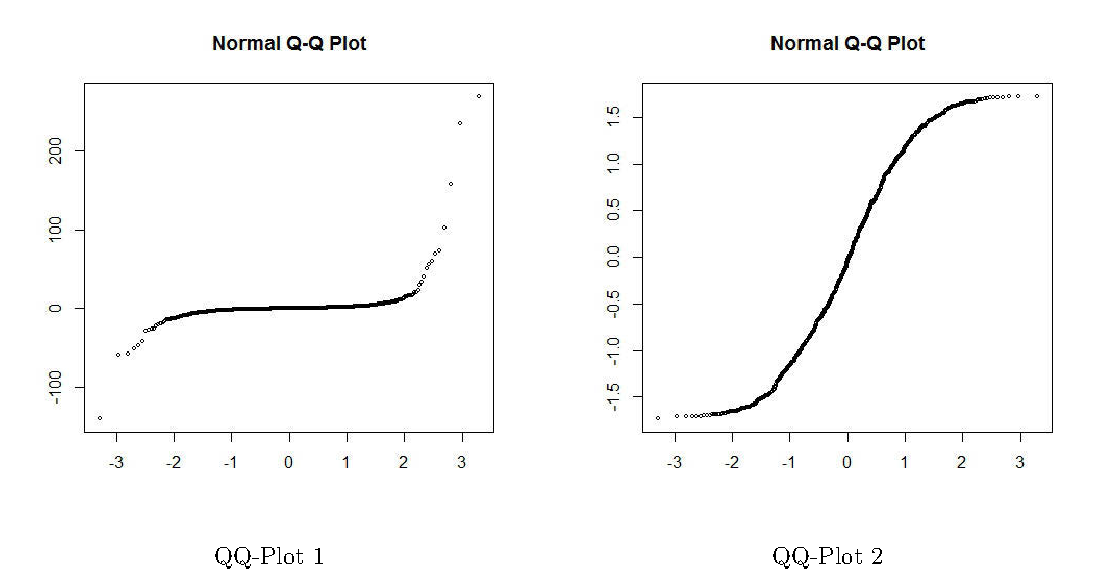
\includegraphics[width=\linewidth]{assignments/assets/ps07-qqplots.pdf}\par
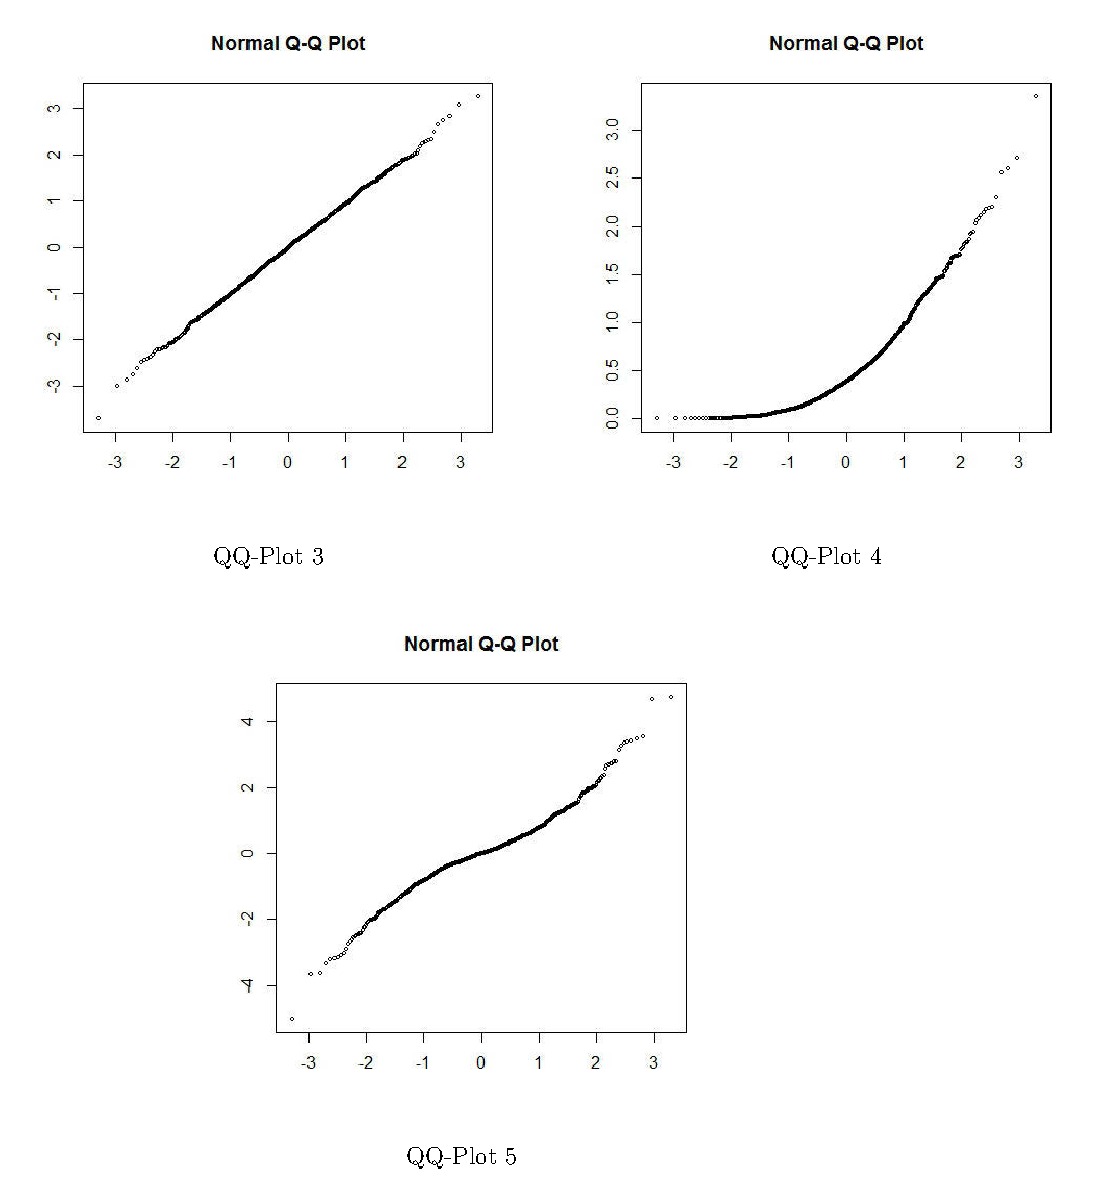
\includegraphics[width=.86\linewidth]{assignments/assets/ps07-qqplots-2.pdf}
\end{center}
\end{exercise}
\begin{solution}
正态 QQ 图将理论正态分位数 $z=\Phi^{-1}(u)$ 与样本经验分位数配对. 总体曲线可用 $F^{-1}(\Phi(z))$ 理解, 样本图围绕该曲线波动. 五图分别是:
\begin{enumerate}[label=图\arabic*:,leftmargin=3em]
\item 柯西分布. 分位数为 $F^{-1}(u)=\tan\{\pi(u-1/2)\}$, 两端发散远快于正态分位数. 图上大部分点挤在零附近, 极端观测达到负百余与正两百余, 是这五个候选中最重的双侧尾.
\item $[-\sqrt3,\sqrt3]$ 上的均匀分布. 总体 QQ 曲线为 $\sqrt3\{2\Phi(z)-1\}$, 近中央斜升, 两端分别趋于 $-\sqrt3$ 与 $\sqrt3$. 图上两端在约 $\pm1.73$ 处变平, 与有界支撑一致.
\item 标准正态分布. 此时 $F^{-1}(\Phi(z))=z$, 因而图形近似斜率1、截距0的直线. 两端有少量抽样波动不改变这一识别.
\item $\operatorname{Exp}(1)$ 分布. 其分位数为 $-\log(1-u)$, 所以总体 QQ 曲线为 $-\log\{1-\Phi(z)\}$. 全部样本非负, 左端贴近0, 右侧向上弯曲并伸出右尾, 图形明显不对称.
\item $\operatorname{Laplace}(\sqrt2)$ 分布. 对 $u<1/2$, 分位数为 $\log(2u)/\sqrt2$; 对 $u\ge1/2$, 为 $-\log\{2(1-u)\}/\sqrt2$. 分布对称且方差为 $2/(\sqrt2)^2=1$, 中央与正态量级接近, 但双侧指数尾比正态尾重. 因而左尾低于直线、右尾高于直线, 尾部偏离比柯西温和, 正是图5.
\end{enumerate}
这些匹配结合了题面限定的五个候选; QQ 图本身不是有限样本下唯一确定分布的证明.
\end{solution}

\begin{exercise}\label{ps07:p02}
原作业第2题. 给定两个独立样本 $X_1,\ldots,X_n$ 与 $Y_1,\ldots,Y_m$, 各样本内部独立同分布, 分布函数分别为 $F,G$. 样本量可不相等. 为简化, 假定两个分布函数连续且递增. 要检验 $H_0:F=G$ 与 $H_1:F\ne G$.
\begin{enumerate}[label=\arabic*.]
\item 给出一个需要判断两个样本是否来自同一分布的实验例子.
\item 令 $U_i=F(X_i)$, $V_j=G(Y_j)$. 求它们的分布.
\item 令 $F_n,G_m$ 为两个样本的经验分布函数.
\begin{enumerate}[label=\alph*)]
\item 定义 $T_{n,m}=\sup_{t\in\R}|F_n(t)-G_m(t)|$. 证明它等于有限个数的最大值.
\item 在 $H_0$ 下证明
\[
T_{n,m}=\sup_{0\le x\le1}\left|\frac1n\sum_{i=1}^n\ind\{U_i\le x\}-\frac1m\sum_{j=1}^m\ind\{V_j\le x\}\right|.
\]
\item 在 $H_0$ 下求 $U_1,\ldots,U_n,V_1,\ldots,V_m$ 的联合分布.
\item 推出 $T_{n,m}$ 为枢轴统计量, 即其原假设分布不依赖未知的总体分布.
\item 给定 $\alpha\in(0,1)$, 令 $q_\alpha$ 为原假设下 $T_{n,m}$ 的 $(1-\alpha)$ 分位数. 如果找不到适合 $n,m$ 的表, 描述一个可在软件(如R)运行的近似分位数算法.
\item 给出非渐近水平 $\alpha$ 的检验.
\end{enumerate}
\end{enumerate}
\end{exercise}
\begin{solution}
\begin{enumerate}[label=\arabic*.]
\item 可随机抽取旧工艺和新工艺生产的电池, 比较其寿命分布. 均值相同并不排除早期失效比例或尾部寿命不同, 所以比较整个分布比只比较均值更符合目标. 两组应相互独立, 各自从固定工艺总体随机抽样.
\item 连续分布函数的概率积分变换给出 $U_i,V_j\sim U[0,1]$. 在严格递增的题设下, 对 $u\in(0,1)$,
$\PP(F(X_i)\le u)=\PP(X_i\le F^{-1}(u))=F(F^{-1}(u))=u$.
同一计算用于 $G$. 变换逐个作用于独立变量, 因此仍保持各样本内部以及两组之间的独立性.
\item
\begin{enumerate}[label=\alph*)]
\item 将合并样本的不同观测值排序为 $w_1<\cdots<w_k$, $k\le n+m$. 两个经验分布函数均在这些点跳跃, 在 $[w_l,w_{l+1})$ 上保持常数; 在第一个点之前均为0, 最后一个点之后均为1. 由右连续性,
\[
T_{n,m}=\max_{1\le l\le k}|F_n(w_l)-G_m(w_l)|.
\]
因此可在有限个观测点精确计算上确界, 不需要连续网格搜索.
\item 在 $H_0$ 下, $F=G$ 且单调变换保持次序, 故 $X_i\le t$ 等价于 $U_i\le F(t)$, $Y_j\le t$ 等价于 $V_j\le F(t)$. 连续递增分布函数的值域含 $(0,1)$, 而端点处两个经验函数的差为0. 因此取 $t\in\R$ 的上确界等于取 $x\in[0,1]$ 的上确界, 得到题中恒等式. 连续但非严格递增的分布函数也可用广义逆证明相同分布结论; 本题使用给定的递增条件即可.
\item 所有 $n+m$ 个变量相互独立且服从 $U[0,1]$. 联合分布为 $[0,1]^{n+m}$ 上的乘积均匀分布.
\item 上问右侧是上述独立均匀向量的确定函数, 故其分布只由整数 $n,m$ 决定, 不涉及 $F$. 这就是原假设下的枢轴性, 而不是宣称备择下也与 $F,G$ 无关.
\item 重复 $B$ 次: 生成 $n+m$ 个独立均匀数, 前 $n$ 个归第一组、后 $m$ 个归第二组; 合并排序并沿排序累积两组计数, 计算最大经验分布差. 将模拟得到的 $B$ 个统计量排序, 取第 $\lceil B(1-\alpha)\rceil$ 个作近似分位数. 下面R代码可直接运行, 不要求输入原始样本:
\begin{verbatim}
ks_stat <- function(x, y) {
  ord <- order(c(x, y))
  lab <- c(rep(1, length(x)), rep(0, length(y)))[ord]
  max(abs(cumsum(lab)/length(x) -
          cumsum(1-lab)/length(y)))
}
ks_quantile <- function(n, m, alpha=.05, B=50000) {
  stopifnot(n>=1, m>=1, alpha>0, alpha<1)
  val <- replicate(B, ks_stat(runif(n), runif(m)))
  sort(val)[ceiling(B*(1-alpha))]
}
set.seed(65007)
ks_quantile(20, 25)
\end{verbatim}
$n=20,m=25$ 只是算法验算的示例, 原题没有指定数值. 对 $\alpha=0.05$, Python 等价算法的50000次模拟得到分位数约0.39. 本项目实际运行了 Python 的等价算法, 没有运行R. 模拟分位数有抽样误差, 不能把有限 $B$ 的估计误说成已知的精确临界值.
\item 定义精确分位数 $q_\alpha=\inf\{q:\PP_0(T_{n,m}\le q)\ge1-\alpha\}$. 当 $T_{n,m}>q_\alpha$ 时拒绝, 则 $\PP_0(T_{n,m}>q_\alpha)\le\alpha$. 此统计量的分布是离散的, 一般不能保证不随机化的检验大小恰为 $\alpha$; “水平 $\alpha$”指至多 $\alpha$. 精确分位数可以枚举合并排序中 $\binom{n+m}{n}$ 种等概率组标签次序求得. 模拟近似临界值本身只近似控制水平.

若只用有限次模拟而仍要求严格有限样本控制, 可生成 $B$ 个独立原假设统计量 $T^{(b)}$, 取
$p_{\rm MC}=\{1+\sum_b\ind(T^{(b)}\ge T_{\rm obs})\}/(B+1)$,
在 $p_{\rm MC}\le\alpha$ 时拒绝. 原假设下观察值与模拟值交换对称; 以大于等于计数使并列保守, 所以秩检验的拒绝概率至多 $\alpha$. 这一规则把模拟随机性也计入检验, 避免将估计分位数当作精确分位数.
\end{enumerate}
\end{enumerate}
\end{solution}

\begin{exercise}\label{ps07:p03}
原作业第3题. 给定独立同分布实随机变量对 $(X_i,Y_i)$, $i=1,\ldots,n$, 其分布连续. 要检验 $H_0:X_1,Y_1\text{ 独立}$ 与 $H_1:X_1,Y_1\text{ 不独立}$. 令 $R_i$ 为 $X_i$ 在 $X_1,\ldots,X_n$ 中的秩, 最小值秩为1, 最大值秩为 $n$; $Q_i$ 为 $Y_i$ 的相应秩.
\begin{enumerate}[label=\arabic*.]
\item 给出需要检验两组观测独立性的实验例子.
\item 不必严格证明, 解释为什么 $R_1,\ldots,R_n$ 不独立.
\item 证明 $R$ 的分布不依赖 $X_i$ 的未知分布, $Q$ 的分布也不依赖 $Y_i$ 的未知分布.
\item 证明在 $H_0$ 下, 两个秩向量 $R,Q$ 相互独立.
\item 推出在 $H_0$ 下, 所有 $2n$ 个秩的联合分布已知且不依赖原样本分布.
\item 定义秩的样本相关系数
\[
T_n=\frac{\sum_i(R_i-\bar R)(Q_i-\bar Q)}{\sqrt{\sum_i(R_i-\bar R)^2\sum_i(Q_i-\bar Q)^2}}.
\]
\begin{enumerate}[label=\alph*)]
\item 证明 $\bar R=\bar Q=(n+1)/2$, $\sum_i(R_i-\bar R)^2=\sum_i(Q_i-\bar Q)^2=n(n^2-1)/12$. 提示: $\sum_{i=1}^ni=n(n+1)/2$, $\sum_{i=1}^ni^2=n(n+1)(2n+1)/6$.
\item 推出 $T_n=12\sum_iR_iQ_i/[n(n^2-1)]-3(n+1)/(n-1)$.
\end{enumerate}
\item 证明在 $H_0$ 下 $T_n$ 与
$S_n=12\sum_iR'_iQ'_i/[n(n^2-1)]-3(n+1)/(n-1)$ 同分布, 其中 $R',Q'$ 来自两组相互独立的独立同分布 $U[0,1]$ 样本.
\item 给定 $\alpha\in(0,1)$, 令 $q_\alpha$ 为 $S_n$ 的 $(1-\alpha)$ 分位数. 描述给定 $n$ 时可在R中近似计算它的算法.
\item 定义 $H_0$ 对 $H_1$ 的非渐近水平 $\alpha$ 检验.
\end{enumerate}
\end{exercise}
\begin{solution}
秩相关要求 $n\ge2$ 且各边际无原子, 于是各组内部几乎处处没有并列值. 这里“连续分布”按无并列所需的边际连续解释; 不额外假定联合密度存在. 若只要求二维分布没有点原子, 却容许边际原子, 原题的无并列秩结论就需另补条件.
\begin{enumerate}[label=\arabic*.]
\item 可以对随机抽取的同一批成年人的每日运动时长与静息心率作成对测量, 检验两者是否独立. 每人的两项观测保持配对, 不同受试者独立抽样.
\item 每个秩只可出现一次. 如果 $R_1=n$, 其余秩都不能再等于 $n$; 知道前 $n-1$ 个秩后, 最后一个秩已被确定. 因此秩之间相互约束, 不是独立变量.
\item 对任意排列 $\pi$, 事件 $X_{\pi(1)}<\cdots<X_{\pi(n)}$ 具有相同概率: 独立同分布使联合分布在任意指标置换下不变. 无并列使这 $n!$ 个事件互斥且覆盖概率1, 所以每个事件概率为 $1/n!$. 每个事件唯一对应一个秩向量, 因而 $R$ 在所有 $\{1,\ldots,n\}$ 的排列上均匀分布. 证明不使用边际分布具体形式. 对 $Q$ 完全相同.
\item 成对样本的联合分布为 $\prod_iP_{XY}$; 在 $H_0$ 下 $P_{XY}=P_X\otimes P_Y$, 所以它重新分组为 $\prod_iP_X\otimes\prod_iP_Y$. 因而整个 $X$ 样本向量与整个 $Y$ 样本向量独立. 可测函数保持独立性, $R=R(X)$ 与 $Q=Q(Y)$ 故独立.
\item 联合秩分布是在 $n!\times n!$ 个排列对上的均匀分布, 每对概率 $1/(n!)^2$. 同一向量内部的秩仍有依赖, 只有两个向量相互独立.
\item
\begin{enumerate}[label=\alph*)]
\item 秩向量只是 $1,\ldots,n$ 的置换, 因而平均为 $(n+1)/2$. 记 $c=(n+1)/2$, 利用题给求和式,
\begin{align*}
\sum_i(R_i-c)^2
&=\frac{n(n+1)(2n+1)}6-2c\frac{n(n+1)}2+nc^2\\
&=n(n+1)\left\{\frac{2n+1}6-\frac{n+1}2+\frac{n+1}4\right\}
=\frac{n(n^2-1)}{12}.
\end{align*}
对 $Q$ 的计算相同, 所以分母是这个确定的正常数.
\item 展开分子, 利用 $\sum_iR_i=\sum_iQ_i=nc$, 得
$\sum_i(R_i-c)(Q_i-c)=\sum_iR_iQ_i-nc^2$.
除以 $n(n^2-1)/12$, 得
\[
T_n=\frac{12}{n(n^2-1)}\sum_iR_iQ_i-
\frac{12nc^2}{n(n^2-1)}
=\frac{12}{n(n^2-1)}\sum_iR_iQ_i-\frac{3(n+1)}{n-1}.
\]
\end{enumerate}
\item 两组独立均匀样本的秩恰有第5问的已知联合分布. 将同一确定函数作用于同分布的 $(R,Q)$ 与 $(R',Q')$, 得 $T_n\stackrel{\mathrm d}=S_n$.
\item 可以逐次产生两组长度 $n$ 的均匀样本, 各自求秩后代入第7问公式; 将 $B$ 个值排序取第 $\lceil B(1-\alpha)\rceil$ 个. 更快的等价算法是在每次模拟生成两个独立均匀随机排列. 由共同指标重排, 还可以固定第一个秩向量为 $1,\ldots,n$, 仅随机生成第二个排列. 下面代码同时给出题面单侧分位数和下一问需要的双侧分位数:
\begin{verbatim}
spearman_quantiles <- function(n, alpha=.05, B=50000) {
  stopifnot(n>=2, alpha>0, alpha<1)
  r <- seq_len(n) - (n+1)/2
  den <- sum(r*r)
  val <- replicate(B, sum(r*(sample.int(n)-(n+1)/2))/den)
  k <- ceiling(B*(1-alpha))
  c(one_sided=sort(val)[k], two_sided=sort(abs(val))[k])
}
set.seed(65007)
spearman_quantiles(10)
\end{verbatim}
本项目运行的是对应 Python 算法, 未运行R. 在 $n=10$, $\alpha=0.05$ 的50000次模拟示例中, 单侧分位数约0.55152, 绝对值分位数约0.63636. 精确分布可在规模允许时枚举 $n!$ 个排列而得. $n=10$ 为验算示例, 不属于原题给定数据.
\item 按原题第8问的单侧 $q_\alpha$, 拒绝规则 $T_n>q_\alpha$ 满足 $\PP_0(T_n>q_\alpha)\le\alpha$, 所以确为非渐近水平 $\alpha$ 的检验. 但原题备择是一般“不独立”, 单侧规则只寻找正秩关联. 例如 $X\sim U[0,1]$, $Y=1-X$, 两者有连续边际且完全相依, 样本秩反序, $T_n=-1$, 该上尾规则无法识别它.

适合正负秩关联的数学版本应令 $c_\alpha$ 为 $|S_n|$ 的 $(1-\alpha)$ 分位数, 在 $|T_n|>c_\alpha$ 时拒绝. 枢轴性给出 $\PP_0(|T_n|>c_\alpha)\le\alpha$. 原题单侧分位数不被暗改成双侧分位数, 二者定义与用途不同. 两种精确规则因离散分布均可能保守; 有限模拟时可沿用上一题的加一 Monte Carlo $p$ 值, 把统计量改成 $|T|$ 以保持双侧水平控制.

即使使用双侧秩相关检验, 也不能声称对所有不独立备择一致. 例如 $X\sim U[-1,1]$, $Y=X^2$, 明显相依, 两边际均连续. 总体秩相关为 $\operatorname{Corr}((X+1)/2,|X|)=0$, 因为 $\E[X|X|]=0$. 此检验针对秩相关偏离零, 不能完全代替一般独立性检验.
\end{enumerate}
\end{solution}

\originalchapter{作业八}\label{chap:ps08}
本章译自 MIT 18.650, Fall 2016 官方 \href{https://ocw.mit.edu/courses/18-650-statistics-for-applications-fall-2016/resources/problem-set-8/}{Problem Set 8}, 截止时间为 2016 年 11 月 4 日星期五中午 12 点. 官方没有附答案, 本章解答为独立推导. 对原题中样本量、可积性及共同边际密度的条件缺口, 在相关解答处明确说明, 不把补充条件伪装成原文.

\begin{exercise}\label{ps08:p01}
原作业第1题. 观察 $n$ 个人的特征 $(X_i,y_i)$, 其中 $y_i\in\R$ 为响应, $X_i\in\R^p$ 为确定性解释变量. 线性回归模型为 $y_i=X_i'\beta+\varepsilon_i$, $i=1,\ldots,n$. 误差向量 $\varepsilon=(\varepsilon_1,\ldots,\varepsilon_n)'$ 为中心正态向量, 已知协方差矩阵 $\Sigma$ 可逆. 本题允许异方差, 不假定误差独立同分布. 令 $X\in\R^{n\times p}$ 的第 $i$ 行为 $X_i'$, $Y=(y_1,\ldots,y_n)'$. 令 $\hat\beta$ 在 $\beta\in\R^p$ 上极小化 $(Y-X\beta)'\Sigma^{-1}(Y-X\beta)$.
\begin{enumerate}[label=\arabic*.]
\item 证明同方差情形 $\Sigma=\sigma^2I_n$, $\sigma^2>0$, 时它退化为最小二乘估计.
\item 证明它也是极大似然估计.
\item 给出使 $\hat\beta$ 唯一定义的 $X$ 的一个充分条件.
\item 此后假定该条件成立, 求 $\hat\beta$ 及其分布.
\item 求偏差和二次风险.
\end{enumerate}
\end{exercise}
\begin{solution}
协方差矩阵半正定且可逆, 因而 $\Sigma$ 正定, $\Sigma^{-1}$ 也正定.
\begin{enumerate}[label=\arabic*.]
\item 此时目标函数为 $\sigma^{-2}\norm{Y-X\beta}^2$. 乘以正常数不改变极小点, 所以极小点集合正是通常的最小二乘估计集合; 若设计不满秩, 两者同样可能不唯一.
\item 条件正态密度为
\[
L(\beta)=(2\pi)^{-n/2}(\det\Sigma)^{-1/2}
\exp\left\{-\frac12(Y-X\beta)'\Sigma^{-1}(Y-X\beta)\right\}.
\]
因 $\Sigma$ 已知, 前面的因子不依赖 $\beta$. 指数函数严格递增, 极大化似然等价于极小化目标函数. 所以其极小点集合也是极大似然估计集合.
\item 充分条件是 $\operatorname{rank}(X)=p$, 它蕴含 $n\ge p$. 对任何非零 $v\in\R^p$, $Xv\ne0$, 从而
$v'X'\Sigma^{-1}Xv=(Xv)'\Sigma^{-1}(Xv)>0$.
因此 $A=X'\Sigma^{-1}X$ 正定, 二次目标严格凸, 极小点唯一. 事实上该条件也是必要的: 若 $Xv=0$ 且 $v\ne0$, 参数 $\beta$ 与 $\beta+tv$ 的目标值对所有 $t$ 相同.
\item 展开目标函数为 $Y'\Sigma^{-1}Y-2\beta'X'\Sigma^{-1}Y+\beta'A\beta$. 梯度为 $-2X'\Sigma^{-1}Y+2A\beta$, 解正规方程得
\[
\hat\beta=A^{-1}X'\Sigma^{-1}Y=\beta+A^{-1}X'\Sigma^{-1}\varepsilon.
\]
正态向量线性变换仍为正态, 其协方差为
\[
A^{-1}X'\Sigma^{-1}\Sigma\Sigma^{-1}XA^{-1}=A^{-1}.
\]
所以 $\hat\beta\sim N_p(\beta,(X'\Sigma^{-1}X)^{-1})$. 亦可把 $\Sigma^{-1/2}Y$ 与 $\Sigma^{-1/2}X$ 作为白化后的响应与设计理解这一估计.
\item 因误差中心化, 偏差 $\E\hat\beta-\beta=0$. 取欧氏平方损失, 二次风险为
\[
\E\norm{\hat\beta-\beta}^2
=\sum_{j=1}^p\E(\hat\beta_j-\beta_j)^2
=\operatorname{tr}\{(X'\Sigma^{-1}X)^{-1}\}.
\]
它不依赖 $\beta$, 但依赖设计与已知误差协方差. 若另采用预测误差损失, 风险对象会不同, 此处明确采用参数的欧氏二次风险.
\end{enumerate}
\end{solution}

\begin{exercise}\label{ps08:p02}
原作业第2题. 设 $(X_i,Y_i)$, $i=1,\ldots,n$, 独立同分布, $X_i\in\R^p$, $p\ge1$, $Y_i\in\R$, 且
$Y_i=X_i'\beta+\varepsilon_i$, $\E\varepsilon_i=0$, $\Cov(X_i,\varepsilon_i)=0$.
在第1--3问假定 $X_1$ 有密度 $g$, $\varepsilon_1$ 给定 $X_1=x$ 的条件密度为 $f_x$.
\begin{enumerate}[label=\arabic*.]
\item 用 $\beta,f_x,g$ 写出似然.
\item 证明 $\beta$ 的极大似然估计不依赖可能未知的 $g$.
\item 假定 $\varepsilon_1$ 与 $X_1$ 独立且 $\varepsilon_1\sim N(0,\sigma^2)$.
\begin{enumerate}[label=\alph*)]
\item 求 $f_x$.
\item 原题声称独立连续 $p$ 维随机向量 $X_1,\ldots,X_n$ 的张成秩几乎处处为 $p$, 并允许不证明使用此结果. 证明 $\beta$ 的极大似然估计等于最小二乘估计并求其表达式.
\item 给定所有 $X_i$ 时, 极大似然估计的条件分布是什么?
\item 极大似然估计有偏吗? 提示: 先求给定 $X_i$ 的条件期望.
\item 求 $\sigma^2$ 的极大似然估计.
\item 构造 $\sigma^2$ 的无偏估计 $\hat\sigma^2$, 求给定 $X_i$ 时 $(n-p)\hat\sigma^2/\sigma^2$ 的条件分布.
\end{enumerate}
\item 令 $p=2$, $X_i=(1,Z_i)'$, 其中标量 $Z_i$ 的方差有限且非零. 原件标量也记作 $X_i$; 这里用 $Z_i$ 区分向量和标量. 不再假定向量设计有密度. 记 $\beta=(a,b)'$, 故 $Y_i=a+bZ_i+\varepsilon_i$.
\begin{enumerate}[label=\alph*)]
\item 写出最小二乘估计 $(\hat a,\hat b)$.
\item 证明它一致.
\item 假定 $Z_1$ 与 $\varepsilon_1$ 独立, 记 $\sigma^2=\Var(\varepsilon_1)$. 证明 $(\hat a,\hat b)$ 渐近正态, 用 $\sigma^2$ 与 $Z_1$ 的矩写出渐近协方差矩阵.
\item 当 $Z_1$ 的矩与 $\sigma^2$ 均未知时, 构造 $H_0:b>0$ 的渐近水平至多 $\alpha\in(0,1)$ 的检验.
\end{enumerate}
\end{enumerate}
\end{exercise}
\begin{solution}
前两问把误差条件密度族 $f_x$ 视作给定、不随 $\beta$ 变化的模型部分; 未知边际密度 $g$ 是与 $\beta$ 分开的干扰参数. 若连 $f_x$ 也任意未知, 只消去 $g$ 并不足以指定可计算的极大似然估计.
\begin{enumerate}[label=\arabic*.]
\item 变换 $\varepsilon_i=Y_i-X_i'\beta$ 对 $Y_i$ 的雅可比为1. 单对观测的联合密度为 $g(x_i)f_{x_i}(y_i-x_i'\beta)$, 因而
\[
L(\beta)=\prod_{i=1}^ng(x_i)\prod_{i=1}^nf_{x_i}(y_i-x_i'\beta).
\]
\item 对固定观测, 第一项是不依赖 $\beta$ 的乘数, 所以只须极大化第二项, 即响应给定设计的条件似然. 如果极大点存在, 其集合不依赖 $g$. 未知 $g$ 的存在不改变这个关于 $\beta$ 的优化问题.
\item
\begin{enumerate}[label=\alph*)]
\item 由独立性, 对所有需要的 $x$, $f_x(e)=(2\pi\sigma^2)^{-1/2}\exp(-e^2/(2\sigma^2))$, 不依赖 $x$. 条件密度在零概率的 $x$ 集合上的版本可任意选取, 不影响似然的几乎处处结论.
\item 令 $X$ 为行向量 $X_i'$ 组成的 $n\times p$ 矩阵, $Y=(Y_i)'$. 原题的满秩断言必须补 $n\ge p$, 因为矩阵秩至多 $n$; $n<p$ 时它是错误的. 由于每个 $X_i$ 在 $\R^p$ 有密度, $n\ge p$ 时前 $p$ 行行列式为零的集合是一个非零多项式的零集, 其 Lebesgue 测度为零, 故 $X$ 几乎处处满列秩. 给定这样的设计, 正态对数似然中关于 $\beta$ 的项为 $-\norm{Y-X\beta}^2/(2\sigma^2)$, 所以
\[
\hat\beta=(X'X)^{-1}X'Y=\beta+(X'X)^{-1}X'\varepsilon.
\]
正规方程及 $X'X$ 的正定性保证唯一. 当 $n<p$ 时, 最小二乘拟合仍可定义, 但参数估计一般不唯一.
\item 样本对独立同分布且每个误差独立于本对设计, 故给定整个 $X$ 后 $\varepsilon\sim N_n(0,\sigma^2I_n)$. 因而
\[
\hat\beta\mid X\sim N_p\{\beta,\sigma^2(X'X)^{-1}\}.
\]
无条件分布是随设计变化的正态混合, 通常不能说仍为一个固定协方差的正态分布.
\item 条件期望为 $\E(\hat\beta\mid X)=\beta$. 若各分量绝对可积, 再用全期望公式得 $\E\hat\beta=\beta$, 即无偏. 原题条件本身却不保证这种可积性: 取 $p=n=1$, $X_1\sim U[-1,1]$, 独立误差 $N(0,\sigma^2)$, 则 $\hat\beta=\beta+\varepsilon_1/X_1$, 且
$\E|\varepsilon_1/X_1|=\E|\varepsilon_1|\,\E|1/X_1|=\infty$.
其正负部分均有无穷期望, 无条件期望未定义, 因而不能无条件声称无偏. 准确结论是条件无偏, 以及可积时无条件无偏. 例如 $\E\operatorname{tr}(X'X)^{-1}<\infty$ 足以由二阶矩保证可积.
\item 给定 $\beta$, 关于 $v=\sigma^2$ 的对数似然为 $-n\log v/2-\operatorname{RSS}(\beta)/(2v)$, 其中 $\operatorname{RSS}(\beta)=\norm{Y-X\beta}^2$. 先对 $\beta$ 极大化后, 当最小残差平方和 $\operatorname{RSS}>0$ 时, 求导得
$\hat\sigma_{\rm ML}^2=\operatorname{RSS}/n$, 因为导数 $(-nv+\operatorname{RSS})/(2v^2)$ 在该点前正后负. 给定满秩设计且 $n>p$, 非退化正态误差使 $\operatorname{RSS}>0$ 几乎处处. 当 $n=p$ 且 $X$ 可逆时, 可以完全插值, $\operatorname{RSS}=0$; 在参数域 $v>0$ 中似然随 $v\downarrow0$ 无界, 不存在有限方差极大似然估计. 所以公式中的零只能是边界形式, 不能称为参数域内的极大点.
\item 本问须 $n>p$. 令 $P=X(X'X)^{-1}X'$, 它是秩 $p$ 的正交投影, 残差为 $(I-P)\varepsilon$. 给定 $X$, 用正交基对角化 $I-P$, 它有 $n-p$ 个特征值1及 $p$ 个特征值0. 旋转后的标准化误差仍由独立标准正态坐标组成, 故
\[
\operatorname{RSS}/\sigma^2\mid X\sim\chi^2_{n-p}.
\]
取 $\hat\sigma^2=\operatorname{RSS}/(n-p)$, 得条件期望 $\sigma^2$, 所以也无条件无偏, 且所问比值条件服从 $\chi^2_{n-p}$. 此处条件二次型的期望固定且有限, 不存在上一问的逆矩阵可积性障碍.
\end{enumerate}
\item 以下记 $\mu=\E Z_1$, $v=\Var Z_1>0$, $m_2=\E Z_1^2=\mu^2+v$.
\begin{enumerate}[label=\alph*)]
\item 令 $S_{ZZ}=\sum_i(Z_i-\bar Z)^2$. 当 $S_{ZZ}>0$ 时, 对截距与斜率求偏导得到 $\hat a=\bar Y-\hat b\bar Z$ 以及
\[
\hat b=\frac{\sum_i(Z_i-\bar Z)(Y_i-\bar Y)}{S_{ZZ}}.
\]
若 $S_{ZZ}=0$, 最小二乘斜率不唯一, 可规定 $\hat b=0,\hat a=\bar Y$ 为其中一个解. 非退化总体并不排除有限样本所有设计值相等, 因此不能省略此事件.
\item 将回归模型代入, 得
\[
\hat b-b=
\frac{n^{-1}\sum_i Z_i\varepsilon_i-\bar Z\bar\varepsilon}
 {n^{-1}\sum_iZ_i^2-\bar Z^2},\qquad
\hat a-a=\bar\varepsilon-(\hat b-b)\bar Z.
\]
由 $\E\varepsilon_1=0$, $\Cov(Z_1,\varepsilon_1)=0$, 有 $\E(Z_1\varepsilon_1)=0$. 在题中协方差存在的可积性条件下, 大数定律使分子趋于0, 分母趋于 $m_2-\mu^2=v>0$, $\bar\varepsilon\pto0$, $\bar Z\pto\mu$. 因而 $\hat b\pto b$, $\hat a\pto a$. 分母趋于正常数还表明 $\PP(S_{ZZ}=0)\to0$, 上问在该事件的定义不影响一致性.
\item 本问采用 $\sigma^2<\infty$. 设 $W_i=(1,Z_i)'$, $M=\E W_iW_i'=\begin{pmatrix}1&\mu\\\mu&m_2\end{pmatrix}$. 独立性与误差中心化给出 $\E(W_i\varepsilon_i)=0$ 和
$\E(\varepsilon_i^2W_iW_i')=\sigma^2M$.
因此向量 $W_i\varepsilon_i$ 有有限协方差, 多元中心极限定理给出 $n^{-1/2}\sum_iW_i\varepsilon_i\dto N_2(0,\sigma^2M)$. 另一方面 $M_n=n^{-1}\sum_iW_iW_i'\pto M$, $\det M=v>0$. 正规方程写成
\[
\sqrt n\left\{\begin{pmatrix}\hat a\\\hat b\end{pmatrix}
-\begin{pmatrix}a\\b\end{pmatrix}\right\}
=M_n^{-1}\frac1{\sqrt n}\sum_iW_i\varepsilon_i
\dto N_2(0,\sigma^2M^{-1}).
\]
求二阶逆矩阵即得渐近协方差
\[
\frac{\sigma^2}{v}\begin{pmatrix}m_2&-\mu\\-\mu&1\end{pmatrix}.
\]
这里指 $\sqrt n$ 缩放后的极限协方差; 未缩放估计的近似协方差还要除以 $n$.
\item 在(c)的独立同方差、$0<\sigma^2<\infty$ 条件下, 令 $\hat v=n^{-1}S_{ZZ}$, $\hat e_i=Y_i-\hat a-\hat bZ_i$, $\tilde\sigma^2=n^{-1}\sum_i\hat e_i^2$. 为说明一致性, 将 $\hat e_i=\varepsilon_i-W_i'(\hat\beta-\beta)$ 平方平均; 第一项 $n^{-1}\sum_i\varepsilon_i^2\pto\sigma^2$, 交叉项因 $n^{-1}\sum_iW_i\varepsilon_i\pto0$ 且 $\hat\beta-\beta\pto0$ 而趋零, 二次项 $(\hat\beta-\beta)'M_n(\hat\beta-\beta)\pto0$. 因而 $\tilde\sigma^2\pto\sigma^2$, $\hat v\pto v$.

取 $Z_n=\sqrt{n\hat v}\,\hat b/\tilde\sigma$, 当 $Z_n<z_\alpha$ 时拒绝 $H_0:b>0$, 备择为 $b\le0$. 在边界 $b=0$ 下, (c)及Slutsky定理给出 $Z_n\dto N(0,1)$; 对固定 $b>0$, $Z_n\pto+\infty$, 拒绝概率趋于0, 所以对每个原假设参数的渐近错误率至多 $\alpha$.

在 $S_{ZZ}>0$ 且 $\tilde\sigma>0$ 的事件上, 对固定的设计和误差样本, 将响应的真实斜率由0增至 $b>0$ 只把 $\hat b$ 增加 $b$, 残差、$\hat v$ 与 $\tilde\sigma$ 均不变. 因而在固定的设计与误差分布下, $b>0$ 上的拒绝概率上确界为边界概率, 渐近为 $\alpha$. 若要对所有只有有限二阶矩的未知总体同时给出统一的收敛速率, 原题没有提供足够条件, 此处不作该更强承诺. 分母为零的事件规定不拒绝, 其概率在上述非退化条件下趋零. 若 $\sigma^2=0$, 则误差几乎处处为零, 无需正态近似: 可在 $S_{ZZ}>0$ 时由精确的 $\hat b\le0$ 拒绝, 在 $S_{ZZ}=0$ 时不拒绝. 在 $H_0$ 下这个规则的错误率为0.
\end{enumerate}
\end{enumerate}
\end{solution}

\begin{exercise}\label{ps08:p03}
原作业第3题. 设 $(X_i,Y_i)$, $i=1,\ldots,n$, 为相互独立的随机对, $Y_i\in\{0,1\}$, $X_i\in\R^p$, 且
\[
\log\frac{\PP(Y_i=1\mid X_i)}{\PP(Y_i=0\mid X_i)}=X_i'\beta,
\qquad\beta\in\R^p.
\]
原题为简化假定 $X_1$ 有未知密度 $f$.
\begin{enumerate}[label=\arabic*.]
\item 求 $\PP(Y_i=1\mid X_i)$.
\item 用 $\beta$ 与 $f$ 写出模型似然.
\item 证明 $\beta$ 的极大似然估计不依赖未知密度 $f$. 原题注: 该估计通常没有闭式, 但有算法可近似计算.
\end{enumerate}
\end{exercise}
\begin{solution}
\begin{enumerate}[label=\arabic*.]
\item 记 $\eta_i=X_i'\beta$, $\pi_i=\PP(Y_i=1\mid X_i)$. 由 $\pi_i/(1-\pi_i)=e^{\eta_i}$, 解得
$\pi_i=e^{\eta_i}/(1+e^{\eta_i})=1/(1+e^{-\eta_i})$,
$1-\pi_i=1/(1+e^{\eta_i})$.
\item 原题只写各对独立, 不写同分布, 又只明确 $X_1$ 有密度 $f$. 要用同一个 $f$ 写所有观测的联合似然, 需补充所有 $X_i$ 有共同边际密度 $f$. 在此数学版本下, 对 $x$ 的 Lebesgue 测度与 $y$ 的计数测度, 联合似然为
\begin{align*}
L(\beta,f)&=\prod_{i=1}^nf(x_i)\pi_i^{y_i}(1-\pi_i)^{1-y_i}\\
&=\left\{\prod_{i=1}^nf(x_i)\right\}
\exp\left\{\sum_{i=1}^n[y_ix_i'\beta-\log(1+e^{x_i'\beta})]\right\}.
\end{align*}
若各 $X_i$ 有不同密度 $f_i$, 则第一因子改为 $\prod_if_i(x_i)$, 条件似然部分完全相同. 只假定 $X_1$ 有密度时, 仍可使用给定所有设计的条件似然, 但不能无根据给其他 $X_i$ 指定 $f$.
\item 边际密度因子不依赖 $\beta$, 因而若有限极大点存在, 它是条件对数似然
\[
\ell(\beta)=\sum_i\{y_ix_i'\beta-\log(1+e^{x_i'\beta})\}
\]
的极大点, 与 $f$ 无关. 其梯度为 $\sum_ix_i(y_i-\pi_i)=X'(Y-\pi)$, Hessian为
$-\sum_i\pi_i(1-\pi_i)x_ix_i'=-X'DX$,
其中 $D$ 的对角元为 $\pi_i(1-\pi_i)>0$. 满列秩设计时Hessian负定, 有限极大点若存在则唯一, 可通过 Newton 迭代
$\beta_{\rm new}=\beta+(X'DX)^{-1}X'(Y-\pi)$
寻找, 必要时缩短步长以增加似然. 这解释原题所说的算法近似, 而不声称存在闭式解.

原题条件也不保证有限极大点存在. 例如 $p=1$, 所有观测 $x_i>0,y_i=1$, 则 $\ell(\beta)=\sum_i\log\{1/(1+e^{-x_i\beta})\}$ 随 $\beta$ 严格增加, 当 $\beta\to+\infty$ 趋于0, 任意有限 $\beta$ 都达不到上确界. 即使 $X_i$ 有共同连续密度且支持在 $[1,2]$, 在有限真实参数下全部 $Y_i=1$ 仍有正概率. 因而准确结论是优化目标不依赖 $f$, 且当MLE存在时MLE不依赖 $f$; 不能由此自动推出存在性.
\end{enumerate}
\end{solution}

\originalchapter{作业九}\label{chap:ps09}
本章对应 MIT 18.650 Fall 2016 的 \href{https://ocw.mit.edu/courses/18-650-statistics-for-applications-fall-2016/resources/problem-set-9/}{Problem Set 9}. 原截止时间为 2016 年 11 月 18 日星期五中午 12 时. 题面译自官方原件, 解答为独立推导.

\begin{exercise}\label{ps09:p01}
原作业第1题. 固定设计的非参数回归（60 分）.
在 $[0,1]$ 上取固定的等距设计 $x_i=i/n$, $i=0,\ldots,n$. 观测为 $Y_i=f(x_i)+\varepsilon_i$, 其中 $f$ 是 $[0,1]$ 上未知函数, $\varepsilon_0,\ldots,\varepsilon_n\iid N(0,\sigma^2)$, $\sigma^2>0$. 假设 $f$ 可微且对所有 $x\in[0,1]$ 有 $|f'(x)|\le L$, 其中 $L>0$. 目标是估计 $f$. 取整数 $1\le k\le n$, 定义 $I_i=\{j\in\{0,\ldots,n\}:|j-i|\le k\}$.
\begin{enumerate}[label=\arabic*.]
\item 对每个 $i\in\{0,\ldots,n\}$ 计算 $|I_i|$, 并证明 $k+1\le |I_i|\le2k+1$.
\item 用 $\widehat f_i=|I_i|^{-1}\sum_{j\in I_i}Y_j$ 估计 $f(x_i)$.
\begin{enumerate}[label=\alph*)]
\item 计算 $\widehat f_i$ 的方差, 并证明 $\Var(\widehat f_i)\le\sigma^2/k$.
\item 计算 $\E\widehat f_i$, 并证明其偏差 $b_i$ 满足 $|b_i|\le |I_i|^{-1}\sum_{j\in I_i}|f(x_j)-f(x_i)|$.
\item 利用 $f$ 的条件证明 $b_i^2\le L^2k^2/n^2$.
\item 证明二次风险满足 $\E[(\widehat f_i-f(x_i))^2]\le L^2k^2/n^2+\sigma^2/k$.
\item 怎样选择 $k$ 能使上述风险上界最小?
\item 对该选择, 二次风险趋于零的收敛速率是什么?
\item 证明即使不知道 $L$ 与 $\sigma^2$, 仍可选择不依赖这两个量的 $k$, 使风险的阶仍为 $n^{-2/3}$.
\end{enumerate}
\item （选做）令 $\widehat f$ 是满足 $\widehat f(x_i)=\widehat f_i$ 的分段线性函数, 此处仍取任意整数 $1\le k\le n$. 定义积分二次风险
\[
R(\widehat f,f)=\E\left[\int_0^1(\widehat f(x)-f(x))^2\dd x\right].
\]
证明 $R(\widehat f,f)\le c_1k^2/n^2+c_2/k$, 其中正常数 $c_1,c_2$ 只依赖 $L,\sigma^2$. 推出存在一个 $k$ 的选择使风险以 $n^{-2/3}$ 的速率趋于零.
\end{enumerate}
\end{exercise}
\begin{solution}
局部平均减少噪声, 但也混入相邻位置的函数值. 计算中把这两种误差分别写成方差与偏差, 才能看出窗口宽度 $k$ 的取舍.
\begin{enumerate}[label=\arabic*.]
\item 可用的最小、最大下标分别是 $\max(0,i-k)$ 和 $\min(n,i+k)$, 故
\[
m_i:=|I_i|=\min(n,i+k)-\max(0,i-k)+1
=1+\min(k,i)+\min(k,n-i).
\]
两个最小值均不超过 $k$, 因而 $m_i\le2k+1$. 下界不能只假设至少一侧有 $k$ 个点, 因为 $k$ 很大时两侧都可能不足. 若其中一侧不少于 $k$, 两项之和至少是 $k$; 若两侧均小于 $k$, 两项之和是 $i+(n-i)=n\ge k$. 所以总有 $m_i\ge k+1$.
\item
\begin{enumerate}[label=\alph*)]
\item $f(x_j)$ 是常数, 噪声独立, 所以 $\Var(\widehat f_i)=m_i^{-2}\sum_{j\in I_i}\sigma^2=\sigma^2/m_i\le\sigma^2/(k+1)\le\sigma^2/k$.
\item 零均值噪声给出 $\E\widehat f_i=m_i^{-1}\sum_{j\in I_i}f(x_j)$. 因此
\[
b_i=\E\widehat f_i-f(x_i)
=\frac1{m_i}\sum_{j\in I_i}\bigl(f(x_j)-f(x_i)\bigr),
\]
取绝对值并用三角不等式即得所需上界.
\item 由中值定理, $|f(x_j)-f(x_i)|\le L|x_j-x_i|=L|j-i|/n\le Lk/n$. 代入上问的平均后得 $|b_i|\le Lk/n$, 平方即为结论.
\item 写成 $\widehat f_i-f(x_i)=(\widehat f_i-\E\widehat f_i)+b_i$. 第一项期望为零, 展开平方后的交叉项消失, 故风险等于 $\Var(\widehat f_i)+b_i^2$, 从而得到题给上界.
\item 先把 $k$ 暂看成正实数, 记 $B(t)=L^2t^2/n^2+\sigma^2/t$. 则
\[
B'(t)=2L^2t/n^2-\sigma^2/t^2,\qquad
B''(t)=2L^2/n^2+2\sigma^2/t^3>0.
\]
唯一无约束最小点为 $t_*=(\sigma^2n^2/(2L^2))^{1/3}$. 在区间 $[1,n]$ 上先截断为 $\widetilde t=\min(n,\max(1,t_*))$, 然后比较 $\lfloor\widetilde t\rfloor$ 和 $\lceil\widetilde t\rceil$ 中属于 $\{1,\ldots,n\}$ 的值, 取 $B$ 较小者. 严格凸性及最小点两侧的单调性保证这就是整数最优选择; 不能不加说明地把非整数 $t_*$ 当作窗口大小.
\item 固定 $L,\sigma^2>0$, 当 $n$ 足够大时 $1<t_*<n$. 此时 $B(t_*)=3\cdot2^{-2/3}L^{2/3}(\sigma^2)^{2/3}n^{-2/3}$. 取整带来的相对改变量趋于零, 因此风险为 $O(n^{-2/3})$.
\item 可取 $k=\lceil n^{2/3}\rceil$, 对整数 $n\ge1$ 有 $1\le k\le n$, 且 $n^{2/3}\le k\le2n^{2/3}$. 因此
\[
\E[(\widehat f_i-f(x_i))^2]
\le(4L^2+\sigma^2)n^{-2/3}.
\]
常数可依赖未知的 $L,\sigma^2$, 但实施窗口选择不需知道它们.
\end{enumerate}
\item 对 $x\in[x_i,x_{i+1}]$, 记 $t=n(x-x_i)\in[0,1]$. 则 $\widehat f(x)=(1-t)\widehat f_i+t\widehat f_{i+1}$. 先对真实函数做同样插值 $f_\ell(x)=(1-t)f(x_i)+tf(x_{i+1})$. Lipschitz 条件给出
\[
|f_\ell(x)-f(x)|\le (1-t)Lt/n+tL(1-t)/n
=2Lt(1-t)/n\le L/(2n).
\]
所以插值估计的偏差绝对值不超过 $(1-t)|b_i|+t|b_{i+1}|+L/(2n)\le L(k+1/2)/n\le3Lk/(2n)$. 相邻估计共享噪声, 不能假设它们独立. 由 Cauchy--Schwarz 不等式, 两者协方差的绝对值不超过其标准差之积, 因而
\[
\Var(\widehat f(x))\le
\left((1-t)\sqrt{\Var(\widehat f_i)}+t\sqrt{\Var(\widehat f_{i+1})}\right)^2
\le\sigma^2/k.
\]
于是每个 $x$ 的均方误差至多 $9L^2k^2/(4n^2)+\sigma^2/k$. 非负被积函数可由 Tonelli 定理交换积分和期望, 并且积分区间长度为 $1$, 故可取 $c_1=9L^2/4$, $c_2=\sigma^2$. 再取 $k=\lceil n^{2/3}\rceil$ 即得 $R(\widehat f,f)=O(n^{-2/3})$.
\end{enumerate}
\end{solution}
\begin{remark}
上面先证明了 $O(n^{-2/3})$ 上界. 对已选的 $k\asymp n^{2/3}$, 还可由 $\Var(\widehat f_i)=\sigma^2/|I_i|\ge\sigma^2/(2k+1)$ 得到匹配下界, 因此这个窗口选择下的节点风险对每个 $f$ 都是 $\Theta(n^{-2/3})$. 即使 $f$ 是常函数、偏差为零, 此方差下界仍成立. 这不等于证明该函数类上的 minimax 最优速率: 后者还需要对所有可能估计器的最坏情形风险作统一下界.
\end{remark}

\begin{exercise}\label{ps09:p02}
原作业第2题. 密度的非参数估计（40 分）.
设 $X_1,\ldots,X_n$ 独立同分布于 $[0,1]$, 未知密度为 $f$. 本题始终假设 $f$ 可微, 且 $|f(x)|\le L$, $|f'(x)|\le L$ 对所有 $x\in[0,1]$ 成立, $L>0$ 为固定常数. 对 $h>0$ 定义
\[
\widehat f(x)=\frac1{2nh}\sum_{i=1}^n\ind_{\{|X_i-x|\le h\}},\qquad x\in[0,1].
\]
以下取 $x\in(h,1-h)$.
\begin{enumerate}[label=\arabic*.]
\item 每个 $\ind_{\{|X_i-x|\le h\}}$ 的分布是什么?
\item 记 $\widehat f(x)$ 的偏差为 $b(x)$、方差为 $\sigma^2(x)$. 回顾二次风险与二者的关系.
\item 证明 $b(x)=[F(x+h)-F(x-h)-2hf(x)]/(2h)$, 其中 $F$ 是 $X_1$ 的分布函数.
\item 利用 Taylor 公式证明 $|b(x)|\le Lh/2$.
\item 证明 $\sigma^2(x)\le L/(2nh)$.
\item 用前面各问给出二次风险上界.
\item 证明即使不知道 $L$, 仍可选择窗口宽度 $h$, 使二次风险不超过 $Cn^{-2/3}$, 其中 $C>0$ 只依赖 $L$.
\end{enumerate}
\end{exercise}
\begin{solution}
\begin{enumerate}[label=\arabic*.]
\item 指示变量只取 $0,1$, 所以服从 $\operatorname{Ber}(p_h(x))$, 其中 $p_h(x)=\PP(x-h\le X_i\le x+h)=F(x+h)-F(x-h)=\int_{x-h}^{x+h}f(u)\dd u$. 密度分布在端点没有原子, 因而闭区间或开区间不影响概率. 不同 $i$ 的指示变量仍独立同分布.
\item 展开中心化误差的平方, 得 $\E[(\widehat f(x)-f(x))^2]=b(x)^2+\sigma^2(x)$.
\item $\E\widehat f(x)=p_h(x)/(2h)$, 减去 $f(x)$ 即得题给等式.
\item 也可把该等式写成 $b(x)=(2h)^{-1}\int_{-h}^h[f(x+u)-f(x)]\dd u$. 对每个 $u$ 用一阶 Taylor 的中值余项, 或等价的中值定理, 有 $|f(x+u)-f(x)|\le L|u|$. 不需要假设二阶导数存在. 因此
\[
|b(x)|\le\frac{L}{2h}\int_{-h}^h|u|\dd u
=\frac{Lh}{2}.
\]
\item Bernoulli 方差为 $p_h(x)(1-p_h(x))$. 利用独立性,
\[
\sigma^2(x)=\frac{p_h(x)(1-p_h(x))}{4nh^2}
\le\frac{p_h(x)}{4nh^2}.
\]
又因 $0\le f\le L$, 有 $p_h(x)\le2hL$, 所以 $\sigma^2(x)\le L/(2nh)$.
\item 两个上界相加给出 $\E[(\widehat f(x)-f(x))^2]\le L^2h^2/4+L/(2nh)$.
\item 取 $h=n^{-1/3}$, 对所有满足 $x\in(h,1-h)$ 的点,
\[
\E[(\widehat f(x)-f(x))^2]\le
\left(\frac{L^2}{4}+\frac L2\right)n^{-2/3}.
\]
若先固定 $x\in(0,1)$, 则当 $n$ 足够大时 $n^{-1/3}<\min(x,1-x)$, 上述内部点条件自然成立. 因而这里的速率是内部点的渐近结论, 常数 $C=L^2/4+L/2$ 不依赖 $x$ 或未知密度的其他特征.
\end{enumerate}
\end{solution}
\begin{remark}
内部点条件不可删除. 例如均匀密度 $f\equiv1$ 在 $x=0$ 时给出 $\E\widehat f(0)=1/2$（$h\le1$）, 偏差恒为 $-1/2$. 原式未作边界修正, 因此不能由本题推出全区间的一致点态风险速率.
\end{remark}

\originalchapter{作业十}\label{chap:ps10}
本章对应 MIT 18.650 Fall 2016 的 \href{https://ocw.mit.edu/courses/18-650-statistics-for-applications-fall-2016/resources/problem-set-10/}{Problem Set 10}. 原截止时间为 2016 年 12 月 2 日星期五中午 12 时. 题面译自官方原件, 解答为独立推导.

\begin{exercise}\label{ps10:p01}
原作业第1题. 贝叶斯估计.
设 $X_1,\ldots,X_n\iid N(0,\theta)$, 其中 $\theta>0$ 未知.
\begin{enumerate}[label=\arabic*.]
\item 计算 $\theta$ 的极大似然估计.
\item 证明该估计渐近正态, 并求其渐近方差.
\item 在贝叶斯方法中:
\begin{enumerate}[label=\alph*)]
\item 计算 Jeffreys 先验. 它是正常先验吗?
\item 用 Bayes 公式计算后验分布. 它是否有良好定义?
\item 计算对应 Jeffreys 先验的贝叶斯估计.
\end{enumerate}
\end{enumerate}
原题提示: 参数 $\alpha>1$, $\beta>0$ 的逆 Gamma 分布具有密度 $\beta^\alpha e^{-\beta/x}/[\Gamma(\alpha)x^{\alpha+1}]$, $x>0$, 其期望为 $\beta/(\alpha-1)$.
\end{exercise}
\begin{solution}
记 $S=\sum_{i=1}^nX_i^2$. 这里 $\theta$ 是方差参数, 不是标准差.
\begin{enumerate}[label=\arabic*.]
\item 对数似然为 $\ell_n(\theta)=-\frac n2\log(2\pi)-\frac n2\log\theta-\frac S{2\theta}$. 因而 $\ell_n'(\theta)=(S-n\theta)/(2\theta^2)$. 当 $S>0$ 时导数在 $S/n$ 左侧为正、右侧为负, 唯一极大值是 $\widehat\theta=S/n$. 若所有观测恰为零, 则似然随 $\theta\downarrow0$ 无界, 在开参数空间上没有极大值. 在真实的 $\theta>0$ 下该事件概率为零, 所以 $S/n$ 是几乎处处定义的 MLE.
\item 对 $X\sim N(0,\theta)$, 写 $X=\sqrt\theta Z$, $Z\sim N(0,1)$. 标准正态积分的分部积分给出 $\E Z^2=1$, $\E Z^4=3$（递推式为 $\E Z^{2r}=(2r-1)\E Z^{2r-2}$）, 所以 $\E X^2=\theta$, $\Var(X^2)=3\theta^2-\theta^2=2\theta^2$. 对独立同分布的 $X_i^2$ 应用中心极限定理,
\[
\sqrt n(\widehat\theta-\theta)\dto N(0,2\theta^2).
\]
故渐近方差按 $\sqrt n$ 归一化的约定为 $2\theta^2$; 原估计量的方差恰为 $2\theta^2/n$.
\item
\begin{enumerate}[label=\alph*)]
\item 单次观测的得分为 $s_\theta(X)=(X^2-\theta)/(2\theta^2)$. 其平方期望是 $I(\theta)=2\theta^2/(4\theta^4)=1/(2\theta^2)$. Jeffreys 先验密度正比于 $\sqrt{I(\theta)}$, 因而 $\pi(\theta)\propto1/\theta$, $\theta>0$. 其在 $(0,\infty)$ 上的积分发散, 无法归一化, 所以是不正常先验. 使用全样本信息只会多一个与 $\theta$ 无关的因子 $\sqrt n$, 不改变先验.
\item 似然乘先验给出后验核 $\theta^{-n/2-1}\exp[-S/(2\theta)]$. 对 $S>0$, 用代换 $u=S/(2\theta)$ 可算得
\[
\int_0^\infty\theta^{-n/2-1}e^{-S/(2\theta)}\dd\theta
=\left(\frac S2\right)^{-n/2}\Gamma(n/2).
\]
所以后验为 $\operatorname{InvGamma}(n/2,S/2)$, 密度是
\[
\pi(\theta\mid X)=\frac{(S/2)^{n/2}}{\Gamma(n/2)}
\theta^{-n/2-1}e^{-S/(2\theta)},\qquad\theta>0.
\]
任何 $n\ge1$ 时, $n/2>0$, 该密度都可归一化. 不正常先验并不阻止这里的后验成为概率分布. 但若 $S=0$, 后验核在零附近不可积, 所以该异常样本下后验未定义.
\item 按平方损失理解贝叶斯估计时, 后验均值是
\[
\widehat\theta_B=\E[\theta\mid X]
=\frac{S/2}{n/2-1}=\frac S{n-2},\qquad n>2.
\]
可直接对后验密度乘 $\theta$ 后积分核验: 同一代换给出 $\E[\theta\mid X]=(S/2)\Gamma(n/2-1)/\Gamma(n/2)$, 并利用 $\Gamma(z+1)=z\Gamma(z)$. 若 $n\le2$, 尾部的均值积分与 $\int^\infty\theta^{-n/2}\dd\theta$ 同阶而发散, 后验均值不存在有限值.

还须区分“后验均值存在”与“后验平方风险有限”: $n>4$ 时二阶矩有限, 此时对任意决策 $a$ 有 $\E[(\theta-a)^2\mid X]=\Var(\theta\mid X)+(a-\E[\theta\mid X])^2$, 唯一最小值在上述均值. 对 $n=3,4$, 均值虽然有限, 但所有有限 $a$ 的后验平方损失期望均为无穷大, 因而若严格用有限后验平方风险的最优决策定义, 还需 $n>4$; 通常作业所指的后验均值仍按 $n>2$ 的公式报告.
\end{enumerate}
\end{enumerate}
\end{solution}
\begin{remark}
原题未对第 3(c) 问给出样本量限制, 也未显式指定损失函数. 上述解答明确采用后验均值的通常平方损失约定, 补出均值存在所需的 $n>2$. 提示中的逆 Gamma 密度其实对所有 $\alpha>0$ 都能定义; $\alpha>1$ 是均值有限的条件.
\end{remark}

\begin{exercise}\label{ps10:p02}
原作业第2题. 贝叶斯估计与线性回归.
设 $X_1,\ldots,X_n$ 为 $\R^p$ 中的确定向量, $X$ 为第 $i$ 行等于 $X_i'$ 的 $n\times p$ 矩阵. 给定某个 $p$ 维随机向量 $\beta$ 后, $Y_1,\ldots,Y_n$ 条件独立, 且 $Y_i-X_i'\beta\sim N(0,\sigma^2)$, $\sigma^2>0$ 为给定值. 记 $Y=(Y_1,\ldots,Y_n)'$.
\begin{enumerate}[label=\arabic*.]
\item 给定 $\beta$, $Y$ 的分布是什么?
\item 假设 $\beta$ 的先验为 $N_p(0,\tau^2 I_p)$, 其中 $\tau^2>0$ 给定.
\begin{enumerate}[label=\alph*)]
\item 证明后验密度正比于 $\exp\{-\frac1{2\sigma^2}[\norm{Y-X\beta}^2+\lambda\norm\beta^2]\}$, 并确定 $\lambda$.
\item 推出后验是高斯分布, 并确定参数. 提示: 均值 $\mu$、协方差 $\Sigma$ 的高斯密度为 $[(2\pi)^{p/2}\sqrt{\det\Sigma}]^{-1}\exp\{-\frac12(\beta-\mu)'\Sigma^{-1}(\beta-\mu)\}$.
\item $\beta$ 的后验均值是什么?
\end{enumerate}
\item 考虑频率学派方法: $Y_i=X_i'\beta+\varepsilon_i$, 未知固定参数 $\beta\in\R^p$, $\varepsilon_i\iid N(0,\sigma^2)$, $\sigma^2>0$. 原题定义 Ridge 估计为
\[
\widehat\beta^{(R)}\in\argmin_{t\in\R^S}
\{\norm{Y-Xt}^2+\lambda\norm t^2\},
\]
其中 $\lambda$ 是统计学家选择的调节参数. 与 BIC 或 Lasso 估计类似, Ridge 最小化加惩罚的残差平方和.
\begin{enumerate}[label=\alph*)]
\item 计算 Ridge 估计.
\item 证明存在 $\tau^2$ 使它等于先验 $N_p(0,\tau^2 I_p)$ 对应的贝叶斯估计.
\item $\widehat\beta^{(R)}$ 的分布是什么?
\item 以 $X,\lambda,\beta$ 表示 $\widehat\beta^{(R)}$ 的二次风险.
\end{enumerate}
\end{enumerate}
\end{exercise}
\begin{remark}
原 PDF 在第 3 问将最小化域印为 $\R^S$, 而 $X$ 有 $p$ 列, 此处只有取 $S=p$ 才使 $Xt$ 有定义. 后续按 $\R^p$ 解释. 原题未限制 $\lambda$; 为保证唯一 Ridge 解和第 3(b) 问所需的有限正常高斯先验, 下列解答取 $\lambda>0$. $\lambda=0$ 的最小二乘和负 $\lambda$ 的情形另在解答末说明.
\end{remark}
\begin{solution}
\begin{enumerate}[label=\arabic*.]
\item 条件独立的高斯分量的均值是 $X_i'\beta$, 方差均为 $\sigma^2$, 所以 $Y\mid\beta\sim N_n(X\beta,\sigma^2 I_n)$.
\item
\begin{enumerate}[label=\alph*)]
\item 似然核是 $\exp[-\norm{Y-X\beta}^2/(2\sigma^2)]$, 先验核是 $\exp[-\norm\beta^2/(2\tau^2)]$. 相乘并提出 $1/(2\sigma^2)$ 得到题给形式, 且 $\lambda=\sigma^2/\tau^2>0$.
\item 令 $A=X'X+\lambda I_p$. 对任何非零 $u$, $u'Au=\norm{Xu}^2+\lambda\norm u^2>0$, 所以 $A$ 正定可逆, 无须 $X$ 满列秩. 令 $m=A^{-1}X'Y$. 配方给出
\[
\norm{Y-X\beta}^2+\lambda\norm\beta^2
=(\beta-m)'A(\beta-m)+Y'Y-m'Am.
\]
最后两项不依赖 $\beta$, 可并入归一化常数. 对照高斯密度, 后验为 $N_p(m,\sigma^2 A^{-1})$.
\item 高斯分布的一阶矩有限, 后验均值就是 $m=(X'X+\sigma^2\tau^{-2}I_p)^{-1}X'Y$. 在平方欧氏损失下, 后验期望误差分解为 $\E[\norm{\beta-a}^2\mid Y]=\tr(\sigma^2A^{-1})+\norm{m-a}^2$, 也说明它是唯一贝叶斯估计.
\end{enumerate}
\item 以下的 $\beta$ 是固定真参数, 与上问的随机先验参数角色不同.
\begin{enumerate}[label=\alph*)]
\item 目标对 $t$ 的梯度为 $2At-2X'Y$, Hessian 为正定矩阵 $2A$. 所以唯一最小值为 $\widehat\beta^{(R)}=A^{-1}X'Y$.
\item 对任何给定 $\lambda>0$, 取 $\tau^2=\sigma^2/\lambda$, 则第 2 问的后验均值与 Ridge 公式相同. 这说明相同估计公式可以有两种解释, 并不把频率风险中的固定参数改成随机参数.
\item 由 $Y=X\beta+\varepsilon$, $\varepsilon\sim N_n(0,\sigma^2I_n)$,
\[
\widehat\beta^{(R)}=A^{-1}X'X\beta+A^{-1}X'\varepsilon
\sim N_p\left(A^{-1}X'X\beta,\ \sigma^2A^{-1}X'XA^{-1}\right).
\]
若 $X$ 不满列秩, 此高斯分布的协方差可奇异; 写 $N_p$ 仍表示可能退化的高斯随机向量, 并不声称存在全维 Lebesgue 密度.
\item 由于 $A^{-1}X'X=I_p-\lambda A^{-1}$, 估计的偏差是 $-\lambda A^{-1}\beta$. 中心化随机误差的均值为零, 其平方范数期望等于协方差矩阵的迹. 因此
\[
\E_\beta\norm{\widehat\beta^{(R)}-\beta}^2
=\lambda^2\beta'A^{-2}\beta+
\sigma^2\tr(A^{-1}X'XA^{-1}).
\]
若 $X'X=U\diag(d_1,\ldots,d_p)U'$ 且 $\gamma=U'\beta$, 其中 $d_j\ge0$, 上式也等于 $\sum_{j=1}^p[\lambda^2\gamma_j^2+\sigma^2d_j]/(d_j+\lambda)^2$. 零特征值方向的方差为零, 偏差平方为 $\gamma_j^2$, 与数据完全无法识别这些方向的事实一致.
\end{enumerate}
\end{enumerate}
若 $\lambda=0$ 且 $X$ 满列秩, 解为普通最小二乘 $(X'X)^{-1}X'Y$, 但不对应任何有限 $\tau^2>0$ 的上述先验. 若 $X$ 不满列秩, 最小二乘解不唯一. 若允许 $\lambda<0$, 例如 $X=0$, 目标为 $\norm Y^2+\lambda\norm t^2$, 向无穷远发散到负无穷, 无最小值. 这些例子解释了为何第 3 问的整组结论需要正调节参数.
\end{solution}

\begin{exercise}\label{ps10:p03}
原作业第3题. 协方差矩阵.
\begin{enumerate}[label=\arabic*.]
\item 回顾 $p$ 维随机向量 $X=(X_1,\ldots,X_p)'$ 的协方差矩阵定义. 它的维数是什么?
\item 给定 $n$ 个 $p$ 维随机向量的样本 $X_1,\ldots,X_n$, 回顾样本协方差矩阵的定义.
\item 证明随机向量的协方差矩阵半正定.
\item 证明样本协方差矩阵半正定.
\item 设 $X$ 为 $p$ 维随机向量, 协方差为 $\Sigma$, $A$ 为 $q\times p$ 矩阵.
\begin{enumerate}[label=\alph*)]
\item $AX$ 的协方差是什么? 证明之.
\item 若 $q>p$, $AX$ 的协方差能否可逆? 为什么?
\item 对 $u\in\R^p$, $u'X$ 的方差是什么?
\end{enumerate}
\item 设 $X_1,\ldots,X_n$ 为 $p$ 维随机向量, 相应样本协方差为 $\widehat\Sigma$.
\begin{enumerate}[label=\alph*)]
\item 对 $q\times p$ 矩阵 $B$, 样本 $BX_1,\ldots,BX_n$ 的样本协方差是什么? 证明之.
\item 对 $u\in\R^p$, 样本 $u'X_1,\ldots,u'X_n$ 的样本协方差是什么?
\end{enumerate}
\item 设 $X$ 为均值 $\mu$、协方差 $\Sigma$ 的 $d$ 维随机向量, $A\in\R^{k\times d}$. 证明 $\E[X'A'AX]=\norm{A\mu}_2^2+\operatorname{Tr}(A\Sigma A')$.
\end{enumerate}
\end{exercise}
\begin{solution}
以下总体协方差都假设各分量有有限二阶矩, 保证所用期望有定义. 样本向量也可视作已经观测的确定数据, 半正定性并不需要独立同分布条件.
\begin{enumerate}[label=\arabic*.]
\item 若 $\mu=\E X$, 则 $\Sigma=\E[(X-\mu)(X-\mu)']$, 第 $(j,k)$ 个元素是 $\Cov(X_j,X_k)=\E[(X_j-\mu_j)(X_k-\mu_k)]$. 因为列向量乘行向量是 $p\times p$ 矩阵, 协方差矩阵维数是 $p\times p$, 并且对称.
\item 记 $\overline X=n^{-1}\sum_iX_i$, 则采用经验分布的约定 $\widehat\Sigma=n^{-1}\sum_i(X_i-\overline X)(X_i-\overline X)'$. 另一常见约定在 $n\ge2$ 时用分母 $n-1$, 得到独立同分布抽样下的无偏版本. 原题未指定分母; 本解答用前者, 以下所有线性变换及半正定结论对后者同样成立, 只需始终使用同一分母.
\item 对任意 $u\in\R^p$, $u'\Sigma u=\E[(u'(X-\mu))^2]\ge0$. 结合对称性, 这正是半正定的定义. 当某非零方向 $u'X$ 几乎处处为常数时, 对应二次型为零, 所以不能一般升级为正定.
\item 对任意 $u$, $u'\widehat\Sigma u=n^{-1}\sum_i[u'(X_i-\overline X)]^2\ge0$, 且每个外积对称, 所以样本协方差半正定.
\item
\begin{enumerate}[label=\alph*)]
\item $\E[AX]=A\mu$, 因而
\[
\Cov(AX)=\E[A(X-\mu)(X-\mu)'A']=A\Sigma A'.
\]
矩阵 $A,A'$ 确定, 可移到期望外, 所得维数为 $q\times q$.
\item 不可逆. 因为 $\operatorname{rank}(A\Sigma A')\le\operatorname{rank}(A)\le p<q$. 也可从 $A'$ 存在非零核向量 $v$ 看出 $A\Sigma A'v=0$, 从而协方差有零特征值.
\item 将上一公式用于行矩阵 $A=u'$, 得 $\Var(u'X)=u'\Sigma u$. 它是 $1\times1$ 协方差, 即标量方差.
\end{enumerate}
\item
\begin{enumerate}[label=\alph*)]
\item 变换后样本均值是 $n^{-1}\sum_iBX_i=B\overline X$. 因此样本协方差等于
\[
\frac1n\sum_i(BX_i-B\overline X)(BX_i-B\overline X)'
=B\left[\frac1n\sum_i(X_i-\overline X)(X_i-\overline X)'\right]B'
=B\widehat\Sigma B'.
\]
\item 令 $B=u'$, 立即得到标量样本方差 $u'\widehat\Sigma u=n^{-1}\sum_i(u'X_i-u'\overline X)^2$. 对单个实数样本列, 原题所说的样本协方差就是其样本方差.
\end{enumerate}
\item 令 $W=X-\mu$, 则 $\E W=0$, $\E[WW']=\Sigma$. 展开二次型有
\[
\E[X'A'AX]=\mu'A'A\mu+\E[W'A'AW],
\]
两个交叉项因 $\E W=0$ 消失. 将后项按 $AW$ 的分量展开,
\[
\E[W'A'AW]=\sum_{j=1}^k\E[(AW)_j^2]
=\sum_{j=1}^k(A\Sigma A')_{jj}=\tr(A\Sigma A').
\]
而 $\mu'A'A\mu=\norm{A\mu}_2^2$, 所以得到所需等式.
\end{enumerate}
\end{solution}

\originalchapter{作业十一}\label{chap:ps11}
本章对应 MIT 18.650 Fall 2016 的 \href{https://ocw.mit.edu/courses/18-650-statistics-for-applications-fall-2016/resources/problem-set-11/}{Problem Set 11}. 原截止时间为 2016 年 12 月 9 日星期五中午 12 时. 原件开头注明第 3 题第 4 问的 logistic 函数定义曾有排印错误; 本章按当前官方原件中已更正的密度翻译. 解答为独立推导.

\begin{exercise}\label{ps11:p01}
原作业第1题. 指数族.
判断下列各分布族是否为指数族:
\begin{itemize}
\item $\operatorname{Ber}(p)$, $p\in(0,1)$;
\item $N(\mu,1)$, $\mu\in\R$;
\item $N(\mu,\sigma^2)$, $\mu\in\R$, $\sigma^2>0$;
\item $\operatorname{Exp}(\lambda)$, $\lambda>0$;
\item $U([0,\vartheta])$, $\vartheta>0$;
\item $\Gamma(\alpha,\beta)$, $\alpha>0$, $\beta>0$;
\item $\operatorname{Poiss}(\lambda)$, $\lambda>0$.
\end{itemize}
原题提示: Gamma 分布密度为 $f(x)=\beta^\alpha x^{\alpha-1}e^{-\beta x}/\Gamma(\alpha)$, $x>0$, 其中 $\Gamma$ 为 Gamma 函数.
\end{exercise}
\begin{solution}
这里采用具有参数无关支撑的通常指数族定义: 对一个固定支配测度, 密度可以写为 $h(x)\exp\{\eta' T(x)-A(\eta)\}$, 其中 $h,T$ 不依赖参数, $A$ 是使积分或求和等于 $1$ 的对数归一化函数. 离散分布用计数测度, 连续分布用 Lebesgue 测度. 原题的七条是无编号列表, 以下逐条保持相同次序.
\begin{itemize}
\item Bernoulli 族是指数族. 在固定支撑 $\{0,1\}$ 上,
\[
p^x(1-p)^{1-x}=\exp\{x\log[p/(1-p)]+\log(1-p)\}.
\]
取 $h(x)=1$, $T(x)=x$, $\eta=\log[p/(1-p)]\in\R$, $A(\eta)=\log(1+e^\eta)$. 核的求和为 $1+e^\eta$, 除以它即归一化; 反解 $p=e^\eta/(1+e^\eta)$ 与原概率一致.
\item 均值未知、方差 $1$ 的正态族是指数族. 展开平方,
\[
\frac1{\sqrt{2\pi}}e^{-(x-\mu)^2/2}
=\left(\frac1{\sqrt{2\pi}}e^{-x^2/2}\right)e^{\mu x-\mu^2/2}.
\]
因此 $h(x)=(2\pi)^{-1/2}e^{-x^2/2}$, $T(x)=x$, $\eta=\mu\in\R$, $A(\eta)=\eta^2/2$. 配方 $-x^2/2+\eta x=-(x-\eta)^2/2+\eta^2/2$ 给出 $\int_\R h(x)e^{\eta x}\dd x=e^{\eta^2/2}$, 验证该 $A$.
\item 均值、方差均未知的正态族是二参数指数族. 取 $h(x)=1$, $T(x)=(x,x^2)'$, $\eta_1=\mu/\sigma^2$, $\eta_2=-1/(2\sigma^2)<0$. 配方积分为
\[
\int_\R e^{\eta_1x+\eta_2x^2}\dd x
=\sqrt{\frac\pi{-\eta_2}}\exp\left(-\frac{\eta_1^2}{4\eta_2}\right).
\]
故 $A(\eta)=\frac12\log[\pi/(-\eta_2)]-\eta_1^2/(4\eta_2)$, 自然参数域为 $\R\times(-\infty,0)$. 代回原参数, $A=\frac12\log(2\pi\sigma^2)+\mu^2/(2\sigma^2)$, 恰好补出正态密度的归一化因子与常数项. 反解为 $\sigma^2=-1/(2\eta_2)>0$, $\mu=-\eta_1/(2\eta_2)$.
\item 指数分布族是指数族. 在固定支撑 $(0,\infty)$ 上, $f_\lambda(x)=\lambda e^{-\lambda x}$. 取 $h(x)=\ind_{\{x>0\}}$, $T(x)=x$, $\eta=-\lambda<0$, $A(\eta)=-\log(-\eta)$. 因为 $\int_0^\infty e^{\eta x}\dd x=-1/\eta$, 对数归一化函数确为 $A$; $e^{-A}=-\eta=\lambda$.
\item 均匀族 $U([0,\vartheta])$ 不是上述意义的指数族. 密度为 $\vartheta^{-1}\ind_{\{0\le x\le\vartheta\}}$, 其支撑随参数变化. 例如 $\vartheta_1<\vartheta_2$, 在正测度区间 $(\vartheta_1,\vartheta_2)$ 上前一个密度为零、后一个严格为正. 若有上述表示且自然参数及 $A$ 有限, 指数因子处处严格为正, 所有参数下的密度只能在同一个集合 $\{h>0\}$ 为正, 与此矛盾. 不能把依赖 $\vartheta$ 的指示函数藏进 $h$ 来宣称它符合定义.
\item Gamma 族是二参数指数族. 在 $(0,\infty)$ 上展开对数,
\[
\log f_{\alpha,\beta}(x)
=(\alpha-1)\log x-\beta x+\alpha\log\beta-\log\Gamma(\alpha).
\]
取 $h(x)=\ind_{\{x>0\}}$, $T(x)=(\log x,x)'$, $\eta_1=\alpha-1>-1$, $\eta_2=-\beta<0$. 代换 $u=(-\eta_2)x$ 得
\[
\int_0^\infty x^{\eta_1}e^{\eta_2x}\dd x
=\frac{\Gamma(\eta_1+1)}{(-\eta_2)^{\eta_1+1}}.
\]
因而 $A(\eta)=\log\Gamma(\eta_1+1)-(\eta_1+1)\log(-\eta_2)$. 在自然参数域 $(-1,\infty)\times(-\infty,0)$ 上积分有限, 反解 $\alpha=\eta_1+1$, $\beta=-\eta_2$ 得原密度. 特别注意 $\beta$ 是率参数, 不是尺度参数.
\item Poisson 族是指数族. 对 $x\in\{0,1,\ldots\}$,
\[
\PP_\lambda(X=x)=\frac1{x!}\exp\{x\log\lambda-\lambda\}.
\]
取 $h(x)=1/x!$, $T(x)=x$, $\eta=\log\lambda\in\R$, $A(\eta)=e^\eta$. 指数级数给出 $\sum_{x=0}^\infty e^{\eta x}/x!=\exp(e^\eta)$, 其对数正是 $A$.
\end{itemize}
\end{solution}

\begin{exercise}\label{ps11:p02}
原作业第2题. 单参数典则指数族.
设 $\Theta\subseteq\R$, 定义在样本空间 $\mathcal X\subseteq\R$ 上的密度族为 $f_\theta(x)=a(x)\exp[-\theta x+b(\theta)]$, $x\in\mathcal X$, 其中 $a$ 是 $\mathcal X$ 上的正函数, $b$ 是参数空间 $\Theta$ 上的函数. 对随机变量 $X$, 定义对数似然 $\ell(\theta)=\log f_\theta(X)$, $\theta\in\Theta$.
\begin{enumerate}[label=\arabic*.]
\item 若 $\theta\in\Theta$, $g$ 为 $\R$ 上函数, 用 $\E_\theta[g(X)]$ 和 $\Var_\theta[g(X)]$ 表示密度 $f_\theta$ 下的期望与方差.
\begin{enumerate}[label=\alph*)]
\item 为什么 $\int_\R f_\theta(x)\dd x=1$ 对每个 $\theta\in\Theta$ 都成立?
\item 假设可以交换期望与对参数 $\theta$ 的求导, 证明:
\begin{enumerate}[label=\arabic*.]
\item $\E_\theta[\ell'(\theta)]=0$;
\item $\Var_\theta[\ell'(\theta)]=-\E_\theta[\ell''(\theta)]$.
\end{enumerate}
\item 上一问的最后这个量叫什么?
\end{enumerate}
\item 以 $a,b$ 表示 $\ell'(\theta)$ 和 $\ell''(\theta)$.
\item 利用以上结果求每个 $\theta\in\Theta$ 下的 $\E_\theta X$ 和 $\Var_\theta X$.
\item 例子: $\Theta=(0,\infty)$, 对 $\theta>0$, $f_\theta$ 是参数为 $\alpha,\theta$ 的 Gamma 密度, 其中 $\alpha$ 是固定数.
\begin{enumerate}[label=\alph*)]
\item 样本空间 $\mathcal X$ 是什么?
\item $a,b$ 是什么函数?
\item 利用前面的结果求参数为 $\alpha,\beta>0$ 的 Gamma 分布的期望与方差.
\end{enumerate}
\end{enumerate}
\end{exercise}
\begin{solution}
将 $f_\theta$ 在 $\mathcal X$ 外延拓为零后, 原题对 $\R$ 的积分就是对 $\mathcal X$ 的积分. 以下求导在参数空间的内点进行, 并使用题设允许的两次积分求导交换. 当参数空间本身不含区间或相应光滑性不成立时, 这些导数身份不能自动声称成立.
\begin{enumerate}[label=\arabic*.]
\item
\begin{enumerate}[label=\alph*)]
\item $f_\theta$ 被假设为概率密度, 总概率为 $1$ 正是密度的定义. 这同时约束 $b$: $e^{b(\theta)}\int_{\mathcal X}a(x)e^{-\theta x}\dd x=1$.
\item 注意期望也依赖 $\theta$, 所以不能仅对得分的表达式求导后就把期望外的导数当作固定测度下的运算. 从归一化恒等式出发, 用乘积法则才会得到正确的二阶项.
\begin{enumerate}[label=\arabic*.]
\item 令 $s_\theta(x)=\partial_\theta\log f_\theta(x)$. 在固定支撑上 $\partial_\theta f_\theta(x)=f_\theta(x)s_\theta(x)$. 因而
\[
0=\partial_\theta\int f_\theta(x)\dd x
=\int f_\theta(x)s_\theta(x)\dd x
=\E_\theta[\ell'(\theta)].
\]
\item 再求一次导数, 得 $\partial_\theta^2 f_\theta(x)=f_\theta(x)[s_\theta(x)^2+\partial_\theta s_\theta(x)]$. 所以
\[
0=\partial_\theta^2\int f_\theta(x)\dd x
=\E_\theta[(\ell'(\theta))^2+\ell''(\theta)].
\]
上小问已证明得分均值为零, 得分二阶矩就是其方差, 因而 $\Var_\theta[\ell'(\theta)]=-\E_\theta[\ell''(\theta)]$.
\end{enumerate}
\item 这是单次观测的 Fisher 信息 $I(\theta)$. 在上述正则性条件下, 可同时用得分方差或负对数似然二阶导数的期望表示它.
\end{enumerate}
\item 对数似然为 $\ell(\theta)=\log a(X)-\theta X+b(\theta)$. 观测 $X$ 固定后对参数求导, 得 $\ell'(\theta)=-X+b'(\theta)$, $\ell''(\theta)=b''(\theta)$. 前一式中的 $a(X)$ 因不依赖 $\theta$ 而消失.
\item 得分均值为零给出 $-\E_\theta X+b'(\theta)=0$, 即 $\E_\theta X=b'(\theta)$. 又因为减去常数不改变方差, $\Var_\theta[\ell'(\theta)]=\Var_\theta X$, 而 $\ell''(\theta)=b''(\theta)$ 是非随机量, 故
\[
\Var_\theta X=-b''(\theta),\qquad I(\theta)=-b''(\theta).
\]
因此这里的 $b$ 是凹函数, 其符号与常见 $\eta x-A(\eta)$ 写法中的凸对数配分函数相反.
\item
\begin{enumerate}[label=\alph*)]
\item 必须固定 $\alpha>0$. 样本空间为 $\mathcal X=(0,\infty)$; 对零点的取舍不影响 Lebesgue 密度所定义的概率.
\item 原密度是 $\theta^\alpha x^{\alpha-1}e^{-\theta x}/\Gamma(\alpha)$. 可取 $a(x)=x^{\alpha-1}/\Gamma(\alpha)$, $b(\theta)=\alpha\log\theta$. 其中 $a$ 不依赖率参数 $\theta$; Gamma 积分 $\int_0^\infty x^{\alpha-1}e^{-\theta x}\dd x=\Gamma(\alpha)/\theta^\alpha$ 验证归一化.
\item $b'(\theta)=\alpha/\theta$, $b''(\theta)=-\alpha/\theta^2$. 将率参数记回 $\beta$, 得 $\E X=\alpha/\beta$, $\Var X=\alpha/\beta^2$. 该例交换积分与求导也可直接核实: 在任意固定 $\theta_0>0$ 的小邻域取 $\theta\ge\theta_0/2$, 两次导数的绝对值受常数乘 $(1+x^2)x^{\alpha-1}e^{-\theta_0x/2}$ 控制. 这个函数在零附近因 $\alpha>0$ 可积, 在无穷远因指数衰减可积, 所以控制收敛定理允许上述求导交换.
\end{enumerate}
\end{enumerate}
\end{solution}

\begin{exercise}\label{ps11:p03}
原作业第3题. 带潜变量的线性模型.
考虑 $Y=X'\beta+\varepsilon$, 其中未知参数 $\beta\in\R^p$, 解释变量 $X\in\R^p$, 响应变量 $Y\in\R$, 误差 $\varepsilon\in\R$. 假设 $\varepsilon$ 与 $X$ 独立, 误差的分布函数为 $F$. 设 $(X_1,Y_1),\ldots,(X_n,Y_n)$ 是 $(X,Y)$ 的独立同分布副本. 每次观测能看到 $X_i$, 看不到 $Y_i$, 而只观察到 $Z_i=\ind_{\{Y_i\ge0\}}$. 未观测的 $Y_i$ 称为潜变量, 实际样本为 $(X_1,Z_1),\ldots,(X_n,Z_n)$.
\begin{enumerate}[label=\arabic*.]
\item 给定 $X_1$, $Z_1$ 的条件分布是什么?
\item 用 $F$ 表示联系函数.
\item 若误差为标准正态, 证明联系函数为 $\Phi^{-1}$, 其中 $\Phi$ 是 $N(0,1)$ 的分布函数. 这种模型叫什么?
\item 假设误差的密度是 logistic 函数 $f(t)=e^{-t}/(1+e^{-t})^2$, $t\in\R$.
\begin{enumerate}[label=\alph*)]
\item 计算每个 $t\in\R$ 下的 $F(t)$.
\item 计算联系函数.
\item 这种模型叫什么?
\end{enumerate}
\end{enumerate}
\end{exercise}
\begin{solution}
联系函数将条件成功概率变换为线性预测量 $\eta=X'\beta$. 因此先求从 $\eta$ 到概率的映射, 然后检查这个映射是否可逆.
\begin{enumerate}[label=\arabic*.]
\item 给定 $X_1=x$, 独立性保证误差的条件分布仍为 $F$. 记 $F(t-)=\PP(\varepsilon<t)$, 则
\[
p(x):=\PP(Z_1=1\mid X_1=x)
=\PP(\varepsilon\ge-x'\beta)
=1-F(-x'\beta-).
\]
所以 $Z_1\mid X_1=x\sim\operatorname{Ber}(p(x))$. 左极限不可省掉: 事件的补集是 $\{\varepsilon<-x'\beta\}$, 而非小于等于. 若 $F$ 连续, 才能写为 $1-F(-x'\beta)$.
\item 令 $G(\eta)=1-F(-\eta-)$. 成功概率满足 $p=G(\eta)$. 若 $G$ 在所讨论的预测量范围上严格递增、从而可逆, 联系函数是 $g=G^{-1}$, 满足 $g(p(x))=x'\beta$. 特别地, 若 $F$ 连续且在 $\R$ 上严格递增, 其值域为 $(0,1)$, 那么
\[
g(p)=-F^{-1}(1-p),\qquad 0<p<1.
\]
这是把 $1-p=F(-\eta)$ 解出 $\eta$ 的结果. 只有进一步满足零点对称性 $F(-t)=1-F(t)$ 时, 才有 $G(\eta)=F(\eta)$, 因而可直接写 $g=F^{-1}$.

一般分布函数未必有单值的可逆联系函数. 例如 $\varepsilon\equiv0$, 则 $G(\eta)=\ind_{\{\eta\ge0\}}$, 同一个概率对应整段预测量, 无法由 $p$ 唯一恢复 $\eta$. 这里 $\eta=0$ 的真实成功概率为 $1$, 而误用 $1-F(0)$ 会给出 $0$. 再如误差服从率为 $1$ 的指数分布, 对 $\eta<0$ 有 $p=e^\eta$, 在该范围的联系函数是 $\log p$, 而不是正值的 $F^{-1}(p)=-\log(1-p)$. 这些反例说明原题一般情形需要左极限及可逆性条件.
\item 标准正态密度 $\phi(t)=(2\pi)^{-1/2}e^{-t^2/2}$ 关于零点对称. 代换 $u=-t$ 得 $1-\Phi(-\eta)=\Phi(\eta)$. 又因 $\phi$ 处处为正, $\Phi$ 连续严格递增, 所以 $p(x)=\Phi(x'\beta)$, $g(p)=\Phi^{-1}(p)$. 这叫 probit 模型（概率单位模型）.
\item
\begin{enumerate}[label=\alph*)]
\item 对 $H(t)=1/(1+e^{-t})$ 求导, 得 $H'(t)=e^{-t}/(1+e^{-t})^2=f(t)$. 同时 $H(-\infty)=0$, $H(+\infty)=1$, 所以密度归一化且 $F(t)=\int_{-\infty}^t f(u)\dd u=1/(1+e^{-t})$.
\item $F$ 连续严格递增, 且 $F(-t)=1-F(t)$. 因此
\[
p(x)=F(x'\beta)=\frac{e^{x'\beta}}{1+e^{x'\beta}}.
\]
从 $p=e^\eta/(1+e^\eta)$ 得 $p/(1-p)=e^\eta$, 因而 $g(p)=\log[p/(1-p)]$, $0<p<1$.
\item 这叫 logistic 回归模型, 也称 logit 模型. 潜变量误差是 logistic 分布, 而观察变量给定 $X$ 后为 Bernoulli 分布, 两者的分布角色不同.
\end{enumerate}
\end{enumerate}
\end{solution}
\begin{remark}
第 3 题的题面只给一般分布函数 $F$, 没有声明它连续、对称或可逆. 解答保留该一般性, 在第 1 问使用 $F(t-)$, 在第 2 问明确说明何时能定义可逆联系函数. 第 3、4 问的标准正态与 logistic 分布均满足所需条件, 因而各自的原结论成立.
\end{remark}

\clearpage
\begin{thebibliography}{9}
\bibitem{ocw} Philippe Rigollet. \textit{18.650 Statistics for Applications, Fall 2016}. Massachusetts Institute of Technology, MIT OpenCourseWare. \href{https://ocw.mit.edu/courses/18-650-statistics-for-applications-fall-2016/pages/lecture-slides/}{当前十份讲义内容页}. 第 1--24 讲. 逐文件原链接、物理页序及 SHA-256 见 source-manifest.json 与 source-coverage.json.
\bibitem{rights} Massachusetts Institute of Technology. \href{https://ocw.mit.edu/pages/privacy-and-terms-of-use/}{MIT OCW Privacy and Terms of Use}; \href{https://creativecommons.org/licenses/by-nc-sa/4.0/}{Creative Commons Attribution--NonCommercial--ShareAlike 4.0 International}. 第三方单独权利声明不由默认许可覆盖.
\bibitem{assignments} Philippe Rigollet. \textit{18.650 Statistics for Applications, Fall 2016: Problem Sets 1--11}. Massachusetts Institute of Technology, MIT OpenCourseWare. \href{https://ocw.mit.edu/courses/18-650-statistics-for-applications-fall-2016/pages/assignments/}{官方作业页}. 原件共 42 个物理 PDF 页; 原页说明没有公开官方解答. 本书解答为独立推导. 题号树、原文件链接及哈希见 assignment-manifest.json 与 review/assignment-inventory.json.
\bibitem{syllabus} Philippe Rigollet. \textit{18.650 Statistics for Applications, Fall 2016: Syllabus}. Massachusetts Institute of Technology, MIT OpenCourseWare. \href{https://ocw.mit.edu/courses/18-650-statistics-for-applications-fall-2016/pages/syllabus/}{官方教学大纲}. 原网页评分比例与初讲原片分别在卷首保留.
\bibitem{tsinghua} 清华大学招生办公室、清华大学求真书院. \href{https://www.admissions.tsinghua.edu.cn/info/1033/2240.htm}{清华大学 2027 年丘成桐数学科学领军人才培养计划招生简章}, 2026-09-28. 第六条第 3 项包含概率与统计; 本书未据此认定各章均为逐项必考内容.
\end{thebibliography}

\end{document}
